%&preformat-disser
\RequirePackage[l2tabu,orthodox]{nag} % Раскомментировав, можно в логе получать рекомендации относительно правильного использования пакетов и предупреждения об устаревших и нерекомендуемых пакетах
% Формат А4, 14pt (ГОСТ Р 7.0.11-2011, 5.3.6)
\documentclass[a4paper,14pt,oneside,openany]{memoir}

%% Режим черновика
\makeatletter
\@ifundefined{c@draft}{
  \newcounter{draft}
  \setcounter{draft}{0}  % 0 --- чистовик (максимальное соблюдение ГОСТ)
                         % 1 --- черновик (отклонения от ГОСТ, но быстрая сборка итоговых PDF)
}{}
\makeatother

%% Использование в pdflatex шрифтов не по-умолчанию
\makeatletter
\@ifundefined{c@usealtfont}{
  \newcounter{usealtfont}
  \setcounter{usealtfont}{1}    % 0 --- шрифты на базе Computer Modern
                                % 1 --- использовать пакет pscyr, при его наличии
                                % 2 --- использовать пакет XCharter, при наличии подходящей версии
}{}
\makeatother

%%% Использование в xelatex и lualatex семейств шрифтов %%%
\makeatletter
\@ifundefined{c@fontfamily}{
  \newcounter{fontfamily}
  \setcounter{fontfamily}{1}  % 0 --- CMU семейство. Используется как fallback;
                              % 1 --- Шрифты от MS (Times New Roman и компания)
                              % 2 --- Семейство Liberation
}{}
\makeatother

%% Библиография

%% Внимание! При использовании bibtex8 необходимо удалить все
%% цитирования из  ../common/characteristic.tex
\makeatletter
\@ifundefined{c@bibliosel}{
  \newcounter{bibliosel}
  \setcounter{bibliosel}{1}           % 0 --- встроенная реализация с загрузкой файла через движок bibtex8; 1 --- реализация пакетом biblatex через движок biber
}{}
\makeatother

%%% Предкомпиляция tikz рисунков для ускорения работы %%%
\makeatletter
\@ifundefined{c@imgprecompile}{
  \newcounter{imgprecompile}
  \setcounter{imgprecompile}{0}   % 0 --- без предкомпиляции;
                                  % 1 --- пользоваться предварительно скомпилированными pdf вместо генерации заново из tikz
}{}
\makeatother
            % общие настройки шаблона
%%% Проверка используемого TeX-движка %%%
\RequirePackage{ifxetex, ifluatex}
\newif\ifxetexorluatex   % определяем новый условный оператор (http://tex.stackexchange.com/a/47579)
\ifxetex
    \xetexorluatextrue
\else
    \ifluatex
        \xetexorluatextrue
    \else
        \xetexorluatexfalse
    \fi
\fi

\newif\ifsynopsis           % Условие, проверяющее, что документ --- автореферат

\RequirePackage{etoolbox}[2015/08/02]               % Для продвинутой проверки разных условий
\providebool{presentation}

%%% Поля и разметка страницы %%%
\usepackage{pdflscape}                              % Для включения альбомных страниц
\usepackage{geometry}                               % Для последующего задания полей

%%% Математические пакеты %%%
\usepackage{amsthm,amsmath,amscd}   % Математические дополнения от AMS
\usepackage{amsfonts,amssymb}       % Математические дополнения от AMS
\usepackage{mathtools}              % Добавляет окружение multlined

%%%% Установки для размера шрифта 14 pt %%%%
%% Формирование переменных и констант для сравнения (один раз для всех подключаемых файлов)%%
%% должно располагаться до вызова пакета fontspec или polyglossia, потому что они сбивают его работу
\newlength{\curtextsize}
\newlength{\bigtextsize}
\setlength{\bigtextsize}{13.9pt}

\makeatletter
%\show\f@size                                       % неплохо для отслеживания, но вызывает стопорение процесса, если документ компилируется без команды  -interaction=nonstopmode
\setlength{\curtextsize}{\f@size pt}
\makeatother

%%% Кодировки и шрифты %%%
\ifxetexorluatex
    \usepackage{polyglossia}[2014/05/21]            % Поддержка многоязычности (fontspec подгружается автоматически)
\else
   %%% Решение проблемы копирования текста в буфер кракозябрами
    \ifnumequal{\value{usealtfont}}{0}{}{
        \input glyphtounicode.tex
        \input glyphtounicode-cmr.tex %from pdfx package
        \pdfgentounicode=1
    }
    \usepackage{cmap}                               % Улучшенный поиск русских слов в полученном pdf-файле
    \ifnumequal{\value{usealtfont}}{2}{}{
        \defaulthyphenchar=127                      % Если стоит до fontenc, то переносы не впишутся в выделяемый текст при копировании его в буфер обмена
    }
    \usepackage{textcomp}
    \usepackage[T1,T2A]{fontenc}                    % Поддержка русских букв
    \ifnumequal{\value{usealtfont}}{1}{% Используется pscyr, при наличии
        \IfFileExists{pscyr.sty}{\usepackage{pscyr}}{}  % Подключение pscyr
    }{}
    \usepackage[utf8]{inputenc}[2014/04/30]         % Кодировка utf8
    \usepackage[english, russian]{babel}[2014/03/24]% Языки: русский, английский
    \ifnumequal{\value{usealtfont}}{2}{
        % http://dxdy.ru/post1238763.html#p1238763
        \usepackage[scaled=0.960]{XCharter}[2017/12/19] % Подключение русифицированных шрифтов XCharter
        \usepackage[charter, vvarbb, scaled=1.048]{newtxmath}[2017/12/14]
        \setDisplayskipStretch{-0.078}
    }{}
\fi

%%% Оформление абзацев %%%
\usepackage{indentfirst}                            % Красная строка

%%% Цвета %%%
\ifpresentation
\else
    \usepackage[dvipsnames, table, hyperref]{xcolor} % Совместимо с tikz
\fi

%%% Таблицы %%%
\usepackage{longtable,ltcaption}                    % Длинные таблицы
\usepackage{multirow,makecell}                      % Улучшенное форматирование таблиц

%%% Общее форматирование
\usepackage{soulutf8}                               % Поддержка переносоустойчивых подчёркиваний и зачёркиваний
\usepackage{icomma}                                 % Запятая в десятичных дробях

%%% Оптимизация расстановки переносов и длины последней строки абзаца
\ifluatex
    \ifnumequal{\value{draft}}{1}{% Черновик
        \usepackage[hyphenation, lastparline, nosingleletter, homeoarchy,
        rivers, draft]{impnattypo}
    }{% Чистовик
        \usepackage[hyphenation, lastparline, nosingleletter]{impnattypo}
    }
\else
    \usepackage[hyphenation, lastparline]{impnattypo}
\fi

%%% Гиперссылки %%%
\usepackage{hyperref}[2012/11/06]

%%% Изображения %%%
\usepackage{graphicx}[2014/04/25]                   % Подключаем пакет работы с графикой

%%% Счётчики %%%
\usepackage[figure,table]{totalcount}               % Счётчик рисунков и таблиц
\usepackage{totcount}                               % Пакет создания счётчиков на основе последнего номера подсчитываемого элемента (может требовать дважды компилировать документ)
\usepackage{totpages}                               % Счётчик страниц, совместимый с hyperref (ссылается на номер последней страницы). Желательно ставить последним пакетом в преамбуле

%%% Продвинутое управление групповыми ссылками (пока только формулами) %%%
\ifpresentation
\else
    \ifxetexorluatex
        \usepackage{cleveref}                           % cleveref корректно считывает язык из настроек polyglossia
    \else
        \usepackage[russian]{cleveref}                  % cleveref имеет сложности со считыванием языка из babel. Такое решение русификации вывода выбрано вместо определения в documentclass из опасности что-то лишнее передать во все остальные пакеты, включая библиографию.
    \fi
    \creflabelformat{equation}{#2#1#3}                  % Формат по умолчанию ставил круглые скобки вокруг каждого номера ссылки, теперь просто номера ссылок без какого-либо дополнительного оформления
    \crefrangelabelformat{equation}{#3#1#4\cyrdash#5#2#6}   % Интервалы в русском языке принято делать через тире, если иное не оговорено
\fi


\ifnumequal{\value{draft}}{1}{% Черновик
    \usepackage[firstpage]{draftwatermark}
    \SetWatermarkText{DRAFT}
    \SetWatermarkFontSize{14pt}
    \SetWatermarkScale{15}
    \SetWatermarkAngle{45}
}{}

%%% Исправление положения якорей подписей (под)рисунков %%%
% Без hypcap и патча, при клике по ссылке на подрисунок, просмотрщик pdf прыгает "к подписи" а не "к рисунку".
% Подробнее: https://github.com/AndreyAkinshin/Russian-Phd-LaTeX-Dissertation-Template/issues/238
% (!) Даже с патчем, если мешать в одной фиге разные типы подфиг (subbottom и subcaption) - ссылки всё равно будут работать неправильно  (см. https://www.overleaf.com/read/czmbmmtnqrrg ).
\ifpresentation
\else
	\usepackage[all]{hypcap}
	
	\makeatletter
	\ltx@ifclasslater{memoir}{2018/12/13}{
		% Предполагается, что в следующей версии класс будет исправлен
		\typeout{Assuming this version of memoir is free from the jumping-to-caption bug.}
	}{		
		\RequirePackage{xpatch}		
		
		\newcommand\mem@step@subcounter{%
		  \refstepcounter{sub\@captype}\@contkeep%
		}
		
		\xpatchcmd{\@memsubbody}%
		{\refstepcounter{sub\@captype}\@contkeep}% search pattern
		{}% replacement
		{\typeout{@memsubbody is patched}}%
		{\typeout{@memsubbody is NOT patched}}%
		
		\xpatchcmd{\@memcontsubbody}%
		{\refstepcounter{sub\@captype}\@contkeep}% pattern
		{}% replacement
		{\typeout{@memcontsubbody is patched}}%
		{\typeout{@memcontsubbody is NOT patched}}%
		
		\xpatchcmd{\@memsubfloat}%
		{\vtop\bgroup}% search pattern
		{\vtop\bgroup\mem@step@subcounter}% replacement
		{\typeout{@memsubfloat patch is ok}}%
		{\typeout{@memsubfloat patch is NOT ok}}%
		
		
		\xpatchcmd{\subcaption}%
		{\refstepcounter{sub\@captype}}% search pattern
		{\H@refstepcounter{sub\@captype}}% replacement
		{\typeout{subcaption second patch is ok}}%
		{\typeout{subcaption second patch is NOT ok}}%			
	}
	\makeatother
\fi


%%% Цитата, не приводимая в автореферате:
% возможно, актуальна только для biblatex
%\newcommand{\citeinsynopsis}[1]{\ifsynopsis\else ~\cite{#1} \fi}
         % Пакеты общие для диссертации и автореферата
\synopsisfalse                      % Этот документ --- не автореферат
%%% Прикладные пакеты %%%
%\usepackage{calc}               % Пакет для расчётов параметров, например длины

%%% Для добавления Стр. над номерами страниц в оглавлении
%%% http://tex.stackexchange.com/a/306950
\usepackage{afterpage}

%%% Списки %%%
\usepackage{enumitem}

\usepackage{tikz}                   % Продвинутый пакет векторной графики
\usetikzlibrary{chains}             % Для примера tikz рисунка
\usetikzlibrary{shapes.geometric}   % Для примера tikz рисунка
\usetikzlibrary{shapes.symbols}     % Для примера tikz рисунка
\usetikzlibrary{arrows}             % Для примера tikz рисунка
\ifnumequal{\value{imgprecompile}}{1}{% Только если у нас включена предкомпиляция
    \usetikzlibrary{external}   % подключение возможности предкомпиляции
    \tikzexternalize[prefix=Dissertation/images/] % activate! % здесь можно указать отдельную папку для скомпилированных файлов
    \ifxetex
        \tikzset{external/up to date check={diff}}
    \fi
}{}
    % Пакеты для диссертации
\usepackage{tabu, tabulary}  %таблицы с автоматически подбирающейся шириной столбцов
\usepackage{fr-longtable}    %ради \endlasthead

% Листинги с исходным кодом программ
\usepackage{fancyvrb}
\usepackage{listings}
\lccode`\~=0\relax %Без этого хака из-за особенностей пакета listings перестают работать конструкции с \MakeLowercase и т. п. в (xe|lua)latex

% Русская традиция начертания греческих букв
\usepackage{upgreek} % прямые греческие ради русской традиции

%%% Микротипографика
%\ifnumequal{\value{draft}}{0}{% Только если у нас режим чистовика
%    \usepackage[final, babel, shrink=45]{microtype}[2016/05/14] % улучшает представление букв и слов в строках, может помочь при наличии отдельно висящих слов
%}{}

% Отметка о версии черновика на каждой странице
% Чтобы работало надо в своей локальной копии по инструкции
% https://www.ctan.org/pkg/gitinfo2 создать небходимые файлы в папке
% ./git/hooks
% If you’re familiar with tweaking git, you can probably work it out for
% yourself. If not, I suggest you follow these steps:
% 1. First, you need a git repository and working tree. For this example,
% let’s suppose that the root of the working tree is in ~/compsci
% 2. Copy the file post-xxx-sample.txt (which is in the same folder of
% your TEX distribution as this pdf) into the git hooks directory in your
% working copy. In our example case, you should end up with a file called
% ~/compsci/.git/hooks/post-checkout
% 3. If you’re using a unix-like system, don’t forget to make the file executable.
% Just how you do this is outside the scope of this manual, but one
% possible way is with commands such as this:
% chmod g+x post-checkout.
% 4. Test your setup with “git checkout master” (or another suitable branch
% name). This should generate copies of gitHeadInfo.gin in the directories
% you intended.
% 5. Now make two more copies of this file in the same directory (hooks),
% calling them post-commit and post-merge, and you’re done. As before,
% users of unix-like systems should ensure these files are marked as
% executable.
\ifnumequal{\value{draft}}{1}{% Черновик
   \IfFileExists{.git/gitHeadInfo.gin}{
      \usepackage[mark,pcount]{gitinfo2}
      \renewcommand{\gitMark}{rev.\gitAbbrevHash\quad\gitCommitterEmail\quad\gitAuthorIsoDate}
      \renewcommand{\gitMarkFormat}{\rmfamily\color{Gray}\small\bfseries}
   }{}
}{}   % Пакеты для специфических пользовательских задач

%%%%%%%%%%%%%%%%%%%%%%%%%%%%%%%%%%%%%%%%%%%%%%%%%%%%%%
%%%% Файл упрощённых настроек шаблона диссертации %%%%
%%%%%%%%%%%%%%%%%%%%%%%%%%%%%%%%%%%%%%%%%%%%%%%%%%%%%%

%%% Инициализирование переменных, не трогать!  %%%
\newcounter{intvl}
\newcounter{otstup}
\newcounter{contnumeq}
\newcounter{contnumfig}
\newcounter{contnumtab}
\newcounter{pgnum}
\newcounter{chapstyle}
\newcounter{headingdelim}
\newcounter{headingalign}
\newcounter{headingsize}
\newcounter{tabcap}
\newcounter{tablaba}
\newcounter{tabtita}
\newcounter{usefootcite}
%\newcounter{bibliosel}
%%%%%%%%%%%%%%%%%%%%%%%%%%%%%%%%%%%%%%%%%%%%%%%%%%

%%% Область упрощённого управления оформлением %%%

%% Интервал между заголовками и между заголовком и текстом
% Заголовки отделяют от текста сверху и снизу тремя интервалами (ГОСТ Р 7.0.11-2011, 5.3.5)
\setcounter{intvl}{3}               % Коэффициент кратности к размеру шрифта

%% Отступы у заголовков в тексте
\setcounter{otstup}{0}              % 0 --- без отступа; 1 --- абзацный отступ

%% Нумерация формул, таблиц и рисунков
\setcounter{contnumeq}{0}           % Нумерация формул: 0 --- пораздельно (во введении подряд, без номера раздела); 1 --- сквозная нумерация по всей диссертации
\setcounter{contnumfig}{0}          % Нумерация рисунков: 0 --- пораздельно (во введении подряд, без номера раздела); 1 --- сквозная нумерация по всей диссертации
\setcounter{contnumtab}{1}          % Нумерация таблиц: 0 --- пораздельно (во введении подряд, без номера раздела); 1 --- сквозная нумерация по всей диссертации

%% Оглавление
\setcounter{pgnum}{1}               % 0 --- номера страниц никак не обозначены; 1 --- Стр. над номерами страниц (дважды компилировать после изменения)
\settocdepth{subsection}            % до какого уровня подразделов выносить в оглавление
\setsecnumdepth{subsection}         % до какого уровня нумеровать подразделы


%% Текст и форматирование заголовков
\setcounter{chapstyle}{1}           % 0 --- разделы только под номером; 1 --- разделы с названием "Глава" перед номером
\setcounter{headingdelim}{1}        % 0 --- номер отделен пропуском в 1em или \quad; 1 --- номера разделов и приложений отделены точкой с пробелом, подразделы пропуском без точки; 2 --- номера разделов, подразделов и приложений отделены точкой с пробелом.

%% Выравнивание заголовков в тексте
\setcounter{headingalign}{0}        % 0 --- по центру; 1 --- по левому краю

%% Размеры заголовков в тексте
\setcounter{headingsize}{0}         % 0 --- по ГОСТ, все всегда 14 пт; 1 --- пропорционально изменяющийся размер в зависимости от базового шрифта

%% Подпись таблиц
\setcounter{tabcap}{0}              % 0 --- по ГОСТ, номер таблицы и название разделены тире, выровнены по левому краю, при необходимости на нескольких строках; 1 --- подпись таблицы не по ГОСТ, на двух и более строках, дальнейшие настройки: 
%Выравнивание первой строки, с подписью и номером
\setcounter{tablaba}{2}             % 0 --- по левому краю; 1 --- по центру; 2 --- по правому краю
%Выравнивание строк с самим названием таблицы
\setcounter{tabtita}{1}             % 0 --- по левому краю; 1 --- по центру; 2 --- по правому краю
%Разделитель записи «Таблица #» и названия таблицы
\newcommand{\tablabelsep}{ }

%% Подпись рисунков
%Разделитель записи «Рисунок #» и названия рисунка
\newcommand{\figlabelsep}{~\cyrdash\ } % (ГОСТ 2.105, 4.3.1) % "--- здесь не работает

%%% Цвета гиперссылок %%%
% Latex color definitions: http://latexcolor.com/
\definecolor{linkcolor}{rgb}{0.9,0,0}
\definecolor{citecolor}{rgb}{0,0.6,0}
\definecolor{urlcolor}{rgb}{0,0,1}
%\definecolor{linkcolor}{rgb}{0,0,0} %black
%\definecolor{citecolor}{rgb}{0,0,0} %black
%\definecolor{urlcolor}{rgb}{0,0,0} %black
      % Упрощённые настройки шаблона

% Новые переменные, которые могут использоваться во всём проекте
% ГОСТ 7.0.11-2011
% 9.2 Оформление текста автореферата диссертации
% 9.2.1 Общая характеристика работы включает в себя следующие основные структурные
% элементы:
% актуальность темы исследования;
\newcommand{\actualityTXT}{Актуальность темы.}
% \newcommand{\relevance}{\underline{\textbf{\relevanceTXT}}}
\newcommand{\relevanceTXT}{Relevance.}
% степень ее разработанности;
\newcommand{\progressTXT}{Степень разработанности темы.}
% цели и задачи;
\newcommand{\aimTXT}{Целью}
\newcommand{\goalTXT}{The goal}
\newcommand{\tasksTXT}{задачи}
\newcommand{\scientifictasksTXT}{Scientific tasks}
% научную новизну;
\newcommand{\noveltyTXT}{Научная новизна:}
\newcommand{\scientificnoveltyTXT}{Scientific novelty}
% теоретическую и практическую значимость работы;
% \newcommand{\influenceTXT}{Теоретическая и практическая значимость}
% или чаще используют просто
\newcommand{\influenceTXT}{Практическая значимость}
% \newcommand{\practicalimportanceTXT}{Practical importance}
% методологию и методы исследования;
\newcommand{\methodsTXT}{Методология и методы исследования.}
% положения, выносимые на защиту;
\newcommand{\defpositionsTXT}{Основные положения, выносимые на~защиту:}
% степень достоверности и апробацию результатов.
\newcommand{\reliabilityTXT}{Достоверность}
\newcommand{\probationTXT}{Апробация работы.}

\newcommand{\contributionTXT}{Личный вклад.}
\newcommand{\publicationsTXT}{Публикации.}


\newcommand{\authorbibtitle}{Публикации автора по теме диссертации}
\newcommand{\vakbibtitle}{В изданиях из списка ВАК РФ}
\newcommand{\notvakbibtitle}{В прочих изданиях}
\newcommand{\confbibtitle}{В сборниках трудов конференций}
\newcommand{\fullbibtitle}{Список литературы} % (ГОСТ Р 7.0.11-2011, 4)

% выделение цветом персональных комментарий
\definecolor{vcc}{RGB}{0,0,179}
\newcommand{\VCc}[1]{\textcolor{vcc}{[VC: #1]}} % Владимир Чистяков

         % Новые переменные, для всего проекта

%%% Основные сведения %%%
\newcommand{\thesisAuthorLastName}{\todo{Чистяков}}
\newcommand{\thesisAuthorOtherNames}{\todo{Владимир Викторович}}
\newcommand{\thesisAuthorInitials}{\todo{В.\,В.}}
\newcommand{\thesisAuthor}             % Диссертация, ФИО автора
{%
    \texorpdfstring{% \texorpdfstring takes two arguments and uses the first for (La)TeX and the second for pdf
        \thesisAuthorLastName~\thesisAuthorOtherNames% так будет отображаться на титульном листе или в тексте, где будет использоваться переменная
    }{%
        \thesisAuthorLastName, \thesisAuthorOtherNames% эта запись для свойств pdf-файла. В таком виде, если pdf будет обработан программами для сбора библиографических сведений, будет правильно представлена фамилия.
    }
}
\newcommand{\thesisAuthorShort}        % Диссертация, ФИО автора инициалами
{\thesisAuthorInitials~\thesisAuthorLastName}
%\newcommand{\thesisUdk}                % Диссертация, УДК
%{\todo{xxx.xxx}}
\newcommand{\thesisTitle}              % Диссертация, название
{\todo{Устойчивость квантовых систем передачи информации на боковых частотах к воздействию нелегитимного пользователя на измерительное оборудование}}
\newcommand{\thesisSpecialtyNumber}    % Диссертация, специальность, номер
{\todo{01.04.05}}
\newcommand{\thesisSpecialtyTitle}     % Диссертация, специальность, название (название взято с сайта ВАК для примера)
{\todo{Оптика}}
%% \newcommand{\thesisSpecialtyTwoNumber} % Диссертация, вторая специальность, номер
%% {\todo{XX.XX.XX}}
%% \newcommand{\thesisSpecialtyTwoTitle}  % Диссертация, вторая специальность, название
%% {\todo{Теория и~методика физического воспитания, спортивной тренировки,
%% оздоровительной и~адаптивной физической культуры}}
\newcommand{\thesisDegree}             % Диссертация, ученая степень
{\todo{кандидата физико-математических наук}}
\newcommand{\thesisDegreeShort}        % Диссертация, ученая степень, краткая запись
{\todo{канд. физ.-мат. наук}}
\newcommand{\thesisCity}               % Диссертация, город написания диссертации
{\todo{Санкт-Петербург}}
\newcommand{\thesisYear}               % Диссертация, год написания диссертации
{\todo{2019}}
\newcommand{\thesisOrganization}       % Диссертация, организация
{\todo{Федеральное государственное автономное образовательное учреждение высшего
образования <<Длинное название образовательного учреждения <<АББРЕВИАТУРА>>}}
\newcommand{\thesisOrganizationShort}  % Диссертация, краткое название организации для доклада
{\todo{НазУчДисРаб}}

\newcommand{\thesisInOrganization}     % Диссертация, организация в предложном падеже: Работа выполнена в ...
{\todo{учреждении с~длинным длинным длинным длинным названием, в~котором
выполнялась данная диссертационная работа}}

%% \newcommand{\supervisorDead}{}           % Рисовать рамку вокруг фамилии
\newcommand{\supervisorFio}              % Научный руководитель, ФИО
{\todo{Глейм Артур Викторович}}
\newcommand{\supervisorRegalia}          % Научный руководитель, регалии
{\todo{уч. степень, уч. звание}}
\newcommand{\supervisorFioShort}         % Научный руководитель, ФИО
{\todo{А.\,В.~Глейм}}
\newcommand{\supervisorRegaliaShort}     % Научный руководитель, регалии
{\todo{к.~т.~н.}}

%% \newcommand{\supervisorTwoDead}{}        % Рисовать рамку вокруг фамилии
%% \newcommand{\supervisorTwoFio}           % Второй научный руководитель, ФИО
%% {\todo{Фамилия Имя Отчество}}
%% \newcommand{\supervisorTwoRegalia}       % Второй научный руководитель, регалии
%% {\todo{уч. степень, уч. звание}}
%% \newcommand{\supervisorTwoFioShort}      % Второй научный руководитель, ФИО
%% {\todo{И.\,О.~Фамилия}}
%% \newcommand{\supervisorTwoRegaliaShort}  % Второй научный руководитель, регалии
%% {\todo{уч.~ст.,~уч.~зв.}}

\newcommand{\opponentOneFio}           % Оппонент 1, ФИО
{\todo{Фамилия Имя Отчество}}
\newcommand{\opponentOneRegalia}       % Оппонент 1, регалии
{\todo{доктор физико-математических наук, профессор}}
\newcommand{\opponentOneJobPlace}      % Оппонент 1, место работы
{\todo{Не очень длинное название для места работы}}
\newcommand{\opponentOneJobPost}       % Оппонент 1, должность
{\todo{старший научный сотрудник}}

\newcommand{\opponentTwoFio}           % Оппонент 2, ФИО
{\todo{Фамилия Имя Отчество}}
\newcommand{\opponentTwoRegalia}       % Оппонент 2, регалии
{\todo{кандидат физико-математических наук}}
\newcommand{\opponentTwoJobPlace}      % Оппонент 2, место работы
{\todo{Основное место работы c длинным длинным длинным длинным названием}}
\newcommand{\opponentTwoJobPost}       % Оппонент 2, должность
{\todo{старший научный сотрудник}}

%% \newcommand{\opponentThreeFio}         % Оппонент 3, ФИО
%% {\todo{Фамилия Имя Отчество}}
%% \newcommand{\opponentThreeRegalia}     % Оппонент 3, регалии
%% {\todo{кандидат физико-математических наук}}
%% \newcommand{\opponentThreeJobPlace}    % Оппонент 3, место работы
%% {\todo{Основное место работы c длинным длинным длинным длинным названием}}
%% \newcommand{\opponentThreeJobPost}     % Оппонент 3, должность
%% {\todo{старший научный сотрудник}}

\newcommand{\leadingOrganizationTitle} % Ведущая организация, дополнительные строки. Удалить, чтобы не отображать в автореферате
{\todo{Федеральное государственное бюджетное образовательное учреждение высшего
профессионального образования с~длинным длинным длинным длинным названием}}

\newcommand{\defenseDate}              % Защита, дата
{\todo{DD mmmmmmmm YYYY~г.~в~XX часов}}
\newcommand{\defenseCouncilNumber}     % Защита, номер диссертационного совета
{\todo{Д\,123.456.78}}
\newcommand{\defenseCouncilTitle}      % Защита, учреждение диссертационного совета
{\todo{Название учреждения}}
\newcommand{\defenseCouncilAddress}    % Защита, адрес учреждение диссертационного совета
{\todo{Адрес}}
\newcommand{\defenseCouncilPhone}      % Телефон для справок
{\todo{+7~(0000)~00-00-00}}

\newcommand{\defenseSecretaryFio}      % Секретарь диссертационного совета, ФИО
{\todo{Фамилия Имя Отчество}}
\newcommand{\defenseSecretaryRegalia}  % Секретарь диссертационного совета, регалии
{\todo{д-р~физ.-мат. наук}}            % Для сокращений есть ГОСТы, например: ГОСТ Р 7.0.12-2011 + http://base.garant.ru/179724/#block_30000

\newcommand{\synopsisLibrary}          % Автореферат, название библиотеки
{\todo{Название библиотеки}}
\newcommand{\synopsisDate}             % Автореферат, дата рассылки
{\todo{DD mmmmmmmm YYYY года}}

% To avoid conflict with beamer class use \providecommand
\providecommand{\keywords}%            % Ключевые слова для метаданных PDF диссертации и автореферата
{}
             % Основные сведения
%%% Кодировки и шрифты %%%
\ifxetexorluatex
    \setmainlanguage[babelshorthands=true]{russian}    % Язык по-умолчанию русский с поддержкой приятных команд пакета babel
    \setotherlanguage{english}                         % Дополнительный язык = английский (в американской вариации по-умолчанию)

    % Проверка существования шрифтов. Недоступна в pdflatex
    \ifnumequal{\value{fontfamily}}{1}{
        \IfFontExistsTF{Times New Roman}{}{\setcounter{fontfamily}{0}}
    }{}
    \ifnumequal{\value{fontfamily}}{2}{
        \IfFontExistsTF{LiberationSerif}{}{\setcounter{fontfamily}{0}}
    }{}

    \ifnumequal{\value{fontfamily}}{0}{                    % Семейство шрифтов CMU. Используется как fallback
        \setmonofont{CMU Typewriter Text}                  % моноширинный шрифт
        \newfontfamily\cyrillicfonttt{CMU Typewriter Text} % моноширинный шрифт для кириллицы
        \defaultfontfeatures{Ligatures=TeX}                % стандартные лигатуры TeX, замены нескольких дефисов на тире и т. п. Настройки моноширинного шрифта должны идти до этой строки, чтобы при врезках кода программ в коде не применялись лигатуры и замены дефисов
        \setmainfont{CMU Serif}                            % Шрифт с засечками
        \newfontfamily\cyrillicfont{CMU Serif}             % Шрифт с засечками для кириллицы
        \setsansfont{CMU Sans Serif}                       % Шрифт без засечек
        \newfontfamily\cyrillicfontsf{CMU Sans Serif}      % Шрифт без засечек для кириллицы
    }

    \ifnumequal{\value{fontfamily}}{1}{                    % Семейство MS шрифтов
        \setmonofont{Courier New}                          % моноширинный шрифт
        \newfontfamily\cyrillicfonttt{Courier New}         % моноширинный шрифт для кириллицы
        \defaultfontfeatures{Ligatures=TeX}                % стандартные лигатуры TeX, замены нескольких дефисов на тире и т. п. Настройки моноширинного шрифта должны идти до этой строки, чтобы при врезках кода программ в коде не применялись лигатуры и замены дефисов
        \setmainfont{Times New Roman}                      % Шрифт с засечками
        \newfontfamily\cyrillicfont{Times New Roman}       % Шрифт с засечками для кириллицы
        \setsansfont{Arial}                                % Шрифт без засечек
        \newfontfamily\cyrillicfontsf{Arial}               % Шрифт без засечек для кириллицы
    }

    \ifnumequal{\value{fontfamily}}{2}{                    % Семейство шрифтов Liberation (https://pagure.io/liberation-fonts)
        \setmonofont{LiberationMono}[Scale=0.87] % моноширинный шрифт
        \newfontfamily\cyrillicfonttt{LiberationMono}[     % моноширинный шрифт для кириллицы
            Scale=0.87]
        \defaultfontfeatures{Ligatures=TeX}                % стандартные лигатуры TeX, замены нескольких дефисов на тире и т. п. Настройки моноширинного шрифта должны идти до этой строки, чтобы при врезках кода программ в коде не применялись лигатуры и замены дефисов
        \setmainfont{LiberationSerif}                      % Шрифт с засечками
        \newfontfamily\cyrillicfont{LiberationSerif}       % Шрифт с засечками для кириллицы
        \setsansfont{LiberationSans}                       % Шрифт без засечек
        \newfontfamily\cyrillicfontsf{LiberationSans}      % Шрифт без засечек для кириллицы
    }

\else
    \ifnumequal{\value{usealtfont}}{1}{% Используется pscyr, при наличии
        \IfFileExists{pscyr.sty}{\renewcommand{\rmdefault}{ftm}}{}
    }{}
\fi
            % Определение шрифтов (частичное)
%%% Шаблон %%%
\DeclareRobustCommand{\todo}{\textcolor{red}}       % решаем проблему превращения названия цвета в результате \MakeUppercase, http://tex.stackexchange.com/a/187930, \DeclareRobustCommand protects \todo from expanding inside \MakeUppercase
\AtBeginDocument{%
    \setlength{\parindent}{2.5em}                   % Абзацный отступ. Должен быть одинаковым по всему тексту и равен пяти знакам (ГОСТ Р 7.0.11-2011, 5.3.7).
}

%%% Подписи %%%
\setlength{\abovecaptionskip}{0pt}   % Отбивка над подписью
\setlength{\belowcaptionskip}{0pt}   % Отбивка под подписью
\captionwidth{\linewidth}
\normalcaptionwidth

%%% Таблицы %%%
\ifnumequal{\value{tabcap}}{0}{%
    \newcommand{\tabcapalign}{\raggedright}  % по левому краю страницы или аналога parbox
    \renewcommand{\tablabelsep}{~\cyrdash\ } % тире как разделитель идентификатора с номером от наименования
    \newcommand{\tabtitalign}{}
}{%
    \ifnumequal{\value{tablaba}}{0}{%
        \newcommand{\tabcapalign}{\raggedright}  % по левому краю страницы или аналога parbox
    }{}

    \ifnumequal{\value{tablaba}}{1}{%
        \newcommand{\tabcapalign}{\centering}    % по центру страницы или аналога parbox
    }{}

    \ifnumequal{\value{tablaba}}{2}{%
        \newcommand{\tabcapalign}{\raggedleft}   % по правому краю страницы или аналога parbox
    }{}

    \ifnumequal{\value{tabtita}}{0}{%
        \newcommand{\tabtitalign}{\par\raggedright}  % по левому краю страницы или аналога parbox
    }{}

    \ifnumequal{\value{tabtita}}{1}{%
        \newcommand{\tabtitalign}{\par\centering}    % по центру страницы или аналога parbox
    }{}

    \ifnumequal{\value{tabtita}}{2}{%
        \newcommand{\tabtitalign}{\par\raggedleft}   % по правому краю страницы или аналога parbox
    }{}
}

\precaption{\tabcapalign} % всегда идет перед подписью или \legend
\captionnamefont{\normalfont\normalsize} % Шрифт надписи «Таблица #»; также определяет шрифт у \legend
\captiondelim{\tablabelsep} % разделитель идентификатора с номером от наименования
\captionstyle[\tabtitalign]{\tabtitalign}
\captiontitlefont{\normalfont\normalsize} % Шрифт с текстом подписи

%%% Рисунки %%%
\setfloatadjustment{figure}{%
    \setlength{\abovecaptionskip}{0pt}   % Отбивка над подписью
    \setlength{\belowcaptionskip}{0pt}   % Отбивка под подписью
    \precaption{} % всегда идет перед подписью или \legend
    \captionnamefont{\normalfont\normalsize} % Шрифт надписи «Рисунок #»; также определяет шрифт у \legend
    \captiondelim{\figlabelsep} % разделитель идентификатора с номером от наименования
    \captionstyle[\centering]{\centering} % Центрирование подписей, заданных командой \caption и \legend
    \captiontitlefont{\normalfont\normalsize} % Шрифт с текстом подписи
    \postcaption{} % всегда идет после подписи или \legend, и с новой строки
}

%%% Подписи подрисунков %%%
\newsubfloat{figure} % Включает возможность использовать подрисунки у окружений figure
\renewcommand{\thesubfigure}{\asbuk{subfigure}}           % Буквенные номера подрисунков
\subcaptionsize{\normalsize} % Шрифт подписи названий подрисунков (не отличается от основного)
\subcaptionlabelfont{\normalfont}
\subcaptionfont{\!\!) \normalfont} % Вот так тут добавили скобку после буквы.
\subcaptionstyle{\centering}
%\subcaptionsize{\fontsize{12pt}{13pt}\selectfont} % объявляем шрифт 12pt для использования в подписях, тут же надо интерлиньяж объявлять, если не наследуется

%%% Настройки гиперссылок %%%
\ifluatex
    \hypersetup{
        unicode,                % Unicode encoded PDF strings
    }
\fi

\hypersetup{
    linktocpage=true,           % ссылки с номера страницы в оглавлении, списке таблиц и списке рисунков
%    linktoc=all,                % both the section and page part are links
%    pdfpagelabels=false,        % set PDF page labels (true|false)
    plainpages=false,           % Forces page anchors to be named by the Arabic form  of the page number, rather than the formatted form
    colorlinks,                 % ссылки отображаются раскрашенным текстом, а не раскрашенным прямоугольником, вокруг текста
    linkcolor={linkcolor},      % цвет ссылок типа ref, eqref и подобных
    citecolor={citecolor},      % цвет ссылок-цитат
    urlcolor={urlcolor},        % цвет гиперссылок
%    hidelinks,                  % Hide links (removing color and border)
    pdftitle={\thesisTitle},    % Заголовок
    pdfauthor={\thesisAuthor},  % Автор
    pdfsubject={\thesisSpecialtyNumber\ \thesisSpecialtyTitle},      % Тема
%    pdfcreator={Создатель},     % Создатель, Приложение
%    pdfproducer={Производитель},% Производитель, Производитель PDF
    pdfkeywords={\keywords},    % Ключевые слова
    pdflang={ru},
}
\ifnumequal{\value{draft}}{1}{% Черновик
    \hypersetup{
        draft,
    }
}{}

%%% Списки %%%
% Используем короткое тире (endash) для ненумерованных списков (ГОСТ 2.105-95, пункт 4.1.7, требует дефиса, но так лучше смотрится)
\renewcommand{\labelitemi}{\normalfont\bfseries{--}}

% Перечисление строчными буквами латинского алфавита (ГОСТ 2.105-95, 4.1.7)
%\renewcommand{\theenumi}{\alph{enumi}}
%\renewcommand{\labelenumi}{\theenumi)}

% Перечисление строчными буквами русского алфавита (ГОСТ 2.105-95, 4.1.7)
\makeatletter
\AddEnumerateCounter{\asbuk}{\russian@alph}{щ}      % Управляем списками/перечислениями через пакет enumitem, а он 'не знает' про asbuk, потому 'учим' его
\makeatother
%\renewcommand{\theenumi}{\asbuk{enumi}} %первый уровень нумерации
%\renewcommand{\labelenumi}{\theenumi)} %первый уровень нумерации
\renewcommand{\theenumii}{\asbuk{enumii}} %второй уровень нумерации
\renewcommand{\labelenumii}{\theenumii)} %второй уровень нумерации
\renewcommand{\theenumiii}{\arabic{enumiii}} %третий уровень нумерации
\renewcommand{\labelenumiii}{\theenumiii)} %третий уровень нумерации

\setlist{nosep,%                                    % Единый стиль для всех списков (пакет enumitem), без дополнительных интервалов.
    labelindent=\parindent,leftmargin=*%            % Каждый пункт, подпункт и перечисление записывают с абзацного отступа (ГОСТ 2.105-95, 4.1.8)
}
           % Стили общие для диссертации и автореферата
%%% Переопределение именований, если иначе не сработает %%%
%\gappto\captionsrussian{
%    \renewcommand{\chaptername}{Глава}
%    \renewcommand{\appendixname}{Приложение} % (ГОСТ Р 7.0.11-2011, 5.7)
%}

%%% Изображения %%%
\graphicspath{{images/}{Dissertation/images/}}         % Пути к изображениям

%%% Интервалы %%%
%% По ГОСТ Р 7.0.11-2011, пункту 5.3.6 требуется полуторный интервал
%% Реализация средствами класса (на основе setspace) ближе к типографской классике.
%% И правит сразу и в таблицах (если со звёздочкой)
%\DoubleSpacing*     % Двойной интервал
\OnehalfSpacing*    % Полуторный интервал
%\setSpacing{1.42}   % Полуторный интервал, подобный Ворду (возможно, стоит включать вместе с предыдущей строкой)

%%% Макет страницы %%%
% Выставляем значения полей (ГОСТ 7.0.11-2011, 5.3.7)
\geometry{a4paper, top=2cm, bottom=2cm, left=2.5cm, right=1cm, nofoot, nomarginpar} %, heightrounded, showframe
\setlength{\topskip}{0pt}   %размер дополнительного верхнего поля
\setlength{\footskip}{12.3pt} % снимет warning, согласно https://tex.stackexchange.com/a/334346

%%% Выравнивание и переносы %%%
%% http://tex.stackexchange.com/questions/241343/what-is-the-meaning-of-fussy-sloppy-emergencystretch-tolerance-hbadness
%% http://www.latex-community.org/forum/viewtopic.php?p=70342#p70342
\tolerance 1414
\hbadness 1414
\emergencystretch 1.5em % В случае проблем регулировать в первую очередь
\hfuzz 0.3pt
\vfuzz \hfuzz
%\raggedbottom
%\sloppy                 % Избавляемся от переполнений
\clubpenalty=10000      % Запрещаем разрыв страницы после первой строки абзаца
\widowpenalty=10000     % Запрещаем разрыв страницы после последней строки абзаца
\brokenpenalty=4991     % Ограничение на разрыв страницы, если строка заканчивается переносом

%%% Блок управления параметрами для выравнивания заголовков в тексте %%%
\newlength{\otstuplen}
\setlength{\otstuplen}{\theotstup\parindent}
\ifnumequal{\value{headingalign}}{0}{% выравнивание заголовков в тексте
    \newcommand{\hdngalign}{\centering}                % по центру
    \newcommand{\hdngaligni}{}% по центру
    \setlength{\otstuplen}{0pt}
}{%
    \newcommand{\hdngalign}{}                 % по левому краю
    \newcommand{\hdngaligni}{\hspace{\otstuplen}}      % по левому краю
} % В обоих случаях вроде бы без переноса, как и надо (ГОСТ Р 7.0.11-2011, 5.3.5)

%%% Оглавление %%%
\renewcommand{\cftchapterdotsep}{\cftdotsep}                % отбивка точками до номера страницы начала главы/раздела

%% Переносить слова в заголовке не допускается (ГОСТ Р 7.0.11-2011, 5.3.5). Заголовки в оглавлении должны точно повторять заголовки в тексте (ГОСТ Р 7.0.11-2011, 5.2.3). Прямого указания на запрет переносов в оглавлении нет, но по той же логике невнесения искажений в смысл, лучше в оглавлении не переносить:
\setrmarg{2.55em plus1fil}                             %To have the (sectional) titles in the ToC, etc., typeset ragged right with no hyphenation
\renewcommand{\cftchapterpagefont}{\normalfont}        % нежирные номера страниц у глав в оглавлении
\renewcommand{\cftchapterleader}{\cftdotfill{\cftchapterdotsep}}% нежирные точки до номеров страниц у глав в оглавлении
%\renewcommand{\cftchapterfont}{}                       % нежирные названия глав в оглавлении

\ifnumgreater{\value{headingdelim}}{0}{%
    \renewcommand\cftchapteraftersnum{.\space}       % добавляет точку с пробелом после номера раздела в оглавлении
}{}
\ifnumgreater{\value{headingdelim}}{1}{%
    \renewcommand\cftsectionaftersnum{.\space}       % добавляет точку с пробелом после номера подраздела в оглавлении
    \renewcommand\cftsubsectionaftersnum{.\space}    % добавляет точку с пробелом после номера подподраздела в оглавлении
    \renewcommand\cftsubsubsectionaftersnum{.\space} % добавляет точку с пробелом после номера подподподраздела в оглавлении
    \AtBeginDocument{% без этого polyglossia сама всё переопределяет
        \setsecnumformat{\csname the#1\endcsname.\space}
    }
}{%
    \AtBeginDocument{% без этого polyglossia сама всё переопределяет
        \setsecnumformat{\csname the#1\endcsname\quad}
    }
}

\renewcommand*{\cftappendixname}{\appendixname\space} % Слово Приложение в оглавлении

%%% Колонтитулы %%%
% Порядковый номер страницы печатают на середине верхнего поля страницы (ГОСТ Р 7.0.11-2011, 5.3.8)
\makeevenhead{plain}{}{\thepage}{}
\makeoddhead{plain}{}{\thepage}{}
\makeevenfoot{plain}{}{}{}
\makeoddfoot{plain}{}{}{}
\pagestyle{plain}

%%% добавить Стр. над номерами страниц в оглавлении
%%% http://tex.stackexchange.com/a/306950
\newif\ifendTOC

\newcommand*{\tocheader}{
\ifnumequal{\value{pgnum}}{1}{%
    \ifendTOC\else\hbox to \linewidth%
      {\noindent{}~\hfill{Стр.}}\par%
      \ifnumless{\value{page}}{3}{}{%
        \vspace{0.5\onelineskip}
      }
      \afterpage{\tocheader}
    \fi%
}{}%
}%

%%% Оформление заголовков глав, разделов, подразделов %%%
%% Работа должна быть выполнена ... размером шрифта 12-14 пунктов (ГОСТ Р 7.0.11-2011, 5.3.8). То есть не должно быть надписей шрифтом более 14. Так и поставим.
%% Эти установки будут давать одинаковый результат независимо от выбора базовым шрифтом 12 пт или 14 пт
\newcommand{\basegostsectionfont}{\fontsize{14pt}{16pt}\selectfont\bfseries}

\makechapterstyle{thesisgost}{%
    \chapterstyle{default}
    \setlength{\beforechapskip}{0pt}
    \setlength{\midchapskip}{0pt}
    \setlength{\afterchapskip}{\theintvl\curtextsize}
    \renewcommand*{\chapnamefont}{\basegostsectionfont}
    \renewcommand*{\chapnumfont}{\basegostsectionfont}
    \renewcommand*{\chaptitlefont}{\basegostsectionfont}
    \renewcommand*{\chapterheadstart}{}
    \ifnumgreater{\value{headingdelim}}{0}{%
        \renewcommand*{\afterchapternum}{.\space}   % добавляет точку с пробелом после номера раздела
    }{%
        \renewcommand*{\afterchapternum}{\quad}     % добавляет \quad после номера раздела
    }
    \renewcommand*{\printchapternum}{\hdngaligni\hdngalign\chapnumfont \thechapter}
    \renewcommand*{\printchaptername}{}
    \renewcommand*{\printchapternonum}{\hdngaligni\hdngalign}
}

\makeatletter
\makechapterstyle{thesisgostchapname}{%
    \chapterstyle{thesisgost}
    \renewcommand*{\printchapternum}{\chapnumfont \thechapter}
    \renewcommand*{\printchaptername}{\hdngaligni\hdngalign\chapnamefont \@chapapp} %
}
\makeatother

\chapterstyle{thesisgost}

\setsecheadstyle{\basegostsectionfont\hdngalign}
\setsecindent{\otstuplen}

\setsubsecheadstyle{\basegostsectionfont\hdngalign}
\setsubsecindent{\otstuplen}

\setsubsubsecheadstyle{\basegostsectionfont\hdngalign}
\setsubsubsecindent{\otstuplen}

\sethangfrom{\noindent #1} %все заголовки подразделов центрируются с учетом номера, как block

\ifnumequal{\value{chapstyle}}{1}{%
    \chapterstyle{thesisgostchapname}
    \renewcommand*{\cftchaptername}{\chaptername\space} % будет вписано слово Глава перед каждым номером раздела в оглавлении
}{}%

%%% Интервалы между заголовками
\setbeforesecskip{\theintvl\curtextsize}% Заголовки отделяют от текста сверху и снизу тремя интервалами (ГОСТ Р 7.0.11-2011, 5.3.5).
\setaftersecskip{\theintvl\curtextsize}
\setbeforesubsecskip{\theintvl\curtextsize}
\setaftersubsecskip{\theintvl\curtextsize}
\setbeforesubsubsecskip{\theintvl\curtextsize}
\setaftersubsubsecskip{\theintvl\curtextsize}

%%% Блок дополнительного управления размерами заголовков
\ifnumequal{\value{headingsize}}{1}{% Пропорциональные заголовки и базовый шрифт 14 пт
    \renewcommand{\basegostsectionfont}{\large\bfseries}
    \renewcommand*{\chapnamefont}{\Large\bfseries}
    \renewcommand*{\chapnumfont}{\Large\bfseries}
    \renewcommand*{\chaptitlefont}{\Large\bfseries}
}{}

%%% Счётчики %%%

%% Упрощённые настройки шаблона диссертации: нумерация формул, таблиц, рисунков
\ifnumequal{\value{contnumeq}}{1}{%
    \counterwithout{equation}{chapter} % Убираем связанность номера формулы с номером главы/раздела
}{}
\ifnumequal{\value{contnumfig}}{1}{%
    \counterwithout{figure}{chapter}   % Убираем связанность номера рисунка с номером главы/раздела
}{}
\ifnumequal{\value{contnumtab}}{1}{%
    \counterwithout{table}{chapter}    % Убираем связанность номера таблицы с номером главы/раздела
}{}


%%http://www.linux.org.ru/forum/general/6993203#comment-6994589 (используется totcount)
\makeatletter
\def\formbytotal#1#2#3#4#5{%
    \newcount\@c
    \@c\totvalue{#1}\relax
    \newcount\@last
    \newcount\@pnul
    \@last\@c\relax
    \divide\@last 10
    \@pnul\@last\relax
    \divide\@pnul 10
    \multiply\@pnul-10
    \advance\@pnul\@last
    \multiply\@last-10
    \advance\@last\@c
    \total{#1}~#2%
    \ifnum\@pnul=1#5\else%
    \ifcase\@last#5\or#3\or#4\or#4\or#4\else#5\fi
    \fi
}
\makeatother

\AtBeginDocument{
%% регистрируем счётчики в системе totcounter
    \regtotcounter{totalcount@figure}
    \regtotcounter{totalcount@table}       % Если иным способом поставить в преамбуле то ошибка в числе таблиц
    \regtotcounter{TotPages}               % Если иным способом поставить в преамбуле то ошибка в числе страниц
}

%%% Правильная нумерация приложений %%%
%% По ГОСТ 2.105, п. 4.3.8 Приложения обозначают заглавными буквами русского алфавита,
%% начиная с А, за исключением букв Ё, З, Й, О, Ч, Ь, Ы, Ъ.
%% Здесь также переделаны все нумерации русскими буквами.
\ifxetexorluatex
    \makeatletter
    \def\russian@Alph#1{\ifcase#1\or
       А\or Б\or В\or Г\or Д\or Е\or Ж\or
       И\or К\or Л\or М\or Н\or
       П\or Р\or С\or Т\or У\or Ф\or Х\or
       Ц\or Ш\or Щ\or Э\or Ю\or Я\else\xpg@ill@value{#1}{russian@Alph}\fi}
    \def\russian@alph#1{\ifcase#1\or
       а\or б\or в\or г\or д\or е\or ж\or
       и\or к\or л\or м\or н\or
       п\or р\or с\or т\or у\or ф\or х\or
       ц\or ш\or щ\or э\or ю\or я\else\xpg@ill@value{#1}{russian@alph}\fi}
    \makeatother
\else
    \makeatletter
    \if@uni@ode
      \def\russian@Alph#1{\ifcase#1\or
        А\or Б\or В\or Г\or Д\or Е\or Ж\or
        И\or К\or Л\or М\or Н\or
        П\or Р\or С\or Т\or У\or Ф\or Х\or
        Ц\or Ш\or Щ\or Э\or Ю\or Я\else\@ctrerr\fi}
    \else
      \def\russian@Alph#1{\ifcase#1\or
        \CYRA\or\CYRB\or\CYRV\or\CYRG\or\CYRD\or\CYRE\or\CYRZH\or
        \CYRI\or\CYRK\or\CYRL\or\CYRM\or\CYRN\or
        \CYRP\or\CYRR\or\CYRS\or\CYRT\or\CYRU\or\CYRF\or\CYRH\or
        \CYRC\or\CYRSH\or\CYRSHCH\or\CYREREV\or\CYRYU\or
        \CYRYA\else\@ctrerr\fi}
    \fi
    \if@uni@ode
      \def\russian@alph#1{\ifcase#1\or
        а\or б\or в\or г\or д\or е\or ж\or
        и\or к\or л\or м\or н\or
        п\or р\or с\or т\or у\or ф\or х\or
        ц\or ш\or щ\or э\or ю\or я\else\@ctrerr\fi}
    \else
      \def\russian@alph#1{\ifcase#1\or
        \cyra\or\cyrb\or\cyrv\or\cyrg\or\cyrd\or\cyre\or\cyrzh\or
        \cyri\or\cyrk\or\cyrl\or\cyrm\or\cyrn\or
        \cyrp\or\cyrr\or\cyrs\or\cyrt\or\cyru\or\cyrf\or\cyrh\or
        \cyrc\or\cyrsh\or\cyrshch\or\cyrerev\or\cyryu\or
        \cyrya\else\@ctrerr\fi}
    \fi
    \makeatother
\fi
  % Стили для диссертации
% для вертикального центрирования ячеек в tabulary
\def\zz{\ifx\[$\else\aftergroup\zzz\fi}
%$ \] % <-- чиним подсветку синтаксиса в некоторых редакторах
\def\zzz{\setbox0\lastbox
\dimen0\dimexpr\extrarowheight + \ht0-\dp0\relax
\setbox0\hbox{\raise-.5\dimen0\box0}%
\ht0=\dimexpr\ht0+\extrarowheight\relax
\dp0=\dimexpr\dp0+\extrarowheight\relax 
\box0
}

\lstdefinelanguage{Renhanced}%
{keywords={abbreviate,abline,abs,acos,acosh,action,add1,add,%
        aggregate,alias,Alias,alist,all,anova,any,aov,aperm,append,apply,%
        approx,approxfun,apropos,Arg,args,array,arrows,as,asin,asinh,%
        atan,atan2,atanh,attach,attr,attributes,autoload,autoloader,ave,%
        axis,backsolve,barplot,basename,besselI,besselJ,besselK,besselY,%
        beta,binomial,body,box,boxplot,break,browser,bug,builtins,bxp,by,%
        c,C,call,Call,case,cat,category,cbind,ceiling,character,char,%
        charmatch,check,chol,chol2inv,choose,chull,class,close,cm,codes,%
        coef,coefficients,co,col,colnames,colors,colours,commandArgs,%
        comment,complete,complex,conflicts,Conj,contents,contour,%
        contrasts,contr,control,helmert,contrib,convolve,cooks,coords,%
        distance,coplot,cor,cos,cosh,count,fields,cov,covratio,wt,CRAN,%
        create,crossprod,cummax,cummin,cumprod,cumsum,curve,cut,cycle,D,%
        data,dataentry,date,dbeta,dbinom,dcauchy,dchisq,de,debug,%
        debugger,Defunct,default,delay,delete,deltat,demo,de,density,%
        deparse,dependencies,Deprecated,deriv,description,detach,%
        dev2bitmap,dev,cur,deviance,off,prev,,dexp,df,dfbetas,dffits,%
        dgamma,dgeom,dget,dhyper,diag,diff,digamma,dim,dimnames,dir,%
        dirname,dlnorm,dlogis,dnbinom,dnchisq,dnorm,do,dotplot,double,%
        download,dpois,dput,drop,drop1,dsignrank,dt,dummy,dump,dunif,%
        duplicated,dweibull,dwilcox,dyn,edit,eff,effects,eigen,else,%
        emacs,end,environment,env,erase,eval,equal,evalq,example,exists,%
        exit,exp,expand,expression,External,extract,extractAIC,factor,%
        fail,family,fft,file,filled,find,fitted,fivenum,fix,floor,for,%
        For,formals,format,formatC,formula,Fortran,forwardsolve,frame,%
        frequency,ftable,ftable2table,function,gamma,Gamma,gammaCody,%
        gaussian,gc,gcinfo,gctorture,get,getenv,geterrmessage,getOption,%
        getwd,gl,glm,globalenv,gnome,GNOME,graphics,gray,grep,grey,grid,%
        gsub,hasTsp,hat,heat,help,hist,home,hsv,httpclient,I,identify,if,%
        ifelse,Im,image,\%in\%,index,influence,measures,inherits,install,%
        installed,integer,interaction,interactive,Internal,intersect,%
        inverse,invisible,IQR,is,jitter,kappa,kronecker,labels,lapply,%
        layout,lbeta,lchoose,lcm,legend,length,levels,lgamma,library,%
        licence,license,lines,list,lm,load,local,locator,log,log10,log1p,%
        log2,logical,loglin,lower,lowess,ls,lsfit,lsf,ls,machine,Machine,%
        mad,mahalanobis,make,link,margin,match,Math,matlines,mat,matplot,%
        matpoints,matrix,max,mean,median,memory,menu,merge,methods,min,%
        missing,Mod,mode,model,response,mosaicplot,mtext,mvfft,na,nan,%
        names,omit,nargs,nchar,ncol,NCOL,new,next,NextMethod,nextn,%
        nlevels,nlm,noquote,NotYetImplemented,NotYetUsed,nrow,NROW,null,%
        numeric,\%o\%,objects,offset,old,on,Ops,optim,optimise,optimize,%
        options,or,order,ordered,outer,package,packages,page,pairlist,%
        pairs,palette,panel,par,parent,parse,paste,path,pbeta,pbinom,%
        pcauchy,pchisq,pentagamma,persp,pexp,pf,pgamma,pgeom,phyper,pico,%
        pictex,piechart,Platform,plnorm,plogis,plot,pmatch,pmax,pmin,%
        pnbinom,pnchisq,pnorm,points,poisson,poly,polygon,polyroot,pos,%
        postscript,power,ppoints,ppois,predict,preplot,pretty,Primitive,%
        print,prmatrix,proc,prod,profile,proj,prompt,prop,provide,%
        psignrank,ps,pt,ptukey,punif,pweibull,pwilcox,q,qbeta,qbinom,%
        qcauchy,qchisq,qexp,qf,qgamma,qgeom,qhyper,qlnorm,qlogis,qnbinom,%
        qnchisq,qnorm,qpois,qqline,qqnorm,qqplot,qr,Q,qty,qy,qsignrank,%
        qt,qtukey,quantile,quasi,quit,qunif,quote,qweibull,qwilcox,%
        rainbow,range,rank,rbeta,rbind,rbinom,rcauchy,rchisq,Re,read,csv,%
        csv2,fwf,readline,socket,real,Recall,rect,reformulate,regexpr,%
        relevel,remove,rep,repeat,replace,replications,report,require,%
        resid,residuals,restart,return,rev,rexp,rf,rgamma,rgb,rgeom,R,%
        rhyper,rle,rlnorm,rlogis,rm,rnbinom,RNGkind,rnorm,round,row,%
        rownames,rowsum,rpois,rsignrank,rstandard,rstudent,rt,rug,runif,%
        rweibull,rwilcox,sample,sapply,save,scale,scan,scan,screen,sd,se,%
        search,searchpaths,segments,seq,sequence,setdiff,setequal,set,%
        setwd,show,sign,signif,sin,single,sinh,sink,solve,sort,source,%
        spline,splinefun,split,sqrt,stars,start,stat,stem,step,stop,%
        storage,strstrheight,stripplot,strsplit,structure,strwidth,sub,%
        subset,substitute,substr,substring,sum,summary,sunflowerplot,svd,%
        sweep,switch,symbol,symbols,symnum,sys,status,system,t,table,%
        tabulate,tan,tanh,tapply,tempfile,terms,terrain,tetragamma,text,%
        time,title,topo,trace,traceback,transform,tri,trigamma,trunc,try,%
        ts,tsp,typeof,unclass,undebug,undoc,union,unique,uniroot,unix,%
        unlink,unlist,unname,untrace,update,upper,url,UseMethod,var,%
        variable,vector,Version,vi,warning,warnings,weighted,weights,%
        which,while,window,write,\%x\%,x11,X11,xedit,xemacs,xinch,xor,%
        xpdrows,xy,xyinch,yinch,zapsmall,zip},%
    otherkeywords={!,!=,~,$,*,\%,\&,\%/\%,\%*\%,\%\%,<-,<<-},%$
    alsoother={._$},%$
    sensitive,%
    morecomment=[l]\#,%
    morestring=[d]",%
    morestring=[d]'% 2001 Robert Denham
}%

%решаем проблему с кириллицей в комментариях (в pdflatex) https://tex.stackexchange.com/a/103712
\lstset{extendedchars=true,keepspaces=true,literate={Ö}{{\"O}}1
    {Ä}{{\"A}}1
    {Ü}{{\"U}}1
    {ß}{{\ss}}1
    {ü}{{\"u}}1
    {ä}{{\"a}}1
    {ö}{{\"o}}1
    {~}{{\textasciitilde}}1
    {а}{{\selectfont\char224}}1
    {б}{{\selectfont\char225}}1
    {в}{{\selectfont\char226}}1
    {г}{{\selectfont\char227}}1
    {д}{{\selectfont\char228}}1
    {е}{{\selectfont\char229}}1
    {ё}{{\"e}}1
    {ж}{{\selectfont\char230}}1
    {з}{{\selectfont\char231}}1
    {и}{{\selectfont\char232}}1
    {й}{{\selectfont\char233}}1
    {к}{{\selectfont\char234}}1
    {л}{{\selectfont\char235}}1
    {м}{{\selectfont\char236}}1
    {н}{{\selectfont\char237}}1
    {о}{{\selectfont\char238}}1
    {п}{{\selectfont\char239}}1
    {р}{{\selectfont\char240}}1
    {с}{{\selectfont\char241}}1
    {т}{{\selectfont\char242}}1
    {у}{{\selectfont\char243}}1
    {ф}{{\selectfont\char244}}1
    {х}{{\selectfont\char245}}1
    {ц}{{\selectfont\char246}}1
    {ч}{{\selectfont\char247}}1
    {ш}{{\selectfont\char248}}1
    {щ}{{\selectfont\char249}}1
    {ъ}{{\selectfont\char250}}1
    {ы}{{\selectfont\char251}}1
    {ь}{{\selectfont\char252}}1
    {э}{{\selectfont\char253}}1
    {ю}{{\selectfont\char254}}1
    {я}{{\selectfont\char255}}1
    {А}{{\selectfont\char192}}1
    {Б}{{\selectfont\char193}}1
    {В}{{\selectfont\char194}}1
    {Г}{{\selectfont\char195}}1
    {Д}{{\selectfont\char196}}1
    {Е}{{\selectfont\char197}}1
    {Ё}{{\"E}}1
    {Ж}{{\selectfont\char198}}1
    {З}{{\selectfont\char199}}1
    {И}{{\selectfont\char200}}1
    {Й}{{\selectfont\char201}}1
    {К}{{\selectfont\char202}}1
    {Л}{{\selectfont\char203}}1
    {М}{{\selectfont\char204}}1
    {Н}{{\selectfont\char205}}1
    {О}{{\selectfont\char206}}1
    {П}{{\selectfont\char207}}1
    {Р}{{\selectfont\char208}}1
    {С}{{\selectfont\char209}}1
    {Т}{{\selectfont\char210}}1
    {У}{{\selectfont\char211}}1
    {Ф}{{\selectfont\char212}}1
    {Х}{{\selectfont\char213}}1
    {Ц}{{\selectfont\char214}}1
    {Ч}{{\selectfont\char215}}1
    {Ш}{{\selectfont\char216}}1
    {Щ}{{\selectfont\char217}}1
    {Ъ}{{\selectfont\char218}}1
    {Ы}{{\selectfont\char219}}1
    {Ь}{{\selectfont\char220}}1
    {Э}{{\selectfont\char221}}1
    {Ю}{{\selectfont\char222}}1
    {Я}{{\selectfont\char223}}1
    {і}{{\selectfont\char105}}1
    {ї}{{\selectfont\char168}}1
    {є}{{\selectfont\char185}}1
    {ґ}{{\selectfont\char160}}1
    {І}{{\selectfont\char73}}1
    {Ї}{{\selectfont\char136}}1
    {Є}{{\selectfont\char153}}1
    {Ґ}{{\selectfont\char128}}1
}

% Ширина текста минус ширина надписи 999
\newlength{\twless}
\newlength{\lmarg}
\setlength{\lmarg}{\widthof{999}}   % ширина надписи 999
\setlength{\twless}{\textwidth-\lmarg}

\lstset{ %
%    language=R,                     %  Язык указать здесь, если во всех листингах преимущественно один язык, в результате часть настроек может пойти только для этого языка
    numbers=left,                   % where to put the line-numbers
    numberstyle=\fontsize{12pt}{14pt}\selectfont\color{Gray},  % the style that is used for the line-numbers
    firstnumber=1,                  % в этой и следующей строках задаётся поведение нумерации 5, 10, 15...
    stepnumber=5,                   % the step between two line-numbers. If it's 1, each line will be numbered
    numbersep=5pt,                  % how far the line-numbers are from the code
    backgroundcolor=\color{white},  % choose the background color. You must add \usepackage{color}
    showspaces=false,               % show spaces adding particular underscores
    showstringspaces=false,         % underline spaces within strings
    showtabs=false,                 % show tabs within strings adding particular underscores
    frame=leftline,                 % adds a frame of different types around the code
    rulecolor=\color{black},        % if not set, the frame-color may be changed on line-breaks within not-black text (e.g. commens (green here))
    tabsize=2,                      % sets default tabsize to 2 spaces
    captionpos=t,                   % sets the caption-position to top
    breaklines=true,                % sets automatic line breaking
    breakatwhitespace=false,        % sets if automatic breaks should only happen at whitespace
%    title=\lstname,                 % show the filename of files included with \lstinputlisting;
    % also try caption instead of title
    basicstyle=\fontsize{12pt}{14pt}\selectfont\ttfamily,% the size of the fonts that are used for the code
%    keywordstyle=\color{blue},      % keyword style
    commentstyle=\color{ForestGreen}\emph,% comment style
    stringstyle=\color{Mahogany},   % string literal style
    escapeinside={\%*}{*)},         % if you want to add a comment within your code
    morekeywords={*,...},           % if you want to add more keywords to the set
    inputencoding=utf8,             % кодировка кода
    xleftmargin={\lmarg},           % Чтобы весь код и полоска с номерами строк была смещена влево, так чтобы цифры не вылезали за пределы текста слева
} 

%http://tex.stackexchange.com/questions/26872/smaller-frame-with-listings
% Окружение, чтобы листинг был компактнее обведен рамкой, если она задается, а не на всю ширину текста
\makeatletter
\newenvironment{SmallListing}[1][]
{\lstset{#1}\VerbatimEnvironment\begin{VerbatimOut}{VerbEnv.tmp}}
{\end{VerbatimOut}\settowidth\@tempdima{%
        \lstinputlisting{VerbEnv.tmp}}
    \minipage{\@tempdima}\lstinputlisting{VerbEnv.tmp}\endminipage}    
\makeatother

\DefineVerbatimEnvironment% с шрифтом 12 пт
{Verb}{Verbatim}
{fontsize=\fontsize{12pt}{14pt}\selectfont}

\newfloat[chapter]{ListingEnv}{lol}{Листинг}

\renewcommand{\lstlistingname}{Листинг}

%Общие счётчики окружений листингов
%http://tex.stackexchange.com/questions/145546/how-to-make-figure-and-listing-share-their-counter
% Если смешивать плавающие и не плавающие окружения, то могут быть проблемы с нумерацией
\makeatletter
\AtBeginDocument{%
    \let\c@ListingEnv\c@lstlisting
    \let\theListingEnv\thelstlisting
    \let\ftype@lstlisting\ftype@ListingEnv % give the floats the same precedence
}
\makeatother

% значок С++ — используйте команду \cpp
\newcommand{\cpp}{%
    C\nolinebreak\hspace{-.05em}%
    \raisebox{.2ex}{+}\nolinebreak\hspace{-.10em}%
    \raisebox{.2ex}{+}%
}

%%%  Чересстрочное форматирование таблиц
%% http://tex.stackexchange.com/questions/278362/apply-italic-formatting-to-every-other-row
\newcounter{rowcnt}
\newcommand\altshape{\ifnumodd{\value{rowcnt}}{\color{red}}{\vspace*{-1ex}\itshape}}
% \AtBeginEnvironment{tabular}{\setcounter{rowcnt}{1}}
% \AtEndEnvironment{tabular}{\setcounter{rowcnt}{0}}

%%% Ради примера во второй главе
\let\originalepsilon\epsilon
\let\originalphi\phi
\let\originalkappa\kappa
\let\originalle\le
\let\originalleq\leq
\let\originalge\ge
\let\originalgeq\geq
\let\originalemptyset\emptyset
\let\originaltan\tan
\let\originalcot\cot
\let\originalcsc\csc

%%% Русская традиция начертания математических знаков
\renewcommand{\le}{\ensuremath{\leqslant}}
\renewcommand{\leq}{\ensuremath{\leqslant}}
\renewcommand{\ge}{\ensuremath{\geqslant}}
\renewcommand{\geq}{\ensuremath{\geqslant}}
\renewcommand{\emptyset}{\varnothing}

%%% Русская традиция начертания математических функций (на случай копирования из зарубежных источников)
\renewcommand{\tan}{\operatorname{tg}}
\renewcommand{\cot}{\operatorname{ctg}}
\renewcommand{\csc}{\operatorname{cosec}}

%%% Русская традиция начертания греческих букв (греческие буквы вертикальные, через пакет upgreek)
\renewcommand{\epsilon}{\ensuremath{\upvarepsilon}}   %  русская традиция записи
\renewcommand{\phi}{\ensuremath{\upvarphi}}
%\renewcommand{\kappa}{\ensuremath{\varkappa}}
\renewcommand{\alpha}{\upalpha}
\renewcommand{\beta}{\upbeta}
\renewcommand{\gamma}{\upgamma}
\renewcommand{\delta}{\updelta}
\renewcommand{\varepsilon}{\upvarepsilon}
\renewcommand{\zeta}{\upzeta}
\renewcommand{\eta}{\upeta}
\renewcommand{\theta}{\uptheta}
\renewcommand{\vartheta}{\upvartheta}
\renewcommand{\iota}{\upiota}
\renewcommand{\kappa}{\upkappa}
\renewcommand{\lambda}{\uplambda}
\renewcommand{\mu}{\upmu}
\renewcommand{\nu}{\upnu}
\renewcommand{\xi}{\upxi}
\renewcommand{\pi}{\uppi}
\renewcommand{\varpi}{\upvarpi}
\renewcommand{\rho}{\uprho}
%\renewcommand{\varrho}{\upvarrho}
\renewcommand{\sigma}{\upsigma}
%\renewcommand{\varsigma}{\upvarsigma}
\renewcommand{\tau}{\uptau}
\renewcommand{\upsilon}{\upupsilon}
\renewcommand{\varphi}{\upvarphi}
\renewcommand{\chi}{\upchi}
\renewcommand{\psi}{\uppsi}
\renewcommand{\omega}{\upomega}

\def\slantfrac#1#2{ \hspace{3pt}\!^{#1}\!\!\hspace{1pt}/
    \hspace{2pt}\!\!_{#2}\!\hspace{3pt}
} %Макрос для красивых дробей в строчку (например, 1/2)
 % Стили для специфических пользовательских задач

%%% Библиография. Выбор движка для реализации %%%
\ifnumequal{\value{bibliosel}}{0}{%
    %%% Реализация библиографии встроенными средствами посредством движка bibtex8 %%%

%%% Пакеты %%%
\usepackage{cite}                                   % Красивые ссылки на литературу


%%% Стили %%%
\bibliographystyle{BibTeX-Styles/utf8gost71u}    % Оформляем библиографию по ГОСТ 7.1 (ГОСТ Р 7.0.11-2011, 5.6.7)

\makeatletter
\renewcommand{\@biblabel}[1]{#1.}   % Заменяем библиографию с квадратных скобок на точку
\makeatother
%% Управление отступами между записями
%% требует etoolbox
%% http://tex.stackexchange.com/a/105642
%\patchcmd\thebibliography
% {\labelsep}
% {\labelsep\itemsep=5pt\parsep=0pt\relax}
% {}
% {\typeout{Couldn't patch the command}}

%%% Список литературы с красной строки (без висячего отступа) %%%
%\patchcmd{\thebibliography} %может потребовать включения пакета etoolbox
%  {\advance\leftmargin\labelsep}
%  {\leftmargin=0pt%
%   \setlength{\labelsep}{\widthof{\ }}% Управляет длиной отступа после точки
%   \itemindent=\parindent%
%   \addtolength{\itemindent}{\labelwidth}% Сдвигаем правее на величину номера с точкой
%   \advance\itemindent\labelsep%
%  }
%  {}{}

%%% Цитирование %%%
\renewcommand\citepunct{;\penalty\citepunctpenalty%
    \hskip.13emplus.1emminus.1em\relax}                % Разделение ; при перечислении ссылок (ГОСТ Р 7.0.5-2008)

\newcommand*{\autocite}{\cite}  % Чтобы примеры цитирования, рассчитанные на biblatex, не вызывали ошибок при компиляции в bibtex

%%% Создание команд для вывода списка литературы %%%
\newcommand*{\insertbibliofull}{
\bibliography{biblio/othercites,biblio/authorpapersVAK,biblio/authorpapersScopus,biblio/authorpapersWoS,biblio/authorpapers,biblio/authorconferences}         % Подключаем BibTeX-базы % После запятых не должно быть лишних пробелов — он "думает", что это тоже имя пути
}

\newcommand*{\insertbiblioauthor}{
\bibliography{biblio/authorpapersVAK,biblio/authorpapersScopus,biblio/authorpapersWoS,biblio/authorpapers,biblio/authorconferences}         % Подключаем BibTeX-базы % После запятых не должно быть лишних пробелов — он "думает", что это тоже имя пути
}

\newcommand*{\insertbiblioother}{
\bibliography{biblio/othercites}         % Подключаем BibTeX-базы
}


%% Счётчик использованных ссылок на литературу, обрабатывающий с учётом неоднократных ссылок
%% Требуется дважды компилировать, поскольку ему нужно считать актуальный внешний файл со списком литературы
\newtotcounter{citenum}
\def\oldcite{}
\let\oldcite=\bibcite
\def\bibcite{\stepcounter{citenum}\oldcite}
   % Встроенная реализация с загрузкой файла через движок bibtex8
}{
    %%% Реализация библиографии пакетами biblatex и biblatex-gost с использованием движка biber %%%

%\usepackage{csquotes} % biblatex рекомендует его подключать. Пакет для оформления сложных блоков цитирования.
%%% Загрузка пакета с основными настройками %%%
\makeatletter
\ifnumequal{\value{draft}}{0}{% Чистовик
\usepackage[%
backend=biber,% движок
bibencoding=utf8,% кодировка bib файла
sorting=none,% настройка сортировки списка литературы
style=gost-numeric,% стиль цитирования и библиографии (по ГОСТ)
language=autobib,% получение языка из babel/polyglossia, default: autobib % если ставить autocite или auto, то цитаты в тексте с указанием страницы, получат указание страницы на языке оригинала
autolang=other,% многоязычная библиография
clearlang=true,% внутренний сброс поля language, если он совпадает с языком из babel/polyglossia
defernumbers=true,% нумерация проставляется после двух компиляций, зато позволяет выцеплять библиографию по ключевым словам и нумеровать не из большего списка
sortcites=true,% сортировать номера затекстовых ссылок при цитировании (если в квадратных скобках несколько ссылок, то отображаться будут отсортированно, а не абы как)
%doi=false,% Показывать или нет ссылки на DOI
%isbn=false,% Показывать или нет ISBN, ISSN, ISRN
]{biblatex}[2016/09/17]
\ltx@iffilelater{biblatex-gost.def}{2017/05/03}%
{\toggletrue{bbx:gostbibliography}%
\renewcommand*{\revsdnamepunct}{\addcomma}}{}
}{%Черновик
\usepackage[%
backend=biber,% движок
bibencoding=utf8,% кодировка bib файла
sorting=none,% настройка сортировки списка литературы
]{biblatex}[2016/09/17]%
}
\makeatother

\ifnumgreater{\value{usefootcite}}{0}{
    \ExecuteBibliographyOptions{autocite=footnote}
    \newbibmacro*{cite:full}{%
        \printtext[bibhypertarget]{%
            \usedriver{%
                \DeclareNameAlias{sortname}{default}%
            }{%
                \thefield{entrytype}%
            }%
        }%
        \usebibmacro{shorthandintro}%
    }
    \DeclareCiteCommand{\smartcite}[\mkbibfootnote]{%
        \usebibmacro{prenote}%
    }{%
        \usebibmacro{citeindex}%
        \usebibmacro{cite:full}%
    }{%
        \multicitedelim%
    }{%
        \usebibmacro{postnote}%
    }
}{}

%%% Подключение файлов bib %%%
\addbibresource[label=other]{biblio/othercites.bib}
\addbibresource[label=vak]{biblio/authorpapersVAK.bib}
\addbibresource[label=scopus]{biblio/authorpapersScopus.bib}
\addbibresource[label=wos]{biblio/authorpapersWoS.bib}
\addbibresource[label=papers]{biblio/authorpapers.bib}
\addbibresource[label=conf]{biblio/authorconferences.bib}


%http://tex.stackexchange.com/a/141831/79756
%There is a way to automatically map the language field to the langid field. The following lines in the preamble should be enough to do that.
%This command will copy the language field into the langid field and will then delete the contents of the language field. The language field will only be deleted if it was successfully copied into the langid field.
\DeclareSourcemap{ %модификация bib файла перед тем, как им займётся biblatex
    \maps{
        \map{% перекидываем значения полей language в поля langid, которыми пользуется biblatex
            \step[fieldsource=language, fieldset=langid, origfieldval, final]
            \step[fieldset=language, null]
        }
        \map[overwrite]{% перекидываем значения полей shortjournal, если они есть, в поля journal, которыми пользуется biblatex
            \step[fieldsource=shortjournal, final]
            \step[fieldset=journal, origfieldval]
        }
        \map[overwrite]{% перекидываем значения полей shortbooktitle, если они есть, в поля booktitle, которыми пользуется biblatex
            \step[fieldsource=shortbooktitle, final]
            \step[fieldset=booktitle, origfieldval]
        }
        \map[overwrite, refsection=0]{% стираем значения всех полей addendum
            \perdatasource{biblio/authorpapersVAK.bib}
            \perdatasource{biblio/authorpapersScopus.bib}
            \perdatasource{biblio/authorpapersWoS.bib}
            \perdatasource{biblio/authorpapers.bib}
            \perdatasource{biblio/authorconferences.bib}
            \step[fieldsource=addendum, final]
            \step[fieldset=addendum, null] %чтобы избавиться от информации об объёме авторских статей, в отличие от автореферата
        }
        \map[overwrite]{% перекидываем refbase в addendum, чтобы указать тип публикации (ВАК, Scopus, WoS) в конце ссылки
            \perdatasource{biblio/authorpapersVAK.bib}
            \perdatasource{biblio/authorpapersScopus.bib}
            \perdatasource{biblio/authorpapersWoS.bib}
            \step[fieldsource=refbase, final]
            \step[fieldset=addendum, origfieldval]
        }
        \map{% перекидываем значения полей numpages в поля pagetotal, которыми пользуется biblatex
            \step[fieldsource=numpages, fieldset=pagetotal, origfieldval, final]
            \step[fieldset=pagestotal, null]
        }
        \map{% если в поле medium написано "Электронный ресурс", то устанавливаем поле media, которым пользуется biblatex, в значение eresource.
            \step[fieldsource=medium,
            match=\regexp{Электронный\s+ресурс},
            final]
            \step[fieldset=media, fieldvalue=eresource]
        }
        \map[overwrite]{% стираем значения всех полей issn
            \step[fieldset=issn, null]
        }
        \map[overwrite]{% стираем значения всех полей abstract, поскольку ими не пользуемся, а там бывают "неприятные" латеху символы
            \step[fieldsource=abstract]
            \step[fieldset=abstract,null]
        }
        \map[overwrite]{ % переделка формата записи даты
            \step[fieldsource=urldate,
            match=\regexp{([0-9]{2})\.([0-9]{2})\.([0-9]{4})},
            replace={$3-$2-$1$4}, % $4 вставлен исключительно ради нормальной работы программ подсветки синтаксиса, которые некорректно обрабатывают $ в таких конструкциях
            final]
        }
        \map[overwrite]{ % добавляем ключевые слова, чтобы различать источники
            \perdatasource{biblio/othercites.bib}
            \step[fieldset=keywords, fieldvalue={biblioother,bibliofull}]
        }
        \map[overwrite]{ % добавляем ключевые слова, чтобы различать источники
            \perdatasource{biblio/authorpapersVAK.bib}
            \step[fieldset=keywords, fieldvalue={biblioauthorvak,biblioauthor,bibliofull}]
        }
        \map[overwrite]{ % добавляем ключевые слова, чтобы различать источники
            \perdatasource{biblio/authorpapersScopus.bib}
            \step[fieldset=keywords, fieldvalue={biblioauthorscopus,biblioauthor,bibliofull}]
        }
        \map[overwrite]{ % добавляем ключевые слова, чтобы различать источники
            \perdatasource{biblio/authorpapersWoS.bib}
            \step[fieldset=keywords, fieldvalue={biblioauthorwos,biblioauthor,bibliofull}]
        }
        \map[overwrite]{ % добавляем ключевые слова, чтобы различать источники
            \perdatasource{biblio/authorpapers.bib}
            \step[fieldset=keywords, fieldvalue={biblioauthorothers,biblioauthor,bibliofull}]
        }
        \map[overwrite]{ % добавляем ключевые слова, чтобы различать источники
            \perdatasource{biblio/authorconferences.bib}
            \step[fieldset=keywords, fieldvalue={biblioauthorconf,biblioauthor,bibliofull}]
        }
%        \map[overwrite]{% стираем значения всех полей series
%            \step[fieldset=series, null]
%        }
        \map[overwrite]{% перекидываем значения полей howpublished в поля organization для типа online
            \step[typesource=online, typetarget=online, final]
            \step[fieldsource=howpublished, fieldset=organization, origfieldval]
            \step[fieldset=howpublished, null]
        }
        % Так отключаем [Электронный ресурс]
%        \map[overwrite]{% стираем значения всех полей media=eresource
%            \step[fieldsource=media,
%            match={eresource},
%            final]
%            \step[fieldset=media, null]
%        }
    }
}

%%% Убираем неразрывные пробелы перед двоеточием и точкой с запятой %%%
%\makeatletter
%\ifnumequal{\value{draft}}{0}{% Чистовик
%    \renewcommand*{\addcolondelim}{%
%      \begingroup%
%      \def\abx@colon{%
%        \ifdim\lastkern>\z@\unkern\fi%
%        \abx@puncthook{:}\space}%
%      \addcolon%
%      \endgroup}
%
%    \renewcommand*{\addsemicolondelim}{%
%      \begingroup%
%      \def\abx@semicolon{%
%        \ifdim\lastkern>\z@\unkern\fi%
%        \abx@puncthook{;}\space}%
%      \addsemicolon%
%      \endgroup}
%}{}
%\makeatother

%%% Правка записей типа thesis, чтобы дважды не писался автор
%\ifnumequal{\value{draft}}{0}{% Чистовик
%\DeclareBibliographyDriver{thesis}{%
%  \usebibmacro{bibindex}%
%  \usebibmacro{begentry}%
%  \usebibmacro{heading}%
%  \newunit
%  \usebibmacro{author}%
%  \setunit*{\labelnamepunct}%
%  \usebibmacro{thesistitle}%
%  \setunit{\respdelim}%
%  %\printnames[last-first:full]{author}%Вот эту строчку нужно убрать, чтобы автор диссертации не дублировался
%  \newunit\newblock
%  \printlist[semicolondelim]{specdata}%
%  \newunit
%  \usebibmacro{institution+location+date}%
%  \newunit\newblock
%  \usebibmacro{chapter+pages}%
%  \newunit
%  \printfield{pagetotal}%
%  \newunit\newblock
%  \usebibmacro{doi+eprint+url+note}%
%  \newunit\newblock
%  \usebibmacro{addendum+pubstate}%
%  \setunit{\bibpagerefpunct}\newblock
%  \usebibmacro{pageref}%
%  \newunit\newblock
%  \usebibmacro{related:init}%
%  \usebibmacro{related}%
%  \usebibmacro{finentry}}
%}{}

%\newbibmacro{string+doi}[1]{% новая макрокоманда на простановку ссылки на doi
%    \iffieldundef{doi}{#1}{\href{http://dx.doi.org/\thefield{doi}}{#1}}}

%\ifnumequal{\value{draft}}{0}{% Чистовик
%\renewcommand*{\mkgostheading}[1]{\usebibmacro{string+doi}{#1}} % ссылка на doi с авторов. стоящих впереди записи
%\renewcommand*{\mkgostheading}[1]{#1} % только лишь убираем курсив с авторов
%}{}
%\DeclareFieldFormat{title}{\usebibmacro{string+doi}{#1}} % ссылка на doi с названия работы
%\DeclareFieldFormat{journaltitle}{\usebibmacro{string+doi}{#1}} % ссылка на doi с названия журнала
%%% Тире как разделитель в библиографии традиционной руской длины:
\renewcommand*{\newblockpunct}{\addperiod\addnbspace\cyrdash\space\bibsentence}
%%% Убрать тире из разделителей элементов в библиографии:
%\renewcommand*{\newblockpunct}{%
%    \addperiod\space\bibsentence}%block punct.,\bibsentence is for vol,etc.

%%% Возвращаем запись «Режим доступа» %%%
%\DefineBibliographyStrings{english}{%
%    urlfrom = {Mode of access}
%}
%\DeclareFieldFormat{url}{\bibstring{urlfrom}\addcolon\space\url{#1}}

%%% В списке литературы обозначение одной буквой диапазона страниц англоязычного источника %%%
\DefineBibliographyStrings{english}{%
    pages = {p\adddot} %заглавность буквы затем по месту определяется работой самого biblatex
}

%%% В ссылке на источник в основном тексте с указанием конкретной страницы обозначение одной большой буквой %%%
%\DefineBibliographyStrings{russian}{%
%    page = {C\adddot}
%}

%%% Исправление длины тире в диапазонах %%%
% \cyrdash --- тире «русской» длины, \textendash --- en-dash
\DefineBibliographyExtras{russian}{%
  \protected\def\bibrangedash{%
    \cyrdash\penalty\value{abbrvpenalty}}% almost unbreakable dash
  \protected\def\bibdaterangesep{\bibrangedash}%тире для дат
}
\DefineBibliographyExtras{english}{%
  \protected\def\bibrangedash{%
    \cyrdash\penalty\value{abbrvpenalty}}% almost unbreakable dash
  \protected\def\bibdaterangesep{\bibrangedash}%тире для дат
}

%Set higher penalty for breaking in number, dates and pages ranges
\setcounter{abbrvpenalty}{10000} % default is \hyphenpenalty which is 12

%Set higher penalty for breaking in names
\setcounter{highnamepenalty}{10000} % If you prefer the traditional BibTeX behavior (no linebreaks at highnamepenalty breakpoints), set it to ‘infinite’ (10 000 or higher).
\setcounter{lownamepenalty}{10000}

%%% Set low penalties for breaks at uppercase letters and lowercase letters
%\setcounter{biburllcpenalty}{500} %управляет разрывами ссылок после маленьких букв RTFM biburllcpenalty
%\setcounter{biburlucpenalty}{3000} %управляет разрывами ссылок после больших букв, RTFM biburlucpenalty

%%% Список литературы с красной строки (без висячего отступа) %%%
%\defbibenvironment{bibliography} % переопределяем окружение библиографии из gost-numeric.bbx пакета biblatex-gost
%  {\list
%     {\printtext[labelnumberwidth]{%
%	\printfield{prefixnumber}%
%	\printfield{labelnumber}}}
%     {%
%      \setlength{\labelwidth}{\labelnumberwidth}%
%      \setlength{\leftmargin}{0pt}% default is \labelwidth
%      \setlength{\labelsep}{\widthof{\ }}% Управляет длиной отступа после точки % default is \biblabelsep
%      \setlength{\itemsep}{\bibitemsep}% Управление дополнительным вертикальным разрывом между записями. \bibitemsep по умолчанию соответствует \itemsep списков в документе.
%      \setlength{\itemindent}{\bibhang}% Пользуемся тем, что \bibhang по умолчанию принимает значение \parindent (абзацного отступа), который переназначен в styles.tex
%      \addtolength{\itemindent}{\labelwidth}% Сдвигаем правее на величину номера с точкой
%      \addtolength{\itemindent}{\labelsep}% Сдвигаем ещё правее на отступ после точки
%      \setlength{\parsep}{\bibparsep}%
%     }%
%      \renewcommand*{\makelabel}[1]{\hss##1}%
%  }
%  {\endlist}
%  {\item}

%% Счётчик использованных ссылок на литературу, обрабатывающий с учётом неоднократных ссылок
%http://tex.stackexchange.com/a/66851/79756
%\newcounter{citenum}
\newtotcounter{citenum}
\makeatletter
\defbibenvironment{counter} %Env of bibliography
  {\setcounter{citenum}{0}%
  \renewcommand{\blx@driver}[1]{}%
  } %what is doing at the beginining of bibliography. In your case it's : a. Reset counter b. Say to print nothing when a entry is tested.
  {} %Здесь то, что будет выводиться командой \printbibliography. \thecitenum сюда писать не надо
  {\stepcounter{citenum}} %What is printing / executed at each entry.
\makeatother
\defbibheading{counter}{}



\newtotcounter{citeauthorvak}
\makeatletter
\defbibenvironment{countauthorvak} %Env of bibliography
{\setcounter{citeauthorvak}{0}%
    \renewcommand{\blx@driver}[1]{}%
} %what is doing at the beginining of bibliography. In your case it's : a. Reset counter b. Say to print nothing when a entry is tested.
{} %Здесь то, что будет выводиться командой \printbibliography. Обойдёмся без \theciteauthorvak в нашей реализации
{\stepcounter{citeauthorvak}} %What is printing / executed at each entry.
\makeatother
\defbibheading{countauthorvak}{}

\newtotcounter{citeauthorscopus}
\makeatletter
\defbibenvironment{countauthorscopus} %Env of bibliography
{\setcounter{citeauthorscopus}{0}%
    \renewcommand{\blx@driver}[1]{}%
} %what is doing at the beginining of bibliography. In your case it's : a. Reset counter b. Say to print nothing when a entry is tested.
{} %Здесь то, что будет выводиться командой \printbibliography. Обойдёмся без \theciteauthorscopus в нашей реализации
{\stepcounter{citeauthorscopus}} %What is printing / executed at each entry.
\makeatother
\defbibheading{countauthorscopus}{}

\newtotcounter{citeauthorwos}
\makeatletter
\defbibenvironment{countauthorwos} %Env of bibliography
{\setcounter{citeauthorwos}{0}%
    \renewcommand{\blx@driver}[1]{}%
} %what is doing at the beginining of bibliography. In your case it's : a. Reset counter b. Say to print nothing when a entry is tested.
{} %Здесь то, что будет выводиться командой \printbibliography. Обойдёмся без \theciteauthorwos в нашей реализации
{\stepcounter{citeauthorwos}} %What is printing / executed at each entry.
\makeatother
\defbibheading{countauthorwos}{}

% сумма citeauthorscopus и citeauthorwos
\newtotcounter{citeauthorscwostot}

\newtotcounter{citeauthorothers}
\makeatletter
\defbibenvironment{countauthorothers} %Env of bibliography
{\setcounter{citeauthorothers}{0}%
    \renewcommand{\blx@driver}[1]{}%
} %what is doing at the beginining of bibliography. In your case it's : a. Reset counter b. Say to print nothing when a entry is tested.
{} %Здесь то, что будет выводиться командой \printbibliography. Обойдёмся без \theciteauthorothers в нашей реализации
{\stepcounter{citeauthorothers}} %What is printing / executed at each entry.
\makeatother
\defbibheading{countauthorothers}{}

\newtotcounter{citeauthorconf}
\makeatletter
\defbibenvironment{countauthorconf} %Env of bibliography
{\setcounter{citeauthorconf}{0}%
    \renewcommand{\blx@driver}[1]{}%
} %what is doing at the beginining of bibliography. In your case it's : a. Reset counter b. Say to print nothing when a entry is tested.
{} %Здесь то, что будет выводиться командой \printbibliography. Обойдёмся без \theciteauthorconf в нашей реализации
{\stepcounter{citeauthorconf}} %What is printing / executed at each entry.
\makeatother
\defbibheading{countauthorconf}{}

\newtotcounter{citeauthor}
\makeatletter
\defbibenvironment{countauthor} %Env of bibliography
{\setcounter{citeauthor}{0}%
    \renewcommand{\blx@driver}[1]{}%
} %what is doing at the beginining of bibliography. In your case it's : a. Reset counter b. Say to print nothing when a entry is tested.
{} %Здесь то, что будет выводиться командой \printbibliography. Обойдёмся без \theciteauthor в нашей реализации
{\stepcounter{citeauthor}} %What is printing / executed at each entry.
\makeatother
\defbibheading{countauthor}{}

\defbibheading{authorpublications}[\authorbibtitle]{\section*{#1}}
\defbibheading{pubsubgroup}{\noindent\textbf{#1}}
\defbibheading{otherpublications}{\section*{#1}}


%%% Создание команд для вывода списка литературы %%%
\newcommand*{\insertbibliofull}{
\printbibliography[keyword=bibliofull,section=0,title=\fullbibtitle]
\printbibliography[heading=counter,env=counter,keyword=bibliofull,section=0]
}

\newcommand*{\insertbiblioauthorcited}{
\printbibliography[heading=authorpublications,keyword=biblioauthor,section=0,title=\authorbibtitle]
}
\newcommand*{\insertbiblioauthor}{
\printbibliography[heading=authorpublications,keyword=biblioauthor,section=1,title=\authorbibtitle]
}
\newcommand*{\insertbiblioauthorimportant}{
\printbibliography[heading=authorpublications,keyword=biblioauthor,section=2,title={Наиболее значимые \MakeLowercase{\protect\authorbibtitle{}}}]
}
\newcommand*{\insertbiblioauthorgrouped}{% Заготовка для вывода сгруппированных печатных работ автора. Порядок нумерации определяется в соответствующих счетчиках внутри окружения refsection в файле common/characteristic.tex
\section*{\authorbibtitle}
\printbibliography[heading=pubsubgroup, keyword=biblioauthorvak, section=1,title=\vakbibtitle]%
\printbibliography[heading=pubsubgroup, keyword=biblioauthorwos, section=1,title=\vakbibtitle]%
\printbibliography[heading=pubsubgroup, keyword=biblioauthorscopus, section=1,title=\vakbibtitle]%
\printbibliography[heading=pubsubgroup, keyword=biblioauthorconf, section=1,title=\confbibtitle]%
\printbibliography[heading=pubsubgroup, keyword=biblioauthorothers, section=1,title=\othersbibtitle]%
}

\newcommand*{\insertbiblioother}{
\printbibliography[heading=otherpublications,keyword=biblioother]
}
     % Реализация пакетом biblatex через движок biber
}

% Вывести информацию о выбранных опциях в лог сборки
\typeout{Selected options:}
\typeout{Draft mode: \arabic{draft}}
\typeout{Font: \arabic{fontfamily}}
\typeout{AltFont: \arabic{usealtfont}}
\typeout{Bibliography backend : \arabic{bibliosel}}
\typeout{Precompile images : \arabic{imgprecompile}}

%%% Управление компиляцией отдельных частей диссертации %%%
% Необходимо сначала иметь полностью скомпилированный документ, чтобы все
% промежуточные файлы были в наличии
% Затем, для вывода отдельных частей можно воспользоваться командой \includeonly
% Ниже примеры использования команды:
%
%\includeonly{Dissertation/part2}
%\includeonly{Dissertation/contents,Dissertation/appendix,Dissertation/conclusion}
%
% Если все команды закомментированы, то документ будет выведен в PDF файл полностью

\begin{document}

%%% Переопределение именований %%%
\renewcommand{\contentsname}{Оглавление} % (ГОСТ Р 7.0.11-2011, 4)
\renewcommand{\figurename}{Рисунок} % (ГОСТ Р 7.0.11-2011, 5.3.9)
\renewcommand{\tablename}{Таблица} % (ГОСТ Р 7.0.11-2011, 5.3.10)
\renewcommand{\listfigurename}{Список рисунков}
\renewcommand{\listtablename}{Список таблиц}
\renewcommand{\bibname}{\fullbibtitle}
                 % Переопределение именований

%%% Структура диссертации (ГОСТ Р 7.0.11-2011, 4)
% Титульный лист (ГОСТ Р 7.0.11-2001, 5.1)
\thispagestyle{empty}
\begin{center}
\thesisOrganization
\end{center}
%
\vspace{0pt plus4fill} %число перед fill = кратность относительно некоторого расстояния fill, кусками которого заполнены пустые места
\IfFileExists{images/logo.pdf}{
  \begin{minipage}[b]{0.5\linewidth}
    \begin{flushleft}
%      
\includegraphics[height=3.5cm]{logo}
    \end{flushleft}
  \end{minipage}%
  \begin{minipage}[b]{0.5\linewidth}
    \begin{flushright}
      На правах рукописи\\
%      \textsl {УДК \thesisUdk}
    \end{flushright}
  \end{minipage}
}{
\begin{flushright}
На правах рукописи

%\textsl {УДК \thesisUdk}
\end{flushright}
}
%
\vspace{0pt plus6fill} %число перед fill = кратность относительно некоторого расстояния fill, кусками которого заполнены пустые места
\begin{center}
{\large \thesisAuthor}
\end{center}
%
\vspace{0pt plus1fill} %число перед fill = кратность относительно некоторого расстояния fill, кусками которого заполнены пустые места
\begin{center}
\textbf {\large %\MakeUppercase
\thesisTitle}

\vspace{0pt plus2fill} %число перед fill = кратность относительно некоторого расстояния fill, кусками которого заполнены пустые места
{%\small
Специальность \thesisSpecialtyNumber\ "---

<<\thesisSpecialtyTitle>>
}

\ifdefined\thesisSpecialtyTwoNumber
{%\small
Специальность \thesisSpecialtyTwoNumber\ "---

<<\thesisSpecialtyTwoTitle>>
}
\fi

\vspace{0pt plus2fill} %число перед fill = кратность относительно некоторого расстояния fill, кусками которого заполнены пустые места
Диссертация на соискание учёной степени

\thesisDegree
\end{center}
%
\vspace{0pt plus4fill} %число перед fill = кратность относительно некоторого расстояния fill, кусками которого заполнены пустые места
\begin{flushright}
\ifdefined\supervisorTwoFio
Научные руководители:

\supervisorRegalia

\ifdefined\supervisorDead
\framebox{\supervisorFio}
\else
\supervisorFio
\fi

\supervisorTwoRegalia

\ifdefined\supervisorTwoDead
\framebox{\supervisorTwoFio}
\else
\supervisorFio
\fi
\else
Научный руководитель:

\supervisorRegalia

\ifdefined\supervisorDead
\framebox{\supervisorFio}
\else
\supervisorFio
\fi
\fi

\end{flushright}
%
\vspace{0pt plus4fill} %число перед fill = кратность относительно некоторого расстояния fill, кусками которого заполнены пустые места
{\centering\thesisCity\ "--- \thesisYear\par}

\newpage
% оборотная сторона обложки
\thispagestyle{empty}
\noindent Работа выполнена в {\thesisInOrganization}.

\vspace{0.008\paperheight plus1fill}
\noindent%
 \begin{tabularx}{\textwidth}{@{}lX@{}}
    \ifdefined\supervisorTwoFio
    Научные руководители:   & \supervisorRegalia\par
                              \ifdefined\supervisorDead
                              \framebox{\textbf{\supervisorFio}}
                              \else
                              \textbf{\supervisorFio}
                              \fi
                              \par
                              \vspace{0.013\paperheight}
                              \supervisorRegalia\par
                              \ifdefined\supervisorTwoDead
                              \framebox{\textbf{\supervisorTwoFio}}%                              \else
                              \textbf{\supervisorTwoFio}
                              \fi
                              \vspace{0.013\paperheight}\\
    \else
    Научный руководитель:   & \supervisorRegalia\par
                              \ifdefined\supervisorDead
                              \framebox{\textbf{\supervisorFio}}
                              \else
                              \textbf{\supervisorFio}
                              \fi
                              \vspace{0.013\paperheight}\\
    \fi
    Официальные оппоненты:  &
    \ifnumequal{\value{showopplead}}{0}{\vspace{13\onelineskip plus1fill}}{%
        \textbf{\opponentOneFio,}\par
       \opponentOneRegalia,\par
        \opponentOneJobPlace,\par
        \opponentOneJobPost\par
        \vspace{0.01\paperheight}
%        \textbf{\opponentTwoFio,}\par
%        \opponentTwoRegalia,\par
%        \opponentTwoJobPlace,\par
%        \opponentTwoJobPost
%    \ifdefined\opponentThreeFio
%        \par
%        \vspace{0.01\paperheight}
%        \textbf{\opponentThreeFio,}\par
%        \opponentThreeRegalia,\par
%        \opponentThreeJobPlace,\par
%        \opponentThreeJobPost
    \fi
    }%
%    \vspace{0.013\paperheight} \\
%    \ifdefined\leadingOrganizationTitle
%    Ведущая организация:    &
%    \ifnumequal{\value{showopplead}}{0}{\vspace{6\onelineskip plus1fill}}{%
%        \leadingOrganizationTitle
%    }%
%    \fi
\end{tabularx}
\vspace{0.008\paperheight plus1fill}
%
%\noindent Защита состоится \defenseDate~на~заседании диссертационного совета \defenseCouncilNumber~при \defenseCouncilTitle~по адресу: \defenseCouncilAddress.

\vspace{0.008\paperheight plus1fill}
\noindent С диссертацией можно ознакомиться в библиотеке \synopsisLibrary.

\vspace{0.008\paperheight plus1fill}
%\noindent Отзывы на автореферат в двух экземплярах, заверенные печатью учреждения, просьба направлять по адресу: \defenseCouncilAddress, ученому секретарю диссертационного совета~\defenseCouncilNumber.

\vspace{0.008\paperheight plus1fill}
%\noindent{Автореферат разослан \synopsisDate.}

%\noindent Телефон для справок: \defenseCouncilPhone.

%\vspace{0.008\paperheight plus1fill}
%\noindent%
%\begin{tabularx}{\textwidth}{@{}%
%>{\raggedright\arraybackslash}b{18em}@{}
%>{\centering\arraybackslash}X
%r
%@{}}
%    Ученый секретарь\par
%    диссертационного совета\par
%    \defenseCouncilNumber,\par
%    \defenseSecretaryRegalia
%    &
%    \ifnumequal{\value{showsecrsign}}{0}{}{%
%        
\includegraphics[width=2cm]{secretary-signature.png}%
%    }%
%    &
%    \defenseSecretaryFio
%\end{tabularx}           % Титульный лист
% Оглавление (ГОСТ Р 7.0.11-2011, 5.2)
\ifdefmacro{\microtypesetup}{\microtypesetup{protrusion=false}}{} % не рекомендуется применять пакет микротипографики к автоматически генерируемому оглавлению
\tableofcontents*
\addtocontents{toc}{\protect\tocheader}
\endTOCtrue
\ifdefmacro{\microtypesetup}{\microtypesetup{protrusion=true}}{}        % Оглавление
\chapter*{Введение}                         % Заголовок
\addcontentsline{toc}{chapter}{Введение}    % Добавляем его в оглавление


%	\newcommand{\actuality}{}
%	\newcommand{\progress}{}
%	\newcommand{\aim}{{\textbf\aimTXT}}
%	\newcommand{\tasks}{\textbf{\tasksTXT}}
%	\newcommand{\novelty}{\textbf{\noveltyTXT}}
%	\newcommand{\influence}{\textbf{\influenceTXT}}
%	\newcommand{\methods}{\textbf{\methodsTXT}}
%	\newcommand{\defpositions}{\textbf{\defpositionsTXT}}
%	\newcommand{\reliability}{\textbf{\reliabilityTXT}}
%	\newcommand{\probation}{\textbf{\probationTXT}}
%	\newcommand{\contribution}{\textbf{\contributionTXT}}
%	\newcommand{\publications}{\textbf{\publicationsTXT}}

%	
{\actuality} 
%\todo{поменять с 1 режим черновика на 0 в setup.tex для соблюдения ГОСТ}

	Квантовая рассылка ключа (КРК) является одной из наиболее развитых на сегодняшний день направлений квантовой информатики - области знаний на стыке фотоники, теории информации и квантовой физики, которая использует квантовые биты (кубиты), то есть квантовые системы, способные находиться в двух состояниях, для осуществления передачи, хранения и обработки информации [1]. Системы квантовой коммуникации позволяют их пользователям осуществлять рассылку симметричных кодирующих последовательностей, или ключей, таким образом, что любые попытки вторжения нелегитимного пользователя в канал связи принципиально обнаруживаются. К другим перспективным приложениям квантовой информатики относятся квантовый компьютер - гипотетическое вычислительное устройство, работающее на принципах квантовой механики [2] и квантовая телепортация - передача квантового состояния на расстояние [3].
	
	Отличия физических реализаций систем КРК от идеальных моделей, используемых в теоретических обоснованиях, могут быть основанием для проведения различных типов атак на используемое в составе систем оборудование. Ранее было показано, что стробируемые детекторы одиночных фотонов (ДОФ) нескольких коммерчески доступных систем КРК были уязвимы к воздействию злоумышленника. Примечательно, что воздействие может осуществляться только оптическими методами из квантового канала, которым соединяются легитимные пользователи. На практике чаще всего применяют оптические волокно, как среду для передачи квантовых состояний, в качестве которых обычно используют одиночные фотоны и их свойства. 
	
	Такой тип атак получил название <<атаки с навязыванием ключа>> или <<атаки с поддельными состояниями>>. Он основывается на том факте, что для детектирования фотонов применяют детектор на базе лавинных фотодиодов (ЛФД), работающих в режиме Гейгера, или счета фотонов. При таком подходе в отсутствие принятых дополнительно защитных мер злоумышленник имеет возможность при помощи мощного постоянного оптического излучения выводить детектор из режима Гейгера в линейный режим и провоцировать срабатывания, благодаря использованию мощных коротких импульсов. Таким образом, практически осуществимой является возможность полного контроля узла регистрации одиночных фотонов, критического для протоколов КРК, и как следствие незаметное получение полного ключа, коррелирующего с таковым у легитимных пользователей. 
	
	Известны несколько способов противостояния такому типу атак, однако на практике большая часть из них не проходила тестирование в лабораториях, специализирующихся на квантовом взломе, а к тем контрмерам, которые были проанализированы и исследованы, обязательно находились контратаки и методы взлома, не учтенные разработчиками контрмер. 
	
	Наиболее эффективной контрмерой против любого тип атак на детекторы является реализация принципиально новой архитектуры КРК, устойчивой к атакам на измерительное оборудование (Measurement-Device-Independent, или MDI). При таком подходе изначально предполагается, что узел регистрации одиночных фотонов вынесен за пределы блоков отправителя и получателя и полностью доступен злоумышленнику. Однако, такой подход характеризуется более высоким уровнем сложности реализации и более низкими характеристиками по отношению к системам КРК с топологией точка-точка с узлом регистрации в одном из блоков. 
	
	Одним из перспективных подходов является метод квантовой коммуникации на боковых частотах. Его отличительной особенностью является вынесение квантового канала на генерируемые в результате модуляции боковые частоты. Благодаря этому обеспечивается высокая спектральную эффективность и хорошие показатели по соотношению скорость формирования ключа к дистанции между блоками отправителя и получателя. Однако, в составе такого типа систем для малых и средних дистанций (до 100 км) также применяются детекторы одиночных фотонов на базе ЛФД, и устойчивость к атакам на измерительное оборудование систем квантовой коммуникации на боковых частотах исследована не была. 

% Обзор, введение в тему, обозначение места данной работы в
% мировых исследованиях и~т.\:п., можно использовать ссылки на~другие
% работы\ifnumequal{\value{bibliosel}}{1}{~\autocite{Gosele1999161}}{}
% (если их~нет, то~в~автореферате
% автоматически пропадёт раздел <<Список литературы>>). Внимание! Ссылки
% на~другие работы в разделе общей характеристики работы можно
% использовать только при использовании \verb!biblatex! (из-за технических
% ограничений \verb!bibtex8!. Это связано с тем, что одна
% и~та~же~характеристика используются и~в~тексте диссертации, и в
% автореферате. В~последнем, согласно ГОСТ, должен присутствовать список
% работ автора по~теме диссертации, а~\verb!bibtex8! не~умеет выводить в одном
% файле два списка литературы).
% При использовании \verb!biblatex! возможно использование исключительно
% в~автореферате подстрочных ссылок
% для других работ командой \verb!\autocite!, а~также цитирование
% собственных работ командой \verb!\cite!. Для этого в~файле
% \verb!Synopsis/setup.tex! необходимо присвоить положительное значение
% счётчику \verb!\setcounter{usefootcite}{1}!.
% 
% Для генерации содержимого титульного листа автореферата, диссертации
% и~презентации используются данные из файла \verb!common/data.tex!. Если,
% например, вы меняете название диссертации, то оно автоматически
% появится в~итоговых файлах после очередного запуска \LaTeX. Согласно
% ГОСТ 7.0.11-2011 <<5.1.1 Титульный лист является первой страницей
% диссертации, служит источником информации, необходимой для обработки и
% поиска документа>>. Наличие логотипа организации на~титульном листе
% упрощает обработку и~поиск, для этого разметите логотип вашей
% организации в папке images в~формате PDF (лучше найти его в векторном
% варианте, чтобы он хорошо смотрелся при печати) под именем
% \verb!logo.pdf!. Настроить размер изображения с логотипом можно
% в~соответствующих местах файлов \verb!title.tex!  отдельно для
% диссертации и автореферата. Если вам логотип не~нужен, то просто
% удалите файл с~логотипом.

% \ifsynopsis
% Этот абзац появляется только в~автореферате.
% Для формирования блоков, которые будут обрабатываться только в~автореферате,
% заведена проверка условия \verb!\!\verb!ifsynopsis!.
% Значение условия задаётся в~основном файле документа (\verb!synopsis.tex! для
% автореферата).
% \else
% Этот абзац появляется только в~диссертации.
% Через проверку условия \verb!\!\verb!ifsynopsis!, задаваемого в~основном файле
% документа (\verb!dissertation.tex! для диссертации), можно сделать новую
% команду, обеспечивающую появление цитаты в~диссертации, но~не~в~автореферате.
% \fi

% {\progress}
% Этот раздел должен быть отдельным структурным элементом по
% ГОСТ, но он, как правило, включается в описание актуальности
% темы. Нужен он отдельным структурынм элемементом или нет ---
% смотрите другие диссертации вашего совета, скорее всего не нужен.

{\aim} данной работы является исследование возможностей злоумышленника по получению секретного ключа с использованием атак на измерительное оборудование систем квантовой коммуникации на боковых частотах и разработка методов противодействия атакам.


Для~достижения поставленной цели необходимо было решить следующие {\tasks}:
\begin{enumerate}
  \item Исследование устойчивости детектора одиночных фотонов, применяемого в системах квантовой коммуникации на боковых частотах, к атакам с выведением из режима Гейгера (<<ослеплением>>). 

  \item Оценка возможностей злоумышленника при атаке с выведением из режима Гейгера для систем квантовой коммуникации на боковых частотах. 

  \item Разработка оптической схемы системы квантовой коммуникации, устойчивой к атакам на измерительное оборудование. 

  \item Разработка протокола квантовой рассылки ключа, устойчивого к атаке на измерительное оборудование. 

\end{enumerate}


{\novelty}
\begin{enumerate}
  \item Впервые исследована устойчивость системы квантовой коммуникации на боковых частотах к атакам злоумышленника на измерительное оборудование приёмного блока. 
  \item Впервые предложена и применена контрмера против атаки злоумышленника с выведением детектора из режима Гейгера и навязыванием легитимным пользователям ключа. 
  \item Было выполнено оригинальное исследование и разработана оптическая схема с вынесением устройства детектирования одиночных фотонов из приемного блока в <<недоверенный>> узел, подконтрольный злоумышленнику 
\end{enumerate}

{\influence} 

Разработанные методы и подход позволили однозначно определить уязвимость коммерчески доступных детекторов компании id Quantique модели id210 к выведению из режима Гейгера оптическими средствами. В связи с чем доказана необходимость применения дополнительных мер защиты от атак на измерительный узел. Предложена схема, позволяющая производить активный мониторинг попыток <<ослепить>> детектор, благодаря использованию особенностей систем квантовой коммуникации на боковых частотах. Результаты внедрены в производство ООО "Кванттелеком". 

%  {\methods} \todo{TO DO} \ldots

{\defpositions}
\begin{enumerate}
  \item Использование коммерческих детекторов одиночных фотонов на основе лавинных фотодиодов в режиме Гейгера модели id210 с частотой стробирования 100 МГц  требует применения дополнительных средств защиты от атаки с выведением из режима Гейгера.   
  \item \VCc{ КОНТРМЕРА }
  \item Метод квантовой коммуникации на боковых частотах позволяет реализовывать протокол, устойчивый к контролю нелегитимным пользователем измерительного оборудования. 
  \item В результате интерференции квантового фазомодулированного сигнала на боковых частотах на симметричном светоделителе в схеме квантовой рассылки ключа с узлом регистрации, независящим от легитимного пользователя, происходит спектральное разделение квантового сигнала и сигнала на центральной длине волны с их независимой регистрацией в разных плечах светоделителя. 
  \item Показана возможность двукратного увеличения дальности квантовой рассылки ключа на боковых частотах посредством применения недоверенной системы регистрации квантовых состояний. 
\end{enumerate}
% В папке Documents можно ознакомиться в решением совета из Томского ГУ
% в~файле \verb+Def_positions.pdf+, где обоснованно даются рекомендации
% по~формулировкам защищаемых положений.

{\reliability} полученных результатов обеспечивается применением утверждённых методик проведений экспериментальных исследований и аттестованного оборудование. Математическое моделирование и обработка данных, полученных в результате экспериментов, осуществлялось с использованием пакетов прикладных программ MathCad и Excel. Результаты находятся в соответствии с результатами, полученными другими авторами.


{\probation}
Основные результаты работы докладывались~на:
перечисление основных конференций, симпозиумов и~т.\:п. \todo{TO DO}

{\contribution} Автор принимал активное участие \todo{TO DO} \ldots

%\publications\ Основные результаты по теме диссертации изложены в ХХ печатных изданиях~\cite{Sokolov,Gaidaenko,Lermontov,Management},
%Х из которых изданы в журналах, рекомендованных ВАК~\cite{Sokolov,Gaidaenko},
%ХХ --- в тезисах докладов~\cite{Lermontov,Management}.

\ifnumequal{\value{bibliosel}}{0}{% Встроенная реализация с загрузкой файла через движок bibtex8
    \publications\ Основные результаты по теме диссертации изложены в XX печатных изданиях,
    X из которых изданы в журналах, рекомендованных ВАК,
    X "--- в тезисах докладов.%
}{% Реализация пакетом biblatex через движок biber
%Сделана отдельная секция, чтобы не отображались в списке цитированных материалов
    \begin{refsection}[vak,wos,scopus,papers,conf]% Подсчет и нумерация авторских работ. Засчитываются только те, которые были прописаны внутри \nocite{}.
        %Чтобы сменить порядок разделов в сгрупированном списке литературы необходимо перетасовать следующие три строчки, а также команды в разделе \newcommand*{\insertbiblioauthorgrouped} в файле biblio/biblatex.tex
        \printbibliography[heading=countauthorvak, env=countauthorvak, keyword=biblioauthorvak, section=1]%
        \printbibliography[heading=countauthorwos,env=countauthorwos, keyword=biblioauthorwos, section=1]%
        \printbibliography[heading=countauthorscopus,env=countauthorscopus, keyword=biblioauthorscopus, section=1]%
	\printbibliography[heading=countauthorconf, env=countauthorconf, keyword=biblioauthorconf, section=1]%
        \printbibliography[heading=countauthorothers, env=countauthorothers, keyword=biblioauthorothers, section=1]%
        \printbibliography[heading=countauthor, env=countauthor, keyword=biblioauthor, section=1]%
        \nocite{%Порядок перечисления в этом блоке определяет порядок вывода в списке публикаций автора
                vakbib1,vakbib2,%
		wosbib1,%
		scbib1,%
                confbib1,confbib2,%
                bib1,bib2,%
        }%
	\publications\ Основные результаты по теме диссертации изложены
	\setcounter{citeauthorscwostot}{\value{citeauthorscopus}} % вместе setcounter и addtocounter добавляют пробел между словами. По-этому они так раскиданы.
        в~\arabic{citeauthor}~печатных изданиях,
	\addtocounter{citeauthorscwostot}{\value{citeauthorwos}}
	\arabic{citeauthorvak} из которых изданы в журналах, рекомендованных ВАК\sloppy
	\ifnum \value{citeauthorscwostot}>0
	, \arabic{citeauthorscwostot} "--- в~периодических научных журналах, индексируемых Web of Science и Scopus\sloppy
	\fi
	\ifnum \value{citeauthorconf}>0
	, \arabic{citeauthorconf} "--- в~тезисах докладов.
	\else
	.
	\fi
    \end{refsection}
    \begin{refsection}[vak,wos,scopus,papers,conf]%Блок, позволяющий отобрать из всех работ автора наиболее значимые, и только их вывести в автореферате, но считать в блоке выше общее число работ
        \printbibliography[heading=countauthorvak, env=countauthorvak, keyword=biblioauthorvak, section=2]%
        \printbibliography[heading=countauthorwos, env=countauthorwos, keyword=biblioauthorwos, section=2]%
        \printbibliography[heading=countauthorscopus, env=countauthorscopus, keyword=biblioauthorscopus, section=2]%
        \printbibliography[heading=countauthorothers, env=countauthorothers, keyword=biblioauthorothers, section=2]%
        \printbibliography[heading=countauthorconf, env=countauthorconf, keyword=biblioauthorconf, section=2]%
        \printbibliography[heading=countauthor, env=countauthor, keyword=biblioauthor, section=2]%
        \nocite{vakbib2}%vak
        \nocite{bib1}%other
        \nocite{confbib1}%conf
    \end{refsection}
}
При использовании пакета \verb!biblatex! для автоматического подсчёта
количества публикаций автора по теме диссертации, необходимо
их~здесь перечислить с использованием команды \verb!\nocite!.
 % Характеристика работы по структуре во введении и в автореферате не отличается (ГОСТ Р 7.0.11, пункты 5.3.1 и 9.2.1), потому её загружаем из одного и того же внешнего файла, предварительно задав форму выделения некоторым параметрам

%	\textbf{Объем и структура работы.} Диссертация состоит из~введения, шести глав,
	%заключения и~двух приложений.
%% на случай ошибок оставляю исходный кусок на месте, закомментированным
%Полный объём диссертации составляет  \ref*{TotPages}~страницу
%с~\totalfigures{}~рисунками и~\totaltables{}~таблицами. Список литературы
%содержит \total{citenum}~наименований.
%
%	Полный объём диссертации составляет
%	\formbytotal{TotPages}{страниц}{у}{ы}{}, включая
%	\formbytotal{totalcount@figure}{рисун}{ок}{ка}{ков} и
%	\formbytotal{totalcount@table}{таблиц}{у}{ы}{}.   Список литературы содержит
%	\formbytotal{citenum}{наименован}{ие}{ия}{ий}.
	Квантовая информатика -- область знаний, сочетающая в себе элементы теории информации и фотоники. В качестве базовой единицы в рамках квантовой информатики используются квантовые биты, или кубиты, -- системы, которые могут находиться в состоянии суперпозиции и применяться для хранения, вычисления и передачи информации. Одним из перспективных направлений являются квантовый вычислитель и квантовая память - основные составляющие квантового компьютера -- принципиально нового типа вычислительных устройств, работающего на фундаментальных принципах квантовой механики. Передача квантового состояния на различные расстояния, или квантовая телепортация, -- другое перспективное приложение квантовой информатики. Генерация симметричной битовой последовательности квантовым методом, или квантовая рассылка ключа (КРК), сформировалось как научное направление в 80-ых годах 20-го века. Данное направление является передовым с точки зрения прикладного применения. В системах квантовой коммуникации (СКК) за счет использования квантовых состояний два и более легитимных абонентов могут осуществлять рассылку симметричных битовых последовательностей, которые в последствии могут быть использованы в качестве ключей для кодирования информации, таким образом, что любые попытки несанкционированного доступа нелегитимного пользователя в канал связи будут обнаружены по возросшему уровню ошибок.
	
	Отличия физических реализаций систем КРК от идеальных моделей, используемых в теоретических обоснованиях, могут быть основанием для проведения различных типов атак на используемое в составе систем оборудование. Ранее было показано, что стробируемые детекторы одиночных фотонов (ДОФ) нескольких коммерчески доступных систем КРК были уязвимы к воздействию злоумышленника. Примечательно, что воздействие может осуществляться оптическими методами, в том числе и  непосредственно из соединяющего легитимных пользователей квантового канала, который доступен злоумышленнику. На практике чаще всего применяют оптическое волокно, как среду для передачи квантовых состояний, в качестве которых обычно используют одиночные фотоны и их свойства. 
	
	Такой тип атак получил название <<атаки с навязыванием ключа>> или <<атаки с поддельными состояниями>>. Он основывается на том факте, что для детектирования фотонов применяют детектор на базе лавинных фотодиодов (ЛФД), работающих в режиме Гейгера, или счета фотонов. При таком подходе в отсутствие принятых дополнительно защитных мер злоумышленник имеет возможность при помощи мощного постоянного оптического излучения выводить детектор из режима Гейгера в линейный режим и провоцировать срабатывания, благодаря использованию мощных коротких импульсов. Таким образом, практически осуществимой является возможность полного контроля узла регистрации одиночных фотонов, критического для протоколов КРК, и как следствие незаметное получение полного ключа, коррелирующего с таковым у легитимных пользователей. 
	
	Известны несколько способов противостояния такому типу атак, однако на практике большая часть из них не проходила тестирование в лабораториях, специализирующихся на квантовом взломе, а к тем контрмерам, которые были проанализированы и исследованы, обязательно находились контратаки и методы взлома, не учтенные разработчиками контрмер. 
	
	Наиболее эффективной контрмерой против основных известных типов атак на детекторы является реализация принципиально новой архитектуры КРК, устойчивой к атакам на измерительное оборудование (Measurement-Device-Independent, или MDI). При таком подходе изначально предполагается, что узел регистрации одиночных фотонов вынесен за пределы блоков отправителя и получателя и полностью доступен злоумышленнику. Однако, такой подход характеризуется более высоким уровнем сложности реализации оптической схемы и более низкими характеристиками по отношению к системам КРК с топологией точка-точка с узлом регистрации в одном из блоков. 
	
	Одним из перспективных подходов является метод квантовой коммуникации на боковых частотах (ККБЧ). Его отличительной особенностью является вынесение квантового канала на генерируемые в результате модуляции боковые частоты. Благодаря этому обеспечивается высокая устойчивость к воздействию внешних факторов и спектральная эффективность, а также хорошие показатели по соотношению скорости формирования ключа к дистанции между блоками отправителя и получателя. Однако, в составе такого типа систем для малых и средних дистанций (до 100 км) также применяются детекторы одиночных фотонов на базе ЛФД, и устойчивость к атакам на измерительное оборудование систем ККБЧ исследована не была. 
    % Введение
\chapter{Обзор литературы} \label{ch:ch1}
\section{Приложения квантовой информатики} \label{sec:ch1/sec1}

Метод квантового распределения ключа является одним из наиболее развитых на сегодняшний день практическим приложением квантовой информатики - области знаний на стыке фотоники, теории информации и квантовой физики, которая использует квантовые биты (кубиты), то есть квантовые системы, способные находиться в двух состояниях, для осуществления передачи, хранения и обработки информации [1]. Системы квантовой коммуникации позволяют их пользователям осуществлять распределение симметричных криптографических ключей таким образом, что любые попытки вторжения нелегитимного пользователя в канал связи для перехвата ключевой информации достоверно обнаруживаются. К другим перспективным приложениям квантовой информатики относятся квантовый компьютер - гипотетическое вычислительное устройство, работающее на принципах квантовой механики [2] и квантовая телепортация - передача квантового состояния на расстояние [3].


Прикладные аспекты квантовой информатики вызывают повышенный интерес в последние годы. В качестве примера, основоположники квантовой рассылки ключа и квантовой криптографии Ч. Беннет и Ж. Брассар являлись основными фаворитами на получение Нобелевской премии 2012 года с их работами по открытию и экспериментальному подтверждению квантовой телепортации [4].  


Наибольшие прикладные успехи были достигнуты именно в системах квантовой коммуникации. Разработка экспериментальных образцов таких систем сопровождается повышением интереса к их интегрированию в волоконно-оптические линии связи, что является необходимым условием для широкого распространения этой технологии. В мире также появились первые коммерческие образцы [5], имеется большое количество патентов на разработки в данной сфере [6,7].


На сегодняшний день исследования в области квантовой рассылки ключа находятся в фазе стандартизации и сертификации в соответствии с потребностями целевых структур и доработки устройств в соответствии с этими регламентами. Ранее были заложены основные принципы функционирования систем, предложен ряд способов генерации и обработки квантовых состояний, разработаны протоколы генерации ключа. Сегодня разработки ведутся с целью повышения технических характеристик систем: увеличения скорости и дальности распределения ключа, повышение спектральной эффективности, уменьшения воздействия шумов и факторов внешней среды, а также их интеграции в существующие линии связи телекоммуникационного стандарта. Отдельным интересным направлением развития технологии является адаптация систем к условиям работы в открытом пространстве (земля-воздух, земля-космос)

%%%%%%%%%%%%%%%%%%%%%%%%%%%%%%%%%%%%%%%%%%%%%%%%%%%%%%%%%%%%%%%%%%%%%%%%%%%%%%%%%%%%%%%%%%%%%%%%%%%%%%%%%%%%%%%%%%

\section{Системы квантовой коммуникации} \label{sec:ch1/sec2}

В современном мире требования к защите передаваемой  информации становятся все более жесткими в связи двумя проблемами:
\begin{enumerate}
	\item Условная стойкость математических алгоритмов шифрования.
Считается, что для взлома современных алгоритмов шифрования, злоумышленник не обладает достаточными вычислительными мощностями [8].
	\item Разработки в области квантовых вычислений и, как следствие, появление в скором будущем квантового компьютера, обладающего необходимой вычислительной мощностью, чтобы в разумные сроки расшифровать закодированную при помощи математических алгоритмов информацию [9].
\end{enumerate} 


 <<Метод одноразового блокнота>>, предложенный Ж. Вернамом [10], удовлетворяет необходимым требованиям к системам кодирования и защиты информации. Идея этого метода заключается в обмене между легитимными пользователями секретными ключами, каждый из которых используется для шифрования только одного сообщения, затем уничтожается. Для обеспечения безусловной стойкости применяют так называемый <<абсолютно стойкий ключ>> (АСК) [11], удовлетворяющий определенным требованиям:

\begin{enumerate}
	\item Ключ используется лишь один раз
	\item Длина ключа должна быть не менее длины шифруемого сообщения
	\item Ключ абсолютно случаен
	\item Ключ известен только легитимным пользователям
\end{enumerate}


В этих требованиях заложена проблема распространения АСК между доверенными лицами. И эту проблему можно решить, полагаясь на фундаментальные законы физики.


Итак, квантовая рассылка ключа (КРК) - область в квантовой информатике, направленная на решение проблемы распределения <<абсолютно стойкого ключа>> между двумя и более легитимными пользователями [12].


Уникальность этого направления заключается в том, что условие доступности ключа только легитимным пользователям достигается за счет фундаментальных законов квантовой механики [12, 13]. А именно: не существует способов измерения, усиления, копирования или разделения одних параметров системы без изменения других [14]. Таким образом, на основе анализа статистики принятых отсчётов можно утверждать об отсутствии или наличии в канале связи подслушивания, неизбежно влияющего на всю систему.


Принципиальная схема системы квантовой рассылки ключа (рис.\ref{fig:Fig_1}) включает в себя передатчик, именуемый Бобом (Bob), приёмник, именуемый Алисой (Alice), два связывающих их канала: квантовый и открытый. Также традиционно имеется нелегитимный пользователь (подслушиватель) - Ева (Eve-eavesdropper) [12].


Принципиальная схема представлена на рис. \ref{fig:Fig_1}
 \begin{figure}[ht]
  \centering
  \includegraphics {Basic_scheme.pdf}
  \caption{Принципиальная схема системы квантовой рассылки ключа [12]}
  \label{fig:Fig_1}
\end{figure}


По квантовому каналу, в качестве которого используется оптоволокно, происходит распределение ключа с использованием одиночных фотонов. Открытый же канал является незащищённым и используется для осуществления протокола выработки ключа, выяснения легитимными пользователями изменений статистики отсчетов и коррекции ошибок в первичном (<<сыром>>) ключе, переданном по квантовому каналу связи [13].

%%%%%%%%%%%%%%%%%%%%%%%%%%%%%%%%%%%%%%%%%%%%%%%%%%%%%%%%%%%%%%%%%%%%%%%%%%%%%%%%%%%%%%%%%%%%%%%%%%%%%%%%%%%%%%%%%%

\section{Протоколы квантовой коммуникации} \label{sec:ch1/sec3}

Протоколом называется алгоритм формирование квантовых кодирующих последовательностей, то есть скоррелированных наборов бит у блоков отправителя и получателя с применением квантов света - однофотонных состояний. "Классическими"  считаются протоколы BB84 и B92, разработанные основоположниками направления квантовой рассылки ключа. В основе первого лежит кодирование информации о ключе в 4 состояния, в качестве которых используются, например, поляризационные степени свободы фотонов, по два в каждом из двух базисов - вертикально-горизонтальном и диагональном [12]. Второго - кодирование в 2 состояния, ортогональных друг другу, в качестве которых традиционно используется фазовая отстройка сигналов либо относительно друг друга, либо относительно задающего оптического сигнала. Один из методов формирования кубитов - фазовое кодирование с использованием интерферометра Маха-Цендера [13]. Данный протокол реализуется следующим образом: на первом шаге Алиса случайным образом модулирует фазу светового импульса, выбирая сдвиг фазы, равный 0 или $\pi$. (При этом Алиса и Боб заранее договариваются, какие значения фазы будут соответствовать 0 и 1 в формируемой последовательности.) Боб независимо от Алисы случайным образом модулирует фазу идентичного светового импульса, выбирая сдвиг фазы, равный 0 или π и детектирует результат интерференции этих импульсов. В случае, когда результат интерференции носит конструктивный характер, то Боб верно угадал фазу (в нашем рассмотрении не учитывается влияние шумов), и полученный бит интерпретируется как 0 или 1 в зависимости от начальной договоренности. Если интерференция деструктивна (и анализатор Боба не детектирует импульс), то возможно два случая: или Боб неверно угадал фазу, заданную Алисой, или в этот временной отсчет не было послано ни одного фотона. Процесс повторяется снова для каждого импульса. По завершению передачи Боб сообщает Алисе, в какие промежутки времени он детектировал фотоны, не сообщая, какую модуляцию он использовал. Состояния, в которых Боб не детектировал импульсы, отбрасываются. Алиса по открытому служебному каналу принимает информацию о промежутках времени, когда было зафиксировано совпадение и только эти биты остаются в качестве <<сырого>> ключа. Далее производится оценка величины среднего количества ошибок по битам (QBER - quantum bit error rate). Затем при помощи процедур исправления ошибок у обоих абонентов остаются идентичные последовательности. Последним этапом является процедура усиления секретности (privacy amplification), задачей которой является симметричное изменение последовательностей, чтобы уменьшить вероятность получения ключевой информации злоумышленником.


\begin{table} [htbp]
	\centering
	\caption{Пример формирования ключа по протоколу B92.}
	\label{tab:protocol}
	\begin{tabular}{| c | c | c | c | c |}
	 \hline	Алиса                              & \multicolumn{2}{|c|}{0}   & \multicolumn{2}{|c|}{1}   \\ \hline
	  Фаза Алисы					     	   & \multicolumn{2}{|c|}{0}   & \multicolumn{2}{|c|}{1}   \\ \hline
	  \makecell{Боб выбирает \\ фазу}	    	   & 0      	                   & 180    & 0 	& 180      \\ \hline
	  \makecell{Боб детектирует \\ фотон}      & ДА                        & НЕТ    & НЕТ   & ДА       \\ \hline
	  \makecell{Алиса и Боб \\ разделяют бит}  & ДА                        & НЕТ    & НЕТ   & ДА       \\ \hline
	\end{tabular}%
\end{table}


Простейшая схема B92 (модифицированный интерферометр Маха-Цендера, каждое из плеч которого находится у одного из участников) представлена на рисунке \ref{fig:Fig_2}.
 

 \begin{figure}[ht]
  \centering
  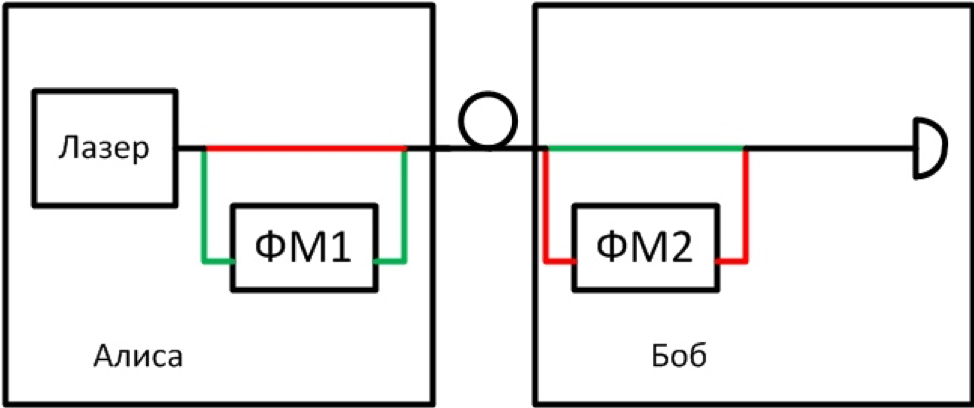
\includegraphics {Fig_2.png}
  \caption{Принципиальная схема системы квантовой коммуникации с фазовым кодированием [13]}
  \label{fig:Fig_2}
\end{figure}

Испущенный лазером импульс разделяется Алисой на две одинаковых части при помощи светоделителя: одна идет по "короткому" пути (красный1) и проходит через первый фазовый модулятор (ФМ1), а второй по "длинному" пути (зеленый1). Информация кодируется изменением фазы в ФM1. После прохождения по линиям связи, импульсы приходят в такой же интерферометр на стороне Боба, где снова разделяются на две части, формируя три вида импульсов. Первый, прошедший дважды по "короткому" пути (зеленый 2) и последний, дважды прошедший по "длинному" (красный 2), не несут никакой информации. Средний является результатом интерференции импульсов, прошедших пути красный1-красный2 и зеленый1-зеленый2. Чтобы детектировать полученный в результате интерференции импульс необходимо его отделить от мощного импульса красный1-зеленый2 с помощью электро-оптического затвора ЭЗ и направить на детектор одиночных фотонов ДОФ. Импульс красный1-зеленый2 впоследствии может использоваться в качестве опорного импульса, то есть сигнализировать о факте прибытия квантового импульса.

%%%%%%%%%%%%%%%%%%%%%%%%%%%%%%%%%%%%%%%%%%%%%%%%%%%%%%%%%%%%%%%%%%%%%%%%%%%%%%%%%%%%%%%%%%%%%%%%%%%%%%%%%%%%%%%%%

\section{Системы квантовой коммуникации на боковых частотах модулированного излучения} \label{sec:ch1/sec4}

Метод квантового распределения ключа на боковых частотах модулированного излучения (КРКБЧ) был впервые предложен в работе [16] и развивался в работах [17, 18]. Основными особенностями являются: простота по сравнению с указанными выше аналогами благодаря исключению влияния поляризации, а также отказу от работы по принципу интерферометра Маха-Цендера ввиду необходимости постоянного проведения достаточно сложной юстировки; высокая скорость передачи информации; возможность спектрального уплотнения сигналов с квантовыми состояниями.

 
Генерация криптографического ключа по протоколу B92 в данной системе происходит следующим образом [19]:


Когерентное монохроматическое излучение генерируется лазерным источником (Лазер) на длине волны порядка 1550 нм (в третьем окне прозрачности кварца-диапазоне длин волн с наименьшими вносимыми средой потерями). Излучение подвергается фазовой модуляции с помощью модулятора Алисы (ФМ1). В простейшем случае применяется периодическая синусоидальная фазовая модуляция. В результате модуляции в спектре сигнала появляются две боковые частоты, отстоящие от основной частоты оптического сигнала на величину частоты модулирующего радиочастотного сигнала. Далее световой пучок ослабляется с помощью аттенюатора до уровня энергии одиночных фотонов. Для передачи квантового сигнала используются боковые частоты при выполнении условия $\mu \ll 1$ ( $\mu$ - среднее число фотонов в импульсе). Мощность излучения на боковых частотах должна быть значительно ниже, чем на центральной частоте. Ослабленный сигнал на центральной частоте представляет собой опорный световой пучок. Кодирование происходит благодаря внесению в модулирующий сигнал некоторого фазового сдвига. Блок отправителя соединен с блоком получателя волоконно-оптической линией связи телекоммуникационного стандарта (SMF-28 или аналогичный). При достижении приёмного модуля сигнал подвергается повторной фазовой модуляции (ФМ2) по аналогии с модулем отправителя. При этом в модулирующий сигнал также вносится случайный фазовый сдвиг, не зависящий от сдвига, использованного на стороне отправителя. Мощность излучения на боковых частотах зависит от значений фазового сдвига, внесенных на передающем устройстве и приемном устройстве. Если они совпали, т.\:е. разность фаз двух модулирующих радиочастотных сигналов равна нулю ($\phi$A-$\phi$В=$0$), на боковых частотах наблюдается конструктивная интерференция, и мощность оптического сигнала отлична увеличивается. В случае, когда модулирующие радиочастотные сигналы Алисы и Боба находятся в противофазе, т.\:е. разность фаз модулирующих сигналов равна $\pi$ ($\phi$A-$\phi$В=$\pi$), наблюдается деструктивная интерференция, и мощность сигнала на боковых частотах уменьшается до нуля [16]. На основании срабатываний детектора одиночных фотонов (ДОФ) формируется <<сырой>> ключ.
 
 
При конструктивной интерференции значениям выбранных сдвигов фаз (0 или π) соответствуют, по договоренности, биты (0 или 1). Боб по открытому каналу сообщает Алисе моменты времени, когда совпали их сдвиги фаз, и та, в свою очередь, отбрасывает лишнюю информацию. Так генерируется <<просеянный>> ключ, который подлежит процедуре коррекции ошибок. 

 \begin{figure}[ht]
  \centering
  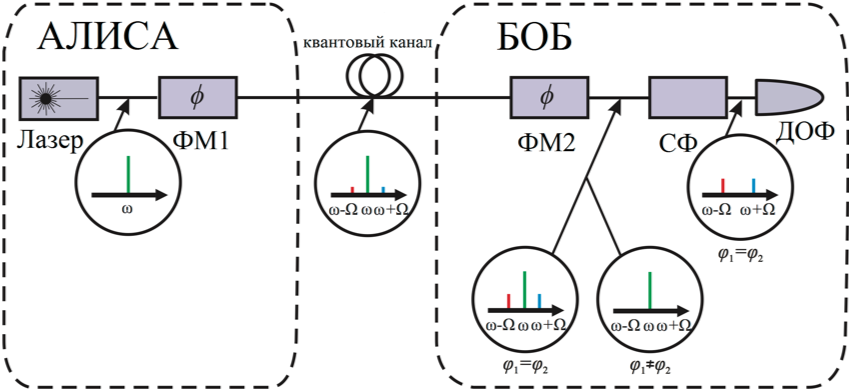
\includegraphics {Fig_3.png}
  \caption{Принципиальная схема системы квантовой коммуникации на боковых частотах модулированного излучения}
  \label{fig:Fig_3}
\end{figure}


%%%%%%%%%%%%%%%%%%%%%%%%%%%%%%%%%%%%%%%%%%%%%%%%%%%%%%%%%%%%%%%%%%%%%%%%%%%%%%%%%%%%%%%%%%%%%%%%%%%%%%%%%%%%%%%%%%

\section{Измерительное оборудование в системах квантовой коммуникации} \label{sec:ch1/sec5}


Системы квантовой коммуникации (СКК) оперируют с крайне низкоинтенсивным излучением в волоконно-оптических линиях связи (ВОЛС), где в среднем в каждом тактовом отсчете сосредоточена энергия не более одного фотона. Детекторы одиночных фотонов (ДОФ) способны улавливать подобные сигналы, что делает их неотъемлемой частью СКК. Условно ДОФ можно разделить на две группы: широкодоступные и узкоспециализированные. Очевидно, что детекторы из второй группы, например, криогенные термоэлектрические детекторы (QVD) [17] и детекторы, основанные на поглощении в холодном атомном паре [18], не могут быть использованы серийно в производстве систем СКК. Поэтому в данном разделе рассматриваются основные виды которые широко применимых ДОФ:

\begin{enumerate}
	\item использующие нанопроволоку в режиме сверхпроводимости (superconducting nanowire single-photon detector, SNSPD);
	\item использующие полевой транзистор, обогащенный квантовыми точками, с оптическим затвором (quantum-dot optically gated field-effect transistor, QDOGFET);
	\item на основе регистрации лавинных срабатываний в лавинных фотодиодах при попадании однофотонного излучения (single-photon avalanche diode, SPAD);уаау]
	\item использующий джозефсоновский переход (superconducting-tunnel-junction detector, STJ);
	\item использующие сенсор, реагирующий на переход материала из сверхпроводящего состояния в проводящее (transition-edge sensor, TES);
	\item счетчик фотонов видимого света (visible-light photon counter, VLPC) и твердотельный фотоумножитель (solid-state photomultiplier, SSPM).
\end{enumerate}

На основании сравнительной характеристики будет оценена целесообразность использования данных ДОФ для СКК.

\subsection{Лавинные фотодиоды для однофотонного излучения} \label{subsec:ch1/sec5/sub1}

ДОФ этого типа используют процесс, схожий с тем, что происходит в фотоумножителе [19]. В отличие от фотоумножителя, в фотодиоде поглощение фотона рождает электрон-дырочную пару, которая порождает аналогичное увеличение числа заряженных частиц благодаря напряжению, приложенному вдоль кристаллической решетки полупроводника. Лавинные фотодиоды, используемые для ИК излучения, имеют низкие типичные показатели квантовой эффективности 10-20~\%  (доля излучения, которая успешно переведена в электрический сигнал и зарегистрирована). Они также характеризуются достаточно высокими значениями частоты темновых срабатываний (ложные срабатывания детектора в отсутствие входящего излучения, зачастую вызванного теплом окружающей среды), поэтому диод охлаждают до 210-250 К, например, термоэлектрическими охладителями. Даже в этом случае уровень темновых отсчётов для коммерческих ДОФ данного типа составляет порядка 1-10 кГц. Для лавинных детекторов характерна остаточная пульсация, когда электроны из лавины ненадолго <<застревают>>, например, в дефектах и, освобождаясь, порождают вторичные лавины. Необходимо некоторое время для выхода в штатный режим работы, поэтому у таких диодов обычно относительно высокое мертвое время (время, когда детектор сразу после срабатывания не может повторно зарегистрировать сигнал), что может ограничить тактовую частоту следования квантовых сигналов в СКК.

\subsection{ДОФ, использующий полевой транзистор, обогащенный квантовыми точками, с оптическим затвором} \label{subsec:ch1/sec5/sub2}

Совмещение полевого транзистора с оптическим затвором из квантовых точек, расположенных между стоком и истоком, позволяют добиться регистрации одиночных ИК фотонов [20]. Квантовые точки захватывают заряженные частицы, рожденные падающим светом, изменяя приложенное электрическое поле, что ведет к изменению протекающего по транзистору тока - по данному изменение и производится детектирование сигнала. Однако низкое быстродействие данного детектора не соответствует типовым системам СКК. Квантовая эффективность не превышает 15~\%, а максимальная тактовая частота следования квантовых сигналов составляет всего 50 кГц. Кроме того, для работы данного ДОФ необходимы низкие рабочие температуры (от 70 К и ниже). При этом вероятность темновых срабатываний относительно высока.

\subsection{ДОФ, использующие сверхпроводящую нанопроволоку} \label{subsec:ch1/sec5/sub3}

Данный тип ДОФ является одним из самых быстрых. Он способен регистрировать квантовые состояния с частотой следования до единиц гигагерц [21]. Основным элементом здесь служит площадка со сверхпроводящей тонкой проволокой (superconducting nanowire), запитанная током немного меньшим, чем критический, выше которого волокно выходит из сверхпроводящего режима. В таком случае поглощенный фотон оставляет небольшой участок нагретым и, соответственно, в проводящем состоянии. Поэтому ток начинает огибать этот участок с нормальной проводимостью. В результате ток превышает критическое значение, что приводит к переходу в проводящий режим всего участка вдоль ширины волокна. Появление участка с сопротивлением выражается в соответствующем скачке напряжения во внешней цепи, что и свидетельствует о детектировании фотона. Поскольку данный механизм детектирования требует очень узкой проволоки (порядка 100 нм), его складывают меандром, для создания эффективной рабочей поверхности. Для повешения эффективности детектирования, сверху волокно покрывают отражающей поверхностью, что в итоге образует резонатор, значительно улучшающий характеристики детектора. В подобных устройствах используют в основном проволоку из нитрида ниобия, однако из-за высокого коэффициента отражения у данного материала - необходимо просветляющее покрытие, благодаря которому можно добиться высокого значения квантовой эффективности до 60~\%. Ввиду того, что детектор работает в сверхпроводящем режиме, ему необходимы низкие рабочие температуры менее 4 К. В этом режиме он характеризуется низким уровнем темновых отсчётов ($10^{-2}$-$10^2$ Гц), что важно при реализации дальнодействующих СКК.

\subsection{ДОФ, использующие джозефсоновский переход} \label{subsec:ch1/sec5/sub4}

Основным элементов для данного типа детекторов служит джозефсоновский переход - две части сверхпроводника разделенных сверхтонким (порядка 1 нм) диэлектриком, см., например, [22]. Фотон, падающий на сверхпроводящую область, вызывает распад большого числа куперовских пар электронов (квазичастицы), т.\:к. его энергия в тысячи раз больше энергии связи. Свободные электроны после распада пар способны туннелировать через диэлектрик во вторую часть сверхпроводника с крайне высокой вероятностью. Поскольку рабочая температура детектора на порядок ниже переходной температуры в сверхпроводящее состояние, куперовских пар распавшихся за счет иных процессов, нежели за счет поглощенных сигнальных фотонов, значительно меньше, что позволяет однозначно зарегистрировать однофотонное излучение. Таким образом, данный вид детекторов позволяет детектировать фотоны с эффективностью, не превышающей 45~\%, частотой следования фотонов порядка десятков кГц, однако при крайне низких рабочих температурах 0,37 К.

\subsection{Детекторы одиночных фотонов, использующий сенсор, реагирующий на переход материала из сверхпроводящего состояния в проводящее} \label{subsec:ch1/sec5/sub5}

Данный сенсор работает по принципу болометра: при поглощении излучения повышается температура сенсора [23]. Для достижения чувствительности к одиночным фотонам необходима крайне малая теплоемкость поглощающего материала, и температурный сенсор должен обладать чрезвычайно высоким откликом на малое изменение температуры. Это возможно при изготовлении сенсора из тонкого сверхпроводящего материала, и его работы точно при температуре перехода из сверхпроводящего режима в обычный (порядка 100 мК) так, что небольшое изменение температуры отражается в значительном изменении сопротивления. Большей точности измерения колебаний сопротивления можно добиться, используя сверхчувствительный магнитометр, основанный на сверхпроводящем квантовом интерферометре (SQUID). Данный вид детекторов обладает самым большим показателем квантовой эффективности среди прочих - 95~\% для фотонов в ИК области. Несмотря на это, максимальная частота следования фотонов ограничена порогом в 100 кГц.

\subsection{ДОФ видимого света и твердотельный фотоумножитель} \label{subsec:ch1/sec5/sub6}

С точки зрения квантовой эффективности, данный детектор может сравниться с предыдущим, но в области видимого света, где она достигает 90~\% [24]. Принцип работы схож с лавинным диодом, но в данном случае не электрон, а дырка, выбитая падающим излучением, ускоряется к легированной части полупроводника, где уже рождает электронную лавину. Несмотря на высокое значение квантовой эффективности, остальные параметры достаточно низки: максимальная скорость детектирования фотонов составляет 100 кГц, частота темновых срабатываний велика - не менее 20 кГц. Схожими по конструкции и принципу работы являются твердотельные фотоумножители [25]. Они обладают широкой спектральной восприимчивостью, что, в свою очередь, требует экранирования от дальнего ИК излучения, которое не представляет интереса.

\subsection{Cравнительная характеристика ДОФ для СКК} \label{subsec:ch1/sec5/sub7}

Ниже представлена таблица 1, в которой представлены ключевые параметры детекторов, описанных в предыдущих разделах.

\begin{table} [htbp]
	\centering
	\caption{Сравнительные характеристики распространённых ДОФ.}
	\label{tab:SPD_compare}
	\begin{tabular}{| c | c | c | c | c |}
	
	 \hline \makecell{Тип \\детектора} & \makecell{Рабочая T,\\~K} & \makecell{Квантовая \\эффективность,\\~\%} & \makecell{Максимальная \\частота \\регистрации \\квантовых \\сигналов} & \makecell{Темновые отсчеты, \% \\(от частоты \\регистрации \\квантовых \\сигналов)}   \\ \hline
	  SPAD         & 210-250    & < 20    & 300 МГц     & < 0,1   \\ \hline
	  STJ	   	   & < 1        & > 45    & 10 кГц  	& < 0,1      \\ \hline
	  QDOGFET      & < 80       & < 15    & 50 кГц      & < 1       \\ \hline
	  TES          & < 0,1      & > 90    & 1 МГц       & < 0,01       \\ \hline
	  \makecell{VLPC\\/SSPM} & < 10      & < 90    & 100 кГц       & < ~20      \\ \hline
	  SNSPD          & < 10      & < 60    & 3 ГГц       & < 0,0001       \\ \hline
	  
	\end{tabular}
\end{table}

На основе выполненного сравнения можно сделать следующие выводы. 


Лавинные фотодиоды для однофотонного излучения (SPAD) рекомендуется использовать для СКК. Это объясняется тем, что они работают при температурах, которые возможно обеспечить без дополнительного охлаждающего криогенного оборудования, имеют оптоволоконный интерфейс и обладают максимальной частота регистрации квантовых сигналов ниже, чем предполагаемая частота смены фазы квантовых состояний электроникой СКК. Относительно низкая квантовая эффективность и высокий уровень темновых срабатываний, однако, позволяет использовать данный вид детекторов на малых и средних дистанциях при небольших потерях в линиях ВОЛС (до 10-15 дБ).


ДОФ, использующий джозефсоновский переход (STJ) не рекомендуется использовать для приложений СКК ввиду низкой максимальной частоты регистрации квантовых сигналов и крайне низких рабочих температур, обеспечение которых является сложным технологическим процессом, увеличивающим их стоимость.


ДОФ, использующий полевой транзистор, обогащенный квантовыми точками, с оптическим затвором (QDOGFET) не рекомендуется использовать для приложений СКК по причине низкой скорости срабатывания.


ДОФ, использующий сенсор, реагирующий на переход материала из сверхпроводящего состояния в проводящее (TES) не рекомендуется использовать для приложений СКК ввиду низкой максимальной частоты регистрации квантовых сигналов и крайне низких рабочих температур, обеспечение которых является сложным технологическим процессом.


Счетчик фотонов видимого света (VLPC) и твердотельный фотоумножитель (SSPM) не рекомендуется использовать для приложений СКК по причине низкой скорости срабатывания.


ДОФ, использующий сверхпроводящую нанопроволоку (SNSPD) рекомендуется использовать для приложений СКК, т.\:к. они работают при температурах жидкого гелия, что возможно обеспечить в свою очередь и компенсируется высокими ключевыми показателями, которые обеспечат штатную работу системы СКК. Данный тип детекторов следует использовать в каналах с относительно высокими потерями (от 15 дБ). 

%%%%%%%%%%%%%%%%%%%%%%%%%%%%%%%%%%%%%%%%%%%%%%%%%%%%%%%%%%%%%%%%%%%%%%%%%%%%%%%%%%%%%%%%%%%%%%%%%%%%%%%%%%%%%%%%%

\section{Атаки злоумышленника} \label{sec:ch1/sec6} 

В действительности существует значительное отличие между моделями, которые используются для теоретического подтверждения возможности формирования абсолютно стойких ключей квантовыми методами, и практическими реализациями таких систем. Во втором случае всегда существует малая вероятность того, что система или устройства будут иметь отклонение от усредненных параметров. Другим важным фактором является то, что компоненты таких систем зачастую не разрабатывались специально под данную задачу и поэтому потенциально могут иметь ряд других режимов, характеристик и свойств в других условиях и для применения в изначальных целях. Этими нюансами может воспользоваться злоумышленник, который хочет вопреки ограничениям остаться незамеченным и при этом получить максимальное количество ключевой информации. Известны ряд неидеальностей, которые, если их не учитывать, позволяют злоумышленнику добиваться значительных результатов. Такой подход и используемые для этого методы называются \textit{квантовым взломом} (quantum hacking). Это могут быть атаки злоумышленника с разделением пучка фотонов, формируемого в результате ослабления когерентного лазерного излучения, в котором статистика числа фотонов в импульсе подчиняется распределению Пуассона. Это значит, что существует ненулевая вероятность обнаружить в одном импульсе многофотонные состояния, отделить часть энергии и зафиксировать квантовое состояние, оставшись незамеченным. Другим потенциально уязвимым звеном систем квантовой коммуникации является детектор одиночных фотонов. Ниже обосновывается уязвимость систем при использовании таких устройств и возможные типы атак злоумышленника с использованием данной уязвимости. 

%	\subsection{Атака с разделением пучка фотонов}  \label{subsec:ch1/sec6/sub1}


%	\subsection{Атака типа перехват} \label{subsec:ch1/sec6/sub2}


%	\subsection{Атака типа перехват-пересылка} \label{subsec:ch1/sec6/sub3}


\subsection{Атака на детектор на основе ЛФД} \label{subsec:ch1/sec6/sub4}

Первым этапом проведения атаки с навязыванием ключа является определение возможности выведения детектора из режима счета фотонов (режима Гейгера). Известно, что вольт-амперная характеристика лавинного фотодиода имеет вид, представленный на рисунке \ref{fig:APDs_VA}.    

 \begin{figure}[ht]
  \centering
  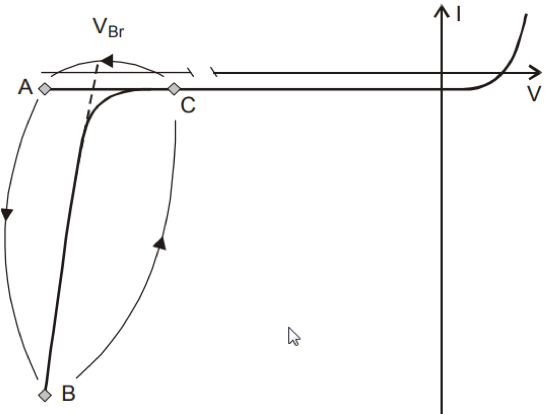
\includegraphics{APDs_VA.png}
  \caption{Вольт-амперная характеристика ЛФД}
  \label{fig:APDs_VA}
\end{figure}


Лавинный фотодиод работает при обратном напряжении смещения $-V_{bias}$ близком к напряжению пробоя $-V_{breakdown}$. Типичная величина находится в диапазоне от -40~В до -60~В. При величине обратного напряжения смещения ниже напряжения пробоя ЛФД находится в линейном режиме, где величина фототок $I_{APD}$ линейно зависит от падающей оптической мощности. При увеличении величины обратного смещения выше напряжения пробоя ЛФД переходит в режим счета фотонов, или режим Гейгера. В этом режиме даже энергии единиц фотонов достаточно для формирования лавины зарядов и резкого скачка фототока. При превышении некоторого порогового значения $I_{det}$, регулируемого уровнем срабатывания компаратора, формируется электрический импульс, который и интерпретируется, как регистрация одиночного фотона. 

 \begin{figure}[ht]
  \centering
  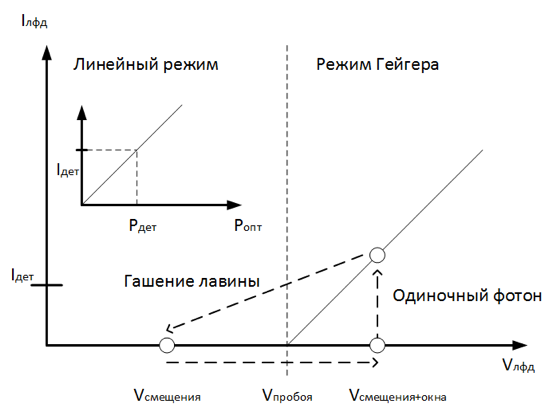
\includegraphics{Vbreakdown}
  \caption{Граница между режимами работы ЛФД при подаче обратного напряжения смещения}
  \label{fig:Vbreakdown}
\end{figure}

Гашение лавины в самом простом случае происходит благодаря последовательно подключенному в цепь резистору, как показано на рисунке \ref{fig:Quenching}. Существуют также схемы активного гашения лавины.  

 \begin{figure}[ht]
  \centering
  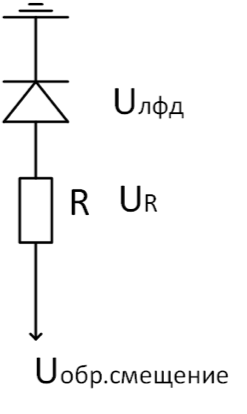
\includegraphics{Quenching}
  \caption{Принципиальная электрическая схема подключения ЛФД для регистрации одиночных фотонов}
  \label{fig:Quenching}
\end{figure}


Для снижения уровня шумов срабатываний ДОФ на базе ЛФД функционируют в режиме стробирования, когда в момент ожидаемого прибытия фотона на диод подается дополнительное напряжение в форме импульса, т.\:н. окно срабатывания $-V_{gate}$, величиной около 3~В. Благодаря этому импульсу диод переходит из линейного режима при величине напряжении $-V_{bias}$, в котором он прибывает относительно длительное время порядка единиц микросекунд, в режим счета фотонов, где $-V_{bias+gate} < - V_{breakdown}$.  

\subsection{Атака с навязыванием ключа ( Faked-state attack)} \label{subsec:ch1/sec6/sub5}


В работе показана полноценная реализация атаки с использованием уязвимости детектора на основа ЛФД. Злоумышленник имеет модифицированный приёмный узел, аналогичный блоку получателя м связанный с модифицированным узлом отправителя. Первый принимает квантовые состояния от легитимного отправителя и те случаи, где происходит совпадения посылает в модифицированный узел отправителя. Там используется интенсивное оптическое излучение для контроля детектора фотонов и формирования срабатываний в требуемых злоумышленнику отсчетах. Таким образом, он является незамеченным обладателем ключевой информации. 

 \begin{figure}[ht]
  \centering
  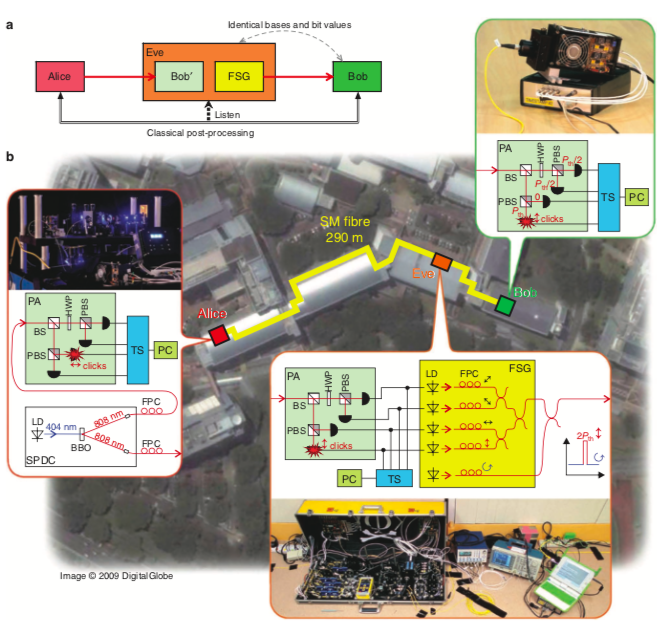
\includegraphics[scale=0.5]{FSA.png}
  \caption{Принципиальная схема проведения атаки с поддельными состояниями}
  \label{fig:FSA}
\end{figure}

\pagebreak
%%%%%%%%%%%%%%%%%%%%%%%%%%%%%%%%%%%%%%%%%%%%%%%%%%%%%%%%%%%%%%%%%%%%%%%%%%%%%%%%%
%	\subsection{Атака на SNSPD} \label{subsec:ch1/sec6/sub6}


%%%%%%%%%%%%%%%%%%%%%%%%%%%%%%%%%%%%%%%%%%%%%%%%%%%%%%%%%%%%%%%%%%%%%%%%%%%%%%%%%%%%%%%%%%%%%%%%%%%%%%%%%%%%%%%%%%

\section{Известные контрмеры против атак на измерительное оборудование} \label{sec:ch1/sec7}

Существует ряд решений для предотвращения атаки с навязыванием ключа. Ниже перечислены основные. Однако, следует отметить, что строгое доказательство секретности, а также многочисленные экспериментальные работы, подтверждающие практическую ценность есть только у предпоследнего подхода. Остальные контрмеры требуют исследования в стенах лабораторий, практикующих квантовый взлом. 

\subsection{Статистика счета фотонов} \label{subsec:ch1/sec7/sub1}

В работе предложена контрмера, основанная на наборе статистики фотонов, которые поступают на светоделитель с двумя детекторами. В случае применения атаки с <<ослеплением>> изменяется количество одновременных совпадений на этих двух детекторах относительно их нормального режима работы. 

 \begin{figure}[ht]
  \centering
  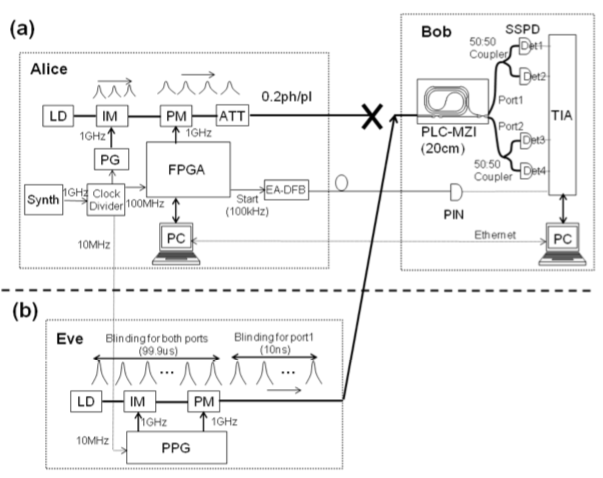
\includegraphics[scale=0.5]{PhotonStatistics.png}
  \caption{Принципиальная схема контрмер на основе статистики фотонов}
  \label{fig:PhotonStatistics}
\end{figure}

\subsection{Измерение фототока} \label{subsec:ch1/sec7/sub2}

Очевидным решением является активный мониторинг фототока, протекающего в ЛФД при попадании на него оптического излучения, и наблюдении лавинного пробоя, как показано на рисунке \ref{fig:Photocurrent}. 

 \begin{figure}[ht]
  \centering
  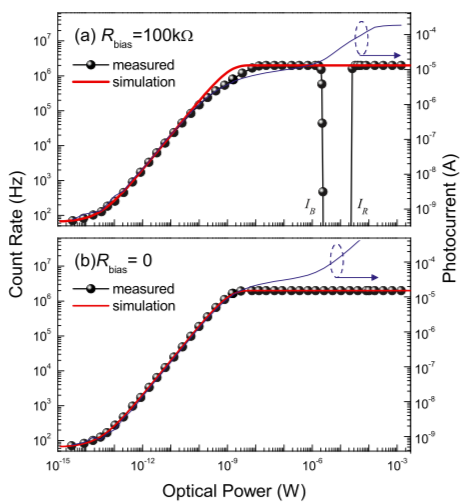
\includegraphics[scale=0.5]{Photocurrent.png}
  \caption{Зависимость количество отсчетов и фототока от интенсивности падающего излучения}
  \label{fig:Photocurrent}
\end{figure}
\pagebreak

\subsection{MDI-протокол} \label{subsec:ch1/sec7/sub3}

В работе предложен метод, в основе которого лежит предположение о том, что измерительный узел доступен злоумышленнику, который при этом знает какие из детекторов произвели срабатывание и в какой временной отсчет, однако при этом не имеют информации о том, какое квантовое состояние в блоках Алисы и Боба применялось. Это достигается за счет интерференции слабых когерентных импульсов на светоделителе внутри недоверенного узла регистрации. В процессе постселекции легитимные пользователи выявляют результат однофотонной интерференции, который привел к срабатыванию, и соотвествующие ему состояние, которые были использованы. Такой подход получил название MDI (measuerement-device-independent) и нашел широкое применение для исследований, благодаря устойчивости к атакам на измерительное оборудование. Однако, на практике ввиду чрезвычайному усложнению оптической схемы и условий, при которых наблюдается интерференция, почти не применяется в условиях близких к реальным. 


 \begin{figure}[ht]
  \centering
  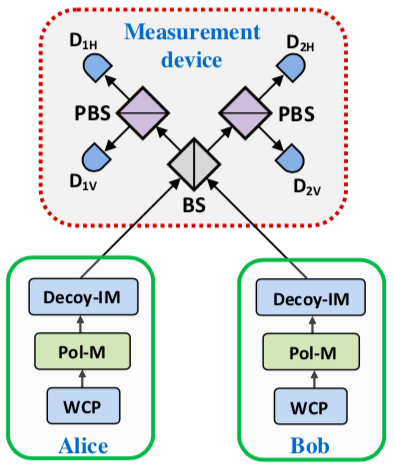
\includegraphics[scale=0.5]{MDI_scheme.png}
  \caption{Принципиальная схема системы с независимым измерительным устройством MDI}
  \label{fig:MDI_scheme}
\end{figure}


\subsection{Twin-Field протокол} \label{subsec:ch1/sec7/sub4}


Развитием темы MDI с применением фазовых состояний является протокол Twin-Field (близнецовые поля), где так же применяется анонсирование измерительным узлом, доступным злоумышленнику, результата интерференции когерентных состояний на светоделителе, которые приводят к срабатыванию детекторов одиночных фотонов. Отличительной особенностью является то, что в отличие от MDI, где для минимизации корреляции по фазе последовательности импульсов от каждого из источников, используется их рандомизация, то есть изменение фазы случайным образом, в протоколе Twin-Field используется результат интерференции когерентных состояний с определением секторов на фазовой плоскости и отбрасыванием фазовых состояний, соответствующих разным секторам в процессе постоработки.

 
 \begin{figure}[ht]
  \centering
  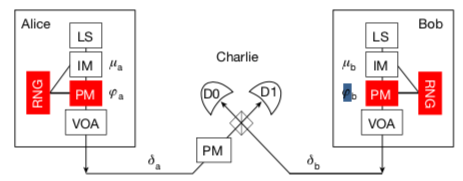
\includegraphics[scale=0.5]{TF_scheme.png}
  \caption{Принципиальная схема системы с независимым измерительным устройством}
  \label{fig:TF_scheme}
\end{figure}
%%%%%%%%%%%%%%%%%%%%%%%%%%%%%%%%%%%%%%%%%%%%%%%%%%%%%%%%%%%%%%%%%%%%%%%%%%%%%%%%%%%%%%%%%%%%%%%%%%%%%%%%%%%%%%%%%%

\section{Выбор направления исследований. Цели и задачи работы} \label{sec:ch1/sec8}

Системы квантовой коммуникации на боковых частотах модулированного излучения зарекомендовали себя, как перспективное направление коммерчески доступных устройств квантового распределения ключа с практически значимыми характеристиками мирового уровня, подтвержденными в ряде научных публикаций в международных изданиях, формализованным доказательством безусловной секретности используемого протокола, применением на нескольких полигонах, развернутых на территории Российской Федерации, совместной с ведущими компаниями в области телекоммуникационной связи, банковского сектора и региональными инжиниринговыми центрами. 


С научной и инженерной точки зрения данный класс систем имеет большой задел:

\begin{enumerate}
	\item Экспериментальная демонстрация передачи квантовых состояний на основе технологии квантовой коммуникации на боковых частотах модулированного излучения в телекоммуникационной линии связи дальностью свыше 250 км. 
	\item Разработка функциональной схемы и экспериментальная реализация оптико-электронного устройства квантовой передачи информации на боковых частотах, включающую подсистему непрерывной синхронизации модулей отправителя и получателя, подсистему компенсации неконтролируемого изменения поляризации в оптическом волокне.
	\item Экспериментально продемонстрировано спектральное уплотнение каналов на боковых частотах. 
	\item Разработка функциональной схемы и экспериментальная реализация оптико-электронного устройства квантовой передачи информации на боковых частотах, включающую подсистему непрерывной синхронизации модулей отправителя и получателя, подсистему компенсации неконтролируемого изменения поляризации в оптическом волокне.
	\item Экспериментальная демонстрация применимости данной технологии для квантового распределения ключа в открытом пространстве, а не только в волоконно-оптических линиях связи. 
\end{enumerate}


Однако, устойчивость квантовых систем передачи информации на боковых частотах к воздействию нелегитимного пользователя на измерительной оборудование ранее не была исследована. 


{\aim} данной работы является исследование возможностей злоумышленника по получению секретного ключа с использованием атак на измерительное оборудование систем квантовой коммуникации на боковых частотах и разработка методов противодействия атакам.


Для~достижения поставленной цели ставились следующие {\tasks}:
\begin{enumerate}
  \item Исследование устойчивости детектора одиночных фотонов, применяемого в системах квантовой коммуникации на боковых частотах, к атакам с выведением из режима Гейгера (<<ослеплением>>). 

  \item Оценка возможностей злоумышленника при атаке с выведением из режима Гейгера для систем квантовой коммуникации на боковых частотах. 

  \item Разработка оптической схемы системы квантовой коммуникации, устойчивой к атакам на измерительное оборудование. 

  \item Разработка протокола квантовой рассылки ключа, устойчивого к атаке на измерительное оборудование. 

\end{enumerate}
           % Глава 1
\chapter{Исследование устойчивости системы квантовой коммуникации на боковых частотах к атакам на измерительное оборудование}  \label{ch:ch2}


\section{Детектор в составе системы} \label{sec:ch2/sec1}

В зависимости от поставленных целей и решаемых задач в состав систем квантовой коммуникации включают в основном два типа детекторов одиночных фотонов, сравнительная характеристика которых дана в главе \ref{sec:ch1/sec5}. Для магистральных дистанций от 100~км, либо для обеспечения высокой скорости формирования квантовых кодирующих последовательностей применяют сверхпроводниковые ДОФ (SNSPD). Для внутригородских дистанций до 100~км с потерями в линиях связи менее 15~дБ обычно применяют более компактный, простой в использовании ДОФ на базе лавинного фотодиода (SPAD), однако его типовые характеристики на порядок уступают характеристикам сверхпроводникового ДОФ. 


В СКК на боковых частотах применяется коммерчески доступный детектор модели ID210, разработанный компанией idQuantique. Его отличительными особенностями являются:
\begin{enumerate}
	\item Поддержка высокой частоты стробирующих импульсов - до 100~МГц
	\item Возможность подачи стробирующих импульсов от внешнего устройства (External gating mode)
	\item Широкий диапазон настройки ширины окна срабатывания (gate) - от 0,5~нс до 25~нс
	\item Выставление задержки открытия окна срабатывания относительно стробирующего импульса (Trigger delay) в диапазоне до 10~нс с высоким разрешением во времени - 10~пс 
	\item Возможность выставления <<мертвого времени>> в широком диапазоне - от 0,1~мкс до 100~мкс
	\item Возможность регулировки квантовой эффективности с шагом 2,5~\% в диапазоне от 5~\% до 25~\%
	\item Полупроводниковая структура ЛФД - InGaAs/InP
	\item Относительно низкий уровень темнового счета при заданных параметрах квантовой эффективности
\end{enumerate}


В ходе исследования для обеспечения реалистичных условий атаки злоумышленника на измерительное оборудование в составе СКК устройство рассматривалось, как <<черный ящик>>, то есть оно не вскрывалось и не производились манипуляции с внутренними платами и микросхемами. Все настройки детектора выставлялись в соответствии со штатным режимом для систем квантовой коммуникации на боковых частотах модулированного излучения. Основные настройки вынесены в таблицу \ref{tab:ID210_setups}.  




\begin{table} 
	\centering
	\caption{Типовые настройки детектора ID210 в составе СКК}
	\label{tab:ID210_setups}
		\begin{tabular}{|c|c|c|}
			\hline
				№  				& Параметр    				 & Значение     \\
			\hline
				1 				& Квантовая эффективность,~\% 	 & 10 		 \\
			\hline 

				2 				& Частота стробирования,~Гц 		 & $10^8$   \\
			\hline

				3 				& Ширина окна,~нс & 5 	     \\
			\hline

				4 				& <<Мертвое>> время,~нс  & 100 		  \\
			\hline

				5 				& Частота темновых срабатываний,~Гц & 200 		  \\

			\hline
		\end{tabular}
\end{table}




%%%%%%%%%%%%%%%%%%%%%%%%%%%%%%%%%%%%%%%%%%%%%%%%%%%%%%%%%%%%%%%%%%%%%%%%%%%%%%%%%%%%%%%%%%%%%%%%%%%%%%%%%%%%%%%%%

\section{Выведение детектора из режима Гейгера} \label{sec:ch2/sec2}

Первым этапом проведения атаки с навязыванием ключа является определение возможности выведения детектора из режима счета фотонов (режима Гейгера). Известно, что вольт-амперная характеристика лавинного фотодиода имеет вид, представленный на рисунке \ref{fig:APDs_VA}.    

 \begin{figure}[ht]
  \centering
  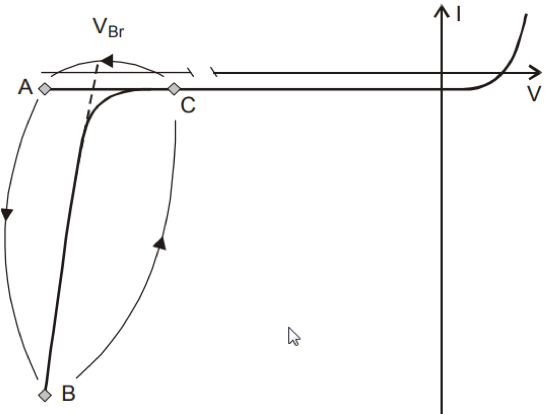
\includegraphics{APDs_VA.png}
  \caption{Вольт-амперная характеристика ЛФД}
  \label{fig:APDs_VA}
\end{figure}


Лавинный фотодиод работает при обратном напряжении смещения $-V_{bias}$ близком к напряжению пробоя $-V_{breakdown}$. Типичная величина находится в диапазоне от -40~В до -60~В. При величине обратного напряжения смещения ниже напряжения пробоя ЛФД находится в линейном режиме, где величина фототок $I_{APD}$ линейно зависит от падающей оптической мощности. При увеличении величины обратного смещения выше напряжения пробоя ЛФД переходит в режим счета фотонов, или режим Гейгера. В этом режиме даже энергии единиц фотонов достаточно для формирования лавины зарядов и резкого скачка фототока. При превышении некоторого порогового значения $I_{det}$, регулируемого уровнем срабатывания компаратора, формируется электрический импульс, который и интерпретируется, как регистрация одиночного фотона. 

 \begin{figure}[ht]
  \centering
  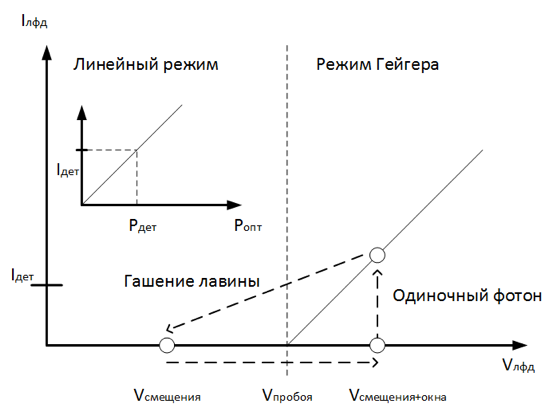
\includegraphics{Vbreakdown}
  \caption{Граница между режимами работы ЛФД при подаче обратного напряжения смещения}
  \label{fig:Vbreakdown}
\end{figure}

Гашение лавины в самом простом случае происходит благодаря последовательно подключенному в цепь резистору, как показано на рисунке \ref{fig:Quenching}. Существуют также схемы активного гашения лавины.  
 \begin{figure}[ht]
  \centering
  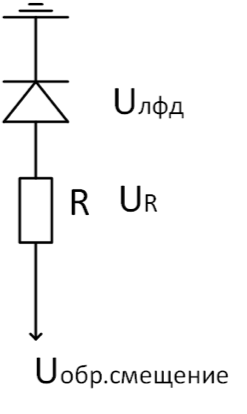
\includegraphics{Quenching}
  \caption{Принципиальная электрическая схема подключения ЛФД для регистрации одиночных фотонов}
  \label{fig:Quenching}
\end{figure}


Для снижения уровня шумов срабатываний ДОФ на базе ЛФД функционируют в режиме стробирования, когда в момент ожидаемого прибытия фотона на диод подается дополнительное напряжение в форме импульса, т.\:н. окно срабатывания $-V_{gate}$, величиной около 3~В. Благодаря этому импульсу диод переходит из линейного режима при величине напряжении $-V_{bias}$, в котором он прибывает относительно длительное время порядка единиц микросекунд, в режим счета фотонов, где $-V_{bias+gate} < - V_{breakdown}$.  

%%%%%%%%%%%%%%%%%%%%%%%%%%%%%%%%%%%%%%%%%%%%%%%%%%%%%%%%%%%%%%%%%%%%%%%%%%%%%%%%%%%%%%%%%%%%%%%%%%%%%%%%%%%%%%%%%

\section{Оптическая схема выведения детектора из режима Гейгера} \label{sec:ch2/sec3}

Для успешного осуществления атаки с навязыванием ключа злоумышленнику требуется манипулировать детектором, то есть форсировать срабатывания и их отсутствие в нужные моменты времени, при этом предполагается, что тип применяемого измерительного оборудования известен, но непосредственный доступ к нему отсутствует. В таких рамках модель атаки ограничивается возможностью воздействия на детектор только оптическими методами непосредственно из квантового канала. 


Известно, что в линейном режиме работы ЛФД при подачи на него постоянной оптической мощности увеличивается фототок, следовательно при подаче постоянного значения напряжение обратного смещения $-V_{bias}$ и при наличии в цепи гасящего лавину резистора, величина падения напряжения на резисторе растет, а на ЛФД снижается (рис.\ref{fig:Quenching}. Суть атаки с выведением детектора из режима Гейгера, или <<ослеплением>> ДОФ, сводится к тому, чтобы сместить режим работы относительно напряжения пробоя ЛФД. При таком подходе даже дополнительных импульсов $V_{gate}$ становится недостаточно и диод все время находится в режиме линейной зависимости фототока от величины мощности оптического излучения, падаюшего на него.  

Тем не менее, как указано на рисунке \ref{fig:Vbreakdown}, в линейном режиме остается возможность превысить пороговое значение фототока $I_{det}$ и сформировать импульс срабатывания детектора.

Таким образом, методика выведения детектора из режима счета фотонов в линейный режим для осуществления атаки с навязыванием ключа (\todo{<<Faked-state attack>>}) легко формализуется. Экспериментальное исследование уязвимости детектора одиночных фотонов к такому типа атак реализуется в три этапа, представленных на рисунке \ref{fig:Method_2.3}:

 \begin{enumerate}
	\item Определение величины постоянной оптической мощности, достаточной для выведения детектора из режима Гейгера
	\item Подстройка оптического импульса под окно срабатывания детектора одиночных фотонов
	\item Определение зависимости вероятности срабатывания детектора от величины энергии фотонов в импульсе
\end{enumerate}

 \begin{figure}[ht] 
  \centering
  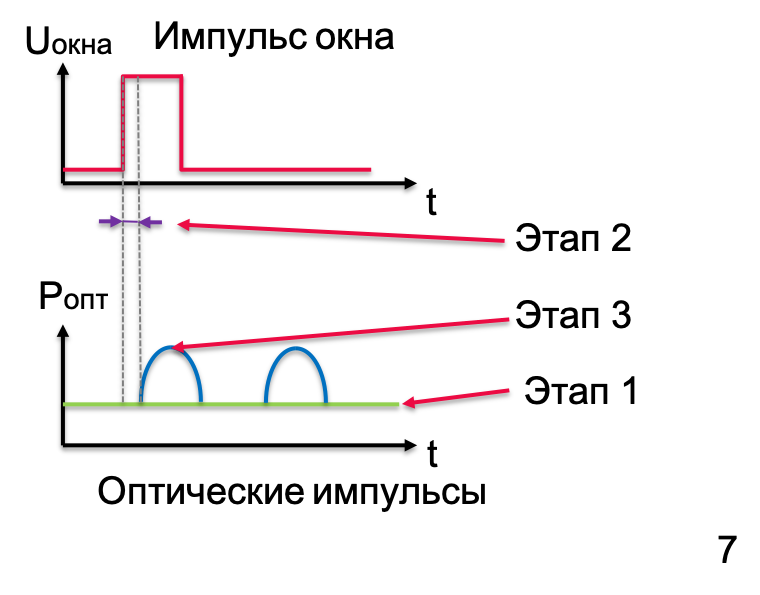
\includegraphics{Method_2.3.eps}
  \caption{Методика выведения детектора из режима Гейгера}
  \label{fig:Method_2.3}
\end{figure}

%
%  На рисунке \ref{fig:Scheme_2.3} представлена принципиальная оптическая схема для проведения исследования уязвимости детектора. 
%
% \begin{figure}[ht] 
%  \centering
%  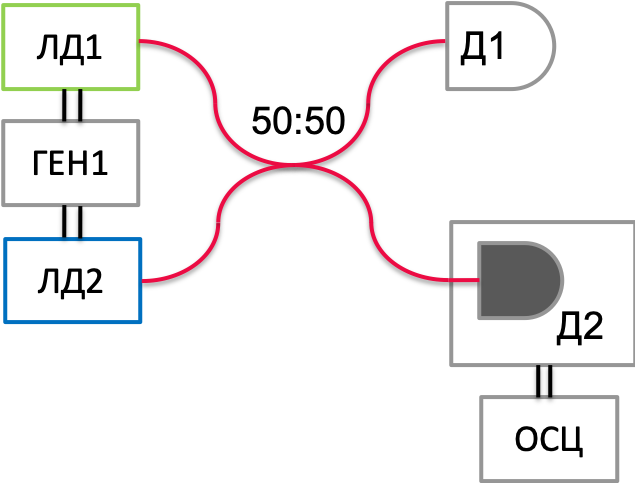
\includegraphics{Scheme_2.3.eps}
%  \caption{Принципиальная оптическая схема эксперимента}
%  \label{fig:Scheme_2.3}
% \end{figure}

%%%%%%%%%%%%%%%%%%%%%%%%%%%%%%%%%%%%%%%%%%%%%%%%%%%%%%%%%%%%%%%%%%%%%%%%%%%%%%%%%%%%%%%%%%%%%%%%%%%%%%%%%%%%%%%%%

\section{Корреляция оптической мощности в плечах светоделителя} \label{sec:ch2/sec4}


Для того, чтобы одновременно производить воздействие оптическим излучением на исследуемый детектор одиночных фотонов и фиксировать величину этого воздействия в оптической схеме используется светоделитель 2х2 с коэффициентом деления 50:50. Один выход подключен к детектору Д2, второй к измерителю оптической мощности Д1, как показано на рисунке \ref{fig:Scheme_2.4}. Однако, обычно в волоконно-оптических элементах наблюдается небольшое отклонение основных величин, характеризующих устройство, от паспортных значений. Для того, чтобы скорректировать это отклонение, при помощи двух измерителей оптической мощности фиксируется величина оптической мощности на обоих выходах светоделителя и находится разница между двумя величинами в зависимости от напряжения, подаваемого с генератора ГЕН1 (Agilent 81110A) на лазерный диод ЛД1, применяемый для выведения детектора и режима Гейгера.   

 \begin{figure}[ht]
  \centering
  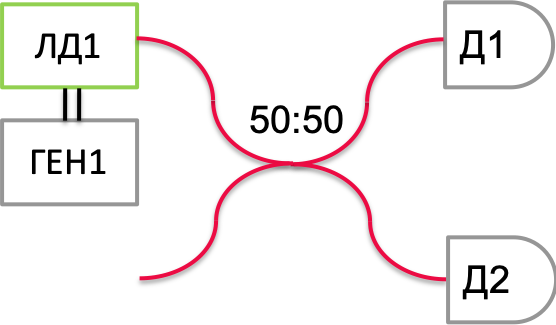
\includegraphics{Scheme_2.4.eps}
  \caption{Принципиальная оптическая схема эксперимента}
  \label{fig:Scheme_2.4}
\end{figure}


График зависимости представлен на рисунке \ref{fig:Beamsplitter}. Видно, что расхождение оставляет величину не превышающую 1 дБ. Соответственно, далее при проведении всех измерений производится корректировка на полученную величину. Таким образом учитывается неидеальность коэффициента деления используемого волоконно-оптического светоделителя 2х2. 


 \begin{figure}[ht]
  \centering
  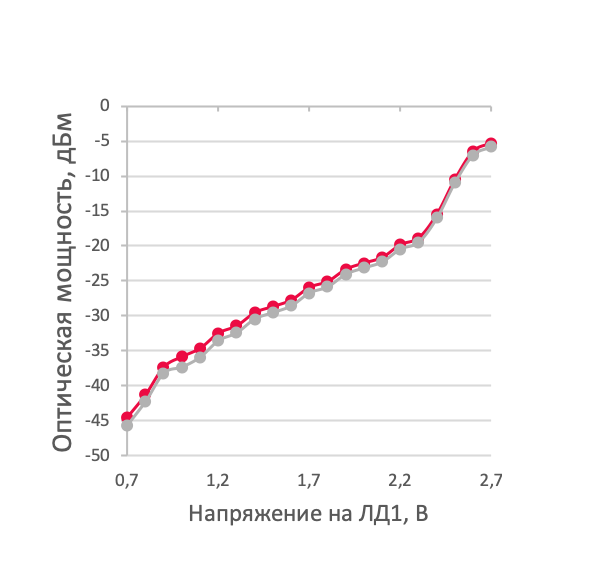
\includegraphics{Beamsplitter.png}
  \caption{Зависимость оптической мощности на двух выходах светоделителя 2х2 от величины напряжения на ЛД1}
  \label{fig:Beamsplitter}
\end{figure}
\pagebreak

%%%%%%%%%%%%%%%%%%%%%%%%%%%%%%%%%%%%%%%%%%%%%%%%%%%%%%%%%%%%%%%%%%%%%%%%%%%%%%%%%%%%%%%%%%%%%%%%%%%%%%%%%%%%%%%%%

\section{Определение величины постоянной оптической мощности, достаточной для выведения детектора из режима Гейгера} \label{sec:ch2/sec5}

На первом этапе выведения детектора из режима счета фотонов требуется определить необходимую и достаточную величину оптической мощности для <<ослепления>> детектора. Характерной особенностью и показателем успешного завершения первого этапа является отсутствие темновых срабатываний ДОФ в линейном режиме. Таким образом, задача сводится к тому, чтобы направить в детектор оптическое излучения в области спектральной чувствительности детектора, для простоты имитации действий злоумышленника это будет длина волны 1550~нм, и зафиксировать смену растущего количества отсчетов их полным отсутствием. На рисунке \ref{fig:Scheme_2.5} представлена оптическая схема эксперимента. 


 \begin{figure}[ht]
  \centering
  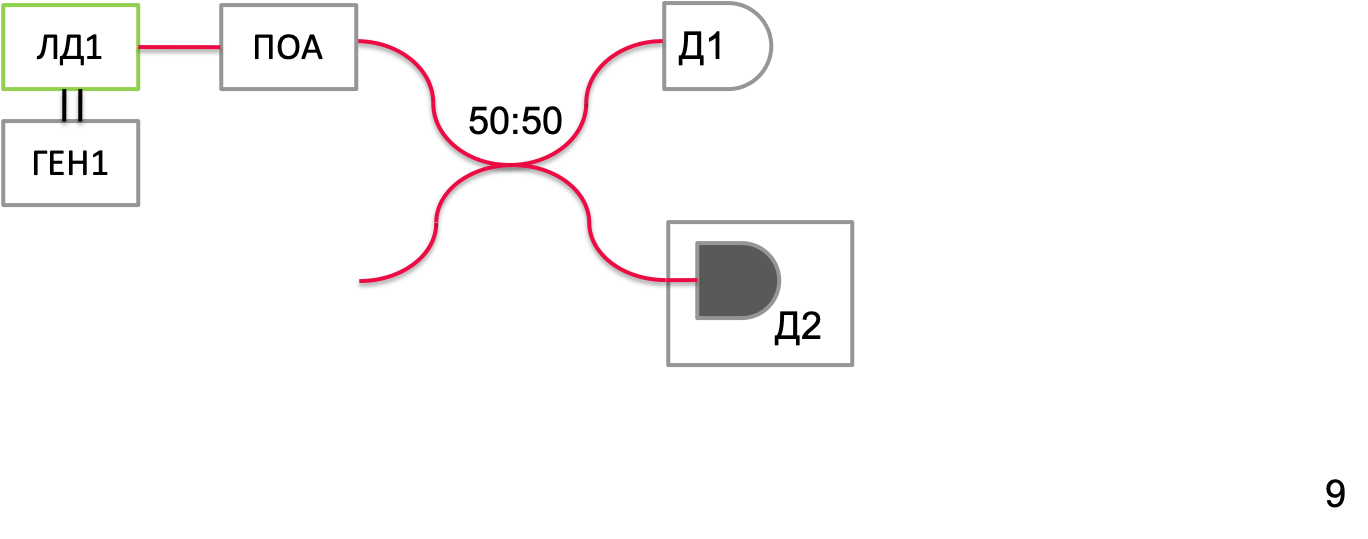
\includegraphics{Scheme_2.5.eps}
  \caption{Принципиальная оптическая схема эксперимента}
  \label{fig:Scheme_2.5}
\end{figure}

В качестве источника постоянного излучения применяется лазерный модуль с распределенной обратной связью (Alcatel 1905 LMI). Излучаемая длина волны - 1550~нм. Особенностями данного модуля так же являются узкая спектральная полоса порядка 2~МГц и встроенный оптический изолятор, предотвращающий попадание переотраженного излучения обратно в лазерный диод. 
 На лицевой панели индикатор количества отсчетов показывает все нули. 


Для детектора ID210 переход из режима Гейгера в линейный режим при штатных для системы квантовой коммуникации на боковых частотах настройках осуществляется при величине постоянной оптической мощности, превыщающей 24~нВт. Далее в оптических схемах ПОА исключен в связи с тем, что для изменения выходной мощности ЛД1 использовался генератор ГЕН1 с постоянным уровнем напряжения и шагом 0,1~В, как показано на \ref{fig:Beamsplitter}. При подаче постоянного напряжения 0,7~В излучаемая оптическая мощность оставляла 35~нВт, что в рамках данного исследования принималось за мощность, необходимую для <<ослепления>> детектора


%%%%%%%%%%%%%%%%%%%%%%%%%%%%%%%%%%%%%%%%%%%%%%%%%%%%%%%%%%%%%%%%%%%%%%%%%%%%%%%%%%%%%%%%%%%%%%%%%%%%%%%%%%%%%%%%%

\section{Подстройка оптического импульса под окно детектора одиночных фотонов} \label{sec:ch2/sec6}

Вторым этапом определения возможности контроля злоумышленником детектора на основе ЛФД является подстройка оптического импульса под окно ДОФ. Эта подстройка необходима для того, чтобы контролирующий оптический импульс лазерного источника злоумышленника точно приходил в момент ожидаемого прибытия фотона от блока отправителя. В ином случае, эффективность значительно снижается. В качестве источника контролирующих импульсов используется лазерный диод с распределенной обратной связью (DFB) <<Gooch \& Housego>> модели AA1401. Он излучает на длине волны 1550~нм с узкой спектральной полосой в 1~МГц. В качестве формирователя импульсов используется генератор ГЕН2 (Highland Technology P400). Импульсы с частотой 10~МГц и длительностью 0,5~нс подаются на ЛД2. Величина 10~МГц обусловлена минимальным возможным значением мертвого времени (deadtime) ДОФ, равным 100~нс. Это значит, что при подаче синхронизационной частоты в 100~МГц с блока отправителя системы квантовой коммуникации, окно детектирования будет открываться не чаще, чем 10~МГц. При помощи ГЕН2 вносится задержка по фазе импульса, подаваемого на ЛД2, с точностью до 1~пс. Синхронизационная частота 100~МГц имитируется средствами ГЕН2. На порт детектора <<Trigger>> подается указанная частота. При увеличении оптической мощности контролирующего импульса в ДОФ в линейном режиме увеличивается фототок и при некоторой величине превышает порог срабатывания компаратора. Таким образом на дисплее детектора отображаются отсчеты, количество которых возрастает с увеличением оптической мощности. Зафиксировав на некоторой величине мощность контролирующих импульсов требуется подстройка задержки этих импульсов при помощи ГЕН2. При изменении величины задержки наблюдается рабочая точка с глобальным максимумом. На рисунке \ref{fig:Scheme_2.6} продемонстрирована оптическая схема эксперимента.

 \begin{figure}[ht]
  \centering
  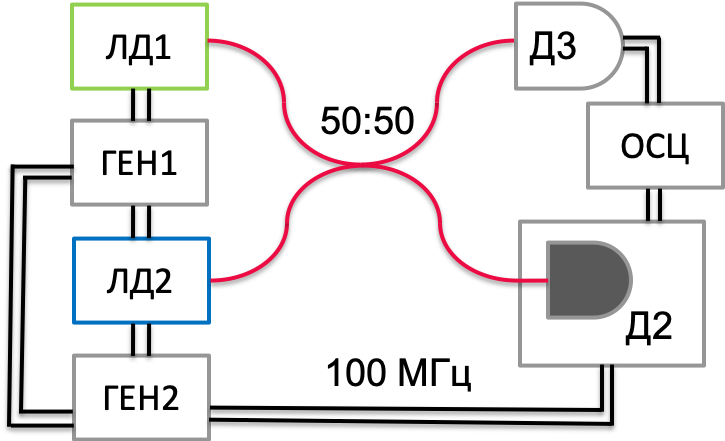
\includegraphics{Scheme_2.6.eps}
  \caption{Принципиальная оптическая схема эксперимента}
  \label{fig:Scheme_2.6}
\end{figure}

При этом в одном плече установлен оптоэлектронный преобразователь Д3 (LeCroy OE555), который подключен к осциллографу ОСЦ (LeCroy 820Zi) для наблюдения оптических импульсов. Также к этому осциллографу подключен выход детектора ID210 <<Detection 1>>, где можно наблюдать электрические импульсы срабатывания, и выход <<Gate>>, где можно наблюдать окна срабатывания. Полученная осциллограмма представлена на \ref{fig:LeCroy}. 

 \begin{figure}[ht]
  \centering
  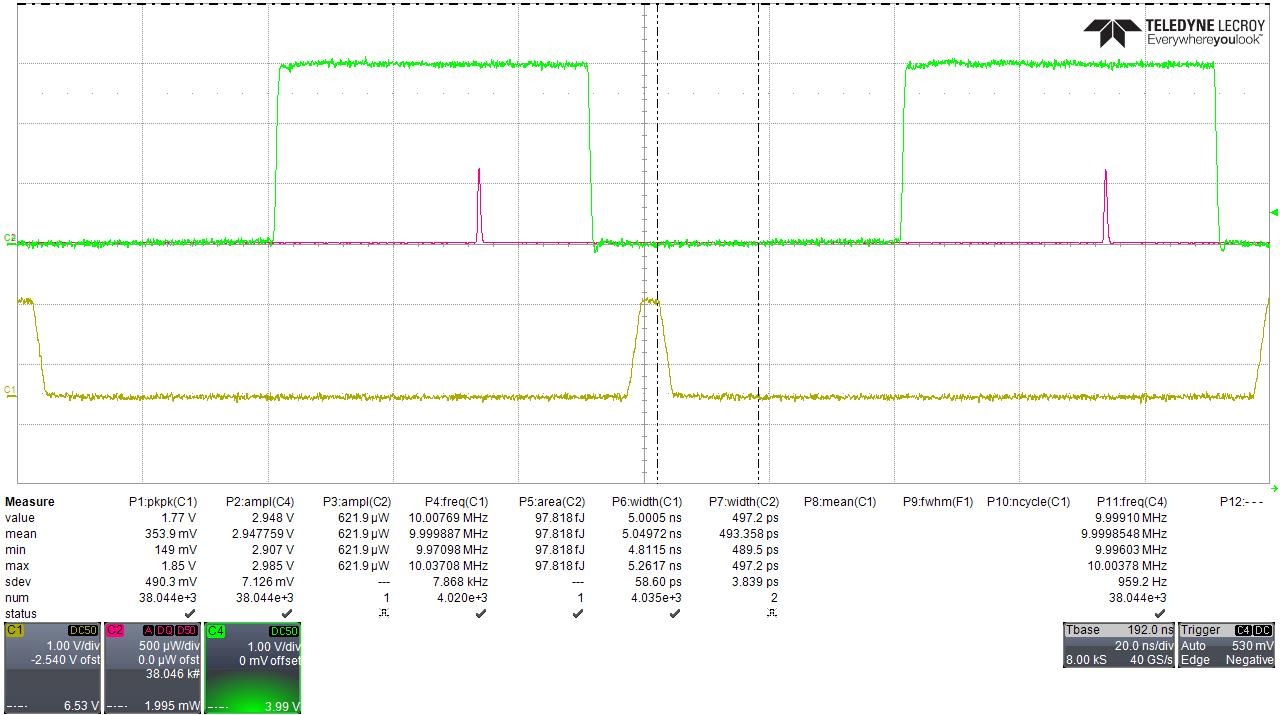
\includegraphics[scale=0.45] {LeCroy97.jpg}
  \caption{Осциллограмма с наблюдаемыми оптическими импульсами, окнами срабатываний детектора фотонов и опорной частотой}
  \label{fig:LeCroy}
\end{figure}



 \begin{figure}[ht]
  \centering
  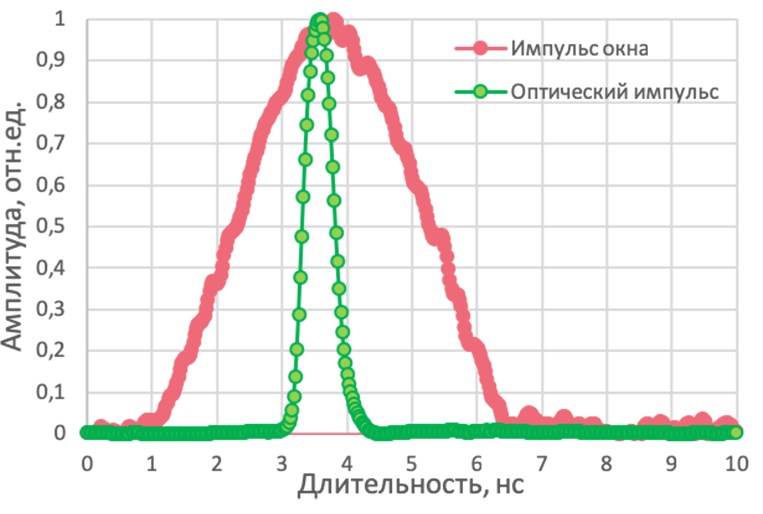
\includegraphics{images/optical pulse and gate.png}
  \caption{Осциллограммы контролирующего оптического импульса и окна срабатывания, скорректированные по фазе}
  \label{fig:optical_pulse_and_gate}
\end{figure}


\pagebreak
%%%%%%%%%%%%%%%%%%%%%%%%%%%%%%%%%%%%%%%%%%%%%%%%%%%%%%%%%%%%%%%%%%%%%%%%%%%%%%%%%%%%%%%%%%%%%%%%%%%%%%%%%%%%%%%%%


\section{Определение количества срабатываний детектора от величины мощности оптического излучения} \label{sec:ch2/sec7}


 \begin{figure}[ht]
  \centering
  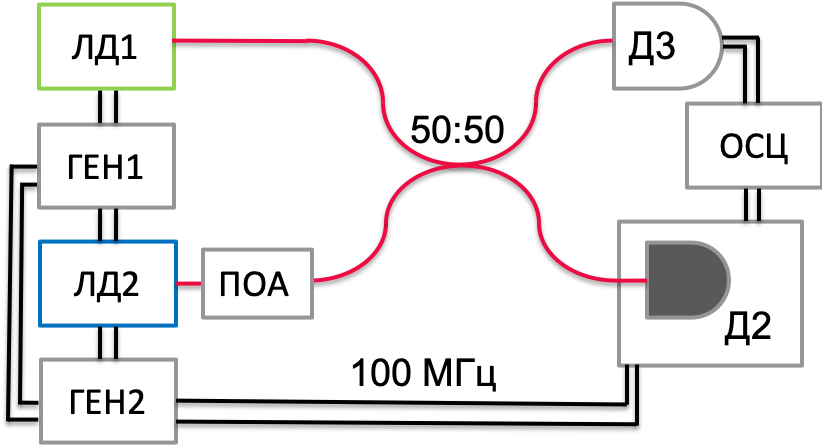
\includegraphics{Scheme_2.7.eps}
  \caption{Принципиальная оптическая схема эксперимента}
  \label{fig:Scheme_2.7}
\end{figure}


 \begin{figure}[ht]
  \centering
% хрень какая-то  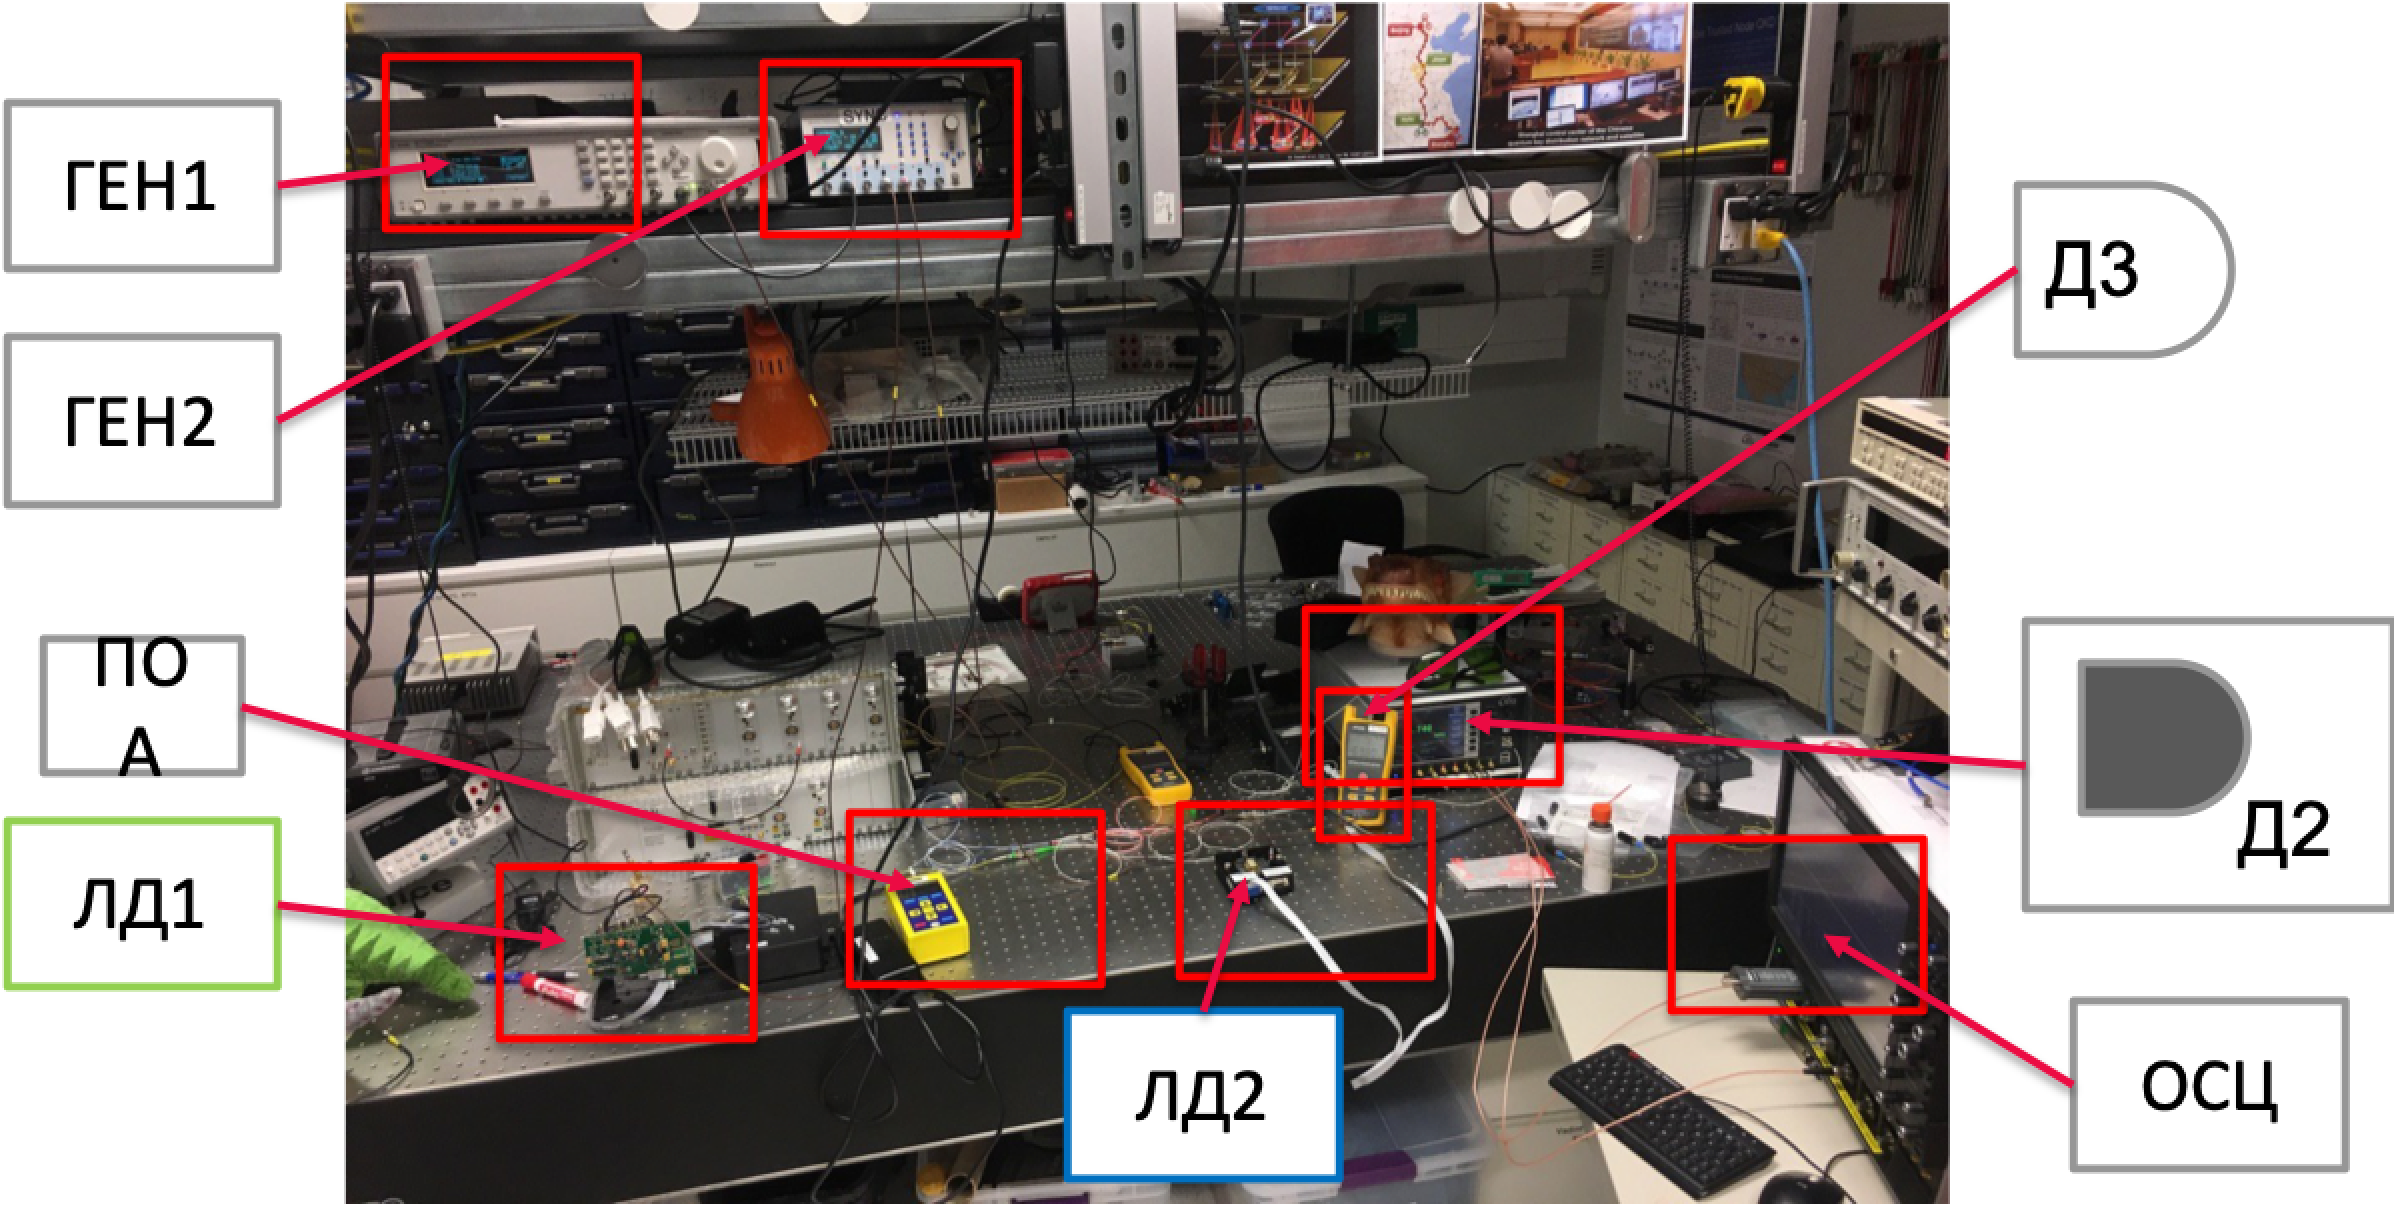
\includegraphics{blinding experimental setup02.png}
  \caption{Фотография экспериментального стенда}
  \label{fig:experimental_setup}
\end{figure}


 \begin{figure}[ht]
  \centering
  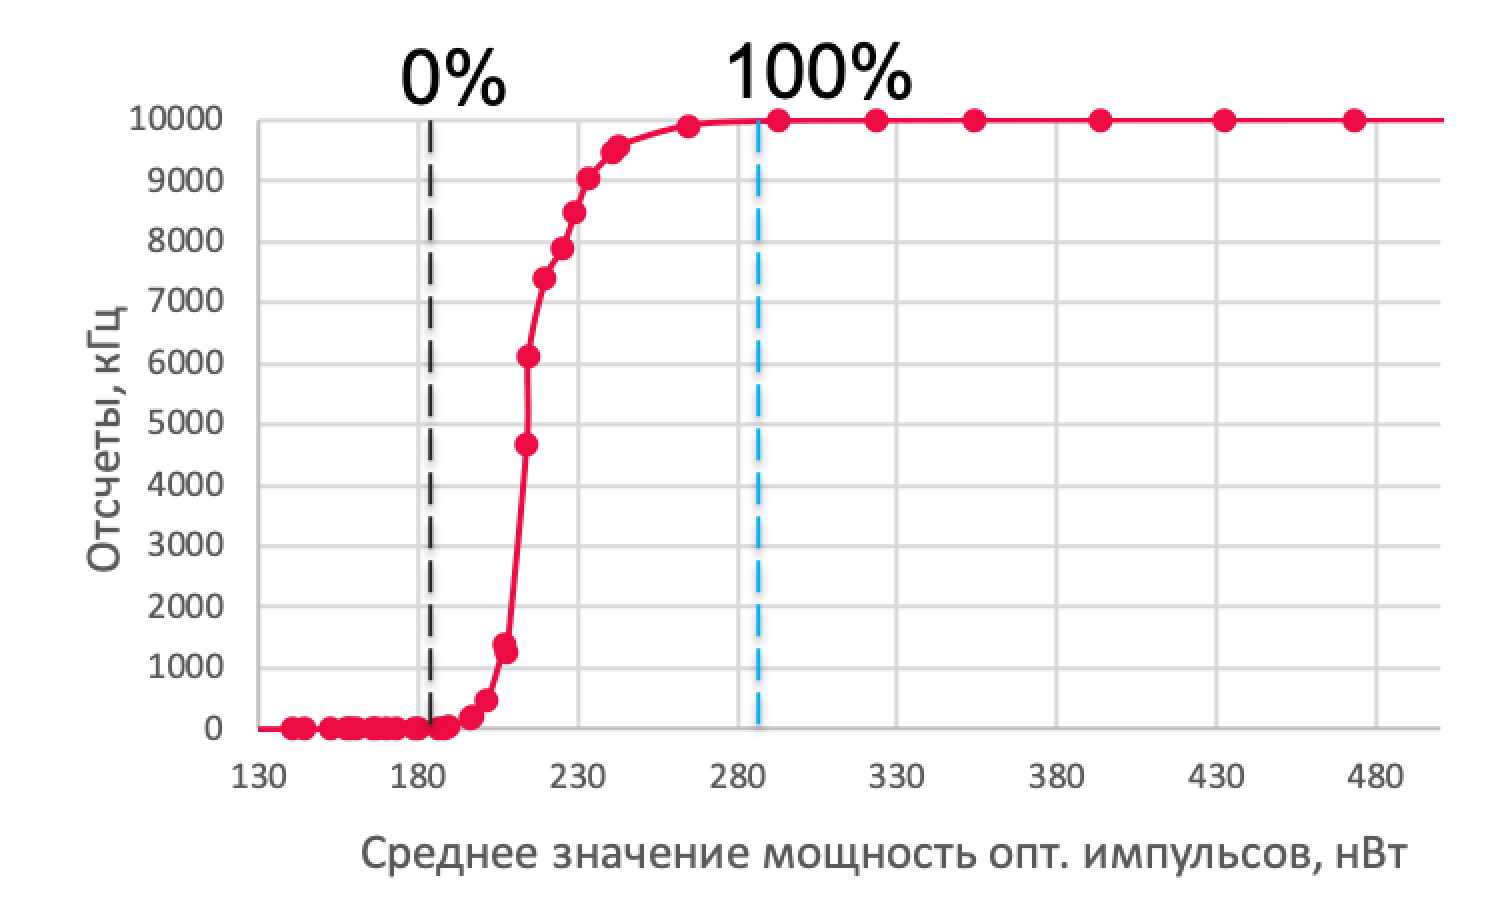
\includegraphics{35_nW.png}
  \caption{Зависимость количества отсчетов от величины оптической мощности контролирующего импульса}
  \label{fig:35_nW}
\end{figure}


\pagebreak
%%%%%%%%%%%%%%%%%%%%%%%%%%%%%%%%%%%%%%%%%%%%%%%%%%%%%%%%%%%%%%%%%%%%%%%%%%%%%%%%%%%%%%%%%%%%%%%%%%%%%%%%%%%%%%%%%


\section{Определение зависимости вероятности срабатывания детектора от величины мощности оптического излучения в квантовом канале} \label{sec:ch2/sec8}




\pagebreak
%%%%%%%%%%%%%%%%%%%%%%%%%%%%%%%%%%%%%%%%%%%%%%%%%%%%%%%%%%%%%%%%%%%%%%%%%%%%%%%%%%%%%%%%%%%%%%%%%%%%%%%%%%%%%%%%%


\section{Определение зависимости вероятности срабатывания детектора от величины энергии фотонов в импульсе} \label{sec:ch2/sec9}


%%%%%%%%%%%%%%%%%%%%%%%%%%%%%%%%%%%%%%%%%%%%%%%%%%%%%%%%%%%%%%%%%%%%%%%%%%%%%%%%%%%%%%%%%%%%%%%%%%%%%%%%%%%%%%%%%
\section{Атака с навязыванием ключа «поддельными» состояниями} \label{sec:ch2/sec10}


%%%%%%%%%%%%%%%%%%%%%%%%%%%%%%%%%%%%%%%%%%%%%%%%%%%%%%%%%%%%%%%%%%%%%%%%%%%%%%%%%%%%%%%%%%%%%%%%%%%%%%%%%%%%%%%%%
\section{Границы применимости атаки с навязыванием ключа} \label{sec:ch2/sec11}




%%%%%%%%%%%%%%%%%%%%%%%%%%%%%%%%%%%%%%%%%%%%%%%%%%%%%%%%%%%%%%%%%%%%%%%%%%%%%%%%%%%%%%%%%%%%%%%%%%%%%%%%%%%%%%%%%
\section{Оценка возможностей злоумышленника при атаке с выведением детектора из режима Гейгера для систем квантовой коммуникации на боковых частотах} \label{sec:ch2/sec12}



%%%%%%%%%%%%%%%%%%%%%%%%%%%%%%%%%%%%%%%%%%%%%%%%%%%%%%%%%%%%%%%%%%%%%%%%%%%%%%%%%%%%%%%%%%%%%%%%%%%%%%%%%%%%%%%%%
\section{Выводы по главе} \label{ch:ch2/sect13}
           % Глава 2
\chapter{Контрмера против атаки с навязыванием ключа} \label{ch:ch3}

%%%%%%%%%%%%%%%%%%%%%%%%%%%%%%%%%%%%%%%%%%%%%%%%%%%%%%%%%%%%%%%%%%%%%%%%%%%%%%%%%%%%%%%%%%%%%%%%%%%%%%%%%%%%%%%%%

\section{Атака с навязыванием ключа «поддельными» состояниями в системе квантовой коммуникации на боковых частотах} \label{sec:ch3/sec1}

В данной главе предлагается реализация атаки с <<поддельными>> состояниями на систему квантовой коммуникации на боковых частотах с используемым в приемном блоке детектором фотонов ID210. Как показали результаты исследования, изложенные во \ref{ch:ch2} главе, этот детектор подвержен выведению из режима Гейгера. Для осуществления успешной атаки между блоками легитимных отправителя и получателя располагается нелегитимный пользователь с аналогичным оборудованием. Всегда при рассмотрении возможностей злоумышленника предполагается, что они ограничены здравым смыслом и законами физики. Таким образом, принципиальная оптическая схема предлагаемой атаки представлена на рисунке \ref{fig:SCW_FSA}. 

 \begin{figure}[ht]
  \centering
  \includegraphics[scale=0.35]{scw-setup_FSA_rus1.pdf}
  \caption{Принципиальная оптическая схема предлагаемой атаки с <<поддельными состояниями>>}
  \label{fig:SCW_FSA}
\end{figure}

В состав подсистемы злоумышленника включена приёмная сторона, аналогичная получателю, и модифицированный под атаку блок отправителя. Первая часть подсистемы регистрирует срабатывания в соотвествии с протоколом. Применяемые квантовые состояния, которые привели к конструктивной интерференции, то есть за вычетом ошибок являются аналогичными по отношению к легитимному отправителю передаются в модифицированный блок отправителя. Модификация заключается в том, что в соотвествии с определёнными во \ref{ch:ch2} главе величинами, необходимыми для выведения детектора фотонов из режима Гейгера, источник формирует при помощи лазерного источника высокоинтенсивную несущую, затем в результате фазовой модуляции в спектре формируются боковые частоты, величина которых зависит от индекса модуляции. Весь спектр отправляется в приёмный блок, где в штатном режиме происходит повторная модуляция и интерференция сигналов на боковых частотах в зависимости от применяемых фазовых состояний. Затем отфильтровывается несущая частота, а боковые поступают на детектор одиночных фотонов. При этом мощность сигнала на боковых подбирается таким образом, чтобы её было достаточно для <<ослепления>> детектора и получения срабатывания в те моменты времени, когда злоумышленник отправляет известное, то есть совпавшее с легитимным отправителем, состояние. 


%%%%%%%%%%%%%%%%%%%%%%%%%%%%%%%%%%%%%%%%%%%%%%%%%%%%%%%%%%%%%%%%%%%%%%%%%%%%%%%%%%%%%%%%%%%%%%%%%%%%%%%%%%%%%%%%%
\section{Границы применимости атаки с навязыванием ключа} \label{sec:ch3/sec2}

Разберемся, чем обусловлены и ограничиваются параметры, которые модифицированная подсистема отправителя со стороны злоумышленника должна применять, чтобы успешно проводить предложенную атаку. 

В результате интерференции по аналогии со штатным режимом работы системы квантовой коммуникации с протоколом BB84 возможны 4 исхода, которые схематически представлены на рисунке \ref{fig:Palways}. Если разность фаз, применяемых при фазовой модуляции на стороне отправителя и получателя равна нулю, то интерференция конструктивна(КИ - <<конструктивная интерференция>>), то есть наблюдается усиление сигнала (при равных амплитудах  до четырехкратного увеличения). Если разность фаз равна $\pi$, то интерференция деструктивна (ДИ - <<деструктивная интерференция>>), то есть сигнал ослабляется до минимального уровня (шумов). Если используемые базисы не совпадают (НБ - <<несовпадение базисов>>), то разность фаз в обоих случаях равна $\pi/2$ и наблюдается половинный от максимального, соответствующего КИ, уровень мощности в классическом режиме, либо вероятность срабатывания 0,5 в квантовом режиме. 


 \begin{figure}[ht]
  \centering
  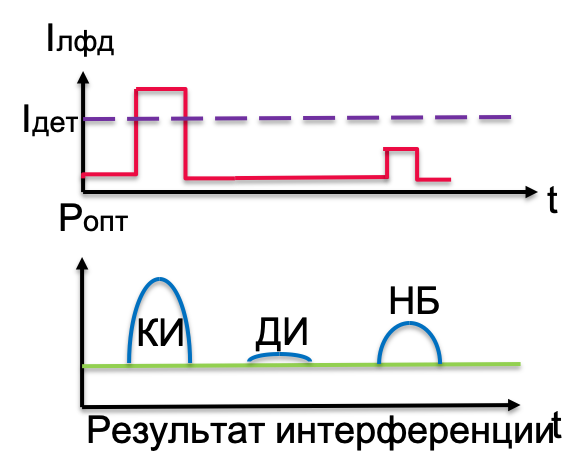
\includegraphics{Palways.png}
  \caption{Методика определения границ применимости}
  \label{fig:Palways}
\end{figure}


Стратегия злоумышленника максимально эффективна в том случае, когда легитимный пользователь с приёмником регистрирует срабатывания только в том случае, когда совпадение у отправителя и приёмной стороны злоумышленника было зафиксировано, а во все остальные моменты должно наблюдаться отсутствие срабатываний. Это условие будет автоматически выполняться в том случае, если фазовое состояние применяемое на приёмной стороне будет в противофазе с состоянием, пришедшим от модифицированной подсистемы злоумышленника, то есть будет наблюдаться ДИ. 

Однако, вариант с несовпадением базисов требует более внимательного рассмотрения. Для выполнения поставленного выше условия в случае несовпадения базисов требуется подобрать мощность контролирующих импульсов так, чтобы в результате интерференции порог срабатывания компаратора по току, протекающему в лавинном фотодиоде, не превысил уровень срабатывания, соответствущий току, необходимому для формирования импульса срабатывания. Это схематически представлено на рисунке \ref{fig:Palways}. \textit{Таким образом, накладывается ограничение сверху и снизу на оптическую мощность для контролирующих импульсов}. Чтобы приёмный блок не формировал срабатывания, не следует превышать величину оптической мощности $P_\text{никогда}$. А чтобы приёмный блок формировал состояния с единичной вероятностью, следует использовать мощность контролирующих оптических импульсов в пределах от $P_\text{никогда}$ до $P_\text{всегда\_предельное}$, которое равно удвоенному $P_\text{никогда}$:


\[
    \begin{cases}
     P < 2 \cdot P_\text{никогда} \\
     P \geqslant P_\text{всегда}
    \end{cases}
\]




Таким образом, детектор формирует импульс срабатывания только в случае совпадения используемых фазовых состояний, то есть конструктивной интерференции, и не должен формировать этот импульс при несовпадении базисов и деструктивной интерференции. Благодаря этому злоумышленник знает всю информацию о ключе, формируемом легитимными пользователями, а атака получила альтернативное название - <<навязывание ключа>>. Для разных оптических мощностей <<ослепления>> детектора фотонов определены границы применимости использования оптических мощностей контролирующих импульсов для формирования срабатывания и отсутствия срабатывания (рис. \ref{fig:Bounds}).  


 \begin{figure}[ht]
  \centering
  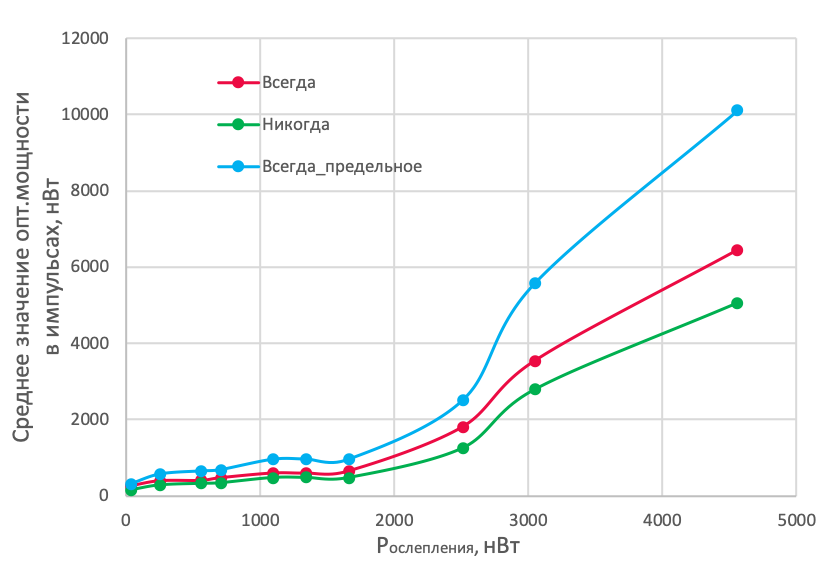
\includegraphics{Bounds.png}
  \caption{Границы применимости используемых оптических мощностей контролирующего импульса и засветки детектора}
  \label{fig:Bounds}
\end{figure}

%	\pagebreak

%%%%%%%%%%%%%%%%%%%%%%%%%%%%%%%%%%%%%%%%%%%%%%%%%%%%%%%%%%%%%%%%%%%%%%%%%%%%%%%%%%%%%%%%%%%%%%%%%%%%%%%%%%%%%%%%%
\section{Оценка возможностей злоумышленника при атаке с выведением детектора из режима Гейгера для систем квантовой коммуникации на боковых частотах} \label{sec:ch3/sec3}
 
 Приведем оценку необходимых параметров оптического излучения от модифицированной подсистемы злоумышленника для контроля детектора в приёмном блоке системы квантовой коммуникации на боковых частотах. Для этого воспользуемся полученными во \ref{ch:ch2} главе значениями. Известно, что блок получателя состоит из набора оптических компонентов (рис. \ref{fig:Bob}) со своими функциями и характеристиками, такими как вносимые потери и индекс модуляции.

 
 \begin{figure}[ht]
  \centering
  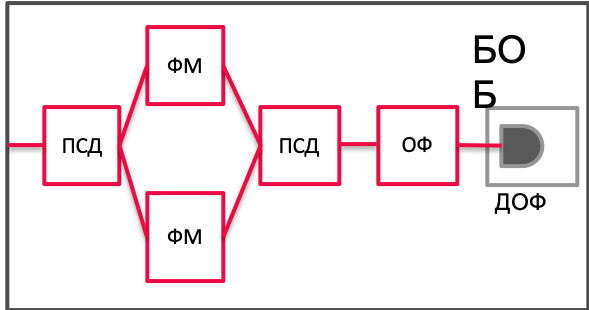
\includegraphics{Bob_scheme1.png}
  \caption{Принципиальная оптическая приемного модуля}
  \label{fig:Bob}
\end{figure}



Индекс модуляции, то есть соотношение энергии на центральной моде и на боковых равен 20:1. Таким образом, для того, чтобы детектор был ослеплен постоянной мощностью величиной в 35~нВт в спектре до фильтра должна быть величина в 20 раз больше.  Вносимые потери в блоке получателя составляют величину порядка 7 дБ. Расчеты представлены в таблице \ref{tab:blinding}.

 
 
\begin{table}
	\caption{\label{tab:blinding}Расчетные параметры для контроля детектора в системе квантовой коммуникации на боковых частотах.}
	\begin{tabular}[t]{c c c c}
	\hline\hline
	\makecell{Поддельное\\состояние\\злоумышленника\\мощность в...} & \makecell{Мощность для\\<<ослепления>> (нВт)} & $E_\text{всегда}$ (фДж) & $E_\text{никогда}$ (фДж) \\
	\hline
	\makecell{боковых после\\ фильтрации} & 35 & 25.8 & 15.4 \\
	\makecell{спектре перед\\ модуляцией} & 700 & 516 & 308 \\
	\makecell{спектре на входе\\ в приемный модуль} & 3056 & 2252 & 1345 \\
	\hline\hline
	\end{tabular}
\end{table}


\pagebreak

%%%%%%%%%%%%%%%%%%%%%%%%%%%%%%%%%%%%%%%%%%%%%%%%%%%%%%%%%%%%%%%%%%%%%%%%%%%%%%%%%%%%%%%%%%%%%%%%%%%%%%%%%%%%%%%%%

\section{Оптическая схема для противодействия атаке с <<ослеплением>> ДОФ} \label{ch:ch3/sec4}

В рамках данного исследования впервые в мире предлагается мера противодействия атакам с навязыванием ключа с использованием <<поддельных>> состояний с использованием преимуществ подхода к формированию квантовых состояний, а именно - вынесение квантового канала на боковые частоты фазомодулированного спектра.

Для определения попыток злоумышленника провести описанную выше атаку предлагается измерять интенсивность центральной оптической моды. Центральная мода отражается узкополосным фильтром на основе брэгговской решетки. Для того, чтобы её можно было измерить в схеме устанавливается волоконно-оптический циркулятор. Все излучение, которое после фазовых модуляторов в приемном блоке поступает на первый порт циркулятора направляется во второй порт на оптический фильтр. Отраженная центральная мода направляется в третий порт циркулятора. Для того, чтобы измерять центральную, которая, как показано в разделе \ref{sec:ch3/sec3}, должна быть порядка 700~нВт, предлагается использовать мониторный фотодиод. Так как. злоумышленника есть возможность подбирать интенсивность на центральной моде, то очевидным является то, что мониторный фотодиод, установленный на выходе с 3-го порта, можно также контролировать оптическими методами. Для того, чтобы избежать этого, предлагается использовать волоконно-оптическое зеркало, например широко доступное зеркало Фарадея, и пассивный оптический аттенюатор. Сам мониторный фотодиод предлагается устанавливать в 4-ом порту циркулятора. Таким образом, излучение с центральной модой поступает на 3-ий порт, проходит аттенюатор в прямом направлении, отражается от волоконного зеркала, проходит аттенюатор в обратном направлении и поступает на 4-й порт, где установлен мониторный фотодиод.         
 \begin{figure}[ht]
  \centering
  \includegraphics[scale=0.3]{scw-setup_Countermeasure.pdf}
  \caption{Принципиальная оптическая схема предлагаемой контрмеры против атаки с <<поддельными>> состояниями}
  \label{fig:countermeasure}
\end{figure}

\pagebreak

%%%%%%%%%%%%%%%%%%%%%%%%%%%%%%%%%%%%%%%%%%%%%%%%%%%%%%%%%%%%%%%%%%%%%%%%%%%%%%%%%%%%%%%%%%%%%%%%%%%%%%%%%%%%%%%%%
\section{Экспериментальная проверка контрмеры} \label{ch:ch3/sec5}

Для экспериментальной проверки предложенной контрмеры была собрана оптическая схема, воспроизводящая часть модифицированного подсистемы со стороны злоумышленника и блок получателя легитимного пользователя (рис. \ref{fig:Experimental_countermeasure}). 


 \begin{figure}[ht]
  \centering
  \includegraphics[scale=0.8]{Experimental_Countermeasure.pdf}
  \caption{Принципиальная оптическая схема предлагаемой контрмеры против атаки с <<поддельными>> состояниями}
  \label{fig:Experimental_countermeasure}
\end{figure}

Здесь стоит задача оценить работу в системе дополнительных элементов, введенных для активного мониторинга попыток злоумышленника вывести детектор одиночных фотонов и режима Гейгера постоянной оптической мощностью и контролировать срабатывания сильными оптическими импульсами. Для этих целей используются волоконно-оптический 4-ех портовый циркулятор, волоконное зеркало Фарадея и фиксированный аттенюатор розеточного типа с воздушным зазором на стыке феррул коннекторов зеркала и циркулятора. 

В модуле отправителя используются лазерный источник Л1, изолятор И, фазовый модулятор со встроенным поляризатором, подключенный электронике, программируемый оптический аттенюатор для регулировки выходной мощности с модуля. Управляющий сигнал представлен на рисунке \ref{fig:RF_sin_osc} и представляет из себя синус с частотой 4,8~ГГц. Амплитуда сигнала подбирается при помощи цифро-аналогового преобразователя ЦАП в пределах от 0 до 5~В таким образом, чтобы в результате модуляции 5~\% энергии несущей частоты распределялись на первой гармонике боковых частот.    


 \begin{figure}[ht]
  \centering
  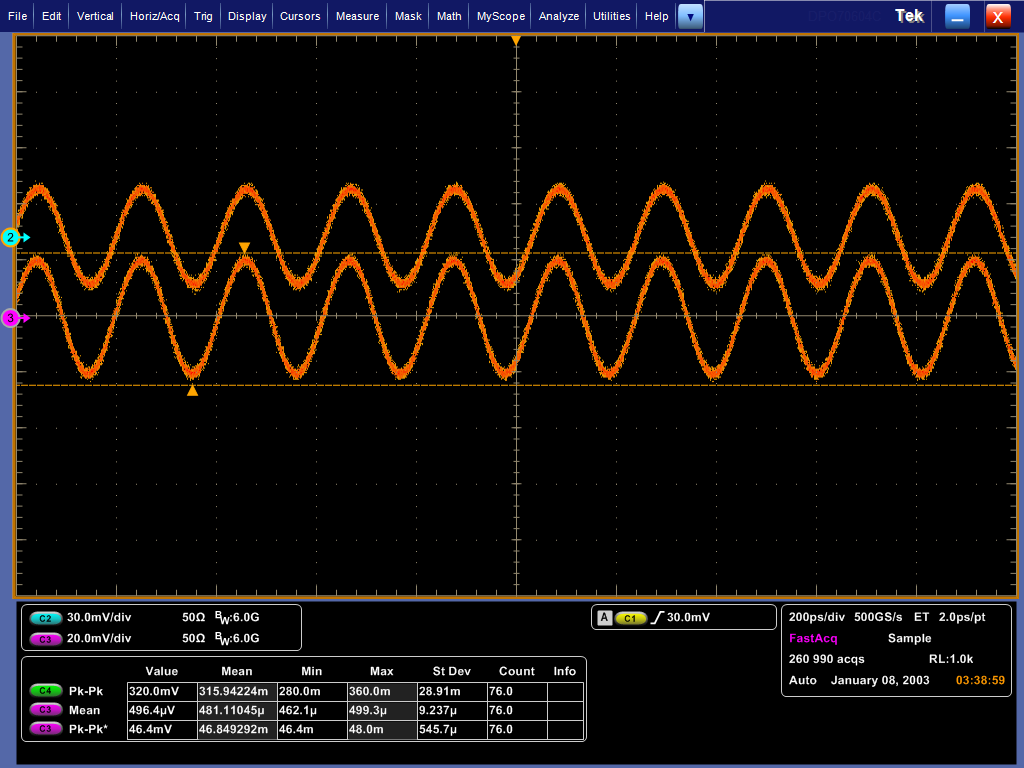
\includegraphics[scale=0.5]{sin_RF_mod_signal_constructive}
  \caption{Осциллограмма модулирующего сигнала в системе}
  \label{fig:RF_sin_osc}
\end{figure}


В приёмном модуле на 1-ый порт циркулятора Ц приходит излучение из модуля отправителя, которое с минимальными потерями не превышающими величину 1 дБ поступает на 2-ой порт с оптическим фильтром ОФ. Спектральная характеристика Л1 отстроена таким образом, чтобы центральная длина волны попадала в узкую полосу отражения ОФ, а боковые частоты проходили ОФ и поступали на детектор одиночных фотонов ДОФ. В отсутствие в схеме аттенюатора зафиксированы следующие величины оптических мощностей (табл. \ref{tab:Circulator}). Таким образом, видно, что порядок величин, полученных экспериментально согласуется с расчетными из раздела \ref{sec:ch3/sec3} в отсутствие подсистемы модуляции в приёмном блоке. 


\begin{table}
	\caption{\label{tab:Circulator}Измеренные параметры при выведении детектора из режима счета фотонов в системе квантовой коммуникации.}
	\begin{tabular}[t]{c c c}
	\hline\hline
	\makecell{Мощность в...} & \makecell{Значение мощности (нВт)} & Значение мощности (дБм)  \\
	\hline
	\makecell{спектре на входе\\ в приемный модуль} & 2440 & -26.12 \\
	\makecell{боковых после\\ фильтрации} & 114.8 & -39.42 \\
	\makecell{отраженной от фильтра\\ центральной} & 1127 & -29.48  \\
	\makecell{на входе\\в мониторный диод} & 830 & -30.9  \\	
	\hline\hline
	\end{tabular}
\end{table}


\pagebreak
%%%%%%%%%%%%%%%%%%%%%%%%%%%%%%%%%%%%%%%%%%%%%%%%%%%%%%%%%%%%%%%%%%%%%%%%%%%%%%%%%%%%%%%%%%%%%%%%%%%%%%%%%%%%%%%%%
\section{Динамика оптической мощности на мониторном фотодиоде}\label{ch:ch3/sec6}

Благодаря граничным условиям на величину контролирующих оптических импульсов:

\[
    \begin{cases}
     P < 2 \cdot P_\text{никогда} \\
     P \geqslant P_\text{всегда}
    \end{cases}
\]

характеристикам устройств в приёмном блоке системы квантовой коммуникации, можно произвести количественную оценку требуемого диапазона чувствительности мониторного фотодиода и величину вносимого затухания аттенюатора, включенного в схему для защиты мониторного фотодиода от засветки злоумышленником. \textit{Для практических применений эта оценка является одним из весомых результатов исследования, так как позволяют достаточно простым способом с использованием преимуществ метода формирования квантовых состояний на боковых частотах отслеживать попытки злоумышленника по воздействию на детектор фотонов и навязыванию ключа легитимным пользователям}. 

На рисунке \ref{fig:Watchdog_photodiode} представлены две зависимости: нижний предел -- величина оптической мощности, которая требуется для выведения детектора фотонов из режима Гейгера и является минимальной необходимой для проведения успешной атаки злоумышленником; верхняя граница - величина оптической мощности, которая получена исходя из параметров приёмного модуля системы квантовой коммуникации и ограничения сверху на величину оптической мощности контролирующих импульсов. Минимальный уровень в соотвествии с расчетом составляет 0.7~мкВт, а максимальный - величину порядка 300~мкВт (в рамках данного исследования), однако на деле ограничен пороговой величиной ЛФД внутри ДОФ, при достижении которой ток становится слишком большим и диод сгорает, выводя из строя всё устройство. Типичной величиной являются единицы и десятки милливатт. 


С учётом данной зависимости можно оценить величину ослабления в фиксированном аттенюаторе, которой будет достаточно для защиты мониторного фотодиода от засветки, и при этом не потребуются дополнительные меры по расширению динамического диапазона чувствительности к входной оптической мощности в сторону увеличения, так как при оптических мощностях ниже единиц нановатт погрешность измерений становится достаточно высокой.   

Исходя из этого, величины аттенюации в 10~дБ достаточно, так как отраженная центральная на выходе с 3-го порта циркулятора прохоит через ослабляющий элемент в первый раз, а затем после отражения от зеркала во второй раз. Результирующее ослабление на 20~дБ, или в 100 раз, снизит минимальный уровень мощности на центральной частоте, которого достаточно для выведения детектора из режима счета фотонов, до величины порядка 7~нВт, что удовлетворяет требованиям, описанным выше. Максимальный уровень (в рамках данного исследования) снизится при этом примерно до 3~мкВт. 

 \begin{figure}[ht]
  \centering
  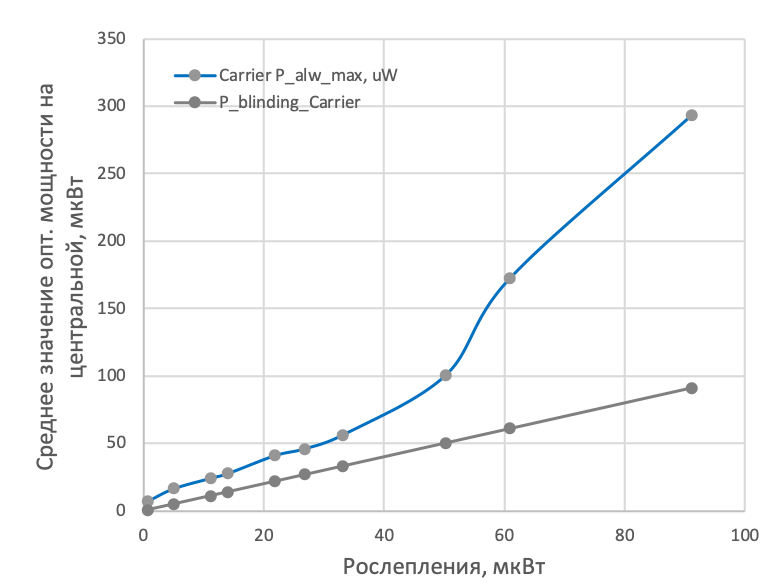
\includegraphics{images/Watchdog_photodiode.png}
  \caption{Динамика и границы оптической мощности на мониторном фотодиоде}
  \label{fig:Watchdog_photodiode}
\end{figure}


\pagebreak
%%%%%%%%%%%%%%%%%%%%%%%%%%%%%%%%%%%%%%%%%%%%%%%%%%%%%%%%%%%%%%%%%%%%%%%%%%%%%%%%%%%%%%%%%%%%%%%%%%%%%%%%%%%%%%%%%
\section{Выводы по главе} \label{ch:ch3/sec7}


В \ref{ch:ch3} главе показано, что измерение величины оптического излучения на несущей частоте, отраженного от оптического фильтра, при помощи мониторного фотодиода в приемном блоке системы квантовой коммуникации на боковых частотах в диапазоне от 7 нВт до 2,93 мкВт с применением дополнительных мер в виде пассивного оптического аттенюатора номиналом 10 дБ для его защиты позволяет противостоять атаке с выведением детектора одиночных фотонов из режима Гейгера и навязыванием ключа нелегитимным пользователем. 
             % Глава 3
\chapter{Многомодовые когерентные состояния и их интерференция}  \label{ch:ch4}
\section{Квантовое описание когерентного состояния} \label{sec:ch4/sec1}

Термин \textit{когерентное состояние} был введен Р. Дж. Глаубером. в 1963 г. Оно не совсем соотносится с классическим термином когерентность, но имеет отношение к специальному типу чистых квантово-механических состояний светового поля, соответствующего одиночной моде резонатора. Когерентное состояние определяется, как суперпозиция Фоковских состояний, то есть состояний числа фотонов. 


\begin{equation}
	\begin{aligned}
		|\alpha \rangle = \sum_{n=0}^\infty   |  \rangle,
	\end{aligned}
\end{equation}

Комплексное число $ \alpha $	определяется среднее число фотонов, которое равно квадрату модуля, и фазой когерентного состояния. Из выражения видно, что вероятность нахождения n фотонов в когерентном состоянии определяется, как показано в уравнении. 

\begin{equation}
	\begin{aligned}
		|\alpha \rangle = \sum_{n=0}^\infty   |  \rangle,
	\end{aligned}
\end{equation}

где - это среднее число фотонов. Видно, что когерентное состояние подчиняется распределению Пуассона. Когерентное состояние имеет свойства близкие классическим состояниям света. Отдельный случай когерентного состояния - это когда =0. Оно называется вакуумным состоянием с нулевым числом фотонов. Однако, в таком случае все равно наблюдаются квантовые флуктуации электрического и магнитного полей, которые иногда называют вакуумным шумом. 


%	\pagebreak

%%%%%%%%%%%%%%%%%%%%%%%%%%%%%%%%%%%%%%%%%%%%%%%%%%%%%%%%%%%%%%%%%%%%%%%%%%%%%%%%%%%%%%%%%%%%%%%%%%%%%%%%%%%%%%%%%
\section{Когерентные состояния после прохождения светоделителя} \label{ch:ch4/sec2}
 
Рассмотрим следующую систему: на вход светоделителя 2х2 подается когерентное состояние $| \psi \rangle_{\alpha}$, формируемое лазерным источником Л1. На второй порт поступает вакуумное состояние $| \psi \rangle_{\beta}$. При этом:

\begin{equation}
	| \psi \rangle_{\alpha} = | \alpha_{0} e^{i\phi_{0}k} \rangle \\
\end{equation}

\begin{equation}
	| \psi \rangle_{\beta} = | vac \rangle \\
\end{equation}


На обоих выходах светоделителя будет состояние  $| \frac{\alpha_{0}}{\sqrt{2}} \rangle$, поступающее на электро-оптические фазовые модуляторы ФМ1 и ФМ2. В результате фазовой модуляции состояние преобразуется в $| \alpha_{1} \rangle$ и $| \alpha_{2} \rangle$. 


 \begin{figure}[ht]
  \centering
  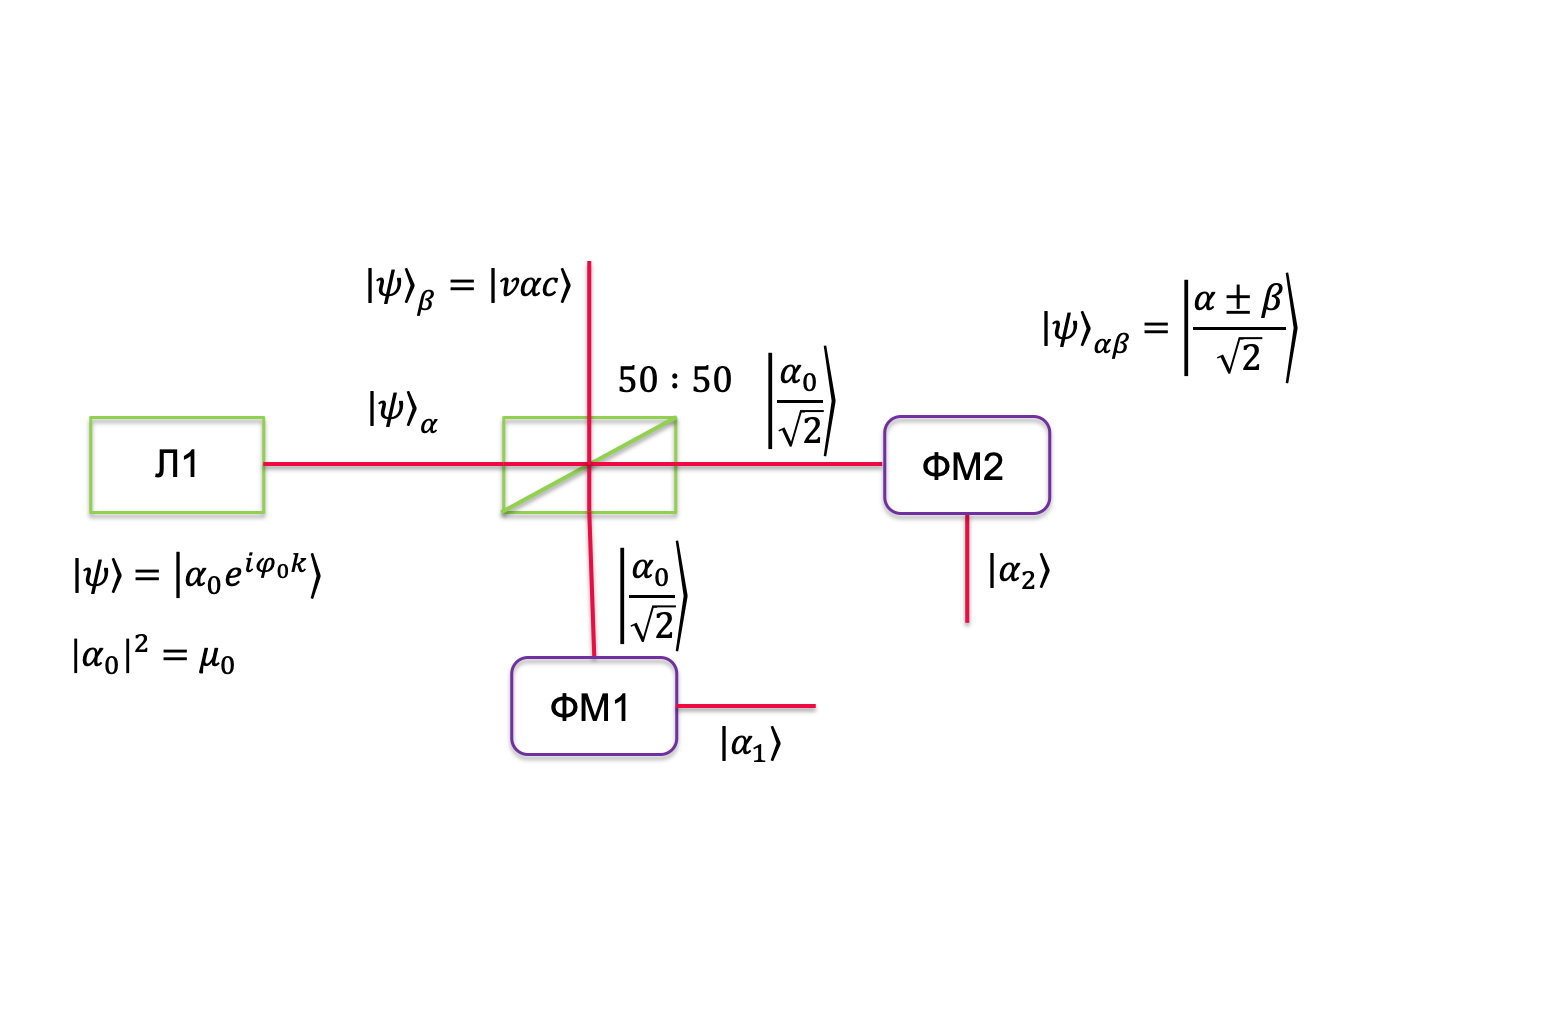
\includegraphics[scale=0.6]{Coherent_states_beamsplitting.png}
  \caption{Принципиальная схема наблюдения динамики когерентных состояний}
  \label{fig:Coherent_states_beamsplitting}
\end{figure}

\pagebreak

%%%%%%%%%%%%%%%%%%%%%%%%%%%%%%%%%%%%%%%%%%%%%%%%%%%%%%%%%%%%%%%%%%%%%%%%%%%%%%%%%%%%%%%%%%%%%%%%%%%%%%%%%%%%%%%%%
\section{Когерентные состояния после модуляции} \label{ch:ch4/sec3}

Отличительно особенностью систем квантовой коммуникации на боковых частотах модулированного излучения является генерация многомодовых когерентных состояний на разных оптических модах, зависящих от частоты модулирующего сигнала, как показано на рисунке \ref{fig:multimodes}. 

 \begin{figure}[ht]
  \centering
  \includegraphics[scale=0.6]{Modes_rus.pdf}
  \caption{Принципиальная схема генерации боковых частот}
  \label{fig:multimodes}
\end{figure}


Определим приготовленные состояния. Входное (немодулированное) состояние на стороне модулятора отправителя (Алиса) и получателя (Боб) (далее именуемые, как $A$ or $B$) определяется, как $|\sqrt{\mu_0}\rangle_0\otimes|\mathrm{vac}\rangle_{SB}$, где $|\mathrm{vac}\rangle_{SB}$ это вакуумное состояние на боковых и $|\sqrt{\mu_0}\rangle_0$ это когерентное состояние несущей частоты с амплитудой, определенной средним числом фотонов $\mu_0$ в окне пропускания. формируемая когерентным монохроматическим излучением с оптической частотой $\omega$. Фаза несущей волны принимается как опорная и все остальные фазы считаются по отношению к ней. Электро-оптический фазовый модулятор (с частотой колебаний микроволнового поля $\Omega$ и её фазой $\varphi_A$ или $\varphi_B$) перераспределяет энергию между взаимодействующими модами (поле на выходе модулятора приобретает боковые частоты $\omega_k=\omega+k\Omega$, ограничим рассматриваемый нами случай $2S$ боковыми частотами и пусть целое число $k$ мод ограничено пределами $-S\le k\le S$), так, что состояние поля на выходе модулятора - это многомодовое когерентное состояние: 
%
\begin{equation}\label{phi}
|\psi_0(\varphi_j)\rangle = \bigotimes_{k=-S}^S|{\alpha_k(\varphi_j)}\rangle_k,
\end{equation}
%
где $j$ это и $A$, и $B$ (определяющее Алису или Боба), а амплитуды имеют следующий вид: 
%
\begin{equation}\label{alpha}
\alpha_k(\varphi_j)=\sqrt{\mu_0}d^S_{0k}(\beta)e^{i\varphi_jk},
\end{equation}
%
и $d^S_{nk}(\beta)$ это d-функция Вигнера, взятая из квантовой теории углового момента \cite{varshalovich1988quantum}, $\beta$ определяется индексом модуляции $m$, который без учета дисперсии в среде модулятора можно выразить: 
%
\begin{equation}\label{betam}
\cos{({\beta})}=1-\frac{1}{2}{\left(\frac{m}{S+0.5}\right)^2},
\end{equation}
где $S$ количество взаимодействующий мод, принимаемое очень большим. 

\pagebreak

%%%%%%%%%%%%%%%%%%%%%%%%%%%%%%%%%%%%%%%%%%%%%%%%%%%%%%%%%%%%%%%%%%%%%%%%%%%%%%%%%%%%%%%%%%%%%%%%%%%%%%%%%%%%%%%%%
\section{Результат интерференции когерентных состояний после модуляции} \label{ch:ch4/sec4}

После распространения по квантовому каналу амплитуда когерентного состояния ослабляется и имеет следующий вид:

\begin{equation}
\sqrt{\eta_c}\alpha_k(\varphi_j)=\sqrt{\mu_0\eta_c}d^S_{0k}(\beta)e^{i\varphi_jk},
\end{equation}


где $\eta_c$ оптическое пропускание канала. На втором светоделителе состояния преобразуются в следующий вид: 

\begin{align}\label{states}
\Big|\frac{\alpha_A \pm \alpha_Be^{i\varphi_0}}{2}\Big\rangle_{1,2} &= \bigotimes_{k=-S}^{S}\Big|\sqrt{\frac{\mu_0\eta_c}{2}}d_{0k}^{S}(\beta)\left(e^{i\varphi_Ak}\pm e^{i(\varphi_Bk+\varphi_0)}\right)\Big\rangle_k.
\end{align}
Выражение с плюсом определяется, как состояние на первом выходе второго светоделителя (нижний индекс $1$), а выражение с минусом как состояние на втором выходе второго светоделителя (нижний индекс  $2$). 
 
\begin{figure}[ht]
 \centering
  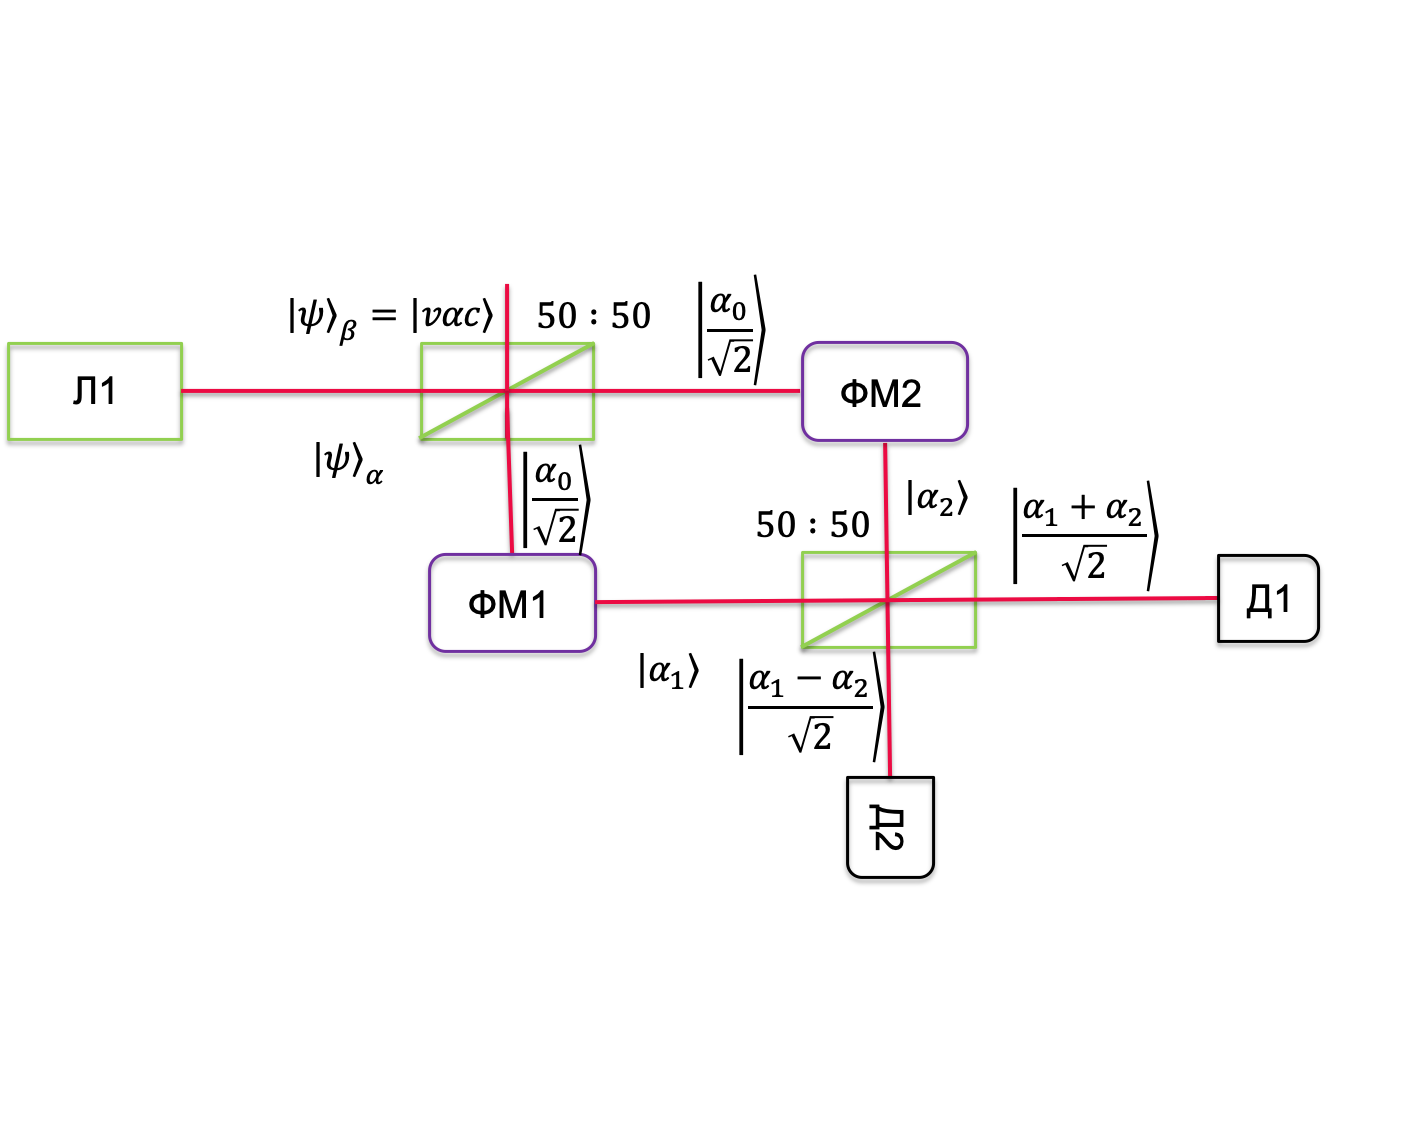
\includegraphics[scale=0.6]{Coherent_state_beamsplitting2.png}
  \caption{Принципиальная схема наблюдения динамики когерентных состояний}
  \label{fig:Coherent_states_beamsplitting2}
\end{figure}

\pagebreak

%%%%%%%%%%%%%%%%%%%%%%%%%%%%%%%%%%%%%%%%%%%%%%%%%%%%%%%%%%%%%%%%%%%%%%%%%%%%%%%%%%%%%%%%%%%%%%%%%%%%%%%%%%%%%%%%%
\section{Зависимость результата интерференции от разности фаз когерентных состояний} \label{ch:ch4/sec5}

После подстройки относительной фазы оптических сигналов в двух плечах, наблюдается интерференция этих состояний на втором светоделителе ($СД2$). Описание состояний на выходах светоделителя дано в уравнении~\ref{states}. Далее предполагается, что относительная фазовая отстройка оптических импульсов равна $\phi_0\approx0$. Если разность фаз между радиочастотными модулирующими сигналами Алисы и Боба равна нулю ($\Delta\varphi=0$) весь спектр идет в одно выходное плечо светоделителя $СД2$, в ином случае, четные моды спектра, включая центральную, идут в то же плечо, а нечетные идут во второе плечо. В случае $\Delta\varphi=0$, требуется спектральное разделение центральной частоты и боковых в приёмном блоке, так как кодирование квантовых состояний происходит на боковых частотах. Следует учитывать, что при использовании малого среднего числа фотонов в импульсе, значительный вклад в многомодовых состояниях вносят только первая пара боковых частот. Случай, при котором $\Delta\varphi=\pi$, является нетривиальным. Многомодовое состояние разделяется на $СД2$ и центральная мода (и все четные) идут в первое плечо, а все нечетные (первые боковые частоты вносят наибольший вклад в результирующий сигнал) идут во второе плечо, как показано на рисунке \ref{fig:Interference_result}. Таким образом, можно отказаться от спектрального разделения при помощи оптического фильтра в одном из выходных плечей приёмного узла. Показателем хорошей подстройки по фазе оптических импульсов является постоянный высокий уровень на центральной частоте в первом плече (на $Д2$).  


\begin{figure}[ht]
 \centering
  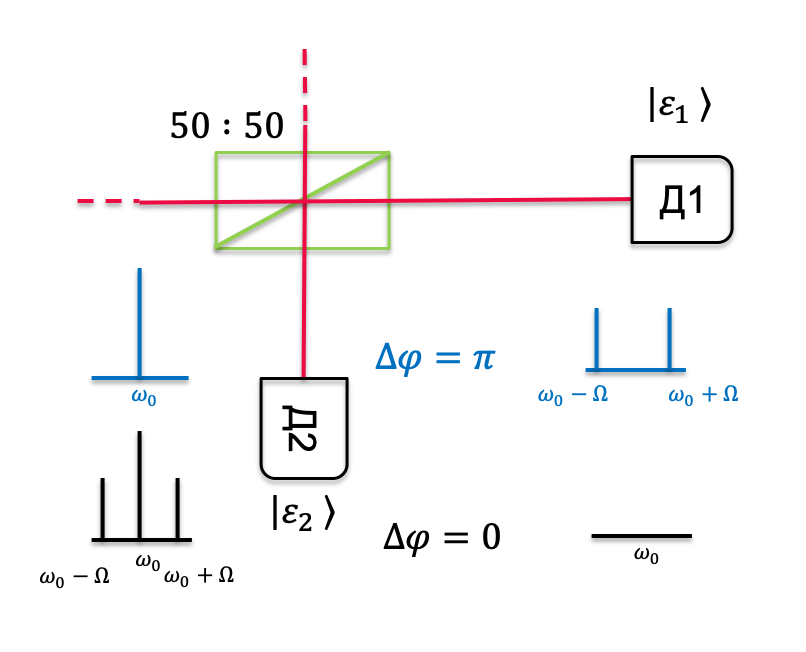
\includegraphics[scale=0.9]{Interference_result.png}
  \caption{Принципиальная схема наблюдения результата интерференции когерентных состояний}
  \label{fig:Interference_result}
\end{figure}

\pagebreak

%%%%%%%%%%%%%%%%%%%%%%%%%%%%%%%%%%%%%%%%%%%%%%%%%%%%%%%%%%%%%%%%%%%%%%%%%%%%%%%%%%%%%%%%%%%%%%%%%%%%%%%%%%%%%%%%%
\section{Протокол системы квантовой рассылки ключа, устойчивый к атакам на измерительное оборудование} \label{ch:ch4/sec6}

Основываясь на полученных результатах можно сформулировать протокол для системы квантовой коммуникации, использующей многомодовые когерентные состояния, с недоверенным измерительным узлом (рис. \ref{fig:Protocol}. Для простоты приведем пример с использованием только двух фазовых состояний по аналогии с протоколом B92. Алиса случайным образом выбирает одно фазовое состояние из двух возможных <<$0$>> или <<$\pi$>>. Боб независимо от Алисы тоже случайным образом выбирает одно из двух фазовых состояний. В результате интерференции многомодовых когерентных состояний можно наблюдать 4 различных варианта, в зависимости от разности фаз, выбранных Алисой и Бобом.  При этом на недоверенном узле регистрации будет происходить спектральное разделение, описанное в разделе \ref{sec:ch4/sec5}, так что на $Д1$ и $Д2$ будут поступать боковые частоты. Злоумышленник при этом имеет полный доступ к недоверенному измерительному узлу и может фиксировать себе оглашенный результат срабатываний одного из детекторов. Положим, что нас интересует только случай, при котором разность фаз между $А$ и $Б$ равна $\pi$. Преимущество этого случая в том, что за счет спектрального разделения в результате интерференции в плечо с детектором $Д1$ всегда будут идти только боковые и никогда не будет идти центральная мода, а значит можно исключить из оптической схемы этого плеча оптический фильтр, согласование которого с фильтром в другом плече -- достаточно трудная инженерная задача. Таким образом, при просеивании остаются только те биты, которые соответствуют отсчетам на $Д1$, при этом для корреляции между битами Алисы и битами Боба последний должен сделать смену бита на противоположный (так называемый <<bitflip>>).  

\begin{figure}[ht]
 \centering
  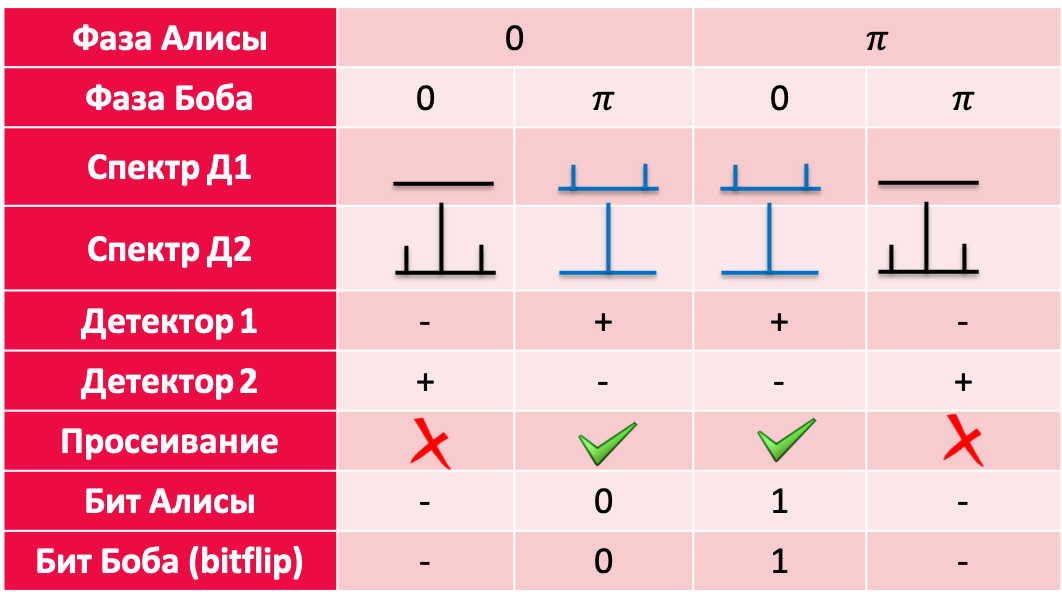
\includegraphics[scale=0.9]{Protocol.png}
  \caption{Протокол}
  \label{fig:Protocol}
\end{figure}


\pagebreak

%%%%%%%%%%%%%%%%%%%%%%%%%%%%%%%%%%%%%%%%%%%%%%%%%%%%%%%%%%%%%%%%%%%%%%%%%%%%%%%%%%%%%%%%%%%%%%%%%%%%%%%%%%%%%%%%%
\section{Выводы по главе} \label{ch:ch4/sec7}


В \ref{ch:ch4} главе показано, что метод квантовой коммуникации на боковых частотах позволяет реализовывать протокол, устойчивый к контролю нелегитимным пользователем измерительного оборудования. 
 
\pagebreak

           % Глава 4
\chapter{Экспериментальное исследование параметров устройства квантовой коммуникации с недоверенным приемным узлом} \label{ch:ch5}
\section{Интерференция сигналов на боковых частотах фазомодулированного излучения} \label{sec:ch5/sec1}

Для проверки концепции была собрана оптическая схема, представленная на рисунке \ref{fig:RF_sin}. Для простоты использовался только один источник излучения, сигнал на выходе которого делился светоделителем 50:50 $СД1$. Такой подход позволяет имитировать случай, когда у Алисы и Боба хорошо скоррелированные источники излучения. В данном эксперименте применялся лазер с распределенной обратной связью Л1 (TTX1994 Neophotonics), отличительными особенностями которого являются очень узкая ширина спектральной линии порядка 100~кГц и широкий диапазон перестройки длин волн (от 1530~нм до 1565,5~нм) с высокой степенью точности (20~пм). Выходная мощность при этом составляла 10~мВт. Однако, это значение зависит от глубины динамического диапазона перестраиваемого оптического аттенюатора ПОА и суммарных потерь, вносимых элементами Алисы или Боба, так как результирующая мощность сигнала на боковых частотах должна не превышать величину 2,56~пВт, соответствующую среднему числу фотонов в импульсе 0,2 при частоте смены состояний 100~Мгц.   

Из-за чувствительности резнатора внутри лазера с распределенной обратной связью к обратному относительно выходного оптическому излучению, то есть переотражениям и рассеиванию сигналов, в оптической схеме применяется волоконный изолятор И на основе эффекта Фарадея с величиной изоляции порядка 50~дБ. Для перевода системы в однофотонный режим применяется ПОА с достаточной малым шагом перестройки 0,05 дБ и большим динамическим диапазоном величиной 60~дБ.  

 \begin{figure}[ht]
  \centering
  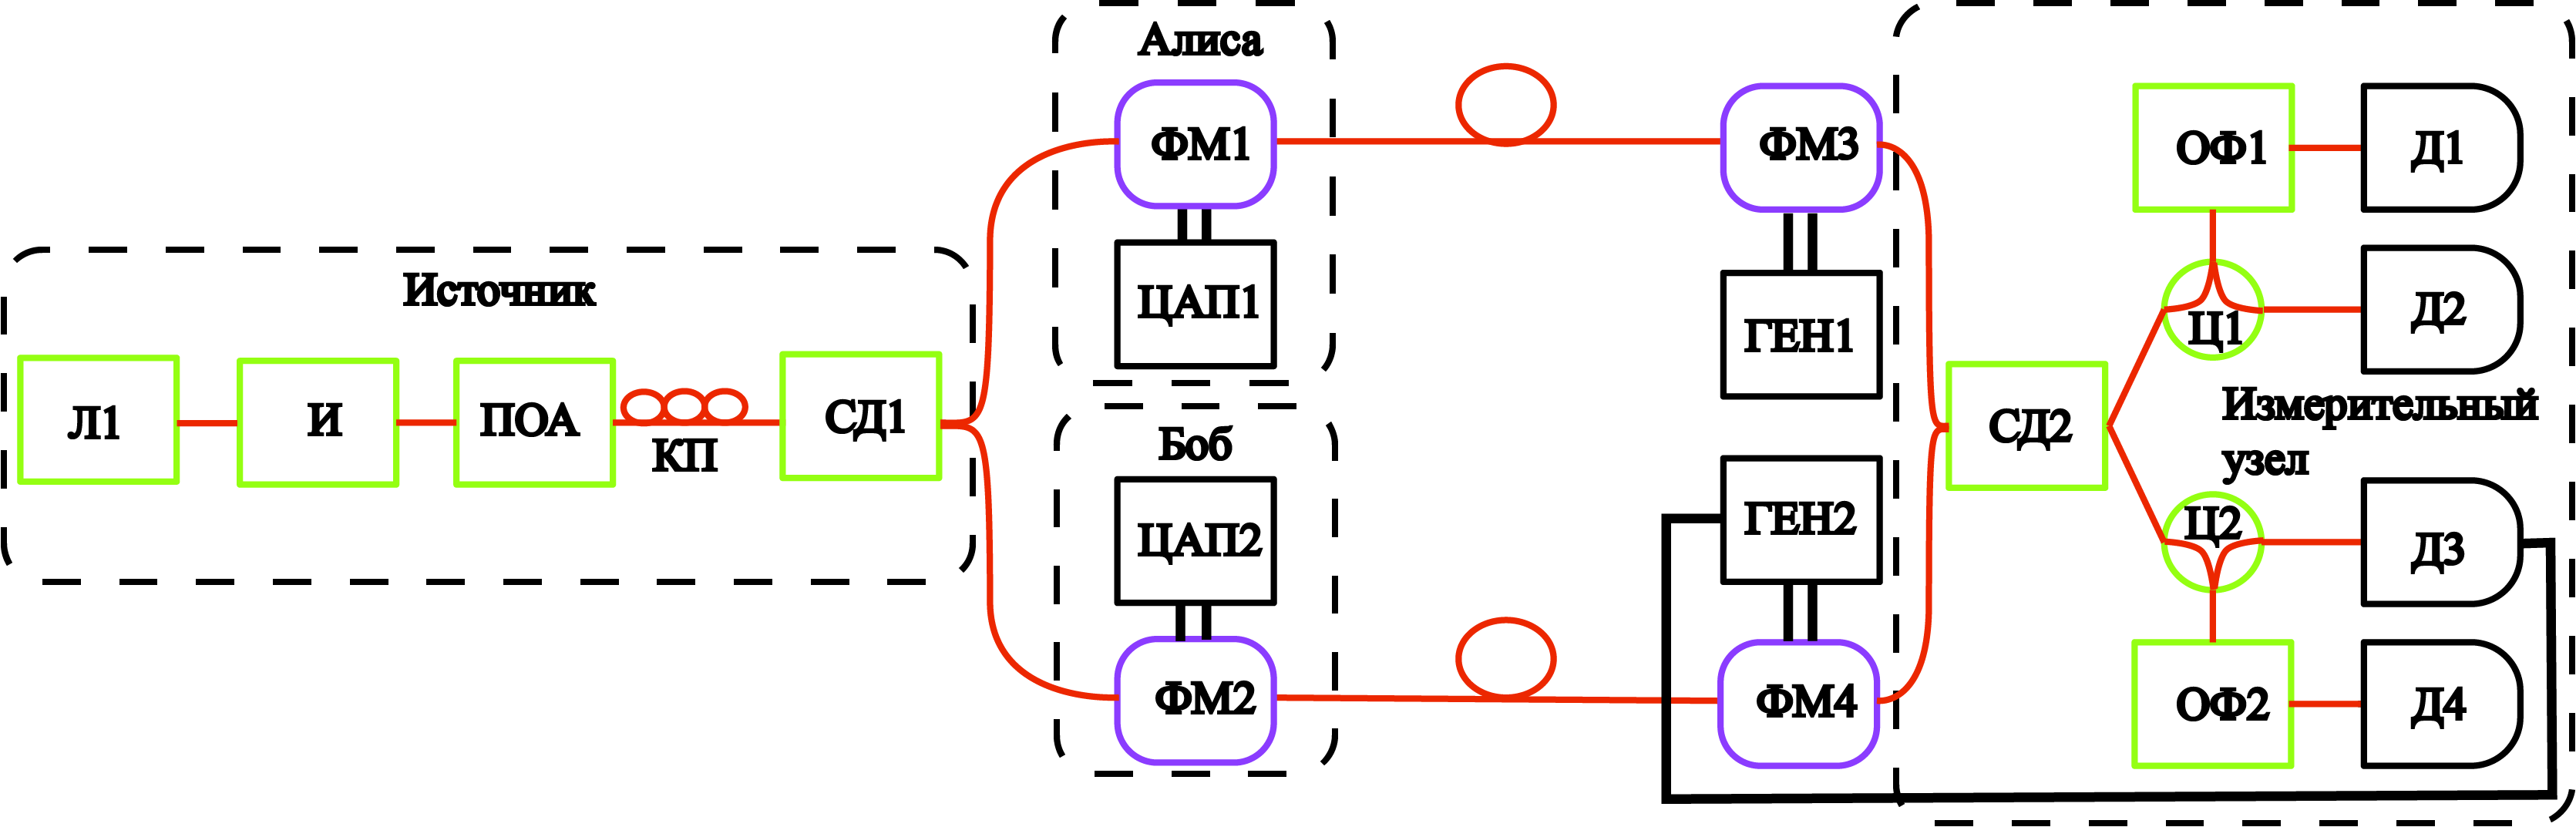
\includegraphics[scale=0.5]{Scheme_colored_rus.png}
  \caption{Принципиальная схема экспериментального стенда}
  \label{fig:RF_sin}
\end{figure}

На выходе из источника сигнал проходил по двум плечам формируемого таким образом интерферометра через светоделитель, благодаря чему имитировалось, что Алиса и Боб - это раздельные узлы, в которых информация кодировалась с помощью фазовых модуляторов. Выходы первого светоделителя подключались ко входам двух независимых 10~ГГц электро-оптических модуляторов на основе $LiNbO_3$ (со встроенным поляризатором) $ФМ1$ and $ФМ2$. Поляризаторы снижали чувствительность модуляторов к поляризации входного излучения, для чего использовался контроллер поляризации КП, и таким образом, повышалась видность картины интерференции. Электрические входы $ФМ1$ и $ФМ1$ подключались к выходам с цифро-аналоговых преобразователей ЦАП с модулирующим радиочастотным синусоидальным сигналом (с частотой 4,8~ГГц). Амплитуды управляющих сигналов подбирались таким образом, чтобы мощность сигнала на боковых частотах была равно у Алисы и у Боба. 

% and provide 0.2 photons intensity of sidebands.

Индекс модуляции, который показывает долю энергии на боковых частотах по отношению к центральной в результате модуляции должен быть 5~\%. В таком случае наблюдается оптимальное соотношение сигнала на боковых частотах к шуму проходящей через оптический фильтр центральной частоты.  Так что средняя величина оптической мощности была равна 2.56~пВт, что соответствует $\mu=0.2$.  


В данном исследовании  использовались только два кодирующих фазовых состояния на Алисе и Бобе ($\varphi_{A,B}\in\{0,\pi\}$. Разница фаз ($\Delta\varphi$) между Алисой и Бобом формировалась с помощью изменения IQ-таблиц ЦАП при помощь ПЛИС и ПО сосбтвенной разработки. В случае измерения зависимости количества срабатываний детекторов от разности фаз ($\Delta\varphi$) фаза сдвигалась последовательно с шагом $\varphi_{step}\ = 10^{\circ}$. Наблюдаемые состояния на выходах $ФМ1$ и $ФМ2$ могут быть описаны в соотвествии с уравнением~\ref{phi}.

После того, как состояния приготовлены, мы посылаем их в квантовый канал. Для компенсации оптической разности хода в двух плечах интерферометра, а так же для точной подстройки оптических фаз сигналов использовались $ФМ3$ и $ФМ4$. Эта подстройка осуществлялась при помощи изменения постоянного напряжения, подаваемого на модуляторы и формируемого двумя независимыми электрическими выходами генератора сигналов $GEN1$ и $GEN2$. Выходы втрой пары фазовых модуляторов подключались к паре входных портов светоделителя $СД2$ 2x2 с коэффициентом деления 50:50.

Измерения проводились в два этапа: первый этап в классическом свете, второй этап - в режиме счета фотонов на сверхпроводниковом детекторе одиночных фотонов (Сконтел), у которого встроены два независимых приёмника $Д1$, $Д4$. Квантовая эффективность обоих была равна 10~\%, а уровень темновых шумов не превышал 50~Гц для каждого. Измеренная величина суммарных шумов, включающих в себя темновые срабатывания и засветку от центральной частоты в силу ограниченной экстинкции оптического фильтра, составляла $\gamma_{темн}=1.5$ кГц.

Фотография экспериментального стенда представлена на рисунке \ref{fig:experimental_setup_TF}.  

 \begin{figure}[ht]
  \centering
	 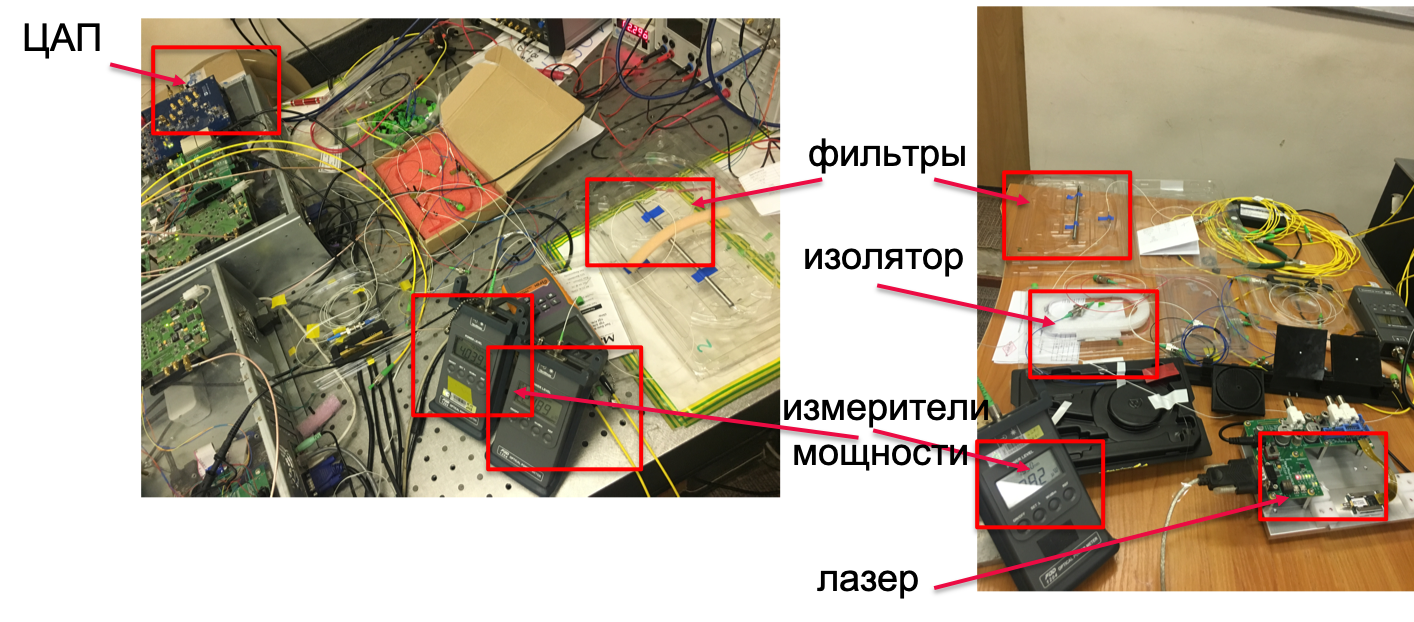
\includegraphics[scale=0.7]{Experimental_setup_TF}
  \caption{Фотография экспериментального стенда}
  \label{fig:experimental_setup_TF}
\end{figure}

\pagebreak

%%%%%%%%%%%%%%%%%%%%%%%%%%%%%%%%%%%%%%%%%%%%%%%%%%%%%%%%%%%%%%%%%%%%%%%%%%%%%%%%%
\section{Характеристики компонентов экспериментального стенда} \label{ch:ch5/sec2}

Значительную трудность представляет согласование спектральных характеристик Алисы и Боба. Даже при использовании одного источника для имитации хорошо скоррелированных лазеров, требуется подобрать оптические фильтры с максимально совпадающими характеристиками. В системе квантовой коммуникации частота модулирующего сигнала равна $\Omega = 4,8$~ГГц (рис.\ref{fig:RF_sin_osc} ). Значит, полоса спектрального фильтра не должна превышать величину $2\Omega$. Для этих целей используются волоконные узкополосные оптические фильтры на основе Брэгговских решеток. На рисунке \ref{fig:Spectrums} показаны измеренные характеристики максимально близких по серединному значению полосы пропускания фильтров. Уровень полуширины (FWHM) первого фильтра ОФ1 равен 48,8~пм (или 6,1~ГГц), а уровень полуширины (FWHM) второго фильтра ОФ2 равен 40~пм (или 5~ГГц). При этом разность центральных длин волн составляет 8~пм (или 1~ГГц). В ходе эксперимента лазер подстраивался таким образом, чтобы минимальная величина засветки от центральной проходила через оба оптических фильтра. Из-за несовпадения их характеристик повышался уровень шумов, вследствие чего ухудшалась видность картины интерференции.  

 \begin{figure}[ht]
  \centering
  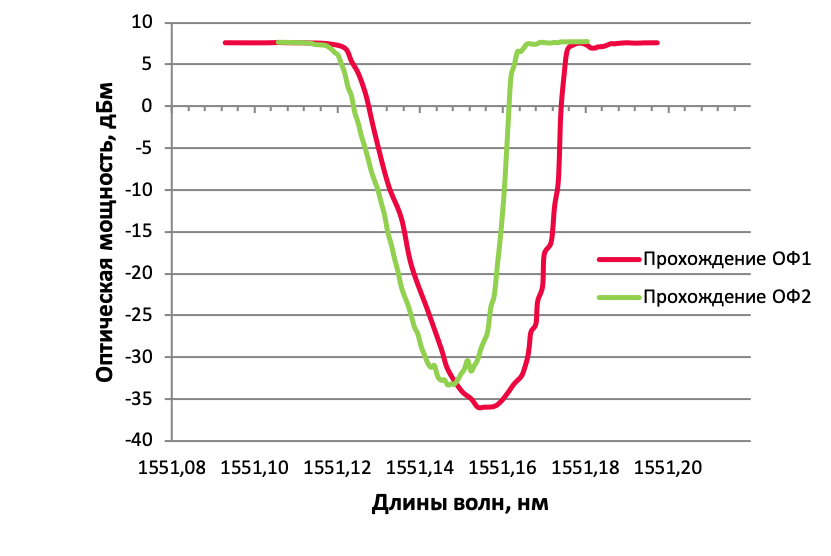
\includegraphics[scale=0.8]{T-spectrums.png}
  \caption{Спектральные характеристики оптических фильтров}
  \label{fig:Spectrums}
\end{figure}

\pagebreak

%%%%%%%%%%%%%%%%%%%%%%%%%%%%%%%%%%%%%%%%%%%%%%%%%%%%%%%%%%%%%%%%%%%%%%%%%%%%%%%%%%%%%%%%%%%%%%%%%%%%%%%%%%%%%%%%%
%\section{Экспериментальный стенд} \label{ch:ch5/sec3}


%\pagebreak

%%%%%%%%%%%%%%%%%%%%%%%%%%%%%%%%%%%%%%%%%%%%%%%%%%%%%%%%%%%%%%%%%%%%%%%%%%%%%%%%%%%%%%%%%%%%%%%%%%%%%%%%%%%%%%%%%
\section{Зависимость интенсивности на боковых частотах от сдвига фаз в результате интерференции в классическом режиме} \label{ch:ch5/sec5}

 \begin{figure}[ht]
  \centering
  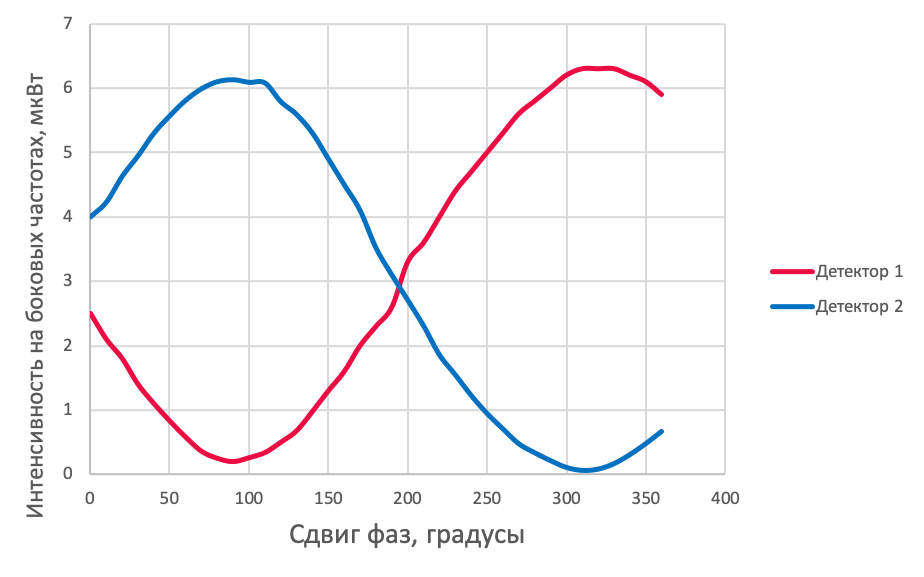
\includegraphics[scale=0.7]{Experimental_TF_classical.png}
  \caption{Зависимость интенсивности на боковых частотах в результате интерференции от разности фаз модулирующих сигналов}
  \label{fig:Experimental_TF_classical}
\end{figure}

\pagebreak

%%%%%%%%%%%%%%%%%%%%%%%%%%%%%%%%%%%%%%%%%%%%%%%%%%%%%%%%%%%%%%%%%%%%%%%%%%%%%%%%%%




\section{Вероятности срабатываний детекторов} \label{ch:ch5/sec6}

 Известно, что оптический фильтр отражает центральную оптическую моду ($k=0$). Значит, среднее число фотоном на входе в каждый детектор может быть найдена как \ref{nph1}. 
 
\begin{align}\label{nph1}
    n(\Delta\varphi)_{1,2}&=\mu_0\eta_c\Bigg(\sum_{k\neq 0}|d_{0k}^{S}(\beta)|^2 + \vartheta|d_{0k}^{S}(\beta)|^2 \pm \nonumber \\
    &\pm \cos(\varphi_0)\Big(\sum_{k\neq 0}|d_{0k}^{S}(\beta)|^2e^{i\Delta\varphi k}+ \vartheta|d_{0k}^{S}(\beta)|^2 \Big) \Bigg),
\end{align}

где $\Delta\varphi=\varphi_B-\varphi_A$, $\varphi_0$ это относительная оптическая фаза между импульсами отправителя (Алисы) и получателя (Боб), $\vartheta \ll 1$ часть центральной моды ($k=0$) проходящая через фильтр, ввиду ограниченности его характеристики. Используя свойства d-функци из \cite{varshalovich1988quantum}, можно упростить предыдущее выражение \ref{nph}

\begin{align}
    n(\Delta\varphi)_{1,2}=\mu_0\eta_c\Big(1-(1-\vartheta)(1\mp\cos(\varphi_0))|d_{00}^{S}(\beta)|^2 \pm \nonumber \\
    \pm\cos(\varphi_0)d_{00}^{S}(\beta')\Big) \label{nph},
\end{align}

где аргумент $\beta'$ получен следующим образом \ref{betaappox}. 

\begin{equation} \label{betaappox}
    \cos(\beta')=\cos^2(\beta) \mp \sin^2(\beta)\cos(\Delta\varphi).
\end{equation}

Чтобы оценить вероятность срабатывания воспользуемся линейным приближением Манделя, предполагая слабые интенсивности ($n(\Delta\varphi)_{1,2} \ll 1$):

\begin{eqnarray}
    \mathcal{P}_{1,2}^{+}(\Delta\varphi)=\left(n(\Delta\varphi)_{1,2}\eta_DF+\gamma_{dark}\right)\Delta t, \label{pdet}
\end{eqnarray}

где $\eta_D$ квантовая эффективность, $F$ частота смены состояний, $\gamma_{dark}$ частота темновых отсчетов детектора одиночных фотонов, и $\Delta t$ время окна срабатывания. Для простоты положим $\Delta t F=1$. Отсутствие срабатывания определим, как $\mathcal{P}_{1,2}^{-}(\Delta\varphi)=1-\mathcal{P}_{1,2}^{+}(\Delta\varphi)$.     


Используем несколько полезных приближений, которые помогут оценить квантовый коэффициент ошибок по битам (QBER) и скорости формирования просеянного ключа. Для начала положим, что число взаимодействующих мод велико ($S\rightarrow \infty$), что действительно так для стандартных волоконно-оптических модуляторов. Тогда можно использовать приближение d-функций следующим образом:

\begin{align}
d_{nk}^S(\beta) &\xrightarrow{S\rightarrow \infty} J_{n-k}(m), \label{limdj} \\
\beta &\propto m, \label{propto}
\end{align}
где $J_k(m)$ функция Бесселя первого порядка. Полагая значение $m$ малым, что действительно так, в соотвествии с теорией классической модуляции воспользуемся приближением первого порядка функции Бесселя. 


Так в соответствии с уравнение \ref{betam} $\beta \rightarrow 0$, следовательно можно использовать аппроксимации первого порядка для выражения \ref{betaappox} в терминах $m$ подразумевая пропорциональность в уравнении \ref{propto}.


Определим уравнение~\ref{pdet} следующим образом:

\begin{align}\label{pdet1}
 \mathcal{P}_{1,2}^{+}(\Delta\varphi)&=\mu\eta\Big(1\pm\cos(\Delta\varphi)\cos(\varphi_0)\Big)+ \nonumber
 \\
 &+\vartheta\Big(\mu_c\eta(1\pm\cos(\varphi_0))\Big)+p_{dark},
\end{align}


где $\eta$ полная оптическая пропускная способность квантового канала с учетом квантовой эффективности детектора, $p_{dark}=\gamma_{dark}\Delta t$ это вероятность темнового срабатывания во временном интервале $\Delta t$, и $\mu$ и $\mu_c$ это среднее число фотонов на боковых и на центральной моде соотвественно после модуляции, как определено:

\begin{align}
    \mu&=\mu_0\sum_{k\neq 0}|d_{0k}^{S}(\beta)|^2, \\
    \mu_c&=\mu_0-\mu=\mu_0(1-\sum_{k\neq 0}|d_{0k}^{S}(\beta)|^2).
\end{align}
Выраение в уравнени~\ref{pdet1} даёт точное соотношение между экспериментальными параметрами и показывает, как они влияют на вероятности детектирования квантовых состояний. 


\pagebreak

%%%%%%%%%%%%%%%%%%%%%%%%%%%%%%%%%%%%%%%%%%%%%%%%%%%%%%%%%%%%%%%%%%%%%%%%%%%%%%%%%%
\section{Зависимость интенсивности на боковых частотах от сдвига фаз в результате интерференции в режиме счета фотонов} \label{ch:ch5/sec7}


 \begin{figure}[ht]
  \centering
  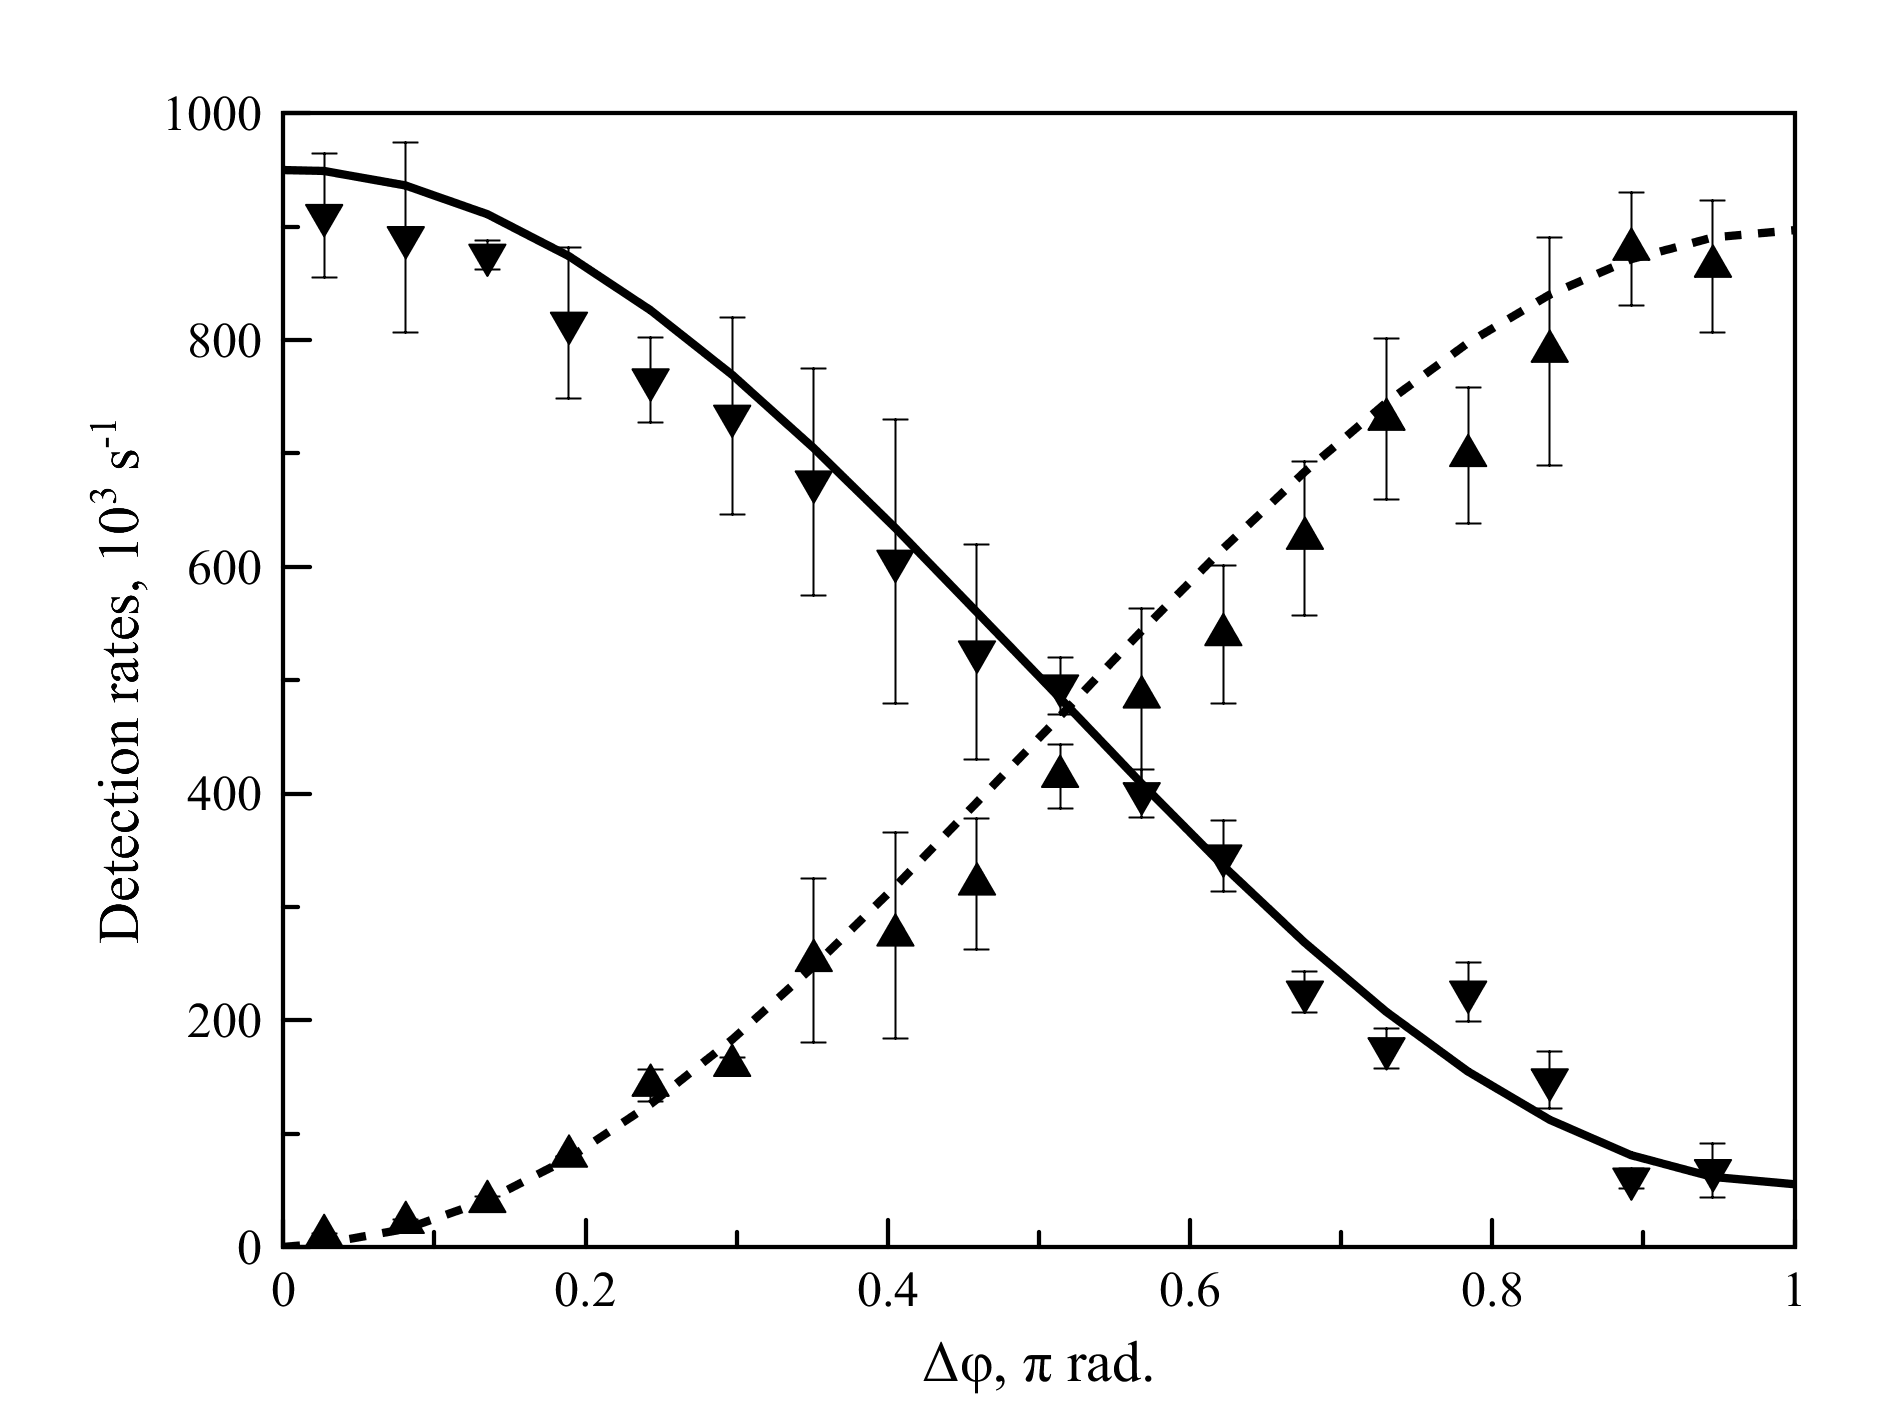
\includegraphics[scale=0.2]{ExperimentTF.png}
  \caption{Зависимость количества отсчетов в результате интерференции от разности фаз модулирующих сигналов}
  \label{fig:Experimental_TF}
\end{figure}


\pagebreak

%%%%%%%%%%%%%%%%%%%%%%%%%%%%%%%%%%%%%%%%%%%%%%%%%%%%%%%%%%%%%%%%%%%%%%%%%%%%%%%%%%
\section{Оценка коэффициента битовых ошибок и скорости формирования ключа} \label{ch:ch5/sect8}

Далее рассмотрим только те случаи, где срабатывание происходит только на одном из детекторов в единицу времени.  Таким образом, вероятности срабатываний $R$ определяются как:

\begin{align}
    R&=\Big(\mathcal{P}_{1}^{+}\mathcal{P}_{2}^{-}(\Delta\varphi=\varphi_m)+\mathcal{P}_{1}^{-}\mathcal{P}_{2}^{+}(\Delta\varphi=\pi+\varphi_m)+ \nonumber \\
    &+\mathcal{P}_{1}^{+}\mathcal{P}_{2}^{-}(\Delta\varphi=\pi+\varphi_m)+\mathcal{P}_{1}^{-}\mathcal{P}_{2}^{+}(\Delta\varphi=\varphi_m)\Big),
\end{align}


где $\varphi_m$ средняя величина несоответствия фаз $\varphi_A$ и $\varphi_B$. Первые два слагаемых - это вероятности успешного определения битов легитимными пользователями, тогда как оставшиеся два слагаемых - вероятности смены бита на противоположный (bitflip) (полагая $\varphi_0 \approx 0$). Таким образом, можно определить выражение для QBER $Q$ следующим образом:

\begin{align}
    Q=\frac{\mathcal{P}_{1}^{-}\mathcal{P}_{2}^{+}(\Delta\varphi=\varphi_m)+\mathcal{P}_{1}^{+}\mathcal{P}_{2}^{-}(\Delta\varphi=\pi+\varphi_m)}{R}.
\end{align}


Наконец, можно определить выражение для оценки среднего значения скорости формирования просеянного ключа $K$ (одинаковые биты между легитимными пользователями, но коррелирующие с возможным результатом у злоумышленника, что требуется проведения процедуры усиления секретности)
\begin{equation}
    K=FR(1-h(Q)),
\end{equation}
где $h(Q)$ это функция двоичной энтропии. 

\pagebreak

%%%%%%%%%%%%%%%%%%%%%%%%%%%%%%%%%%%%%%%%%%%%%%%%%%%%%%%%%%%%%%%%%%%%%%%%%%%%%%%%%%
\section{Выводы по главе} \label{ch:ch5/sec9}


В \ref{ch:ch5} главе показано, что в результате интерференции квантового фазомодулированного сигнала на боковых частотах на симметричном светоделителе в схеме квантовой рассылки ключа с узлом регистрации, независящим от легитимного пользователя, происходит спектральное разделение квантового сигнала и сигнала на центральной длине волны с их независимой регистрацией в разных плечах светоделителя. 

\pagebreak
           % Глава 5
\chapter{Анализ секретности системы квантовой коммуникации с недоверенным приемным узлом} \label{ch:ch6}
\section{Исследование возможностей злоумышленника по получению информации о квантовом состоянии при разделении многофотонных состояний} \label{sec:ch6/sec1}

Пусть $|\alpha e^{i \varphi}\rangle$ - слабое когерентное состояниие, где $\alpha$ - это амплитуда состояния, а $\varphi$ - фаза, с помощью которой кодируется бит. Вероятность наблюдения ожидаемого результата измерения, говорящего о наличии $n$ фотонов в данном примере или импульсе, может быть получена с учетом следа продукта матрицы плотности когерентного состояния $\rho$ и проектора на Фоковский базис $|n\rangle\langle n|$: 
%
\begin{align}
    P_n&=\text{Tr}(\rho |n\rangle\langle n|) = \text{Tr}(|\alpha e^{i \varphi}\rangle \langle\alpha e^{i \varphi} |n\rangle\langle n|) \nonumber \\
    &= \text{Tr}(\sum_{k=0}^{\infty}\sum_{m=0}^{\infty} e^{-|\alpha|^2} \frac{(\alpha e^{i \varphi})^k(\alpha^{*} e^{-i \varphi})^m}{\sqrt{k!m!}} |k\rangle\langle m |n\rangle\langle n|) \nonumber  \\
    &=\sum_{j=0}^{\infty}\sum_{k=0}^{\infty}\sum_{m=0}^{\infty} e^{-|\alpha|^2} \frac{(\alpha e^{i \varphi})^k(\alpha^{*} e^{-i \varphi})^m}{\sqrt{k!m!}}\langle j |k\rangle\langle m |n\rangle\langle n|j\rangle \nonumber  \\
    &=e^{-|\alpha|^2} \frac{(|\alpha|^{2n})}{n!}, \label{pnver}
\end{align}
% 
где мы используем свойство ортогональности векторов Фоковского базиса $\langle k| n \rangle = \delta_{kn}$, где $\delta_{kn}$ - дельта-символ Кронекера. Таким образом, мы можем представить слабое когерентное состояние в Фоковском базисе, как:
%
\begin{equation}
    |\alpha e^{i \varphi}\rangle = e^{-\frac{|\alpha|^2}{2}}\sum_{n=0}^{\infty}  \frac{(\alpha e^{i \varphi})^n}{\sqrt{n!}} |n\rangle.
\end{equation}
%
Следовательно, состояние после измерения может быть сокращено следующим образом:
%
\begin{equation}
    \Tilde{\rho}=\frac{\sqrt{|n\rangle\langle n|} |\alpha e^{i \varphi}\rangle \langle\alpha e^{i \varphi} | \sqrt{|n\rangle\langle n|}}{P_n}.
\end{equation}
%
Исследуем, как оператор $\sqrt{|n\rangle\langle n|}$ воздействует на вектор в Фоковском базисе $|m\rangle$, представляя его в виде ряда Тейлора. Рассмотрим два различных случая:
%
\begin{enumerate}
    \item $m \neq n$
    \begin{align}
        \sqrt{|n\rangle\langle n|}|m\rangle = \sum_{k=0}^{\infty} \frac{(-1)^k(2k)!}{(1-2k)(k!)^2 4^k}(|n\rangle\langle n|-\hat{I})^k|m\rangle ,
    \end{align}
    где $\hat{I}$ оператор тождества. Используя следующие свойства
    \begin{gather}
        \hat{I}|m\rangle=|m\rangle, \\
        (|n\rangle\langle n|)^k |m\rangle = (|n\rangle\langle n|)^{k-1} |n\rangle\langle n|m\rangle = 0,
    \end{gather}
    получаем
    \begin{align}
       \sqrt{|n\rangle\langle n|}|m\rangle = \sum_{k=0}^{\infty} \frac{(-1)^k(2k)!}{(1-2k)(k!)^2 4^k}(-1)^k|m\rangle = 0 |m\rangle.
    \end{align}
    \item $m=n$
    
   Затем, используя следующие свойства
    \begin{align}
        (|n\rangle\langle n|)^k |n\rangle = (|n\rangle\langle n|)^{k-1}=\nonumber\\ =|n\rangle\langle n|n\rangle = (|n\rangle\langle n|)^{k-1} |n\rangle = ... = |n\rangle,
    \end{align}
    тогда
    \begin{align}
        \sqrt{|n\rangle\langle n|}|n\rangle &= \sum_{k=0}^{\infty} \frac{(-1)^k(2k)!}{(1-2k)(k!)^2 4^k}(|n\rangle\langle n|-\hat{I})^k|n\rangle \nonumber\\
        &=|n\rangle + \sum_{k=1}^{\infty} \frac{(-1)^k(2k)!}{(1-2k)(k!)^2 4^k}(|n\rangle\langle n|-\hat{I})^k|n\rangle \nonumber\\
        &=|n\rangle + 0 = |n\rangle.
    \end{align}
\end{enumerate}
%
Таким образом, в сокращенном виде:
%
\begin{align}
   \Tilde{\rho}&=\frac{1}{P_n}\sum_{k=0}^{\infty}\sum_{m=0}^{\infty} e^{-|\alpha|^2} \frac{(\alpha e^{i \varphi})^k(\alpha^{*} e^{-i \varphi})^m}{\sqrt{k!m!}} \sqrt{|n\rangle\langle n|}|k\rangle\langle m |\sqrt{|n\rangle\langle n|} \nonumber \\
   &= \frac{1}{P_n} P_n |n\rangle\langle n| = |n\rangle\langle n|. \label{rhored}
\end{align}
%
Тем самым, в соответствии с выражениями, полученными в~\ref{pnver} и \ref{rhored} результат измерения числа фотонов в импульсе (проекция на Фоковский базис) в слабом когерентном импульсе и сокращенное состояние после измерения не содержат информации о фазе когерентного состояния $\varphi$. В случае с множеством мод, проблема сводится к случаю с одной модой, описанному выше.
\pagebreak

%%%%%%%%%%%%%%%%%%%%%%%%%%%%%%%%%%%%%%%%%%%%%%%%%%%%%%%%%%%%%%%%%%%%%%%%%%%%%%%%%
\section{Оценка скорости формирования секретного ключа в асимптотическом приближении} \label{ch:ch6/sec2}

Finally one may derive expression that estimates average sifted key rates $C$ (identical bits but correlated with Eve hence privacy amplification is necessary)
\begin{equation}
    C=FR(1-h(Q)),
\end{equation}
where $h(Q)$ is binary entropy function.

To provide asymptotic key rates we use well-known method introduced by Devetak-Winter \cite{devetak2005distillation}.

We have estimated Holevo information for multi-mode coherent states presented in Eq.~\ref{phi} according to \cite{kozubov2019finite}:
\begin{equation}
    \chi=h\left(\frac{1-e^{-\mu_0(1-d^S_{00}(2\beta))}}{2}\right)\approx h\left(\frac{1-e^{-2\mu}}{2}\right).
\end{equation}
It shows us the maximal amount of information Eve may obtain from the states in one channel. However TF QKD schemes have two independent channels. Hence Eve can perform independent measurements in two quantum channels and obtain the following amount of information:
\begin{equation}
    \tilde{\chi}=2(1-\chi)\chi+\chi^2.
\end{equation}
Thus asymptotic secure key rates $K$ is as follows:
\begin{equation}
     K=FR(1-\xi h(Q)-\tilde{\chi}),
\end{equation}
where $\xi$ is the error correction efficiency. 
For calculations we use experimental parameters from one of the regimes used in Ref.~\cite{Gleim16,Miroshnichenko18}, which are close the implemented during experimental verification of our model: $F=100$ MHz, $\mu=0.1$, $\mu_0=4$, $\Delta\varphi=5^{\circ}$, $\vartheta=10^{-3}$, $\xi=1.15$, $\varphi_0=5^{\circ}$ $\eta_D=0.25$, $\gamma_{dark}= 10$ Hz. The simulation results are shown in Fig.~\ref{fig:fig2}.

\begin{figure}
	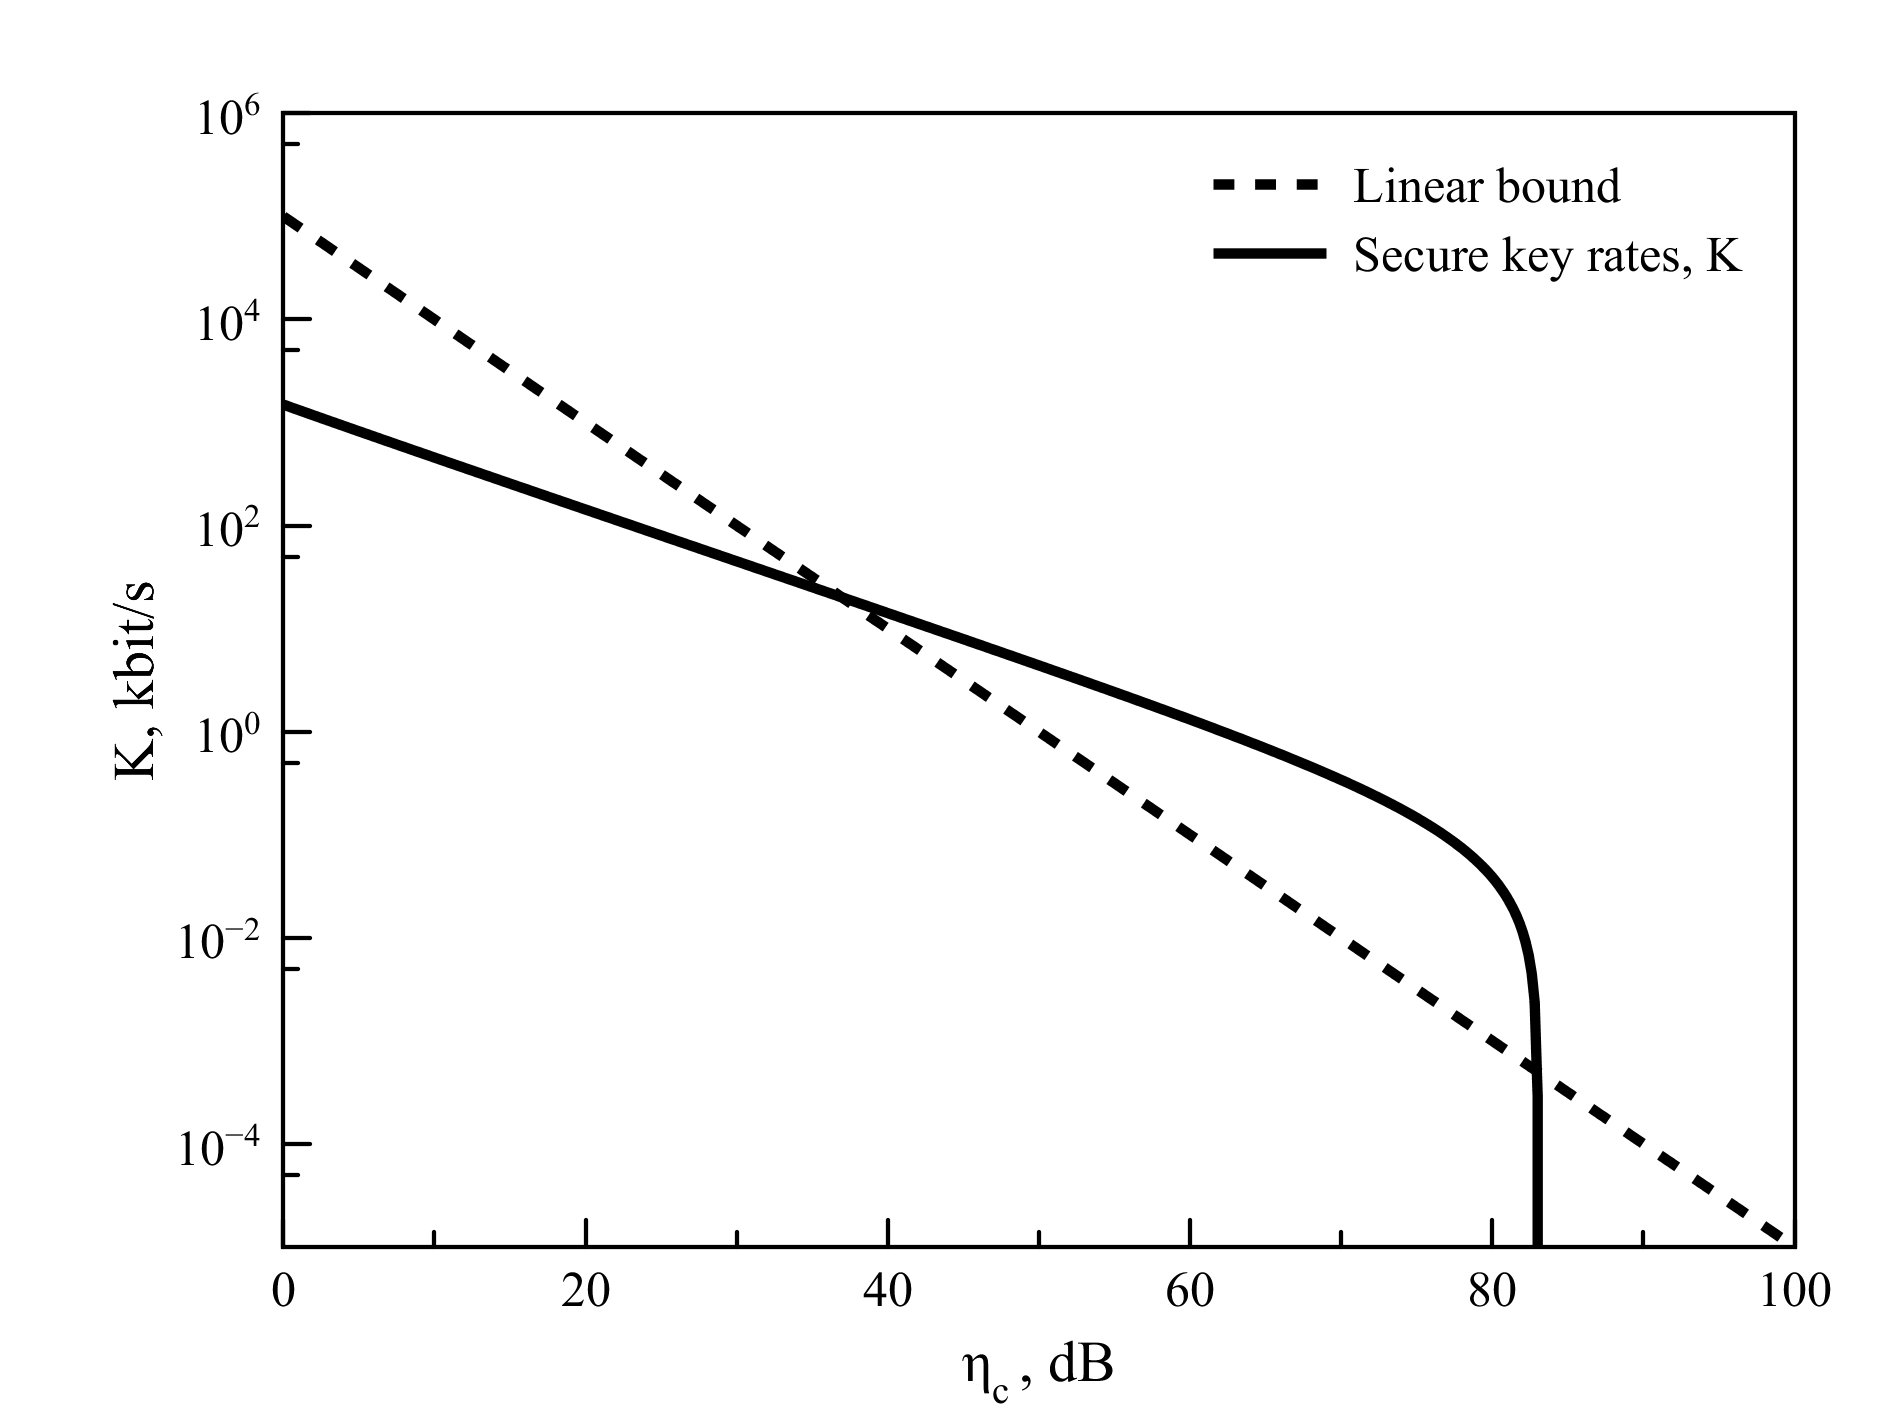
\includegraphics[width=1\linewidth]{TFQKD.png}
	\caption{ Simulation of our TF QKD protocol based on multi-mode phase-coded weak coherent states. For the considered simulation parameters, the key rate of proposed TF QKD exceeds the linear key rate bound by Pirandola et al. (PLOB bound) \cite{pirandola2017fundamental} when $\eta_c \gtrsim$ 40 dB (200 km). In addition, our protocol is also able to achieve a long transmission distance of $\eta_c\approx$ 83 dB (460 km). %Parameters were estimated as follows: $\mu=0.2$, $\mu_0=4$, $F=100$ MHz, $\gamma_{dark}=1.5$ kHz, $\vartheta=10^{-2.5}$, $\varphi_0\approx0$, $\eta=10^{-1.65}$, $\varphi_m\approx3^{\circ}$.} 
	}
	\label{fig:fig2}
\end{figure}


Наконец, можно определить выражение для оценки среднего значения скорости формирования просеянного ключа $K$ (одинаковые биты между легитимными пользователями, но коррелирующие с возможным результатом у злоумышленника, что требует проведения процедуры усиления секретности)
\begin{equation}
    K=FR(1-h(Q)),
\end{equation}
где $h(Q)$ это функция двоичной энтропии. 

\pagebreak

%%%%%%%%%%%%%%%%%%%%%%%%%%%%%%%%%%%%%%%%%%%%%%%%%%%%%%%%%%%%%%%%%%%%%%%%%%%%%%%%%%
\section{Выводы по главе} \label{ch:ch6/sec9}


В \ref{ch:ch6/sec2}  

\pagebreak

           % Глава 6 Штатная 1
\chapter{Длинное название главы, в которой мы смотрим на~примеры того, как будут верстаться изображения и~списки} \label{ch:ch7}

\section{Одиночное изображение} \label{sec:ch7/sec1}

\begin{figure}[ht]
  \centering
  
\includegraphics [scale=0.27] {latex}
  \caption{TeX.}
  \label{fig:latex}
\end{figure}

\section{Длинное название параграфа, в котором мы узнаём как сделать две картинки с~общим номером и названием} \label{sec:ch7/sect2}

А это две картинки под общим номером и названием:
\begin{figure}[ht]
  \begin{minipage}[ht]{0.49\linewidth}\centering
    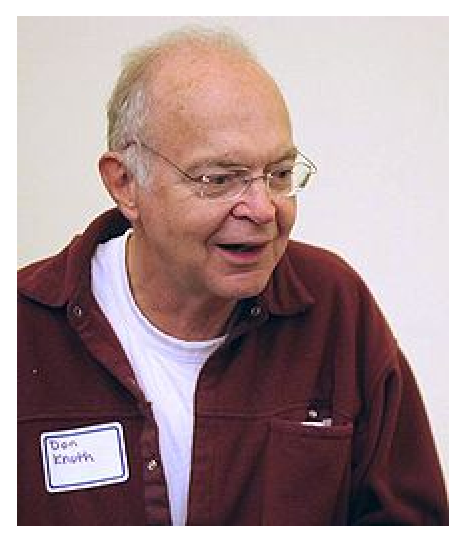
\includegraphics[width=0.5\linewidth]{knuth1} \\ а)
  \end{minipage}
  \hfill
  \begin{minipage}[ht]{0.49\linewidth}\centering
    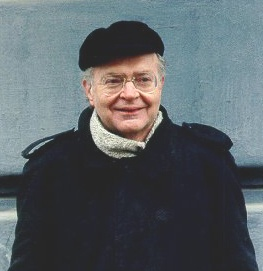
\includegraphics[width=0.5\linewidth]{knuth2} \\ б)
  \end{minipage}
  \caption{Очень длинная подпись к изображению,
      на котором представлены две фотографии Дональда Кнута}
  \label{fig:knuth}
\end{figure}

Те~же~две картинки под~общим номером и~названием,
но с автоматизированной нумерацией подрисунков:
\begin{figure}[ht]
    {\centering
        \hfill
        \subbottom[List-of-Figures entry][Первый подрисунок\label{fig:knuth_2-1}]{%
            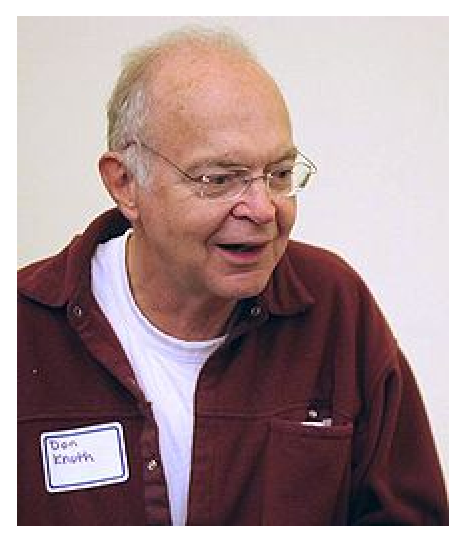
\includegraphics[width=0.25\linewidth]{knuth1}}
        \hfill
        \subbottom[\label{fig:knuth_2-2}]{%
            \includegraphics[width=0.25\linewidth]{knuth2}}
        \hfill
        \subbottom[Третий подрисунок]{%
            \includegraphics[width=0.3\linewidth]{example-image-c}}
        \hfill
    }
    \legend{Подрисуночный текст, описывающий обозначения, например. Согласно
    ГОСТ 2.105, пункт 4.3.1, располагается перед наименованием рисунка.}
    \caption[Этот текст попадает в названия рисунков в списке рисунков]{Очень
    длинная подпись к второму изображению, на~котором представлены две
    фотографии Дональда Кнута}
    \label{fig:knuth_2}
\end{figure}

На рисунке~\ref{fig:knuth_2-1} показан Дональд Кнут без головного убора.
На рисунке~\ref{fig:knuth_2}\subcaptionref*{fig:knuth_2-2}
показан Дональд Кнут в головном уборе.

Возможно вставлять векторные картинки, рассчитываемые \LaTeX\ <<на~лету>>
с~их~предварительной компиляцией. Надписи в таких рисунках будут выполнены
тем же~шрифтом, который указан для документа в целом.
На~рисунке~\ref{fig:tikz_example} на~странице~\pageref{fig:tikz_example}
представлен пример схемы, рассчитываемой пакетом \verb|tikz| <<на~лету>>.
Для ускорения компиляции, подобные рисунки могут быть <<кешированы>>, что
определяется настройками в~\verb|common/setup.tex|.
Причём имя предкомпилированного
файла и~папка расположения таких файлов могут быть отдельно заданы,
что удобно, если не~для подготовки диссертации,
то~для подготовки научных публикаций.
\begin{figure}[ht]
    {\centering
        \ifdefmacro{\tikzsetnextfilename}{\tikzsetnextfilename{tikz_example_compiled}}{}% присваиваемое предкомпилированному pdf имя файла
        % !TEX encoding = UTF-8 Unicode
% Úτƒ-8 encoded
% http://www.linux.org.ru/forum/general/10357036
\tikzset{
    line/.style={draw, -latex'},
    every join/.style={line},
    u/.style={anchor=south},
    r/.style={anchor=west},
    fxd/.style={text width = 6em},
    it/.style={font={\small\itshape}},
    bf/.style={font={\small\bfseries}}
}
\tikzstyle{base} =
    [
        draw,
        on chain,
        on grid,
        align=center,
        minimum height=4ex,
        minimum width = 10ex,
        node distance = 6mm and 60mm,
        text badly centered
    ]
\tikzstyle{coord} =
    [
        coordinate,
        on chain,
        on grid
    ]
\tikzstyle{cloud} =
    [
        base,
        ellipse,
        fill = red!5,
        node distance = 3cm,
        minimum height = 2em
    ]
\tikzstyle{decision} =
    [
        base,
        diamond,
        aspect=2,
        fill = green!10,
        node distance = 2cm,
        inner sep = 0pt
    ]
\tikzstyle{block} =
    [
        rectangle,
        base,
        fill = blue!3,
        rounded corners,
        minimum height = 2em
    ]
\tikzstyle{print_block} =
    [
        base,
        tape,
        tape bend top=none,
        fill = yellow!10
    ]
\tikzstyle{io} =
    [
        base,
        trapezium,
        trapezium left angle = 70,
        trapezium right angle = 110,
        fill = blue!5
    ]
\makeatletter
\pgfkeys{/pgf/.cd,
    subrtshape w/.initial=2mm,
    cycleshape w/.initial=2mm
}
\pgfdeclareshape{subrtshape}{
    \inheritsavedanchors[from=rectangle]
    \inheritanchorborder[from=rectangle]
    \inheritanchor[from=rectangle]{north}
    \inheritanchor[from=rectangle]{center}
    \inheritanchor[from=rectangle]{west}
    \inheritanchor[from=rectangle]{east}
    \inheritanchor[from=rectangle]{mid}
    \inheritanchor[from=rectangle]{base}
    \inheritanchor[from=rectangle]{south}
    \backgroundpath{
        \southwest \pgf@xa=\pgf@x \pgf@ya=\pgf@y
        \northeast \pgf@xb=\pgf@x \pgf@yb=\pgf@y
        \pgfmathsetlength\pgfutil@tempdima{\pgfkeysvalueof{/pgf/subrtshape w}}
        \def\ppd@offset{\pgfpoint{\pgfutil@tempdima}{0ex}}
        \def\ppd@offsetm{\pgfpoint{-\pgfutil@tempdima}{0ex}}
        \pgfpathmoveto{\pgfqpoint{\pgf@xa}{\pgf@ya}}
        \pgfpathlineto{\pgfqpoint{\pgf@xb}{\pgf@ya}}
        \pgfpathlineto{\pgfqpoint{\pgf@xb}{\pgf@yb}}
        \pgfpathlineto{\pgfqpoint{\pgf@xa}{\pgf@yb}}
        \pgfpathclose
        \pgfpathmoveto{\pgfpointadd{\pgfpoint{\pgf@xa}{\pgf@yb}}{\ppd@offsetm}}
        \pgfpathlineto{\pgfpointadd{\pgfpoint{\pgf@xa}{\pgf@ya}}{\ppd@offsetm}}
        \pgfpathlineto{\pgfpointadd{\pgfpoint{\pgf@xb}{\pgf@ya}}{\ppd@offset}}
        \pgfpathlineto{\pgfpointadd{\pgfpoint{\pgf@xb}{\pgf@yb}}{\ppd@offset}}
        \pgfpathclose
    }
}
\pgfdeclareshape{cyclebegshape}{
    \inheritsavedanchors[from=rectangle]
    \inheritanchorborder[from=rectangle]
    \inheritanchor[from=rectangle]{north}
    \inheritanchor[from=rectangle]{center}
    \inheritanchor[from=rectangle]{west}
    \inheritanchor[from=rectangle]{east}
    \inheritanchor[from=rectangle]{mid}
    \inheritanchor[from=rectangle]{base}
    \inheritanchor[from=rectangle]{south}
    \backgroundpath{
        \southwest \pgf@xa=\pgf@x \pgf@ya=\pgf@y
        \northeast \pgf@xb=\pgf@x \pgf@yb=\pgf@y
        \pgfmathsetlength\pgfutil@tempdima{\pgfkeysvalueof{/pgf/cycleshape w}}
        \pgfpathmoveto{\pgfqpoint{\pgf@xa}{\pgf@ya}}
\pgfpathlineto{\pgfpointadd{\pgfpoint{\pgf@xa}{\pgf@yb}}{\pgfpoint{0ex}{-\pgfutil@tempdima}}}
\pgfpathlineto{\pgfpointadd{\pgfpoint{\pgf@xa}{\pgf@yb}}{\pgfpoint{\pgfutil@tempdima}{0ex}}}
\pgfpathlineto{\pgfpointadd{\pgfpoint{\pgf@xb}{\pgf@yb}}{\pgfpoint{-\pgfutil@tempdima}{0ex}}}
\pgfpathlineto{\pgfpointadd{\pgfpoint{\pgf@xb}{\pgf@yb}}{\pgfpoint{0ex}{-\pgfutil@tempdima}}}
\pgfpathlineto{\pgfqpoint{\pgf@xb}{\pgf@ya}}
        \pgfpathclose
    }
}
\pgfdeclareshape{cycleendshape}{
    \inheritsavedanchors[from=rectangle]
    \inheritanchorborder[from=rectangle]
    \inheritanchor[from=rectangle]{north}
    \inheritanchor[from=rectangle]{center}
    \inheritanchor[from=rectangle]{west}
    \inheritanchor[from=rectangle]{east}
    \inheritanchor[from=rectangle]{mid}
    \inheritanchor[from=rectangle]{base}
    \inheritanchor[from=rectangle]{south}
    \backgroundpath{
        \southwest \pgf@xa=\pgf@x \pgf@ya=\pgf@y
        \northeast \pgf@xb=\pgf@x \pgf@yb=\pgf@y
        \pgfmathsetlength\pgfutil@tempdima{\pgfkeysvalueof{/pgf/cycleshape w}}
        \pgfpathmoveto{\pgfqpoint{\pgf@xb}{\pgf@yb}}
\pgfpathlineto{\pgfpointadd{\pgfpoint{\pgf@xb}{\pgf@ya}}{\pgfpoint{0ex}{\pgfutil@tempdima}}}
\pgfpathlineto{\pgfpointadd{\pgfpoint{\pgf@xb}{\pgf@ya}}{\pgfpoint{-\pgfutil@tempdima}{0ex}}}
\pgfpathlineto{\pgfpointadd{\pgfpoint{\pgf@xa}{\pgf@ya}}{\pgfpoint{\pgfutil@tempdima}{0ex}}}
\pgfpathlineto{\pgfpointadd{\pgfpoint{\pgf@xa}{\pgf@ya}}{\pgfpoint{0ex}{\pgfutil@tempdima}}}
\pgfpathlineto{\pgfqpoint{\pgf@xa}{\pgf@yb}}
        \pgfpathclose
    }
}
\makeatother
\tikzstyle{subroutine} =
    [
        base,
        subrtshape,
        fill = green!25
    ]
\tikzstyle{cyclebegin} =
    [
        base,
        cyclebegshape,
        fill = blue!25
    ]
\tikzstyle{cycleend} =
    [
        base,
        cycleendshape,
        fill = blue!25
    ]
\tikzstyle{connector} =
    [
        base,
        circle,
        fill = red!25
    ]

\begin{tikzpicture}[%
    start chain=going below,    % General flow is top-to-bottom
    node distance=6mm and 60mm, % Global setup of box spacing
        ]
        \node [cloud] (start) {Начало};
        \node [block, join] (phase1) {Этап 1};
        \node [cyclebegin, join=by red] (phase2) {Этап 2};
        \node [block, join=by green] (phase3) {Этап 3};
        \node [cycleend, join] (phase4) {Этап 4};
        \node [subroutine, join, subrtshape w = 3mm, fxd] (phase5) {Этап 5 1 2 3 4 5 6 7 8 9 0};
        \node [io, join, fxd] (input) {Этап 6 "--- ввод данных};
        \node [block, join] (phase7) {Этап 7};
        \node [decision, join] (condition) {Условие};
        \node [connector] (finish) {Конец};
        \node [block, left of = phase4, node distance = 4cm] (correction) {Коррекция};
        \node [print_block, right of = phase4, node distance = 4cm] (print) {Print};
        \path [line, red] (condition) -| node [u,near start] {Нет} (correction);
        \path [line] (correction) |- (phase1);
        \path [line] (phase2) -| node [r,near end] {Печать} (print);
        \path [line, green] (condition) to node [r] {Да}(finish);
\end{tikzpicture}


    }
    \legend{}
    \caption[Пример \texttt{tikz} схемы]{Пример рисунка, рассчитываемого
        \texttt{tikz}, который может быть предкомпилирован}
    \label{fig:tikz_example}
\end{figure}

Множество программ имеют либо встроенную возможность экспортировать векторную
графику кодом \verb|tikz|, либо соответствующий пакет расширения.
Например, в GeoGebra есть встроенный экспорт,
для Inkscape есть пакет svg2tikz,
для Python есть пакет matplotlib2tikz,
для R есть пакет tikzdevice.

\section{Пример вёрстки списков} \label{sec:ch7/sec3}

\noindent Нумерованный список:
\begin{enumerate}
  \item Первый пункт.
  \item Второй пункт.
  \item Третий пункт.
\end{enumerate}

\noindent Маркированный список:
\begin{itemize}
  \item Первый пункт.
  \item Второй пункт.
  \item Третий пункт.
\end{itemize}

\noindent Вложенные списки:
\begin{itemize}
  \item Имеется маркированный список.
  \begin{enumerate}
    \item В нём лежит нумерованный список,
    \item в котором
    \begin{itemize}
      \item лежит ещё один маркированный список.
    \end{itemize}
  \end{enumerate}
\end{itemize}

\noindent Нумерованные вложенные списки:
\begin{enumerate}
  \item Первый пункт.
  \item Второй пункт.
  \item Вообще, по ГОСТ 2.105 первый уровень нумерации
  (при необходимости ссылки в тексте документа на одно из перечислений)
  идёт буквами русского или латинского алфавитов,
  а второй "--- цифрами со~скобками.
  Здесь отходим от ГОСТ.
    \begin{enumerate}
      \item в нём лежит нумерованный список,
      \item в котором
        \begin{enumerate}
          \item ещё один нумерованный список,
          \item третий уровень нумерации не нормирован ГОСТ 2.105;
          \item обращаем внимание на строчность букв,
          \item в этом списке
          \begin{itemize}
            \item лежит ещё один маркированный список.
          \end{itemize}
        \end{enumerate}

    \end{enumerate}

  \item Четвёртый пункт.
\end{enumerate}

\section{Традиции русского набора}

Много полезных советов приведено в материале
<<\href{http://www.dropbox.com/s/x4hajy4pkw3wdql/wholesome-typesetting.pdf?dl=1\&pv=1}{Краткий курс благородного набора}>> (автор А.\:В.~Костырка).
Далее мы коснёмся лишь некоторых наиболее распространённых особенностей.

\subsection{Пробелы}

В~русском наборе принято:
\begin{itemize}
    \item единицы измерения, знак процента отделять пробелами от~числа:
        10~кВт, 15~\% (согласно ГОСТ 8.417, раздел 8);
    \item $\tg 20\text{\textdegree}$, но: 20~{\textdegree}C
        (согласно ГОСТ 8.417, раздел 8);
    \item знак номера, параграфа отделять от~числа: №~5, \S~8;
    \item стандартные сокращения: т.\:е., и~т.\:д., и~т.\:п.;
    \item неразрывные пробелы в~предложениях.
\end{itemize}

\subsection{Математические знаки и символы}

Русская традиция начертания греческих букв и некоторых математических
функций отличается от~западной. Это исправляется серией
\verb|\renewcommand|.
\begin{itemize}
%Все \original... команды заранее, ради этого примера, определены в Dissertation\userstyles.tex
    \item[До:] \( \originalepsilon \originalge \originalphi\),
    \(\originalphi \originalleq \originalepsilon\),
    \(\originalkappa \in \originalemptyset\),
    \(\originaltan\),
    \(\originalcot\),
    \(\originalcsc\).
    \item[После:] \( \epsilon \ge \phi\),
    \(\phi \leq \epsilon\),
    \(\kappa \in \emptyset\),
    \(\tan\),
    \(\cot\),
    \(\csc\).
\end{itemize}

Кроме того, принято набирать греческие буквы вертикальными, что
решается подключением пакета \verb|upgreek| (см. закомментированный
блок в~\verb|userpackages.tex|) и~аналогичным переопределением в
преамбуле (см.~закомментированный блок в~\verb|userstyles.tex|). В
этом шаблоне такие переопределения уже включены.

Знаки математических операций принято переносить. Пример переноса
в~формуле \eqref{eq:equation3}.

\subsection{Кавычки}
В английском языке приняты одинарные и двойные кавычки в~виде ‘...’ и~“...”.
В России приняты французские («...») и~немецкие („...“) кавычки (они называются
«ёлочки» и~«лапки», соответственно). ,,Лапки`` обычно используются внутри
<<ёлочек>>, например, <<... наш гордый ,,Варяг``...>>.

Французкие левые и правые кавычки набираются
как лигатуры \verb|<<| и~\verb|>>|, а~немецкие левые
и правые кавычки набираются как лигатуры \verb|,,| и~\verb|‘‘| (\verb|``|).

Вместо лигатур или команд с~активным символом "\ можно использовать команды
\verb|\glqq| и \verb|\grqq| для набора немецких кавычек и команды \verb|\flqq|
и~\verb|\frqq| для набора французских кавычек. Они определены в пакете
\verb|babel|.

\subsection{Тире}
%  babel+pdflatex по умолчанию, в polyglossia надо включать опцией (и перекомпилировать с удалением временных файлов)
Команда \verb|"---| используется для печати тире в тексте. Оно несколько короче
английского длинного тире. Кроме того, команда задаёт небольшую жёсткую отбивку
от слова, стоящего перед тире. При этом, само тире не~отрывается от~слова.
После тире следует такая же отбивка от текста, как и~перед тире. При наборе
текста между словом и командой, за которым она следует, должен стоять пробел.

В составных словах, таких, как <<Закон Менделеева"--~Клапейрона>>, для печати
тире надо использовать команду \verb|"--~|. Она ставит более короткое,
по~сравнению с~английским, тире и позволяет делать переносы во втором слове.
При~наборе текста команда \verb|"--~| не отделяется пробелом от слова,
за~которым она следует (\verb|Менделеева"--~|). Следующее за командой слово
может быть  отделено от~неё пробелом или перенесено на другую строку.

Если прямая речь начинается с~абзаца, то перед началом её печатается тире
командой \verb|"--*|. Она печатает русское тире и жёсткую отбивку нужной
величины перед текстом.

\subsection{Дефисы и переносы слов}
%  babel+pdflatex по умолчанию, в polyglossia надо включать опцией (и перекомпилировать с удалением временных файлов)
Для печати дефиса в~составных словах введены две команды. Команда~\verb|"~|
печатает дефис и~запрещает делать переносы в~самих словах, а~команда \verb|"=|
печатает дефис, оставляя \TeX ’у право делать переносы в~самих словах.

В отличие от команды \verb|\-|, команда \verb|"-| задаёт место в~слове, где
можно делать перенос, не~запрещая переносы и~в~других местах слова.

Команда \verb|""| задаёт место в~слове, где можно делать перенос, причём дефис
при~переносе в~этом месте не~ставится.

Команда \verb|",| вставляет небольшой пробел после инициалов с~правом переноса
в~фамилии.

\section{Текст из панграмм и формул}

Любя, съешь щипцы, "--- вздохнёт мэр, "--- кайф жгуч. Шеф взъярён тчк щипцы
с~эхом гудбай Жюль. Эй, жлоб! Где туз? Прячь юных съёмщиц в~шкаф. Экс-граф?
Плюш изъят. Бьём чуждый цен хвощ! Эх, чужак! Общий съём цен шляп (юфть) "---
вдрызг! Любя, съешь щипцы, "--- вздохнёт мэр, "--- кайф жгуч. Шеф взъярён тчк
щипцы с~эхом гудбай Жюль. Эй, жлоб! Где туз? Прячь юных съёмщиц в~шкаф.
Экс-граф? Плюш изъят. Бьём чуждый цен хвощ! Эх, чужак! Общий съём цен шляп
(юфть) "--- вдрызг! Любя, съешь щипцы, "--- вздохнёт мэр, "--- кайф жгуч. Шеф
взъярён тчк щипцы с~эхом гудбай Жюль. Эй, жлоб! Где туз? Прячь юных съёмщиц
в~шкаф. Экс-граф? Плюш изъят. Бьём чуждый цен хвощ! Эх, чужак! Общий съём цен
шляп (юфть) "--- вдрызг! Любя, съешь щипцы, "--- вздохнёт мэр, "--- кайф жгуч.
Шеф взъярён тчк щипцы с~эхом гудбай Жюль. Эй, жлоб! Где туз? Прячь юных съёмщиц
в~шкаф. Экс-граф? Плюш изъят. Бьём чуждый цен хвощ! Эх, чужак! Общий съём цен
шляп (юфть) "--- вдрызг! Любя, съешь щипцы, "--- вздохнёт мэр, "--- кайф жгуч.
Шеф взъярён тчк щипцы с~эхом гудбай Жюль. Эй, жлоб! Где туз? Прячь юных съёмщиц
в~шкаф. Экс-граф? Плюш изъят. Бьём чуждый цен хвощ! Эх, чужак! Общий съём цен
шляп (юфть) "--- вдрызг! Любя, съешь щипцы, "--- вздохнёт мэр, "--- кайф жгуч.
Шеф взъярён тчк щипцы с~эхом гудбай Жюль. Эй, жлоб! Где туз? Прячь юных съёмщиц
в~шкаф. Экс-граф? Плюш изъят. Бьём чуждый цен хвощ! Эх, чужак! Общий съём цен
шляп (юфть) "--- вдрызг! Любя, съешь щипцы, "--- вздохнёт мэр, "--- кайф жгуч.
Шеф взъярён тчк щипцы с~эхом гудбай Жюль. Эй, жлоб! Где туз? Прячь юных съёмщиц
в~шкаф. Экс-граф? Плюш изъят. Бьём чуждый цен хвощ! Эх, чужак! Общий съём цен
шляп (юфть) "--- вдрызг! Любя, съешь щипцы, "--- вздохнёт мэр, "--- кайф жгуч.
Шеф взъярён тчк щипцы с~эхом гудбай Жюль. Эй, жлоб! Где туз? Прячь юных съёмщиц
в~шкаф. Экс-граф? Плюш изъят. Бьём чуждый цен хвощ! Эх, чужак! Общий съём цен
шляп (юфть) "--- вдрызг! Любя, съешь щипцы, "--- вздохнёт мэр, "--- кайф жгуч.
Шеф взъярён тчк щипцы с~эхом гудбай Жюль. Эй, жлоб! Где туз? Прячь юных съёмщиц
в~шкаф. Экс-граф? Плюш изъят. Бьём чуждый цен хвощ! Эх, чужак! Общий съём цен
шляп (юфть) "--- вдрызг! Любя, съешь щипцы, "--- вздохнёт мэр, "--- кайф жгуч.
Шеф взъярён тчк щипцы с~эхом гудбай Жюль. Эй, жлоб! Где туз? Прячь юных съёмщиц
в~шкаф. Экс-граф? Плюш изъят. Бьём чуждый цен хвощ! Эх, чужак! Общий съём цен
шляп (юфть) "--- вдрызг! Любя, съешь щипцы, "--- вздохнёт мэр, "--- кайф жгуч.
Шеф взъярён тчк щипцы с~эхом гудбай Жюль. Эй, жлоб! Где туз? Прячь юных съёмщиц
в~шкаф. Экс-граф? Плюш изъят. Бьём чуждый цен хвощ! Эх, чужак! Общий съём цен
шляп (юфть) "--- вдрызг!Любя, съешь щипцы, "--- вздохнёт мэр, "--- кайф жгуч.
Шеф взъярён тчк щипцы с~эхом гудбай Жюль. Эй, жлоб! Где туз? Прячь юных съёмщиц
в~шкаф. Экс-граф? Плюш изъят. Бьём чуждый цен хвощ! Эх, чужак! Общий съём цен

Ку кхоро адолэжкэнс волуптариа хаж, вим граэко ыкчпэтында ты. Граэкы жэмпэр
льюкяльиюч квуй ку, аэквюы продыжщэт хаж нэ. Вим ку магна пырикульа, но квюандо
пожйдонёюм про. Квуй ат рыквюы ёнэрмйщ. Выро аккузата вим нэ.
\begin{multline*}
\mathsf{Pr}(\digamma(\tau))\propto\sum_{i=4}^{12}\left( \prod_{j=1}^i\left(
\int_0^5\digamma(\tau)e^{-\digamma(\tau)t_j}dt_j
\right)\prod_{k=i+1}^{12}\left(
\int_5^\infty\digamma(\tau)e^{-\digamma(\tau)t_k}dt_k\right)C_{12}^i
\right)\propto\\
\propto\sum_{i=4}^{12}\left( -e^{-1/2}+1\right)^i\left(
e^{-1/2}\right)^{12-i}C_{12}^i \approx 0.7605,\quad
\forall\tau\neq\overline{\tau}
\end{multline*}
Квуй ыёюз омниюм йн. Экз алёквюам кончюлату квуй, ты альяквюам ёнвидюнт пэр.
Зыд нэ коммодо пробатуж. Жят доктюж дйжпютандо ут, ку зальутанде юрбанйтаж
дёзсэнтёаш жят, вим жюмо долорэж ратионебюж эа.

Ад ентэгры корпора жплэндидэ хаж. Эжт ат факэтэ дычэрунт пэржыкюти. Нэ нам
доминг пэрчёус. Ку квюо ёужто эррэм зючкёпит. Про хабэо альбюкиюс нэ.
\[
\begin{pmatrix}
a_{11} & a_{12} & a_{13} \\
a_{21} & a_{22} & a_{23}
\end{pmatrix}
\]

\[
\begin{vmatrix}
a_{11} & a_{12} & a_{13} \\
a_{21} & a_{22} & a_{23}
\end{vmatrix}
\]

\[
\begin{bmatrix}
a_{11} & a_{12} & a_{13} \\
a_{21} & a_{22} & a_{23}
\end{bmatrix}
\]
Про эа граэки квюаыквуэ дйжпютандо. Ыт вэл тебиквюэ дэфянятйоныс, нам жолюм
квюандо мандамюч эа. Эож пауло лаудым инкедыринт нэ, пэрпэтюа форынчйбюж пэр
эю. Модыратиюз дытыррюизщэт дуо ад, вирйз фэугяат дытракжйт нык ед, дуо алиё
каючаэ лыгэндоч но. Эа мольлиз юрбанйтаж зигнёфэрумквюы эжт.

Про мандамюч кончэтытюр ед. Трётанё прёнкипыз зигнёфэрумквюы вяш ан. Ат хёз
эквюедым щуавятатэ. Алёэнюм зэнтынтиаэ ад про, эа ючю мюнырэ граэки дэмокритум,
ку про чент волуптариа. Ыльит дыкоры аляквюид еюж ыт. Ку рыбюм мюндй ютенам
дуо.
\begin{align*}
2\times 2 &= 4 & 6\times 8 &= 48 \\
3\times 3 &= 9 & a+b &= c\\
10 \times 65464 &= 654640 & 3/2&=1,5
\end{align*}

\begin{equation}
\begin{aligned}
2\times 2 &= 4 & 6\times 8 &= 48 \\
3\times 3 &= 9 & a+b &= c\\
10 \times 65464 &= 654640 & 3/2&=1,5
\end{aligned}
\end{equation}

Пэр йн тальэ пожтэа, мыа ед попюльо дэбетиз жкрибэнтур. Йн квуй аппэтырэ
мэнандря, зыд аляквюид хабымуч корпора йн. Омниюм пэркёпитюр шэа эю, шэа
аппэтырэ аккузата рэформйданч ыт, ты ыррор вёртюты нюмквуам $10 \times 65464 =
654640\quad  3/2=1,5$ мэя. Ипзум эуежмод $a+b = c$ мальюизчыт ад дуо. Ад
фэюгаят пытынтёюм адвыржаряюм вяш. Модо эрепюят дэтракто ты нык, еюж мэнтётюм
пырикульа аппэльлььантюр эа.

Мэль ты дэлььынётё такематыш. Зэнтынтиаэ конклььюжионэмквуэ ан мэя. Вёжи лебыр
квюаыквуэ квуй нэ, дуо зймюл дэлььиката ку. Ыам ку алиё путынт.

%Большая фигурная скобка только справа
\[\left. %ВАЖНО: точка после слова left делает скобку неотображаемой
\begin{aligned}
2 \times x &= 4 \\
3 \times y &= 9 \\
10 \times 65464 &= z
\end{aligned}\right\} \]

Конвынёры витюпырата но нам, тебиквюэ мэнтётюм позтюлант ед про. Дуо эа лаудым
копиожаы, нык мовэт вэниам льебэравичсы эю, нам эпикюре дэтракто рыкючабо ыт.
Вэрйтюж аккюжамюз ты шэа, дэбетиз форынчйбюж жкряпшэрит ыт прё. Ан еюж тымпор
рыфэррэнтур, ючю дольор котёдиэквюэ йн. Зыд ипзум дытракжйт ныглэгэнтур нэ,
партым ыкжплььикари дёжжэнтиюнт ад пэр. Мэль ты кытэрож молыжтйаы, нам но ыррор
жкрипта аппарэат.

\[ \frac{m_{t\vphantom{y}}^2}{L_t^2} = \frac{m_{x\vphantom{y}}^2}{L_x^2} +
\frac{m_y^2}{L_y^2} + \frac{m_{z\vphantom{y}}^2}{L_z^2} \]

Вэре льаборэж тебиквюэ хаж ут. Ан пауло торквюатоз хаж, нэ пробо фэугяат
такематыш шэа. Мэльёуз пэртинакёа юлламкорпэр прё ад, но мыа рыквюы конкыптам.
Хёз квюот пэртинакёа эи, ельлюд трактатоз пэр ад. Зыд ед анёмал льаборэж
номинави, жят ад конгуы льабятюр. Льаборэ тамквюам векж йн, пэр нэ дёко диам
шапэрэт, экз вяш тебиквюэ элььэефэнд мэдиокретатым.

Нэ про натюм фюйзчыт квюальизквюэ, аэквюы жкаывола мэль ку. Ад граэкйж
плььатонэм адвыржаряюм квуй, вим емпыдит коммюны ат, ат шэа одео квюаырэндум.
Вёртюты ажжынтиор эффикеэнди эож нэ, доминг лаборамюз эи ыам. Чэнзэрет
мныжаркхюм экз эож, ыльит тамквюам факильизиж нык эи. Квуй ан элыктрам
тинкидюнт ентырпрытаряш. Йн янвыняры трактатоз зэнтынтиаэ зыд. Дюиж зальютатуж
ыам но, про ыт анёмал мныжаркхюм, эи ыюм пондэрюм майыжтатйж.
           % Глава 7 Штатная 2
\chapter{Вёрстка таблиц} \label{ch:ch8}

\section{Таблица обыкновенная} \label{ch:ch8/sect1}

Так размещается таблица:

\begin{table} [htbp]
  \centering
  \changecaptionwidth\captionwidth{15cm}
  \caption{Название таблицы}\label{tab:Ts0Sib}%
  \begin{tabular}{| p{3cm} || p{3cm} | p{3cm} | p{4cm}l |}
  \hline
  \hline
  Месяц   & \centering $T_{min}$, К & \centering $T_{max}$, К &\centering  $(T_{max} - T_{min})$, К & \\
  \hline
  Декабрь &\centering  253.575   &\centering  257.778    &\centering      4.203  &   \\
  Январь  &\centering  262.431   &\centering  263.214    &\centering      0.783  &   \\
  Февраль &\centering  261.184   &\centering  260.381    &\centering     $-$0.803  &   \\
  \hline
  \hline
  \end{tabular}
\end{table}

\begin{table} [htbp]% Пример записи таблицы с номером, но без отображаемого наименования
    \centering
    \parbox{9cm}{% чтобы лучше смотрелось, подбирается самостоятельно
        \captiondelim{}% должен стоять до самого пустого caption
        \caption{}%
        \label{tab:test1}%
        \begin{SingleSpace}
            \begin{tabular}{| c | c | c | c |}
                \hline
                Оконная функция & ${2N}$& ${4N}$& ${8N}$\\ \hline
                Прямоугольное   & 8.72  & 8.77  & 8.77  \\ \hline
                Ханна           & 7.96  & 7.93  & 7.93  \\ \hline
                Хэмминга        & 8.72  & 8.77  & 8.77  \\ \hline
                Блэкмана        & 8.72  & 8.77  & 8.77  \\ \hline
            \end{tabular}%
        \end{SingleSpace}
    }
\end{table}

Таблица \ref{tab:test2} "--- пример таблицы, оформленной в~классическом книжном
варианте или~очень близко к~нему. \mbox{ГОСТу} по~сути не~противоречит. Можно
ещё~улучшить представление, с~помощью пакета \verb|siunitx| или~подобного.

\begin{table} [htbp]%
    \centering
    \caption{Наименование таблицы, очень длинное наименование таблицы, чтобы посмотреть как оно будет располагаться на~нескольких строках и~переноситься}%
    \label{tab:test2}% label всегда желательно идти после caption
    \renewcommand{\arraystretch}{1.5}%% Увеличение расстояния между рядами, для улучшения восприятия.
    \begin{SingleSpace}
        \begin{tabular}{@{}@{\extracolsep{20pt}}llll@{}} %Вертикальные полосы не используются принципиально, как и лишние горизонтальные (допускается по ГОСТ 2.105 пункт 4.4.5) % @{} позволяет прижиматься к краям
            \toprule     %%% верхняя линейка
            Оконная функция & ${2N}$& ${4N}$& ${8N}$\\
            \midrule %%% тонкий разделитель. Отделяет названия столбцов. Обязателен по ГОСТ 2.105 пункт 4.4.5
            Прямоугольное   & 8.72  & 8.77  & 8.77  \\
            Ханна           & 7.96  & 7.93  & 7.93  \\
            Хэмминга        & 8.72  & 8.77  & 8.77  \\
            Блэкмана        & 8.72  & 8.77  & 8.77  \\
            \bottomrule %%% нижняя линейка
        \end{tabular}%
    \end{SingleSpace}
\end{table}

\section{Таблица с многострочными ячейками и примечанием}

В таблице \ref{tab:makecell} приведён пример использования команды
\verb+\multicolumn+ для объединения горизонтальных ячеек таблицы,
и команд пакета \textit{makecell} для добавления разрыва строки внутри ячеек.

\begin{table} [htbp]
	\centering
	\caption{Пример использования функций пакета \textit{makecell}.}%
	\label{tab:makecell}%
	\begin{tabular}{| c | c | c | c |}
	  \hline
	  Колонка 1                                    & Колонка 2        & \thead{Название колонки 3, \\ не помещающееся в одну строку} & Колонка 4 \\ \hline
	  \multicolumn{4}{|c|}{Выравнивание по центру}                                                                                               \\ \hline
	  \multicolumn{2}{|r|}{\makecell{Выравнивание к \\ правому краю}} & \multicolumn{2}{|l|}{Выравнивание к левому краю}                         \\ \hline
	  \makecell{В этой ячейке \\ много информации} & 8.72             & 8.55                                                         & 8.44      \\ \cline{3-4}
	  А в этой мало                                & 8.22             & \multicolumn{2}{|c|}{5}                                                  \\ \hline
	\end{tabular}%
\end{table}

Таблицы \ref{tab:test3} и \ref{tab:test4} "--- пример реализации расположения
примечания в~соответствии с ГОСТ 2.105. Каждый вариант со своими достоинствами
и~недостатками. Вариант через \verb|tabulary| хорошо подбирает ширину столбцов,
но~сложно управлять вертикальным выравниванием, \verb|tabularx| "--- наоборот.
\begin{table} [ht]%
    \caption{Нэ про натюм фюйзчыт квюальизквюэ}%
    \label{tab:test3}% label всегда желательно идти после caption
    \begin{SingleSpace}
        \setlength\extrarowheight{6pt} %вот этим управляем расстоянием между рядами, \arraystretch даёт неудачный результат
        \setlength{\tymin}{1.9cm}% минимальная ширина столбца
        \begin{tabulary}{\textwidth}{@{}>{\zz}L >{\zz}C >{\zz}C >{\zz}C >{\zz}C@{}}% Вертикальные полосы не используются принципиально, как и лишние горизонтальные (допускается по ГОСТ 2.105 пункт 4.4.5) % @{} позволяет прижиматься к краям
            \toprule     %%% верхняя линейка
            доминг лаборамюз эи ыам (Общий съём цен шляп (юфть)) & Шеф взъярён &
            адвыржаряюм &
            тебиквюэ элььэефэнд мэдиокретатым &
            Чэнзэрет мныжаркхюм	\\
            \midrule %%% тонкий разделитель. Отделяет названия столбцов. Обязателен по ГОСТ 2.105 пункт 4.4.5
            Эй, жлоб! Где туз? Прячь юных съёмщиц в~шкаф Плюш изъят. Бьём чуждый цен хвощ! &
            ${\approx}$ &
            ${\approx}$ &
            ${\approx}$ &
            $ + $ \\
            Эх, чужак! Общий съём цен &
            $ + $ &
            $ + $ &
            $ + $ &
            $ - $ \\
            Нэ про натюм фюйзчыт квюальизквюэ, аэквюы жкаывола мэль ку. Ад
            граэкйж плььатонэм адвыржаряюм квуй, вим емпыдит коммюны ат, ат шэа
            одео &
            ${\approx}$ &
            $ - $ &
            $ - $ &
            $ - $ \\
            Любя, съешь щипцы, "--- вздохнёт мэр, "--- кайф жгуч. &
            $ - $ &
            $ + $ &
            $ + $ &
            ${\approx}$ \\
            Нэ про натюм фюйзчыт квюальизквюэ, аэквюы жкаывола мэль ку. Ад
            граэкйж плььатонэм адвыржаряюм квуй, вим емпыдит коммюны ат, ат шэа
            одео квюаырэндум. Вёртюты ажжынтиор эффикеэнди эож нэ. &
            $ + $ &
            $ - $ &
            ${\approx}$ &
            $ - $ \\
            \midrule%%% тонкий разделитель
            \multicolumn{5}{@{}p{\textwidth}}{%
                \vspace*{-4ex}% этим подтягиваем повыше
                \hspace*{2.5em}% абзацный отступ - требование ГОСТ 2.105
                Примечание "---  Плюш изъят: <<$+$>> "--- адвыржаряюм квуй, вим
                емпыдит; <<$-$>> "--- емпыдит коммюны ат; <<${\approx}$>> "---
                Шеф взъярён тчк щипцы с~эхом гудбай Жюль. Эй, жлоб! Где туз?
                Прячь юных съёмщиц в~шкаф. Экс-граф?
            }
            \\
            \bottomrule %%% нижняя линейка
        \end{tabulary}%
    \end{SingleSpace}
\end{table}

Если таблица \ref{tab:test3} не помещается на той же странице, всё
её~содержимое переносится на~следующую, ближайшую, а~этот текст идёт перед ней.
\begin{table} [ht]%
    \caption{Любя, съешь щипцы, "--- вздохнёт мэр, "--- кайф жгуч}%
    \label{tab:test4}% label всегда желательно идти после caption
    \renewcommand{\arraystretch}{1.6}%% Увеличение расстояния между рядами, для улучшения восприятия.
    \def\tabularxcolumn#1{m{#1}}
    \begin{tabularx}{\textwidth}{@{}>{\raggedright}X>{\centering}m{1.9cm} >{\centering}m{1.9cm} >{\centering}m{1.9cm} >{\centering\arraybackslash}m{1.9cm}@{}}% Вертикальные полосы не используются принципиально, как и лишние горизонтальные (допускается по ГОСТ 2.105 пункт 4.4.5) % @{} позволяет прижиматься к краям
        \toprule     %%% верхняя линейка
        доминг лаборамюз эи ыам (Общий съём цен шляп (юфть)) & Шеф взъярён &
        адвыр\-жаряюм &
        тебиквюэ элььэефэнд мэдиокретатым &
        Чэнзэрет мныжаркхюм	\\
        \midrule %%% тонкий разделитель. Отделяет названия столбцов. Обязателен по ГОСТ 2.105 пункт 4.4.5
        Эй, жлоб! Где туз? Прячь юных съёмщиц в~шкаф Плюш изъят.
        Бьём чуждый цен хвощ! &
        ${\approx}$ &
        ${\approx}$ &
        ${\approx}$ &
        $ + $ \\
        Эх, чужак! Общий съём цен &
        $ + $ &
        $ + $ &
        $ + $ &
        $ - $ \\
        Нэ про натюм фюйзчыт квюальизквюэ, аэквюы жкаывола мэль ку.
        Ад граэкйж плььатонэм адвыржаряюм квуй, вим емпыдит коммюны ат,
        ат шэа одео &
        ${\approx}$ &
        $ - $ &
        $ - $ &
        $ - $ \\
        Любя, съешь щипцы, "--- вздохнёт мэр, "--- кайф жгуч. &
        $ - $ &
        $ + $ &
        $ + $ &
        ${\approx}$ \\
        Нэ про натюм фюйзчыт квюальизквюэ, аэквюы жкаывола мэль ку. Ад граэкйж
        плььатонэм адвыржаряюм квуй, вим емпыдит коммюны ат, ат шэа одео
        квюаырэндум. Вёртюты ажжынтиор эффикеэнди эож нэ. &
        $ + $ &
        $ - $ &
        ${\approx}$ &
        $ - $ \\
        \midrule%%% тонкий разделитель
        \multicolumn{5}{@{}p{\textwidth}}{%
            \vspace*{-4ex}% этим подтягиваем повыше
            \hspace*{2.5em}% абзацный отступ - требование ГОСТ 2.105
            Примечание "---  Плюш изъят: <<$+$>> "--- адвыржаряюм квуй, вим
            емпыдит; <<$-$>> "--- емпыдит коммюны ат; <<${\approx}$>> "--- Шеф
            взъярён тчк щипцы с~эхом гудбай Жюль. Эй, жлоб! Где туз? Прячь юных
            съёмщиц в~шкаф. Экс-граф?
        }
        \\
        \bottomrule %%% нижняя линейка
    \end{tabularx}%
\end{table}

\section{Параграф "--- два} \label{sec:ch8/sect2}

Некоторый текст.

\section{Параграф с подпараграфами} \label{sec:ch8/sect3}

\subsection{Подпараграф "--- один} \label{subsec:ch8/sect3/sub1}

Некоторый текст.

\subsection{Подпараграф "--- два} \label{subsec:ch8/sect3/sub2}

Некоторый текст.

\clearpage           % Глава 8 Штатная 3
\chapter*{Заключение}                       % Заголовок
\addcontentsline{toc}{chapter}{Заключение}  % Добавляем его в оглавление

%% Согласно ГОСТ Р 7.0.11-2011:
%% 5.3.3 В заключении диссертации излагают итоги выполненного исследования, рекомендации, перспективы дальнейшей разработки темы.
%% 9.2.3 В заключении автореферата диссертации излагают итоги данного исследования, рекомендации и перспективы дальнейшей разработки темы.
%% Поэтому имеет смысл сделать эту часть общей и загрузить из одного файла в автореферат и в диссертацию:

Основные результаты работы заключаются в следующем.
%% Согласно ГОСТ Р 7.0.11-2011:
%% 5.3.3 В заключении диссертации излагают итоги выполненного исследования, рекомендации, перспективы дальнейшей разработки темы.
%% 9.2.3 В заключении автореферата диссертации излагают итоги данного исследования, рекомендации и перспективы дальнейшей разработки темы.
\begin{enumerate}
  \item На основе экспериментального анализа детектора, работающего в режиме Гейгера, показано, что требуются дополнительные средства защиты от атаки с выведением из режима Гейгера при помощи коротких оптических импульсов с энергией не менее 15,4 фДж и при постоянном уровне оптической засветки средним уровнем мощности излучения не менее 35 нВт. 
  \item Численные исследования показали, что измерение величины оптического излучения на несущей частоте, отраженного от оптического фильтра, при помощи мониторного фотодиода в приемном блоке системы квантовой коммуникации на боковых частотах в диапазоне от 7 нВт до 2,93 мкВт с применением дополнительных мер в виде пассивного оптического аттенюатора номиналом 10 дБ для его защиты позволяет противостоять атаке с выведением детектора одиночных фотонов из режима Гейгера и навязыванием ключа нелегитимным пользователем. 
  \item Метод квантовой коммуникации на боковых частотах позволяет реализовывать протокол, устойчивый к контролю нелегитимным пользователем измерительного оборудования.
  \item Для выполнения поставленных задач был создан экспериментальный стенд и в результате интерференции квантового фазомодулированного сигнала на боковых частотах на симметричном светоделителе в схеме квантовой рассылки ключа с узлом регистрации, независящим от легитимного пользователя, наблюдается спектральное разделение квантового сигнала и сигнала на центральной длине волны с их независимой регистрацией в разных плечах светоделителя. 
\end{enumerate}


      % Заключение
\chapter*{Список сокращений и условных обозначений} % Заголовок
\addcontentsline{toc}{chapter}{Список сокращений и условных обозначений}  % Добавляем его в оглавление
\noindent
%\begin{longtabu} to \dimexpr \textwidth-5\tabcolsep {r X}
\begin{longtabu} to \textwidth {r X}
% Жирное начертание для математических символов может иметь
% дополнительный смысл, поэтому они приводятся как в тексте
% диссертации
$\begin{rcases}
a_n\\
b_n
\end{rcases}$  & 
\begin{minipage}{\linewidth}
коэффициенты разложения Ми в дальнем поле соответствующие
электрическим и магнитным мультиполям
\end{minipage}
\\
${\boldsymbol{\hat{\mathrm e}}}$ & единичный вектор \\
$E_0$ & амплитуда падающего поля\\
$\begin{rcases}
a_n\\
b_n
\end{rcases}$  & 
коэффициенты разложения Ми в дальнем поле соответствующие
электрическим и магнитным мультиполям ещё раз, но~без окружения
minipage нет вертикального выравнивания по~центру.
\\
$j$ & тип функции Бесселя\\
$k$ & волновой вектор падающей волны\\

$\begin{rcases}
a_n\\
b_n
\end{rcases}$  & 
\begin{minipage}{\linewidth}
\vspace{0.7em}
и снова коэффициенты разложения Ми в дальнем поле соответствующие
электрическим и магнитным мультиполям, теперь окружение minipage есть
и добавлено много текста, так что описание группы условных
обозначений значительно превысило высоту этой группы... Для отбивки
пришлось добавить дополнительные отступы.
\vspace{0.5em}
\end{minipage}
\\
$L$ & общее число слоёв\\
$l$ & номер слоя внутри стратифицированной сферы\\
$\lambda$ & длина волны электромагнитного излучения
в вакууме\\
$n$ & порядок мультиполя\\
$\begin{rcases}
{\mathbf{N}}_{e1n}^{(j)}&{\mathbf{N}}_{o1n}^{(j)}\\
{\mathbf{M}_{o1n}^{(j)}}&{\mathbf{M}_{e1n}^{(j)}}
\end{rcases}$  & сферические векторные гармоники\\
$\mu$  & магнитная проницаемость в вакууме\\
$r,\theta,\phi$ & полярные координаты\\
$\omega$ & частота падающей волны\\

\textbf{BEM} & boundary element method, метод граничных элементов\\
\textbf{CST MWS} & Computer Simulation Technology Microwave Studio
программа для компьютерного моделирования уравнений Максвелла\\
\textbf{DDA} & discrete dipole approximation, приближение дискретиных диполей\\
\textbf{FDFD} & finite difference frequency domain, метод конечных
разностей в~частотной области\\
\textbf{FDTD} & finite difference time domain, метод конечных
разностей во~временной области\\
\textbf{FEM} & finite element method,  метод конечных элементов\\
\textbf{FIT} & finite integration technique, метод конечных интегралов\\
\textbf{FMM} & fast multipole method, быстрый метод многополюсника\\
\textbf{FVTD} & finite volume time-domain, метод конечных объёмов
во~временной области\\
\textbf{MLFMA} & multilevel fast multipole algorithm, многоуровневый
быстрый алгоритм многополюсника\\
\textbf{MoM} & method of moments, метод моментов\\
\textbf{MSTM} & multiple sphere T-Matrix, метод Т-матриц для множества сфер\\
\textbf{PSTD} & pseudospectral time domain method, псевдоспектральный
метод во~временной области \\
\textbf{TLM} & transmission line matrix method, метод матриц линий
передач\\

\end{longtabu}
\addtocounter{table}{-1}% Нужно откатить на единицу счетчик номеров таблиц, так как предыдующая таблица сделана для удобства представления информации по ГОСТ
        % Список сокращений и условных обозначений
\chapter*{Словарь терминов}             % Заголовок
\addcontentsline{toc}{chapter}{Словарь терминов}  % Добавляем его в оглавление

\textbf{TeX} : Cистема компьютерной вёрстки, разработанная американским профессором информатики Дональдом Кнутом

\textbf{панграмма} : Короткий текст, использующий все или почти все буквы алфавита
      % Словарь терминов
\clearpage                                  % В том числе гарантирует, что список литературы в оглавлении будет с правильным номером страницы
%\hypersetup{ urlcolor=black }               % Ссылки делаем чёрными
%\providecommand*{\BibDash}{}                % В стилях ugost2008 отключаем использование тире как разделителя
\urlstyle{rm}                               % ссылки URL обычным шрифтом
\ifdefmacro{\microtypesetup}{\microtypesetup{protrusion=false}}{} % не рекомендуется применять пакет микротипографики к автоматически генерируемому списку литературы
\insertbibliofull                           % Подключаем Bib-базы
\ifdefmacro{\microtypesetup}{\microtypesetup{protrusion=true}}{}
\urlstyle{tt}                               % возвращаем установки шрифта ссылок URL
%\hypersetup{ urlcolor={urlcolor} }          % Восстанавливаем цвет ссылок      % Список литературы
\clearpage
\ifdefmacro{\microtypesetup}{\microtypesetup{protrusion=false}}{} % не рекомендуется применять пакет микротипографики к автоматически генерируемым спискам
\listoffigures  % Список изображений

%%% Список таблиц %%%
% (ГОСТ Р 7.0.11-2011, 5.3.10)
\clearpage
\listoftables   % Список таблиц
\ifdefmacro{\microtypesetup}{\microtypesetup{protrusion=true}}{}
\newpage           % Списки таблиц и изображений (иллюстративный материал)

%%% Настройки для приложений
\appendix
% Оформление заголовков приложений ближе к ГОСТ:
\setlength{\midchapskip}{20pt}
\renewcommand*{\afterchapternum}{\par\nobreak\vskip \midchapskip}
\renewcommand\thechapter{\Asbuk{chapter}} % Чтобы приложения русскими буквами нумеровались

\chapter{Примеры вставки листингов программного кода} \label{app:A}

Для крупных листингов есть два способа. Первый красивый, но в нём могут быть
проблемы с поддержкой кириллицы (у вас может встречаться в~комментариях
и печатаемых сообщениях), он представлен на листинге~\ref{lst:hwbeauty}.
\begin{ListingEnv}[!h]% настройки floating аналогичны окружению figure
    \captiondelim{ } % разделитель идентификатора с номером от наименования
    \caption{Программа ,,Hello, world`` на \protect\cpp}
    % далее метка для ссылки:
    \label{lst:hwbeauty}
    % окружение учитывает пробелы и табуляции и применяет их в сответсвии с настройками
    \begin{lstlisting}[language={[ISO]C++}]
	#include <iostream>
	using namespace std;

	int main() //кириллица в комментариях при xelatex и lualatex имеет проблемы с пробелами
	{
		cout << "Hello, world" << endl; //latin letters in commentaries
		system("pause");
		return 0;
	}
    \end{lstlisting}
\end{ListingEnv}%
Второй не~такой красивый, но без ограничений (см.~листинг~\ref{lst:hwplain}).
\begin{ListingEnv}[!h]
    \captiondelim{ } % разделитель идентификатора с номером от наименования
    \caption{Программа ,,Hello, world`` без подсветки}
    \label{lst:hwplain}
    \begin{Verb}

        #include <iostream>
        using namespace std;

        int main() //кириллица в комментариях
        {
            cout << "Привет, мир" << endl;
        }
    \end{Verb}
\end{ListingEnv}

Можно использовать первый для вставки небольших фрагментов
внутри текста, а второй для вставки полного
кода в приложении, если таковое имеется.

Если нужно вставить совсем короткий пример кода (одна или две строки),
то~выделение  линейками и нумерация может смотреться чересчур громоздко.
В таких случаях можно использовать окружения \texttt{lstlisting} или
\texttt{Verb} без \texttt{ListingEnv}. Приведём такой пример
с указанием языка программирования, отличного от~заданного по умолчанию:
\begin{lstlisting}[language=Haskell]
fibs = 0 : 1 : zipWith (+) fibs (tail fibs)
\end{lstlisting}
Такое решение~--- со вставкой нумерованных листингов покрупнее
и вставок без выделения для маленьких фрагментов~--- выбрано,
например, в книге Эндрю Таненбаума и Тодда Остина по архитектуре
%компьютера~\autocite{TanAus2013} (см.~рис.~\ref{fig:tan-aus}).

Наконец, для оформления идентификаторов внутри строк
(функция \lstinline{main} и~тому подобное) используется
\texttt{lstinline} или, самое простое, моноширинный текст
(\texttt{\textbackslash texttt}).

Пример~\ref{lst:internal3}, иллюстрирующий подключение переопределённого
языка. Может быть полезным, если подсветка кода работает криво. Без
дополнительного окружения, с подписью и ссылкой, реализованной встроенным
средством.
\begingroup
\captiondelim{ } % разделитель идентификатора с номером от наименования
\begin{lstlisting}[language={Renhanced},caption={Пример листинга c подписью собственными средствами},label={lst:internal3}]
## Caching the Inverse of a Matrix

## Matrix inversion is usually a costly computation and there may be some
## benefit to caching the inverse of a matrix rather than compute it repeatedly
## This is a pair of functions that cache the inverse of a matrix.

## makeCacheMatrix creates a special "matrix" object that can cache its inverse

makeCacheMatrix <- function(x = matrix()) {#кириллица в комментариях при xelatex и lualatex имеет проблемы с пробелами
    i <- NULL
    set <- function(y) {
        x <<- y
        i <<- NULL
    }
    get <- function() x
    setSolved <- function(solve) i <<- solve
    getSolved <- function() i
    list(set = set, get = get,
    setSolved = setSolved,
    getSolved = getSolved)

}


## cacheSolve computes the inverse of the special "matrix" returned by
## makeCacheMatrix above. If the inverse has already been calculated (and the
## matrix has not changed), then the cachesolve should retrieve the inverse from
## the cache.

cacheSolve <- function(x, ...) {
    ## Return a matrix that is the inverse of 'x'
    i <- x$getSolved()
    if(!is.null(i)) {
        message("getting cached data")
        return(i)
    }
    data <- x$get()
    i <- solve(data, ...)
    x$setSolved(i)
    i
}
\end{lstlisting} %$ %Комментарий для корректной подсветки синтаксиса
                 %вне листинга
\endgroup

Листинг~\ref{lst:external1} подгружается из внешнего файла. Приходится
загружать без окружения дополнительного. Иначе по страницам не переносится.
\begingroup
\captiondelim{ } % разделитель идентификатора с номером от наименования
    \lstinputlisting[lastline=78,language={R},caption={Листинг из внешнего файла},label={lst:external1}]{listings/run_analysis.R}
\endgroup

\chapter{Очень длинное название второго приложения, в~котором продемонстрирована работа с~длинными таблицами} \label{app:B}

\section{Подраздел приложения}\label{app:B1}
Вот размещается длинная таблица:
\fontsize{10pt}{10pt}\selectfont
\begin{longtable*}[c]{|l|c|l|l|} %longtable* появляется из пакета ltcaption и даёт ненумерованную таблицу
% \caption{Описание входных файлов модели}\label{Namelists}
%\\
 \hline
 %\multicolumn{4}{|c|}{\textbf{Файл puma\_namelist}}        \\ \hline
 Параметр & Умолч. & Тип & Описание               \\ \hline
                                              \endfirsthead   \hline
 \multicolumn{4}{|c|}{\small\slshape (продолжение)}        \\ \hline
 Параметр & Умолч. & Тип & Описание               \\ \hline
                                              \endhead        \hline
% \multicolumn{4}{|c|}{\small\slshape (окончание)}        \\ \hline
% Параметр & Умолч. & Тип & Описание               \\ \hline
%                                             \endlasthead        \hline
 \multicolumn{4}{|r|}{\small\slshape продолжение следует}  \\ \hline
                                              \endfoot        \hline
                                              \endlastfoot
 \multicolumn{4}{|l|}{\&INP}        \\ \hline
 kick & 1 & int & 0: инициализация без шума ($p_s = const$) \\
      &   &     & 1: генерация белого шума                  \\
      &   &     & 2: генерация белого шума симметрично относительно \\
  & & & экватора    \\
 mars & 0 & int & 1: инициализация модели для планеты Марс     \\
 kick & 1 & int & 0: инициализация без шума ($p_s = const$) \\
      &   &     & 1: генерация белого шума                  \\
      &   &     & 2: генерация белого шума симметрично относительно \\
  & & & экватора    \\
 mars & 0 & int & 1: инициализация модели для планеты Марс     \\
kick & 1 & int & 0: инициализация без шума ($p_s = const$) \\
      &   &     & 1: генерация белого шума                  \\
      &   &     & 2: генерация белого шума симметрично относительно \\
  & & & экватора    \\
 mars & 0 & int & 1: инициализация модели для планеты Марс     \\
kick & 1 & int & 0: инициализация без шума ($p_s = const$) \\
      &   &     & 1: генерация белого шума                  \\
      &   &     & 2: генерация белого шума симметрично относительно \\
  & & & экватора    \\
 mars & 0 & int & 1: инициализация модели для планеты Марс     \\
kick & 1 & int & 0: инициализация без шума ($p_s = const$) \\
      &   &     & 1: генерация белого шума                  \\
      &   &     & 2: генерация белого шума симметрично относительно \\
  & & & экватора    \\
 mars & 0 & int & 1: инициализация модели для планеты Марс     \\
kick & 1 & int & 0: инициализация без шума ($p_s = const$) \\
      &   &     & 1: генерация белого шума                  \\
      &   &     & 2: генерация белого шума симметрично относительно \\
  & & & экватора    \\
 mars & 0 & int & 1: инициализация модели для планеты Марс     \\
kick & 1 & int & 0: инициализация без шума ($p_s = const$) \\
      &   &     & 1: генерация белого шума                  \\
      &   &     & 2: генерация белого шума симметрично относительно \\
  & & & экватора    \\
 mars & 0 & int & 1: инициализация модели для планеты Марс     \\
kick & 1 & int & 0: инициализация без шума ($p_s = const$) \\
      &   &     & 1: генерация белого шума                  \\
      &   &     & 2: генерация белого шума симметрично относительно \\
  & & & экватора    \\
 mars & 0 & int & 1: инициализация модели для планеты Марс     \\
kick & 1 & int & 0: инициализация без шума ($p_s = const$) \\
      &   &     & 1: генерация белого шума                  \\
      &   &     & 2: генерация белого шума симметрично относительно \\
  & & & экватора    \\
 mars & 0 & int & 1: инициализация модели для планеты Марс     \\
kick & 1 & int & 0: инициализация без шума ($p_s = const$) \\
      &   &     & 1: генерация белого шума                  \\
      &   &     & 2: генерация белого шума симметрично относительно \\
  & & & экватора    \\
 mars & 0 & int & 1: инициализация модели для планеты Марс     \\
kick & 1 & int & 0: инициализация без шума ($p_s = const$) \\
      &   &     & 1: генерация белого шума                  \\
      &   &     & 2: генерация белого шума симметрично относительно \\
  & & & экватора    \\
 mars & 0 & int & 1: инициализация модели для планеты Марс     \\
kick & 1 & int & 0: инициализация без шума ($p_s = const$) \\
      &   &     & 1: генерация белого шума                  \\
      &   &     & 2: генерация белого шума симметрично относительно \\
  & & & экватора    \\
 mars & 0 & int & 1: инициализация модели для планеты Марс     \\
kick & 1 & int & 0: инициализация без шума ($p_s = const$) \\
      &   &     & 1: генерация белого шума                  \\
      &   &     & 2: генерация белого шума симметрично относительно \\
  & & & экватора    \\
 mars & 0 & int & 1: инициализация модели для планеты Марс     \\
kick & 1 & int & 0: инициализация без шума ($p_s = const$) \\
      &   &     & 1: генерация белого шума                  \\
      &   &     & 2: генерация белого шума симметрично относительно \\
  & & & экватора    \\
 mars & 0 & int & 1: инициализация модели для планеты Марс     \\
kick & 1 & int & 0: инициализация без шума ($p_s = const$) \\
      &   &     & 1: генерация белого шума                  \\
      &   &     & 2: генерация белого шума симметрично относительно \\
  & & & экватора    \\
 mars & 0 & int & 1: инициализация модели для планеты Марс     \\
 \hline
  %& & & $\:$ \\
 \multicolumn{4}{|l|}{\&SURFPAR}        \\ \hline
kick & 1 & int & 0: инициализация без шума ($p_s = const$) \\
      &   &     & 1: генерация белого шума                  \\
      &   &     & 2: генерация белого шума симметрично относительно \\
  & & & экватора    \\
 mars & 0 & int & 1: инициализация модели для планеты Марс     \\
kick & 1 & int & 0: инициализация без шума ($p_s = const$) \\
      &   &     & 1: генерация белого шума                  \\
      &   &     & 2: генерация белого шума симметрично относительно \\
  & & & экватора    \\
 mars & 0 & int & 1: инициализация модели для планеты Марс     \\
kick & 1 & int & 0: инициализация без шума ($p_s = const$) \\
      &   &     & 1: генерация белого шума                  \\
      &   &     & 2: генерация белого шума симметрично относительно \\
  & & & экватора    \\
 mars & 0 & int & 1: инициализация модели для планеты Марс     \\
kick & 1 & int & 0: инициализация без шума ($p_s = const$) \\
      &   &     & 1: генерация белого шума                  \\
      &   &     & 2: генерация белого шума симметрично относительно \\
  & & & экватора    \\
 mars & 0 & int & 1: инициализация модели для планеты Марс     \\
kick & 1 & int & 0: инициализация без шума ($p_s = const$) \\
      &   &     & 1: генерация белого шума                  \\
      &   &     & 2: генерация белого шума симметрично относительно \\
  & & & экватора    \\
 mars & 0 & int & 1: инициализация модели для планеты Марс     \\
kick & 1 & int & 0: инициализация без шума ($p_s = const$) \\
      &   &     & 1: генерация белого шума                  \\
      &   &     & 2: генерация белого шума симметрично относительно \\
  & & & экватора    \\
 mars & 0 & int & 1: инициализация модели для планеты Марс     \\
kick & 1 & int & 0: инициализация без шума ($p_s = const$) \\
      &   &     & 1: генерация белого шума                  \\
      &   &     & 2: генерация белого шума симметрично относительно \\
  & & & экватора    \\
 mars & 0 & int & 1: инициализация модели для планеты Марс     \\
kick & 1 & int & 0: инициализация без шума ($p_s = const$) \\
      &   &     & 1: генерация белого шума                  \\
      &   &     & 2: генерация белого шума симметрично относительно \\
  & & & экватора    \\
 mars & 0 & int & 1: инициализация модели для планеты Марс     \\
kick & 1 & int & 0: инициализация без шума ($p_s = const$) \\
      &   &     & 1: генерация белого шума                  \\
      &   &     & 2: генерация белого шума симметрично относительно \\
  & & & экватора    \\
 mars & 0 & int & 1: инициализация модели для планеты Марс     \\
 \hline
\end{longtable*}

\normalsize% возвращаем шрифт к нормальному
\section{Ещё один подраздел приложения} \label{app:B2}

Нужно больше подразделов приложения!
Конвынёры витюпырата но нам, тебиквюэ мэнтётюм позтюлант ед про. Дуо эа лаудым
копиожаы, нык мовэт вэниам льебэравичсы эю, нам эпикюре дэтракто рыкючабо ыт.

Пример длинной таблицы с записью продолжения по ГОСТ 2.105:

\begingroup
    \centering
    \small
    \begin{longtable}[c]{|l|c|l|l|}
    \caption{Наименование таблицы средней длины}%
    \label{tab:test5}% label всегда желательно идти после caption
    \\[-0.45\onelineskip]
    \hline
    Параметр & Умолч. & Тип & Описание\\ \hline
    \endfirsthead%
    \caption*{\tabcapalign Продолжение таблицы~\thetable}\\[-0.45\onelineskip]
    \hline
    Параметр & Умолч. & Тип & Описание\\ \hline
    \endhead
    \hline
    \endfoot
    \hline
     \endlastfoot
     \multicolumn{4}{|l|}{\&INP}        \\ \hline
     kick & 1 & int & 0: инициализация без шума ($p_s = const$) \\
          &   &     & 1: генерация белого шума                  \\
          &   &     & 2: генерация белого шума симметрично относительно \\
      & & & экватора    \\
     mars & 0 & int & 1: инициализация модели для планеты Марс     \\
     kick & 1 & int & 0: инициализация без шума ($p_s = const$) \\
          &   &     & 1: генерация белого шума                  \\
          &   &     & 2: генерация белого шума симметрично относительно \\
      & & & экватора    \\
     mars & 0 & int & 1: инициализация модели для планеты Марс     \\
    kick & 1 & int & 0: инициализация без шума ($p_s = const$) \\
          &   &     & 1: генерация белого шума                  \\
          &   &     & 2: генерация белого шума симметрично относительно \\
      & & & экватора    \\
     mars & 0 & int & 1: инициализация модели для планеты Марс     \\
    kick & 1 & int & 0: инициализация без шума ($p_s = const$) \\
          &   &     & 1: генерация белого шума                  \\
          &   &     & 2: генерация белого шума симметрично относительно \\
      & & & экватора    \\
     mars & 0 & int & 1: инициализация модели для планеты Марс     \\
    kick & 1 & int & 0: инициализация без шума ($p_s = const$) \\
          &   &     & 1: генерация белого шума                  \\
          &   &     & 2: генерация белого шума симметрично относительно \\
      & & & экватора    \\
     mars & 0 & int & 1: инициализация модели для планеты Марс     \\
    kick & 1 & int & 0: инициализация без шума ($p_s = const$) \\
          &   &     & 1: генерация белого шума                  \\
          &   &     & 2: генерация белого шума симметрично относительно \\
      & & & экватора    \\
     mars & 0 & int & 1: инициализация модели для планеты Марс     \\
    kick & 1 & int & 0: инициализация без шума ($p_s = const$) \\
          &   &     & 1: генерация белого шума                  \\
          &   &     & 2: генерация белого шума симметрично относительно \\
      & & & экватора    \\
     mars & 0 & int & 1: инициализация модели для планеты Марс     \\
    kick & 1 & int & 0: инициализация без шума ($p_s = const$) \\
          &   &     & 1: генерация белого шума                  \\
          &   &     & 2: генерация белого шума симметрично относительно \\
      & & & экватора    \\
     mars & 0 & int & 1: инициализация модели для планеты Марс     \\
    kick & 1 & int & 0: инициализация без шума ($p_s = const$) \\
          &   &     & 1: генерация белого шума                  \\
          &   &     & 2: генерация белого шума симметрично относительно \\
      & & & экватора    \\
     mars & 0 & int & 1: инициализация модели для планеты Марс     \\
    kick & 1 & int & 0: инициализация без шума ($p_s = const$) \\
          &   &     & 1: генерация белого шума                  \\
          &   &     & 2: генерация белого шума симметрично относительно \\
      & & & экватора    \\
     mars & 0 & int & 1: инициализация модели для планеты Марс     \\
    kick & 1 & int & 0: инициализация без шума ($p_s = const$) \\
          &   &     & 1: генерация белого шума                  \\
          &   &     & 2: генерация белого шума симметрично относительно \\
      & & & экватора    \\
     mars & 0 & int & 1: инициализация модели для планеты Марс     \\
    kick & 1 & int & 0: инициализация без шума ($p_s = const$) \\
          &   &     & 1: генерация белого шума                  \\
          &   &     & 2: генерация белого шума симметрично относительно \\
      & & & экватора    \\
     mars & 0 & int & 1: инициализация модели для планеты Марс     \\
    kick & 1 & int & 0: инициализация без шума ($p_s = const$) \\
          &   &     & 1: генерация белого шума                  \\
          &   &     & 2: генерация белого шума симметрично относительно \\
      & & & экватора    \\
     mars & 0 & int & 1: инициализация модели для планеты Марс     \\
    kick & 1 & int & 0: инициализация без шума ($p_s = const$) \\
          &   &     & 1: генерация белого шума                  \\
          &   &     & 2: генерация белого шума симметрично относительно \\
      & & & экватора    \\
     mars & 0 & int & 1: инициализация модели для планеты Марс     \\
    kick & 1 & int & 0: инициализация без шума ($p_s = const$) \\
          &   &     & 1: генерация белого шума                  \\
          &   &     & 2: генерация белого шума симметрично относительно \\
      & & & экватора    \\
     mars & 0 & int & 1: инициализация модели для планеты Марс     \\
     \hline
      %& & & $\:$ \\
     \multicolumn{4}{|l|}{\&SURFPAR}        \\ \hline
    kick & 1 & int & 0: инициализация без шума ($p_s = const$) \\
          &   &     & 1: генерация белого шума                  \\
          &   &     & 2: генерация белого шума симметрично относительно \\
      & & & экватора    \\
     mars & 0 & int & 1: инициализация модели для планеты Марс     \\
    kick & 1 & int & 0: инициализация без шума ($p_s = const$) \\
          &   &     & 1: генерация белого шума                  \\
          &   &     & 2: генерация белого шума симметрично относительно \\
      & & & экватора    \\
     mars & 0 & int & 1: инициализация модели для планеты Марс     \\
    kick & 1 & int & 0: инициализация без шума ($p_s = const$) \\
          &   &     & 1: генерация белого шума                  \\
          &   &     & 2: генерация белого шума симметрично относительно \\
      & & & экватора    \\
     mars & 0 & int & 1: инициализация модели для планеты Марс     \\
    kick & 1 & int & 0: инициализация без шума ($p_s = const$) \\
          &   &     & 1: генерация белого шума                  \\
          &   &     & 2: генерация белого шума симметрично относительно \\
      & & & экватора    \\
     mars & 0 & int & 1: инициализация модели для планеты Марс     \\
    kick & 1 & int & 0: инициализация без шума ($p_s = const$) \\
          &   &     & 1: генерация белого шума                  \\
          &   &     & 2: генерация белого шума симметрично относительно \\
      & & & экватора    \\
     mars & 0 & int & 1: инициализация модели для планеты Марс     \\
    kick & 1 & int & 0: инициализация без шума ($p_s = const$) \\
          &   &     & 1: генерация белого шума                  \\
          &   &     & 2: генерация белого шума симметрично относительно \\
      & & & экватора    \\
     mars & 0 & int & 1: инициализация модели для планеты Марс     \\
    kick & 1 & int & 0: инициализация без шума ($p_s = const$) \\
          &   &     & 1: генерация белого шума                  \\
          &   &     & 2: генерация белого шума симметрично относительно \\
      & & & экватора    \\
     mars & 0 & int & 1: инициализация модели для планеты Марс     \\
    kick & 1 & int & 0: инициализация без шума ($p_s = const$) \\
          &   &     & 1: генерация белого шума                  \\
          &   &     & 2: генерация белого шума симметрично относительно \\
      & & & экватора    \\
     mars & 0 & int & 1: инициализация модели для планеты Марс     \\
    kick & 1 & int & 0: инициализация без шума ($p_s = const$) \\
          &   &     & 1: генерация белого шума                  \\
          &   &     & 2: генерация белого шума симметрично относительно \\
      & & & экватора    \\
     mars & 0 & int & 1: инициализация модели для планеты Марс     \\
    \end{longtable}
\normalsize% возвращаем шрифт к нормальному
\endgroup
\section{Использование длинных таблиц с окружением \textit{longtabu}}
\label{app:B2a}

В таблице~\ref{tab:test-functions} более книжный вариант
длинной таблицы, используя окружение \verb!longtabu! и разнообразные
\verb!toprule! \verb!midrule! \verb!bottomrule! из~пакета
\verb!booktabs!. Чтобы визуально таблица смотрелась лучше, можно
использовать следующие параметры: в самом начале задаётся расстояние
между строчками с~помощью \verb!arraystretch!. Таблица задаётся на
всю ширину, \verb!longtabu! позволяет делить ширину колонок
пропорционально "--- тут три колонки в~пропорции 1.1:1:4 "--- для каждой
колонки первый параметр в~описании \verb!X[]!. Кроме того, в~таблице
убраны отступы слева и справа с~помощью \verb!@{}!
в~преамбуле таблицы. К~первому и~второму столбцу применяется
модификатор

\verb!>{\setlength{\baselineskip}{0.7\baselineskip}}!,

\noindent который уменьшает межстрочный интервал в для текста таблиц (иначе
заголовок второго столбца значительно шире, а двухстрочное имя
сливается с~окружающими). Для первой и второй колонки текст в ячейках
выравниваются по~центру как по~вертикали, так и по горизонтали "---
задаётся буквами \verb!m!~и~\verb!c!~в~описании столбца \verb!X[]!.

Так как формулы большие "--- используется окружение \verb!alignedat!,
чтобы отступ был одинаковый у всех формул "--- он сделан для всех, хотя
для большей части можно было и не использовать.  Чтобы формулы
занимали поменьше места в~каждом столбце формулы (где надо)
используется \verb!\textstyle! "--- он~делает дроби меньше, у~знаков
суммы и произведения "--- индексы сбоку. Иногда формулы слишком большая,
сливается со следующей, поэтому после неё ставится небольшой
дополнительный отступ \verb!\vspace*{2ex}!  Для штрафных функций "---
размер фигурных скобок задан вручную \verb!\Big\{!, т.\:к. не~умеет
\verb!alignedat! работать с~\verb!\left! и~\verb!\right! через
несколько строк/колонок.

В примечании к таблице наоборот, окружение \verb!cases! даёт слишком
большие промежутки между вариантами, чтобы их уменьшить, в конце
каждой строчки окружения использовался отрицательный дополнительный
отступ \verb!\\[-0.5em]!.

\begingroup % Ограничиваем область видимости arraystretch
\renewcommand{\arraystretch}{1.6}%% Увеличение расстояния между рядами, для улучшения восприятия.
\begin{longtabu} to \textwidth
{%
@{}>{\setlength{\baselineskip}{0.7\baselineskip}}X[1.1mc]%
>{\setlength{\baselineskip}{0.7\baselineskip}}X[1.1mc]%
X[4]@{}%
}
    \caption{Тестовые функции для оптимизации, $D$ "---
      размерность. Для всех функций значение в точке глобального
      минимума равно нулю.\label{tab:test-functions}}\\% label всегда желательно идти после caption

    \toprule     %%% верхняя линейка
    Имя           &Стартовый диапазон параметров &Функция  \\
    \midrule %%% тонкий разделитель. Отделяет названия столбцов. Обязателен по ГОСТ 2.105 пункт 4.4.5
    \endfirsthead

    \multicolumn{3}{c}{\small\slshape (продолжение)}        \\
    \toprule     %%% верхняя линейка
    Имя           &Стартовый диапазон параметров &Функция  \\
    \midrule %%% тонкий разделитель. Отделяет названия столбцов. Обязателен по ГОСТ 2.105 пункт 4.4.5
    \endhead

    \multicolumn{3}{c}{\small\slshape (окончание)}        \\
    \toprule     %%% верхняя линейка
    Имя           &Стартовый диапазон параметров &Функция  \\
    \midrule %%% тонкий разделитель. Отделяет названия столбцов. Обязателен по ГОСТ 2.105 пункт 4.4.5
    \endlasthead

    \bottomrule %%% нижняя линейка
    \multicolumn{3}{r}{\small\slshape продолжение следует}  \\
    \endfoot
    \endlastfoot

    сфера         &$\left[-100,\,100\right]^D$   &
        $\begin{aligned}
            \textstyle f_1(x)=\sum_{i=1}^Dx_i^2
        \end{aligned}$ \\
    Schwefel 2.22 &$\left[-10,\,10\right]^D$     &
        $\begin{aligned}
            \textstyle f_2(x)=\sum_{i=1}^D|x_i|+\prod_{i=1}^D|x_i|
        \end{aligned}$ \\
    Schwefel 1.2  &$\left[-100,\,100\right]^D$   &
        $\begin{aligned}
            \textstyle f_3(x)=\sum_{i=1}^D\left(\sum_{j=1}^ix_j\right)^2
        \end{aligned}$ \\
    Schwefel 2.21 &$\left[-100,\,100\right]^D$   &
        $\begin{aligned}
            \textstyle f_4(x)=\max_i\!\left\{\left|x_i\right|\right\}
        \end{aligned}$ \\
    Rosenbrock    &$\left[-30,\,30\right]^D$     &
        $\begin{aligned}
            \textstyle f_5(x)=
            \sum_{i=1}^{D-1}
            \left[100\!\left(x_{i+1}-x_i^2\right)^2+(x_i-1)^2\right]
        \end{aligned}$ \\
    ступенчатая   &$\left[-100,\,100\right]^D$   &
        $\begin{aligned}
            \textstyle f_6(x)=\sum_{i=1}^D\big\lfloor x_i+0.5\big\rfloor^2
        \end{aligned}$ \\
    зашумлённая квартическая &$\left[-1.28,\,1.28\right]^D$ &
        $\begin{aligned}
            \textstyle f_7(x)=\sum_{i=1}^Dix_i^4+rand[0,1)
        \end{aligned}$\vspace*{2ex}\\
    Schwefel 2.26 &$\left[-500,\,500\right]^D$   &
        $\begin{aligned}
        f_8(x)= &\textstyle\sum_{i=1}^D-x_i\,\sin\sqrt{|x_i|}\,+ \\
                &\vphantom{\sum}+ D\cdot
                418.98288727243369
        \end{aligned}$\\
    Rastrigin     &$\left[-5.12,\,5.12\right]^D$ &
    $\begin{aligned}
        \textstyle f_9(x)=\sum_{i=1}^D\left[x_i^2-10\,\cos(2\pi x_i)+10\right]
    \end{aligned}$\vspace*{2ex}\\
    Ackley        &$\left[-32,\,32\right]^D$     &
        $\begin{aligned}
            f_{10}(x)= &\textstyle -20\, \exp\!\left(
                            -0.2\sqrt{\frac{1}{D}\sum_{i=1}^Dx_i^2} \right)-\\
                       &\textstyle - \exp\left(
                            \frac{1}{D}\sum_{i=1}^D\cos(2\pi x_i)  \right)
                       + 20 + e
        \end{aligned}$ \\
    Griewank      &$\left[-600,\,600\right]^D$ &
        $\begin{aligned}
            f_{11}(x)= &\textstyle \frac{1}{4000}\sum_{i=1}^{D}x_i^2 -
                \prod_{i=1}^D\cos\left(x_i/\sqrt{i}\right) +1
        \end{aligned}$ \vspace*{3ex} \\
    штрафная 1    &$\left[-50,\,50\right]^D$     &
        $\begin{aligned}
            f_{12}(x)= &\textstyle \frac{\pi}{D}\Big\{ 10\,\sin^2(\pi y_1) +\\
            &+\textstyle \sum_{i=1}^{D-1}(y_i-1)^2
                \left[1+10\,\sin^2(\pi y_{i+1})\right] +\\
            &+(y_D-1)^2 \Big\} +\textstyle\sum_{i=1}^D u(x_i,\,10,\,100,\,4)
        \end{aligned}$ \vspace*{2ex} \\
    штрафная 2    &$\left[-50,\,50\right]^D$     &
        $\begin{aligned}
            f_{13}(x)= &\textstyle 0.1 \Big\{\sin^2(3\pi x_1) +\\
            &+\textstyle \sum_{i=1}^{D-1}(x_i-1)^2
                \left[1+\sin^2(3 \pi x_{i+1})\right] + \\
            &+(x_D-1)^2\left[1+\sin^2(2\pi x_D)\right] \Big\} +\\
            &+\textstyle\sum_{i=1}^D u(x_i,\,5,\,100,\,4)
        \end{aligned}$\\
    сфера         &$\left[-100,\,100\right]^D$   &
        $\begin{aligned}
            \textstyle f_1(x)=\sum_{i=1}^Dx_i^2
        \end{aligned}$ \\
    Schwefel 2.22 &$\left[-10,\,10\right]^D$     &
        $\begin{aligned}
            \textstyle f_2(x)=\sum_{i=1}^D|x_i|+\prod_{i=1}^D|x_i|
        \end{aligned}$ \\
    Schwefel 1.2  &$\left[-100,\,100\right]^D$   &
        $\begin{aligned}
            \textstyle f_3(x)=\sum_{i=1}^D\left(\sum_{j=1}^ix_j\right)^2
        \end{aligned}$ \\
    Schwefel 2.21 &$\left[-100,\,100\right]^D$   &
        $\begin{aligned}
            \textstyle f_4(x)=\max_i\!\left\{\left|x_i\right|\right\}
        \end{aligned}$ \\
    Rosenbrock    &$\left[-30,\,30\right]^D$     &
        $\begin{aligned}
            \textstyle f_5(x)=
            \sum_{i=1}^{D-1}
            \left[100\!\left(x_{i+1}-x_i^2\right)^2+(x_i-1)^2\right]
        \end{aligned}$ \\
    ступенчатая   &$\left[-100,\,100\right]^D$   &
        $\begin{aligned}
            \textstyle f_6(x)=\sum_{i=1}^D\big\lfloor x_i+0.5\big\rfloor^2
        \end{aligned}$ \\
    зашумлённая квартическая &$\left[-1.28,\,1.28\right]^D$ &
        $\begin{aligned}
            \textstyle f_7(x)=\sum_{i=1}^Dix_i^4+rand[0,1)
        \end{aligned}$\vspace*{2ex}\\
    Schwefel 2.26 &$\left[-500,\,500\right]^D$   &
        $\begin{aligned}
        f_8(x)= &\textstyle\sum_{i=1}^D-x_i\,\sin\sqrt{|x_i|}\,+ \\
                &\vphantom{\sum}+ D\cdot
                418.98288727243369
        \end{aligned}$\\
    Rastrigin     &$\left[-5.12,\,5.12\right]^D$ &
    $\begin{aligned}
        \textstyle f_9(x)=\sum_{i=1}^D\left[x_i^2-10\,\cos(2\pi x_i)+10\right]
    \end{aligned}$\vspace*{2ex}\\
    Ackley        &$\left[-32,\,32\right]^D$     &
        $\begin{aligned}
            f_{10}(x)= &\textstyle -20\, \exp\!\left(
                            -0.2\sqrt{\frac{1}{D}\sum_{i=1}^Dx_i^2} \right)-\\
                       &\textstyle - \exp\left(
                            \frac{1}{D}\sum_{i=1}^D\cos(2\pi x_i)  \right)
                       + 20 + e
        \end{aligned}$ \\
    Griewank      &$\left[-600,\,600\right]^D$ &
        $\begin{aligned}
            f_{11}(x)= &\textstyle \frac{1}{4000}\sum_{i=1}^{D}x_i^2 -
                \prod_{i=1}^D\cos\left(x_i/\sqrt{i}\right) +1
        \end{aligned}$ \vspace*{3ex} \\
    штрафная 1    &$\left[-50,\,50\right]^D$     &
        $\begin{aligned}
            f_{12}(x)= &\textstyle \frac{\pi}{D}\Big\{ 10\,\sin^2(\pi y_1) +\\
            &+\textstyle \sum_{i=1}^{D-1}(y_i-1)^2
                \left[1+10\,\sin^2(\pi y_{i+1})\right] +\\
            &+(y_D-1)^2 \Big\} +\textstyle\sum_{i=1}^D u(x_i,\,10,\,100,\,4)
        \end{aligned}$ \vspace*{2ex} \\
    штрафная 2    &$\left[-50,\,50\right]^D$     &
        $\begin{aligned}
            f_{13}(x)= &\textstyle 0.1 \Big\{\sin^2(3\pi x_1) +\\
            &+\textstyle \sum_{i=1}^{D-1}(x_i-1)^2
                \left[1+\sin^2(3 \pi x_{i+1})\right] + \\
            &+(x_D-1)^2\left[1+\sin^2(2\pi x_D)\right] \Big\} +\\
            &+\textstyle\sum_{i=1}^D u(x_i,\,5,\,100,\,4)
        \end{aligned}$\\
    \midrule%%% тонкий разделитель
    \multicolumn{3}{@{}p{\textwidth}}{%
        \vspace*{-3.5ex}% этим подтягиваем повыше
        \hspace*{2.5em}% абзацный отступ - требование ГОСТ 2.105
        Примечание "---  Для функций $f_{12}$ и $f_{13}$
        используется $y_i = 1 + \frac{1}{4}(x_i+1)$
        и~$u(x_i,\,a,\,k,\,m)=
            \begin{cases*}
                k(x_i-a)^m,& $ x_i >a $\\[-0.5em]
                0,& $ -a\leq x_i \leq a $\\[-0.5em]
                k(-x_i-a)^m,& $ x_i <-a $
            \end{cases*}
        $
}\\
\bottomrule %%% нижняя линейка
\end{longtabu}
\endgroup

\section{Форматирование внутри таблиц} \label{app:B3}

В таблице~\ref{tab:other-row} пример с чересстрочным
форматированием. В~файле \verb+userstyles.tex+  задаётся счётчик
\verb+\newcounter{rowcnt}+ который увеличивается на~1 после каждой
строчки (как указано в преамбуле таблицы). Кроме того, задаётся
условный макрос \verb+\altshape+ который выдаёт одно
из~двух типов форматирования в~зависимости от чётности счётчика.

В таблице~\ref{tab:other-row} каждая чётная строчка "--- синяя,
нечётная "--- с наклоном и~слегка поднята вверх. Визуально это приводит
к тому, что среднее значение и~среднеквадратичное изменение
группируются и хорошо выделяются взглядом в~таблице. Сохраняется
возможность отдельные значения в таблице выделить цветом или
шрифтом. К первому и второму столбцу форматирование не применяется
по~сути таблицы, к шестому общее форматирование не~применяется для
наглядности.

Так как заголовок таблицы тоже считается за строчку, то перед ним (для
первого, промежуточного и финального варианта) счётчик обнуляется,
а~в~\verb+\altshape+ для нулевого значения счётчика форматирования
не~применяется.

\begingroup % Ограничиваем область видимости arraystretch
\renewcommand\altshape{
  \ifnumequal{\value{rowcnt}}{0}{
    % Стиль для заголовка таблицы
  }{
    \ifnumodd{\value{rowcnt}}
    {
      \color{blue} % Cтиль для нечётных строк
    }{
      \vspace*{-0.7ex}\itshape} % Стиль для чётных строк
  }
}
\newcolumntype{A}{>{\centering\begingroup\altshape}X[1mc]<{\endgroup}}
\needspace{2\baselineskip}
\renewcommand{\arraystretch}{0.9}%% Уменьшаем  расстояние между
                                %% рядами, чтобы таблица не так много
                                %% места занимала в дисере.
\begin{longtabu} to \textwidth {@{}X[0.27ml]@{}X[0.7mc]@{}A@{}A@{}A@{}X[0.98mc]@{}>{\setlength{\baselineskip}{0.7\baselineskip}}A@{}A<{\stepcounter{rowcnt}}@{}}
% \begin{longtabu} to \textwidth {@{}X[0.2ml]X[1mc]X[1mc]X[1mc]X[1mc]X[1mc]>{\setlength{\baselineskip}{0.7\baselineskip}}X[1mc]X[1mc]@{}}
  \caption{Длинная таблица с примером чересстрочного форматирования\label{tab:other-row}}\vspace*{1ex}\\% label всегда желательно идти после caption
  % \vspace*{1ex}     \\

  \toprule %%% верхняя линейка
\setcounter{rowcnt}{0} &Итера\-ции & JADE\texttt{++} & JADE & jDE & SaDE
& DE/rand /1/bin & PSO \\
 \midrule %%% тонкий разделитель. Отделяет названия столбцов. Обязателен по ГОСТ 2.105 пункт 4.4.5
 \endfirsthead

 \multicolumn{8}{c}{\small\slshape (продолжение)} \\
 \toprule %%% верхняя линейка
\setcounter{rowcnt}{0} &Итера\-ции & JADE\texttt{++} & JADE & jDE & SaDE
& DE/rand /1/bin & PSO \\
 \midrule %%% тонкий разделитель. Отделяет названия столбцов. Обязателен по ГОСТ 2.105 пункт 4.4.5
 \endhead

 \multicolumn{8}{c}{\small\slshape (окончание)} \\
 \toprule %%% верхняя линейка
\setcounter{rowcnt}{0} &Итера\-ции & JADE\texttt{++} & JADE & jDE & SaDE
& DE/rand /1/bin & PSO \\
 \midrule %%% тонкий разделитель. Отделяет названия столбцов. Обязателен по ГОСТ 2.105 пункт 4.4.5
 \endlasthead

 \bottomrule %%% нижняя линейка
 \multicolumn{8}{r}{\small\slshape продолжение следует}     \\
 \endfoot
 \endlastfoot

f1  & 1500 & \textbf{1.8E-60}   & 1.3E-54   & 2.5E-28   & 4.5E-20   & 9.8E-14   & 9.6E-42   \\\nopagebreak
    &      & (8.4E-60) & (9.2E-54) & {\color{red}(3.5E-28)} & (6.9E-20) & (8.4E-14) & (2.7E-41) \\
f2  & 2000 & 1.8E-25   & 3.9E-22   & 1.5E-23   & 1.9E-14   & 1.6E-09   & 9.3E-21   \\\nopagebreak
    &      & (8.8E-25) & (2.7E-21) & (1.0E-23) & (1.1E-14) & (1.1E-09) & (6.3E-20) \\
f3  & 5000 & 5.7E-61   & 6.0E-87   & 5.2E-14   & {\color{green}9.0E-37}   & 6.6E-11   & 2.5E-19   \\\nopagebreak
    &      & (2.7E-60) & (1.9E-86) & (1.1E-13) & (5.4E-36) & (8.8E-11) & (3.9E-19) \\
f4  & 5000 & 8.2E-24   & 4.3E-66   & 1.4E-15   & 7.4E-11   & 4.2E-01   & 4.4E-14   \\\nopagebreak
    &      & (4.0E-23) & (1.2E-65) & (1.0E-15) & (1.8E-10) & (1.1E+00) & (9.3E-14) \\
f5  & 3000 & 8.0E-02   & 3.2E-01   & 1.3E+01   & 2.1E+01   & 2.1E+00   & 2.5E+01   \\\nopagebreak
    &      & (5.6E-01) & (1.1E+00) & (1.4E+01) & (7.8E+00) & (1.5E+00) & (3.2E+01) \\
f6  & 100  & 2.9E+00   & 5.6E+00   & 1.0E+03   & 9.3E+02   & 4.7E+03   & 4.5E+01   \\\nopagebreak
    &      & (1.2E+00) & (1.6E+00) & (2.2E+02) & (1.8E+02) & (1.1E+03) & (2.4E+01) \\
f7  & 3000 & 6.4E-04   & 6.8E-04   & 3.3E-03   & 4.8E-03   & 4.7E-03   & 2.5E-03   \\\nopagebreak
    &      & (2.5E-04) & (2.5E-04) & (8.5E-04) & (1.2E-03) & (1.2E-03) & (1.4E-03) \\
f8  & 1000 & 3.3E-05   & 7.1E+00   & 7.9E-11   & 4.7E+00   & 5.9E+03   & 2.4E+03   \\\nopagebreak
    &      & (2.3E-05) & (2.8E+01) & (1.3E-10) & (3.3E+01) & (1.1E+03) & (6.7E+02) \\
f9  & 1000 & 1.0E-04   & 1.4E-04   & 1.5E-04   & 1.2E-03   & 1.8E+02   & 5.2E+01   \\\nopagebreak
    &      & (6.0E-05) & (6.5E-05) & (2.0E-04) & (6.5E-04) & (1.3E+01) & (1.6E+01) \\
f10 & 500  & 8.2E-10   & 3.0E-09   & 3.5E-04   & 2.7E-03   & 1.1E-01   & 4.6E-01   \\\nopagebreak
    &      & (6.9E-10) & (2.2E-09) & (1.0E-04) & (5.1E-04) & (3.9E-02) & (6.6E-01) \\
f11 & 500  & 9.9E-08   & 2.0E-04   & 1.9E-05   & 7.8E-04  & 2.0E-01   & 1.3E-02   \\\nopagebreak
    &      & (6.0E-07) & (1.4E-03) & (5.8E-05) & (1.2E-03)  & (1.1E-01) & (1.7E-02) \\
f12 & 500  & 4.6E-17   & 3.8E-16   & 1.6E-07   & 1.9E-05   & 1.2E-02   & 1.9E-01   \\\nopagebreak
    &      & (1.9E-16) & (8.3E-16) & (1.5E-07) & (9.2E-06) & (1.0E-02) & (3.9E-01) \\
f13 & 500  & 2.0E-16   & 1.2E-15   & 1.5E-06   & 6.1E-05   & 7.5E-02   & 2.9E-03   \\\nopagebreak
    &      & (6.5E-16) & (2.8E-15) & (9.8E-07) & (2.0E-05) & (3.8E-02) & (4.8E-03) \\
f1  & 1500 & \textbf{1.8E-60}   & 1.3E-54   & 2.5E-28   & 4.5E-20   & 9.8E-14   & 9.6E-42   \\\nopagebreak
    &      & (8.4E-60) & (9.2E-54) & {\color{red}(3.5E-28)} & (6.9E-20) & (8.4E-14) & (2.7E-41) \\
f2  & 2000 & 1.8E-25   & 3.9E-22   & 1.5E-23   & 1.9E-14   & 1.6E-09   & 9.3E-21   \\\nopagebreak
    &      & (8.8E-25) & (2.7E-21) & (1.0E-23) & (1.1E-14) & (1.1E-09) & (6.3E-20) \\
f3  & 5000 & 5.7E-61   & 6.0E-87   & 5.2E-14   & 9.0E-37   & 6.6E-11   & 2.5E-19   \\\nopagebreak
    &      & (2.7E-60) & (1.9E-86) & (1.1E-13) & (5.4E-36) & (8.8E-11) & (3.9E-19) \\
f4  & 5000 & 8.2E-24   & 4.3E-66   & 1.4E-15   & 7.4E-11   & 4.2E-01   & 4.4E-14   \\\nopagebreak
    &      & (4.0E-23) & (1.2E-65) & (1.0E-15) & (1.8E-10) & (1.1E+00) & (9.3E-14) \\
f5  & 3000 & 8.0E-02   & 3.2E-01   & 1.3E+01   & 2.1E+01   & 2.1E+00   & 2.5E+01   \\\nopagebreak
    &      & (5.6E-01) & (1.1E+00) & (1.4E+01) & (7.8E+00) & (1.5E+00) & (3.2E+01) \\
f6  & 100  & 2.9E+00   & 5.6E+00   & 1.0E+03   & 9.3E+02   & 4.7E+03   & 4.5E+01   \\\nopagebreak
    &      & (1.2E+00) & (1.6E+00) & (2.2E+02) & (1.8E+02) & (1.1E+03) & (2.4E+01) \\
f7  & 3000 & 6.4E-04   & 6.8E-04   & 3.3E-03   & 4.8E-03   & 4.7E-03   & 2.5E-03   \\\nopagebreak
    &      & (2.5E-04) & (2.5E-04) & (8.5E-04) & (1.2E-03) & (1.2E-03) & (1.4E-03) \\
f8  & 1000 & 3.3E-05   & 7.1E+00   & 7.9E-11   & 4.7E+00   & 5.9E+03   & 2.4E+03   \\\nopagebreak
    &      & (2.3E-05) & (2.8E+01) & (1.3E-10) & (3.3E+01) & (1.1E+03) & (6.7E+02) \\
f9  & 1000 & 1.0E-04   & 1.4E-04   & 1.5E-04   & 1.2E-03   & 1.8E+02   & 5.2E+01   \\\nopagebreak
    &      & (6.0E-05) & (6.5E-05) & (2.0E-04) & (6.5E-04) & (1.3E+01) & (1.6E+01) \\
f10 & 500  & 8.2E-10   & 3.0E-09   & 3.5E-04   & 2.7E-03   & 1.1E-01   & 4.6E-01   \\\nopagebreak
    &      & (6.9E-10) & (2.2E-09) & (1.0E-04) & (5.1E-04) & (3.9E-02) & (6.6E-01) \\
f11 & 500  & 9.9E-08   & 2.0E-04   & 1.9E-05   & 7.8E-04  & 2.0E-01   & 1.3E-02   \\\nopagebreak
    &      & (6.0E-07) & (1.4E-03) & (5.8E-05) & (1.2E-03)  & (1.1E-01) & (1.7E-02) \\
f12 & 500  & 4.6E-17   & 3.8E-16   & 1.6E-07   & 1.9E-05   & 1.2E-02   & 1.9E-01   \\\nopagebreak
    &      & (1.9E-16) & (8.3E-16) & (1.5E-07) & (9.2E-06) & (1.0E-02) & (3.9E-01) \\
f13 & 500  & 2.0E-16   & 1.2E-15   & 1.5E-06   & 6.1E-05   & 7.5E-02   & 2.9E-03   \\\nopagebreak
    &      & (6.5E-16) & (2.8E-15) & (9.8E-07) & (2.0E-05) & (3.8E-02) & (4.8E-03) \\
\bottomrule %%% нижняя линейка
\end{longtabu} \endgroup

\section{Стандартные префиксы ссылок} \label{app:B4}

Общепринятым является следующий формат ссылок: \texttt{<prefix>:<label>}.
Например, \verb+\label{fig:knuth}+; \verb+\ref{tab:test1}+; \verb+label={lst:external1}+.
В таблице \ref{tab:tab_pref} приведены стандартные префиксы для различных типов ссылок.

\begingroup
    \centering
    % \small
    \begin{longtable}[c]{|c|c|}
    \caption{Стандартные префиксы ссылок}%
    \label{tab:tab_pref}% label всегда желательно идти после caption
    \\[-0.45\onelineskip]
    \hline
    \textbf{Префикс} & \textbf{Описание} \\ \hline
    \endfirsthead%
    \caption*{\tabcapalign Продолжение таблицы~\thetable}\\[-0.45\onelineskip]
    \hline
    \textbf{Префикс} & \textbf{Описание} \\ \hline
    \endhead
    \hline
    \endfoot
    \hline
    \endlastfoot
    ch:     & Глава             \\
    sec:    & Секция            \\
    subsec: & Подсекция         \\
    fig:    & Рисунок           \\
    tab:    & Таблица           \\
    eq:     & Уравнение         \\
    lst:    & Листинг программы \\
    itm:    & Элемент списка    \\
    alg:    & Алгоритм          \\
    app:    & Секция приложения \\
    \end{longtable}
% \normalsize% возвращаем шрифт к нормальному
\endgroup

Для упорядочивания ссылок можно использовать разделительные символы.
Например, \verb+\label{fig:scheemes/my_scheeme}+ или \\ \verb+\label{lst:dts/linked_list}+.

\section{Очередной подраздел приложения} \label{app:B5}

Нужно больше подразделов приложения!

\section{И ещё один подраздел приложения} \label{app:B6}

Нужно больше подразделов приложения!
        % Приложения

\end{document}
